% Options for packages loaded elsewhere
\PassOptionsToPackage{unicode}{hyperref}
\PassOptionsToPackage{hyphens}{url}
%
\documentclass[
]{book}
\usepackage{lmodern}
\usepackage{amssymb,amsmath}
\usepackage{ifxetex,ifluatex}
\ifnum 0\ifxetex 1\fi\ifluatex 1\fi=0 % if pdftex
  \usepackage[T1]{fontenc}
  \usepackage[utf8]{inputenc}
  \usepackage{textcomp} % provide euro and other symbols
\else % if luatex or xetex
  \usepackage{unicode-math}
  \defaultfontfeatures{Scale=MatchLowercase}
  \defaultfontfeatures[\rmfamily]{Ligatures=TeX,Scale=1}
\fi
% Use upquote if available, for straight quotes in verbatim environments
\IfFileExists{upquote.sty}{\usepackage{upquote}}{}
\IfFileExists{microtype.sty}{% use microtype if available
  \usepackage[]{microtype}
  \UseMicrotypeSet[protrusion]{basicmath} % disable protrusion for tt fonts
}{}
\makeatletter
\@ifundefined{KOMAClassName}{% if non-KOMA class
  \IfFileExists{parskip.sty}{%
    \usepackage{parskip}
  }{% else
    \setlength{\parindent}{0pt}
    \setlength{\parskip}{6pt plus 2pt minus 1pt}}
}{% if KOMA class
  \KOMAoptions{parskip=half}}
\makeatother
\usepackage{xcolor}
\IfFileExists{xurl.sty}{\usepackage{xurl}}{} % add URL line breaks if available
\IfFileExists{bookmark.sty}{\usepackage{bookmark}}{\usepackage{hyperref}}
\hypersetup{
  pdftitle={Knowledge Pool},
  pdfauthor={DAVeMoS team, Institute for Transport Studies (IVe), University of Natural Resources and Life Sciences in Vienna},
  hidelinks,
  pdfcreator={LaTeX via pandoc}}
\urlstyle{same} % disable monospaced font for URLs
\usepackage{longtable,booktabs}
% Correct order of tables after \paragraph or \subparagraph
\usepackage{etoolbox}
\makeatletter
\patchcmd\longtable{\par}{\if@noskipsec\mbox{}\fi\par}{}{}
\makeatother
% Allow footnotes in longtable head/foot
\IfFileExists{footnotehyper.sty}{\usepackage{footnotehyper}}{\usepackage{footnote}}
\makesavenoteenv{longtable}
\usepackage{graphicx,grffile}
\makeatletter
\def\maxwidth{\ifdim\Gin@nat@width>\linewidth\linewidth\else\Gin@nat@width\fi}
\def\maxheight{\ifdim\Gin@nat@height>\textheight\textheight\else\Gin@nat@height\fi}
\makeatother
% Scale images if necessary, so that they will not overflow the page
% margins by default, and it is still possible to overwrite the defaults
% using explicit options in \includegraphics[width, height, ...]{}
\setkeys{Gin}{width=\maxwidth,height=\maxheight,keepaspectratio}
% Set default figure placement to htbp
\makeatletter
\def\fps@figure{htbp}
\makeatother
\setlength{\emergencystretch}{3em} % prevent overfull lines
\providecommand{\tightlist}{%
  \setlength{\itemsep}{0pt}\setlength{\parskip}{0pt}}
\setcounter{secnumdepth}{5}
\usepackage{booktabs}
\usepackage{amsthm}
\makeatletter
\def\thm@space@setup{%
  \thm@preskip=8pt plus 2pt minus 4pt
  \thm@postskip=\thm@preskip
}
\makeatother
\usepackage[]{natbib}
\bibliographystyle{apalike}

\title{Knowledge Pool}
\author{DAVeMoS team, Institute for Transport Studies (IVe), University of Natural Resources and Life Sciences in Vienna}
\date{2021-04-13}

\begin{document}
\maketitle

{
\setcounter{tocdepth}{1}
\tableofcontents
}
\hypertarget{preface}{%
\chapter*{Preface}\label{preface}}
\addcontentsline{toc}{chapter}{Preface}

This is a continuously developing database, which is a part of the \href{https://www.davemos.online/}{DAVeMoS} project. It aims at gathering concepts and evidence of the systemic impact of transport digitalisation and automation. The authors of this work welcome any feedback, questions and contributions that the readers may have. For further inputs please contact the corresponding author Martyna Bogacz on the following email address: \href{mailto:davemos.library@boku.ac.at}{\nolinkurl{davemos.library@boku.ac.at}}.

\textbf{Acknowledgements}

This knowledge pool is a collaborative effort of DAVeMoS team members who contributed with their expertise, ideas and improvement suggestions regarding the content and design:

\begin{itemize}
\tightlist
\item
  Univ. Prof.~Dr.~Yusak Susilo
\item
  MA (Hons), Msc. Martyna Bogacz
\item
  B.Sc. Veronika Hebenstreit
\item
  B.Sc. Gregor Husner
\end{itemize}

The knowledge pool was last compiled on:

\begin{verbatim}
## [1] "13 April 2021"
\end{verbatim}

\hypertarget{table-of-content}{%
\chapter*{Table of content}\label{table-of-content}}
\addcontentsline{toc}{chapter}{Table of content}

\begin{enumerate}
\def\labelenumi{\arabic{enumi}.}
\tightlist
\item
  \protect\hyperlink{intro}{Introduction to the knowledge pool}
\item
  \protect\hyperlink{infrastructure}{Physical road infrastructure}

  \begin{itemize}
  \tightlist
  \item
    \protect\hyperlink{dedicated_lanes}{Dedicated lanes for connected and automated vehicles (CAV)} \textbf{NEW}
  \item
    \protect\hyperlink{ODD}{Operational design domains}
  \item
    \protect\hyperlink{rail_crossing_info_system}{Rail crossing information system}
  \item
    \protect\hyperlink{ers}{Electric road system} \textbf{NEW}
  \item
    \protect\hyperlink{high_occupancy}{High occupancy toll lanes}
  \item
    \protect\hyperlink{public_trans_priority}{Public transport priority systems} \textbf{NEW}
  \item
    \protect\hyperlink{transformation_public_space}{Transformation of public space and digital solutions} \textbf{NEW}
  \end{itemize}
\item
  \protect\hyperlink{highway}{Highway infrastructure management}

  \begin{itemize}
  \tightlist
  \item
    \protect\hyperlink{uav}{Unmanned aerial vehicles for infrastructure maintenance} \textbf{NEW}
  \item
    \protect\hyperlink{charging_station}{Electric charging stations} \textbf{NEW}
  \end{itemize}
\item
  \protect\hyperlink{traffic}{Traffic management}

  \begin{itemize}
  \tightlist
  \item
    \protect\hyperlink{congestion_charging}{Congestion charging} \textbf{NEW}
  \item
    \protect\hyperlink{platooning}{Platooning} \textbf{NEW}
  \item
    \protect\hyperlink{traffic_info_monitoring}{Real-time traffic information and monitoring}
  \item
    \protect\hyperlink{cits}{Cooperative - intelligent transport system}
  \item
    \protect\hyperlink{dynamic_route}{Dynamic route guidance}
  \item
    \protect\hyperlink{variable_speed}{Variable speed limits and dynamic signage system} \textbf{NEW}
  \item
    \protect\hyperlink{adaptive_traffic_control}{Adaptive traffic signal control} \textbf{NEW}
  \item
    \protect\hyperlink{p_g_fleet_management}{Passengers and goods fleet management}
  \item
    \protect\hyperlink{urban_access}{Urban access management} \textbf{NEW}
  \end{itemize}
\item
  \protect\hyperlink{digital}{Digital road infrastructure and connectivity}

  \begin{itemize}
  \tightlist
  \item
    \protect\hyperlink{v2x}{Vehicle to everything communication} \textbf{NEW}
  \item
    \protect\hyperlink{infrast_support_level}{Infrastructure support levels for automated driving}
  \end{itemize}
\item
  \protect\hyperlink{passenger}{Passenger information system}

  \begin{itemize}
  \tightlist
  \item
    \protect\hyperlink{djp}{Digital journey planner} \textbf{NEW}
  \item
    \protect\hyperlink{telematics_passenger}{Rail telematics for passenger services}
  \item
    \protect\hyperlink{info_and_route_planning}{Multimodal information and route planning} \textbf{NEW}
  \end{itemize}
\item
  \protect\hyperlink{multimodal}{Multimodal integrated system}

  \begin{itemize}
  \tightlist
  \item
    \protect\hyperlink{flms}{First-last mile solutions}
  \item
    \protect\hyperlink{dist_time_fares}{Distance or time-based fares}
  \item
    \protect\hyperlink{maas}{Mobility as a service (MaaS)} \textbf{NEW}
  \item
    \protect\hyperlink{p_r}{Park and ride} \textbf{NEW}
  \item
    \protect\hyperlink{contactless_cards}{Contactless public transport cards} \textbf{NEW}
  \item
    \protect\hyperlink{special_needs}{Information and assistance for people with special needs} \textbf{NEW}
  \item
    \protect\hyperlink{mobility_hubs}{Mobility hubs}
  \end{itemize}
\item
  \protect\hyperlink{connected}{Autonomous driving}

  \begin{itemize}
  \tightlist
  \item
    \protect\hyperlink{av}{Automated vehicles}
  \item
    \protect\hyperlink{parking_av}{Parking infrastructure for autonomous vehicles}
  \end{itemize}
\item
  \protect\hyperlink{onboard}{On-board technology for connected and automated vehicles}

  \begin{itemize}
  \tightlist
  \item
    \protect\hyperlink{adas}{Advanced driver assistance system (ADAS)}
  \item
    \protect\hyperlink{parking_assistance}{Parking assistance system} \textbf{NEW}
  \item
    \protect\hyperlink{lane_keeping}{Lane keeping} \textbf{NEW}
  \item
    \protect\hyperlink{distance_keeping}{Distance keeping}
  \item
    \protect\hyperlink{maintenance_assis}{Maintenance assistance}
  \item
    \protect\hyperlink{digital_maps}{Digital maps}
  \item
    \protect\hyperlink{ehorizon}{Electronic horizon} \textbf{NEW}
  \item
    \protect\hyperlink{ecall}{Emergency call} \textbf{NEW}
  \end{itemize}
\item
  \protect\hyperlink{freight}{Freight and commercial transport}

  \begin{itemize}
  \tightlist
  \item
    \protect\hyperlink{automated_road_freight}{Automated road freight}
  \item
    \protect\hyperlink{dangerous_goods}{Tracking and tracing of dangerous goods}
  \item
    \protect\hyperlink{intermodal_freight}{Intermodal Freight} \textbf{NEW}
  \item
    \protect\hyperlink{disruption_management}{Real-time disruption management and route planning}
  \item
    \protect\hyperlink{urban_delivery}{Urban deliveries}
  \item
    \protect\hyperlink{intelligent_truck_park}{Intelligent truck parking} \textbf{NEW}
  \item
    \protect\hyperlink{space_book}{Delivery space booking} \textbf{NEW}
  \item
    \protect\hyperlink{delivery_drone}{Delivery drones} \textbf{NEW}
  \item
    \protect\hyperlink{rail_telematics_freight}{Rail telematics for freight services} \textbf{NEW}
  \item
    \protect\hyperlink{electric_delivery_fleets}{Electric vehicle delivery fleets} \textbf{NEW}
  \item
    \protect\hyperlink{mtms}{Multimodal transport management systems}
  \item
    \protect\hyperlink{freight_hubs}{Freight hubs}
  \end{itemize}
\item
  \protect\hyperlink{collective}{Collective mobility vehicles}

  \begin{itemize}
  \tightlist
  \item
    \protect\hyperlink{drt}{Demand responsive transit} \textbf{NEW}
  \item
    \protect\hyperlink{prt}{Personal rapid transit} \textbf{NEW}
  \item
    \protect\hyperlink{brt}{Bus rapid transit}
  \item
    \protect\hyperlink{lrt}{Light rail trans}
  \item
    \protect\hyperlink{passenger_drones}{Passenger drones} \textbf{NEW}
  \item
    \protect\hyperlink{automatic_train}{Automatic train operations}
  \end{itemize}
\item
  \protect\hyperlink{big}{Big data}

  \begin{itemize}
  \tightlist
  \item
    \protect\hyperlink{wireless_com}{Wireless communication systems}
  \item
    \protect\hyperlink{bd_life}{Big data lifecycle}
  \item
    \protect\hyperlink{bd_tool_maping}{Big data tools for maping and forecasting travel behaviour}
  \end{itemize}
\item
  \protect\hyperlink{shared}{Shared mobility}

  \begin{itemize}
  \tightlist
  \item
    \protect\hyperlink{car_sharing}{Car sharing} \textbf{NEW}
  \item
    \protect\hyperlink{bike_sharing}{Bicycle and e-bicycle hire} \textbf{NEW}
  \item
    \protect\hyperlink{scooters}{E-scooters} \textbf{NEW}
  \item
    \protect\hyperlink{ride_hailing}{Ride-hailing \& Ride-sharing} \textbf{NEW}
  \end{itemize}
\item
  \protect\hyperlink{alternative}{Alternative power sources}

  \begin{itemize}
  \tightlist
  \item
    \protect\hyperlink{FCEV}{Hydrogen fuel cell} \textbf{NEW}
  \item
    \protect\hyperlink{bev}{Battery electric} \textbf{NEW}
  \item
    \protect\hyperlink{plugin_hybrid}{Plugin hybrid vehicles} \textbf{NEW}
  \end{itemize}
\item
  \protect\hyperlink{reference}{References}
\end{enumerate}

\hypertarget{intro}{%
\chapter{Introduction}\label{intro}}

This work gathers and defines essential concepts related to automation and digitalisation of transport system together with the description of their impact, both negative and positive on \textbf{individual}, \textbf{systemic} and \textbf{economy level}. This knowledge pool is driven by the fact that automation and digitalisation are progressing quickly, although not uniformly across all areas within transport context. Therefore, to understand spectrum of possibilities that they bring, it is necessary to explain key concepts, demonstrate their level of maturity and current market penetration, and finally assess their impact on different levels. Given this approach, the page of each topic contains the following elements:\textbf{definition} of the phenomenon,
\textbf{key stakeholders} who are the main parties responsible for and affected by the given technological development. Then, we include two subsections on \textbf{current state of art in research and practice}. The former one summarizes the most recent research in a given topic while the latter explains the current stage of implementation of given technology in the real world. Further, section named \textbf{relevant initatives in Austria} covers the leading initiatives within given topic and potential for Austrian actors. Moreover, we provide the summary table of the impacts of the concept on selected \textbf{sustainable development goals} (SDGs). Beyond, to provide an objective measure of technology maturity within each topic we include so-called \textbf{technology readiness scale} (Willismson \& Beasley, 2011) as described below:

\begin{figure}
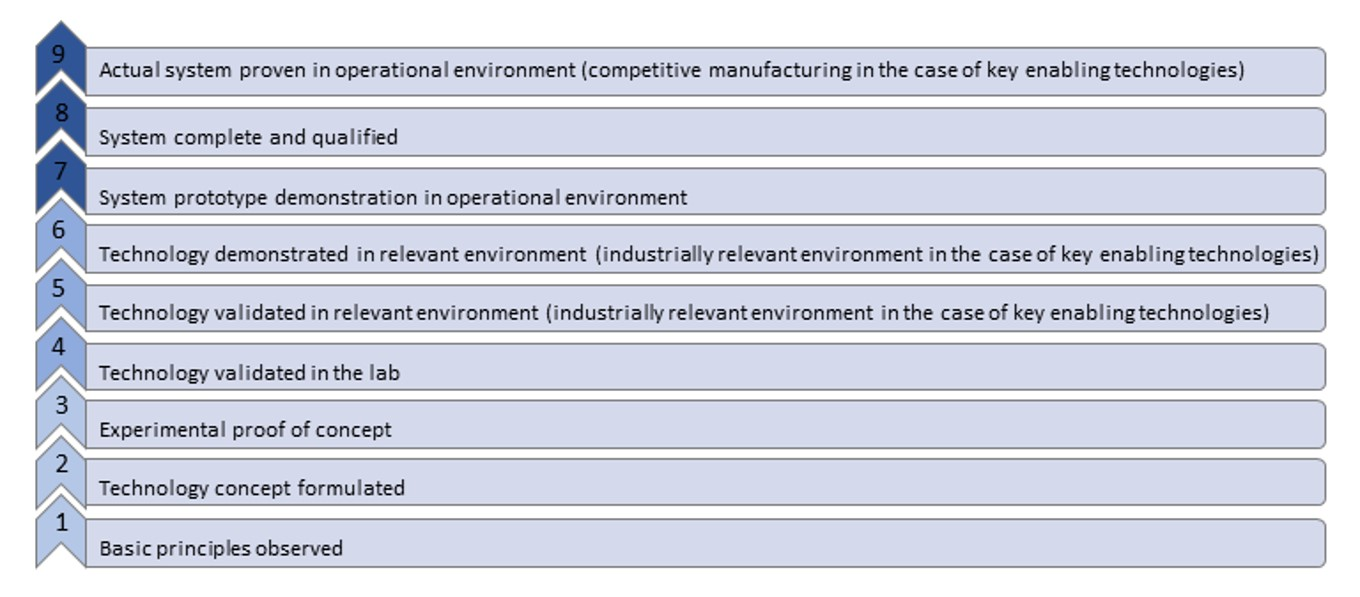
\includegraphics[width=0.9\linewidth]{image/TRL_cropped} \caption{Technology readiness scale}\label{fig:unnamed-chunk-2}
\end{figure}

Furthermore, we evaluate the readiness of a given technology to be acceptable in the society and how well it contributes to the public good using \textbf{societal readiness scale} (McCulloch, 2019):

\begin{figure}
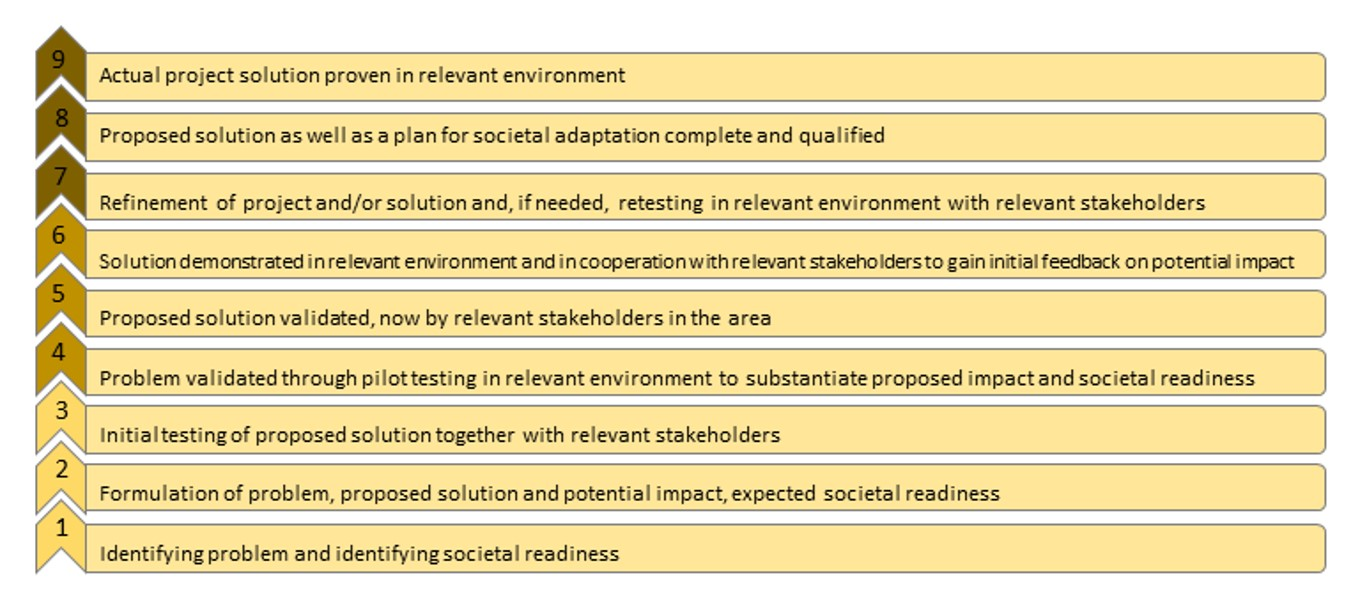
\includegraphics[width=0.9\linewidth]{image/SRL_cropped} \caption{Societal readiness scale}\label{fig:unnamed-chunk-3}
\end{figure}

Finally, we provide a list of \textbf{outstanding questions} and \textbf{links to additional sources} on the topic.

\textbf{References}

\begin{itemize}
\tightlist
\item
  Williamson, R., \& Beasley, J. (2011). \emph{Automotive technology and manufacturing readiness levels: a guide to recognised stages of development within the automotive industry}. URN11/672.
\item
  McCulloch, S. (2019). Social Acceptance And Societal Readiness Levels. {[}online{]} \emph{DecarboN8}. Available at: \url{https://decarbon8.org.uk/social-acceptance-and-societal-readiness-levels/\#:~:text=Societal\%20readiness\%20refers\%20to\%20the,contributes\%20to\%20the\%20public\%20good.} {[}Accessed 21 January 2021{]}.
\end{itemize}

\hypertarget{infrastructure}{%
\chapter{Physical road infrastructure}\label{infrastructure}}

\hypertarget{dedicated_lanes}{%
\section{Dedicated lanes for connected and automated vehicles (CAV)}\label{dedicated_lanes}}

\hypertarget{synonyms}{%
\subsection*{Synonyms}\label{synonyms}}
\addcontentsline{toc}{subsection}{Synonyms}

\emph{AV-dedicated lanes}, \emph{dedicated corridors}

\hypertarget{definition}{%
\subsection*{Definition}\label{definition}}
\addcontentsline{toc}{subsection}{Definition}

Dedicated lane for connected and autonomous vehicles features additional infrastructure or sensors to increase the reliability of Advanced Driver Assistant Systems (ADAS). Only automated driving vehicles are allowed to drive on these lanes. The typical applications include cooperative and adaptive cruise control based on sensors with the infrastructure, lane keeping, fuel use optimization and road pricing possibilities (Broek et al., 2011). The introduction of dedicated lanes for CAV is expected to have direct consequences on the traffic flow on the highways and a nearby road network. In particular, a study conducted in Singapore showed that dedicated lanes on the highways can reduce travel time of CAVs by approximately 25\% (if the saturation on the lane is not reached) at the cost of a delay for conventional cars of approximately 7\%, due to the reduced capacity (Ivanchev et al., 2017). They were also demonstrated to have a positive effect on fuel consumption.
Moreover, the throughput, defined as a number of vehicles passing through the road in a given time interval, increased as a result of introduction of dedicated lanes for AVs (Kumar et al., 2020). This effect, however, was associated with a decrease in throughput of smaller roads due to the preference of AVs for highways because of time savings, which in turn can result in time loss for conventional cars. What is more, the benefits from increased capacity of AV-only lanes can be further amplified through setting a higher speed limits for these lanes (Ye \& Yamamoto, 2018). With respect to the demand for different road types the study found that the introduction of dedicated CAV lanes will increase the demand of conventional cars for major road (but smaller than highways) and minor roads as a substitution for more congested highways due to the dedicated AV lanes.
In contrast, study by Chen et al.~(2016) showed that the implementation of CAV dedicated lanes has a potential of maximizing traffic capacity on these lanes in a mix-traffic context while having effectively no impact on conventional traffic capacity. Further, in order to use efficiently CAV dedicated lanes, which may be underutilized at the early stage, it is proposed to allow conventional cars to enter the AVs-only lanes after toll payment. This solution stems from currently operational across the world High Occupancy Vehicle (HOV) lanes. This joint approach is claimed to improve the throughput of individual road as well as enhance system-wide flow distribution within the network (Liu \& Song, 2019).

\hypertarget{key-stakeholders}{%
\subsection*{Key stakeholders}\label{key-stakeholders}}
\addcontentsline{toc}{subsection}{Key stakeholders}

\begin{itemize}
\tightlist
\item
  \textbf{Affected}: Conventional Cars' Drivers, Car Manufacturers, Insurers
\item
  \textbf{Responsible}: Road Infrastructure Agencies, Local and National Governments
\end{itemize}

\hypertarget{current-state-of-art-in-research}{%
\subsection*{Current state of art in research}\label{current-state-of-art-in-research}}
\addcontentsline{toc}{subsection}{Current state of art in research}

Current research focuses on gathering the evidence of the impact of the introduction of dedicated lanes on traffic flow, driver behavior adoption, safety and efficiency. Furthermore, it analyses the factors which influence them, by testing different design and operation configurations, road types and utilization policies (Rad et al., 2020). Both, field operational testing and driving simulator studies have been conducted to investigate the influence of different designs of dedicated lanes on drivers in conventional cars and those featuring some degree of automation (Guin et al., 2008, Zhong, 2018). In particular, a number of studies compared distinct access types of dedicated lanes (Zhong, 2018, Yang et al., 2019). They showed that dedicated lanes with limited access performed better in terms of travel time and throughput compared to dedicated lanes with continuous access. Moreover, the probability of vehicles platooning was significantly higher on dedicated lanes with limited access. On the other hand, it was showed that collision rates near the entry or exit of these limited access lanes are higher (Rad et al.~2020).

\hypertarget{current-state-of-art-in-practice}{%
\subsection*{Current state of art in practice}\label{current-state-of-art-in-practice}}
\addcontentsline{toc}{subsection}{Current state of art in practice}

Currently state of Michigan together with several private partners including Ford and Alphabet Inc.~are planning to dedicate 65 km of a highway between Detroit and Ann Arbor for the sole movement of autonomous vehicles including buses and shuttles (Krisher \& Eggert, 2020). Similar initiatives are taking place in other countries, for instance, China set out to build nearly 100 km of 8-lane highway linking Beijing and the Xiongan New Area, from which 2 lanes will be allocated for the automated traffic. The completion of the construction phase is predicted by the end of 2020, while its opening is for traffic is expected in June 2021 (Syncedreview.com, 2020). In Europe, there is on-going SHOW (SHared automation Operating models for Worldwide adoption) project which aims to deploy about seventy automated vehicles in 21 European cities. To assess how they can best be integrated vehicles will be used in different settings in mixed traffic and dedicated lanes. However, for safety reasons the driver will be on-board (CORDIS, 2020).

\hypertarget{relevant-initiatives-in-austria}{%
\subsection*{Relevant initiatives in Austria}\label{relevant-initiatives-in-austria}}
\addcontentsline{toc}{subsection}{Relevant initiatives in Austria}

\begin{itemize}
\tightlist
\item
  \href{https://www.tugraz.at/fileadmin/user_upload/Institute/IHF/Projekte/ENABLE-S3_SummaryofResults_May2019.pdf}{tugraz.at}
\item
  \href{https://www.ait.ac.at/themen/verkehrssicherheit-und-unfallforschung/projects/via-autonom/}{ait.ac.at}
\end{itemize}

\hypertarget{impacts-with-respect-to-sustainable-development-goals-sdgs}{%
\subsection*{Impacts with respect to Sustainable Development Goals (SDGs)}\label{impacts-with-respect-to-sustainable-development-goals-sdgs}}
\addcontentsline{toc}{subsection}{Impacts with respect to Sustainable Development Goals (SDGs)}

\begin{longtable}[]{@{}ccccc@{}}
\toprule
\begin{minipage}[b]{0.17\columnwidth}\centering
Impact level\strut
\end{minipage} & \begin{minipage}[b]{0.16\columnwidth}\centering
Indicator\strut
\end{minipage} & \begin{minipage}[b]{0.17\columnwidth}\centering
Impact direction\strut
\end{minipage} & \begin{minipage}[b]{0.17\columnwidth}\centering
Goal description and number\strut
\end{minipage} & \begin{minipage}[b]{0.17\columnwidth}\centering
Source\strut
\end{minipage}\tabularnewline
\midrule
\endhead
\begin{minipage}[t]{0.17\columnwidth}\centering
Individual\strut
\end{minipage} & \begin{minipage}[t]{0.16\columnwidth}\centering
Fuel consumption reduced\strut
\end{minipage} & \begin{minipage}[t]{0.17\columnwidth}\centering
\textbf{+}\strut
\end{minipage} & \begin{minipage}[t]{0.17\columnwidth}\centering
Environmental sustainability (\emph{7,12,13,15})\strut
\end{minipage} & \begin{minipage}[t]{0.17\columnwidth}\centering
Ivanchev et al., 2017\strut
\end{minipage}\tabularnewline
\begin{minipage}[t]{0.17\columnwidth}\centering
Individual\strut
\end{minipage} & \begin{minipage}[t]{0.16\columnwidth}\centering
Travel time reduced\strut
\end{minipage} & \begin{minipage}[t]{0.17\columnwidth}\centering
\textbf{+}\strut
\end{minipage} & \begin{minipage}[t]{0.17\columnwidth}\centering
Sustainable economic development (\emph{8,11})\strut
\end{minipage} & \begin{minipage}[t]{0.17\columnwidth}\centering
Zhong, 2018; Yang et al., 2019\strut
\end{minipage}\tabularnewline
\begin{minipage}[t]{0.17\columnwidth}\centering
Systemic\strut
\end{minipage} & \begin{minipage}[t]{0.16\columnwidth}\centering
Collision rate reduced\strut
\end{minipage} & \begin{minipage}[t]{0.17\columnwidth}\centering
\textbf{+}\strut
\end{minipage} & \begin{minipage}[t]{0.17\columnwidth}\centering
Health \& Wellbeing (\emph{3})\strut
\end{minipage} & \begin{minipage}[t]{0.17\columnwidth}\centering
Zhang et al., 2020\strut
\end{minipage}\tabularnewline
\begin{minipage}[t]{0.17\columnwidth}\centering
Systemic\strut
\end{minipage} & \begin{minipage}[t]{0.16\columnwidth}\centering
Emissions rate reduced\strut
\end{minipage} & \begin{minipage}[t]{0.17\columnwidth}\centering
\textbf{+}\strut
\end{minipage} & \begin{minipage}[t]{0.17\columnwidth}\centering
Environmental sustainability (\emph{7,12,13,15})\strut
\end{minipage} & \begin{minipage}[t]{0.17\columnwidth}\centering
Al Alam at al., 2010\strut
\end{minipage}\tabularnewline
\begin{minipage}[t]{0.17\columnwidth}\centering
Systemic\strut
\end{minipage} & \begin{minipage}[t]{0.16\columnwidth}\centering
Congestion\strut
\end{minipage} & \begin{minipage}[t]{0.17\columnwidth}\centering
\textbf{\textasciitilde{}}\strut
\end{minipage} & \begin{minipage}[t]{0.17\columnwidth}\centering
Sustainable economic development (\emph{8,11})\strut
\end{minipage} & \begin{minipage}[t]{0.17\columnwidth}\centering
Ivanchev et al., 2017; Kumar et al., 2020\strut
\end{minipage}\tabularnewline
\begin{minipage}[t]{0.17\columnwidth}\centering
Systemic\strut
\end{minipage} & \begin{minipage}[t]{0.16\columnwidth}\centering
Novel designs tested\strut
\end{minipage} & \begin{minipage}[t]{0.17\columnwidth}\centering
\textbf{+}\strut
\end{minipage} & \begin{minipage}[t]{0.17\columnwidth}\centering
Innovation \& Infrastructure (\emph{9})\strut
\end{minipage} & \begin{minipage}[t]{0.17\columnwidth}\centering
Guin et al., 2008; Zhong, 2018; Krisher \& Eggert, 2020\strut
\end{minipage}\tabularnewline
\begin{minipage}[t]{0.17\columnwidth}\centering
Systemic\strut
\end{minipage} & \begin{minipage}[t]{0.16\columnwidth}\centering
SHOW EU initiative\strut
\end{minipage} & \begin{minipage}[t]{0.17\columnwidth}\centering
\textbf{+}\strut
\end{minipage} & \begin{minipage}[t]{0.17\columnwidth}\centering
Partnership \& collaborations (\emph{17})\strut
\end{minipage} & \begin{minipage}[t]{0.17\columnwidth}\centering
CORDIS, 2020\strut
\end{minipage}\tabularnewline
\bottomrule
\end{longtable}

\hypertarget{technology-and-societal-readiness-level}{%
\subsection*{Technology and societal readiness level}\label{technology-and-societal-readiness-level}}
\addcontentsline{toc}{subsection}{Technology and societal readiness level}

\begin{longtable}[]{@{}cc@{}}
\toprule
TRL & SRL\tabularnewline
\midrule
\endhead
5-6 & 1-3\tabularnewline
\bottomrule
\end{longtable}

\hypertarget{open-questions}{%
\subsection*{Open questions}\label{open-questions}}
\addcontentsline{toc}{subsection}{Open questions}

\begin{enumerate}
\def\labelenumi{\arabic{enumi}.}
\tightlist
\item
  What are the potential benefits of dedicated AV lanes when coupled with smart platooning strategies?
\item
  How and to what degree will joint concepts by automotive sector, fleet and road
  operators will improve traffic management establishing dynamic traffic regulations even across
  borders?
\item
  What are the roles and responsibilities of the different stakeholders of physical infrastructure for connected and automated vehicles?
\item
  Should the vehicle cope with any road infrastructure, and if not, what demands can be set to adapt the existing infrastructure?
\item
  How to ensure continuity between those different environments?
\item
  Which tools (e.g.~micro- and macroscopic transport modelling, impact assessment) can enable
  cities to assess the impact of automated vehicles on their physical road infrastructure and
  balance the needs of automated vehicles against the needs of existing modes (conventional
  vehicles, public transport, pedestrians and cyclists). (ERTRAC, 2019)
\end{enumerate}

\hypertarget{further-links}{%
\subsection*{Further links}\label{further-links}}
\addcontentsline{toc}{subsection}{Further links}

\begin{itemize}
\tightlist
\item
  \href{https://knowledge-base.connectedautomateddriving.eu/wp-content/uploads/2019/12/SMART_2010-0064-study-report-final_V1-2.pdf}{knowledge base}
\item
  \href{https://show-project.eu/}{show project}
\end{itemize}

\hypertarget{references}{%
\subsection*{References}\label{references}}
\addcontentsline{toc}{subsection}{References}

\begin{itemize}
\tightlist
\item
  Al Alam, A., Gattami, A., \& Johansson, K. H. (2010, September). An experimental study on the fuel reduction potential of heavy duty vehicle platooning. In 13th International IEEE Conference on Intelligent Transportation Systems (pp.~306-311). IEEE.
  Broek, S. M., van Nunen, E., \& Zwijnenberg, H. (2011). Definition of necessary vehicle and infrastructure systems for automated driving. Retrieved January, 3, 2017.
\item
  Chen, Z., He, F., Zhang, L., \& Yin, Y. (2016). Optimal deployment of autonomous vehicle lanes with endogenous market penetration. Transportation Research Part C: Emerging Technologies, 72, 143-156.
\item
  CORDIS \textbar{} European Commission. (20 Apr 2020). Retrieved 13 November 2020, from \url{https://cordis.europa.eu/project/id/875530}
\item
  ERTRAC Working Group. (2019). Connected Automated Driving Roadmap. version, 8, 2019-08.
\item
  Guin, A., Hunter, M., \& Guensler, R. (2008). Analysis of reduction in effective capacities of high-occupancy vehicle lanes related to traffic behavior. Transportation Research Record, 2065(1), 47-53.
\item
  Ivanchev, J., Knoll, A., Zehe, D., Nair, S., \& Eckhoff, D. (2017). Potentials and implications of dedicated highway lanes for autonomous vehicles. arXiv preprint arXiv:1709.07658.
\item
  Krisher, T., \& Eggert, D. (14 Aug 2020). Michigan plans dedicated road lanes for autonomous vehicles. Retrieved 12 November 2020, from \url{https://abcnews.go.com/Technology/wireStory/michigan-plans-dedicated-road-lanes-autonomous-vehicles-72352758}
\item
  Kumar, A., Guhathakurta, S., \& Venkatachalam, S. (2020). When and where should there be dedicated lanes under mixed traffic of automated and human-driven vehicles for system-level benefits?. Research in Transportation Business \& Management, 100527.
\item
  Liu, Z., \& Song, Z. (2019). Strategic planning of dedicated autonomous vehicle lanes and autonomous vehicle/toll lanes in transportation networks. Transportation Research Part C: Emerging Technologies, 106, 381-403.
\item
  Rad, S. R., Farah, H., Taale, H., van Arem, B., \& Hoogendoorn, S. P. (2020). Design and operation of dedicated lanes for connected and automated vehicles on motorways: A conceptual framework and research agenda. Transportation Research Part C: Emerging Technologies, 117, 102664.
\item
  Syncedreview.com (31 Aug 2020). Beijing Builds 100km Highway Lanes for Self-Driving Cars with Unmanned Machineries. Retrieved 12 November 2020, from \url{https://syncedreview.com/2020/08/31/beijing-builds-100km-highway-lanes-for-self-driving-cars-with-unmanned-machineries/}
\item
  Yang, D., Farah, H., Schoenmakers, M. J., \& Alkim, T. (2019). Human drivers behavioural adaptation when driving next to a platoon of automated vehicles on a dedicated lane and implications on traffic flow: a driving simulator and microscopic simulation study in the Netherlands. In 98th Annual Meeting of the Transportation Research Board (pp.~19-00582).
\item
  Ye, L., \& Yamamoto, T. (2018). Impact of dedicated lanes for connected and autonomous vehicle on traffic flow throughput. Physica A: Statistical Mechanics and its Applications, 512, 588-597.
\item
  Zhang, J., Wu, K., Cheng, M., Yang, M., Cheng, Y., \& Li, S. (2020). Safety Evaluation for Connected and Autonomous Vehicles' Exclusive Lanes considering Penetrate Ratios and Impact of Trucks Using Surrogate Safety Measures. Journal of advanced transportation, 2020.
\item
  Zhong, Z. (2018). Assessing the effectiveness of managed lane strategies for the rapid deployment of cooperative adaptive cruise control technology.
\end{itemize}

\hypertarget{ODD}{%
\section{Operational design domains}\label{ODD}}

\hypertarget{rail_crossing_info_system}{%
\section{Rail crossing information system}\label{rail_crossing_info_system}}

\hypertarget{ers}{%
\section{Electric road system}\label{ers}}

\hypertarget{synonyms-1}{%
\subsection*{Synonyms}\label{synonyms-1}}
\addcontentsline{toc}{subsection}{Synonyms}

\emph{ERS}

\hypertarget{definition-1}{%
\subsection*{Definition}\label{definition-1}}
\addcontentsline{toc}{subsection}{Definition}

Electric Road System (ERS) is a technological solution that is aimed at charging and transferring power from the road to the vehicles driving along that road. It can be considered an alternative for sustainable transport where it ssupports the use of hybrid and electric vehicles. There are three main types of ERS (Muelaner, 2020):

\begin{itemize}
\item
  \textbf{Catenary Systems} are overhead lines suspended about 5 meters above the road which are typically used for trams and electric vehicles but sometimes can also be used along highways to power heavy commercial vehicles. Overhead lines are cheapest and the most mature form of ERS because of their resemblance with power systems used for railways or trams. They require vehicle to be equipped with pantograph which connects it with the line accommodating lateral and vertical movements. For this reason, catenary systems are the most suitable for large commercial vehicles and the lack of compatibility with small, private cars is considered a major disadvantage. What is more, the overhead lines provide a major hazard in case of road accidents for all road users. Moreover, they negatively impact the visual aspects within the areas in which they are installed, potentially posing issues for public acceptance (Muelaner, 2020).
\item
  \textbf{Conductive tracks} are metal rails which are embedded on (or into) the road surface and provide power through a contact with a pick-up point underneath the vehicle. For safety reasons tracks are divided into small segments rather than continuous, so that the electrical connection is running only when the vehicle passes over them. In contrast to overhead lines, the conductive tracks can be used for vehicles of different sizes. Their advantage is also clear in terms of lower installation costs. Sweden has been a testing ground for larger scale use of this electric road system (Muelaner, 2020).
\item
  \textbf{Inductive tracks} are conductive coils which are placed below the surface of the road to provide energy by inducing an electric current in the coil placed under the vehicle driving along the track. Their advantage is smaller maintenance requirement as compared to conductive tracks, however, a system failure would require costly work to access underground infrastructure.
\end{itemize}

Overall, the wider use of ERS would reduce the need for construction of costly charging station, eliminate waiting time while the vehicle is charging, significantly increase driving range of hybrid and electric vehicles and facilitate reduction in size of batteries installed in the private cars which directly translates into more efficient performance.

\hypertarget{key-stakeholders-1}{%
\subsection*{Key stakeholders}\label{key-stakeholders-1}}
\addcontentsline{toc}{subsection}{Key stakeholders}

\begin{itemize}
\tightlist
\item
  \textbf{Affected}: Private and commercial drivers, Private transportation companies, General public
\item
  \textbf{Responsible}: Local councils, National governments, Construction comapnies, Power and petroleum companies, Road power technology firms, Automotive manufacturers
\end{itemize}

\hypertarget{current-state-of-art-in-research-1}{%
\subsection*{Current state of art in research}\label{current-state-of-art-in-research-1}}
\addcontentsline{toc}{subsection}{Current state of art in research}

Current, research focuses on testing of the ERS solutions to enable deployment on a larger scale, extend applicability to a new type of vehicles, increase their efficiency and assess their transport decarbonization potential.

Since 2008 the South Korean company \href{https://www.kaist.ac.kr/en/html/kaist/01200103.html}{OLEV} (branch of KAIST University) has been working on inductive power transfer and since 2013 two electric buses have been in operation on public roads, inside university campus (Kelion, 2013). Nonetheless, this system is currently outdated and results as a low-speed system within local public transport. In 2016 an initial testing of the overhead lines has been conducted in Germany on Siemens' 2 km test track in Berlin, at the same time in Sweden a full integration with Scania vehicle has been achieved. More example include Volvo and Alstom's cooparation on testing of conductive tracks on the 400 m test side in Hällered, Sweden (Möller, 2017). Similarly, Swedish Transport Administration in collaboration with Elonroad under \href{https://www.evolutionroad.se/en/}{EVolution Road} project constructed a 1 km of demonstration road in Lund to test the performance of an electric bus.
On the other hand, research on the efficiency of inductive tracks conducted in France and Italy showed that their performance depends on the precision of alignment between the track and the coil in the vehicle (Muelaner, 2020). Finally, a study by Börjesson et al.~(2020) showed that use of electric road solution can decrease operational costs for freight operators due to a switch from diesel to electricity. Consequently, the social benefit of this technological solution outweighs its cost. Moreover, it has been concluded that use of ERS offers significant reduction in carbon emissions.

\hypertarget{current-state-of-art-in-practice-1}{%
\subsection*{Current state of art in practice}\label{current-state-of-art-in-practice-1}}
\addcontentsline{toc}{subsection}{Current state of art in practice}

At the moment, there are multiple companies offering power technologies such as \href{https://elways.se/}{Elways}, \href{https://www.alstom.com/}{Alstom} or \href{https://elonroad.com/}{Elonroad}, to name a few. The proliferation of such companies enabled active testing and implementation of different ERS solutions around the world.

Since 2016 overhead lines have been successfully deployed on public roads in Sweden (E16 highway outside Gävle) and the USA (City of Carson). Currently, in Germany three tests sponsored by Federal Ministry for the Environment, Nature Conservation and Nuclear Safety \href{www.bmu.de}{(BMU)} are taking place. In Hesse and Schleswig-Holstein 5 km of motorway was electrified at the beginning of 2020 (Wettengel, 2019) while in Baden-Württemberg, 4 km of a national highway will have an overhead line system in operation at the beginning of 2021. For the moment, these overhead lines provide power to freight vehicles, however an issue arises among the truck fleets going through Germany from Eastern Europe, because they are lacking modern hybrid trucks equipped with pantographs on the roof.

Further, between 2016-2017 project \href{https://www.fcirce.es/en/smart-mobility-en-en/victoria-2}{VICTORIA} led by Spanish energy company Endesa developed first dynamic inductive load systems for a bus line in Malaga, Spain. Similarly, EU project \href{https://trimis.ec.europa.eu/project/feasibility-analysis-and-development-road-charging-solutions-future-electric-vehicles}{FABRIC} has been conducted in Torino, Italy and Satory in France (Tongur \& Sundelin, 2016).

In terms of cost analysis, an example from the UK shows that inductive tracks provide cost advantage, where the installation of 1 mile (1,6 km) of inductive tracks on a two-lane road costs around 1.4 million euros. If these were to be installed in all UK highways the costs would come up to around 13 billion euros. At the same time, the cost of additional electricity capacity required for hydrogen in \protect\hyperlink{FCEV}{FCEV} sums up to 140 billion euros. Additionally, cost-benefit analysis showed that if most vehicles used ERS, the savings resulting from smaller batteries in electric cars would outweigh the costs of ERS construction.

Interestingly, ERS has not been particularly popular in Austria, potentially due to presence of well-developed railway network which, thus far, dominated freight. In particular, critics describe the construction of electric highways as \emph{a waste of money}, because it only benefits companies that equip their fleets with the necessary vehicles with overhead line system (Traktuell.at. 2020).

\hypertarget{relevant-initiatives-in-austria-1}{%
\subsection*{Relevant initiatives in Austria}\label{relevant-initiatives-in-austria-1}}
\addcontentsline{toc}{subsection}{Relevant initiatives in Austria}

\begin{itemize}
\tightlist
\item
  \href{https://www.scania.com/at/de/home/products-and-services/trucks/sustainability/elektro-mobilitaet/oberleitungs-lkw.html}{scania.com}
\item
  \href{https://www.electrive.net/2019/07/24/auswertung-der-these-zu-lastkraftwagen-an-oberleitungen/}{electrive.net}
\end{itemize}

\hypertarget{impacts-with-respect-to-sustainable-development-goals-sdgs-1}{%
\subsection*{Impacts with respect to Sustainable Development Goals (SDGs)}\label{impacts-with-respect-to-sustainable-development-goals-sdgs-1}}
\addcontentsline{toc}{subsection}{Impacts with respect to Sustainable Development Goals (SDGs)}

\begin{longtable}[]{@{}ccccc@{}}
\toprule
\begin{minipage}[b]{0.17\columnwidth}\centering
Impact level\strut
\end{minipage} & \begin{minipage}[b]{0.16\columnwidth}\centering
Indicator\strut
\end{minipage} & \begin{minipage}[b]{0.17\columnwidth}\centering
Impact direction\strut
\end{minipage} & \begin{minipage}[b]{0.17\columnwidth}\centering
Goal description and number\strut
\end{minipage} & \begin{minipage}[b]{0.17\columnwidth}\centering
Source\strut
\end{minipage}\tabularnewline
\midrule
\endhead
\begin{minipage}[t]{0.17\columnwidth}\centering
Individual\strut
\end{minipage} & \begin{minipage}[t]{0.16\columnwidth}\centering
Potential for lowering purchasing price of electric cars with smaller battery requirement\strut
\end{minipage} & \begin{minipage}[t]{0.17\columnwidth}\centering
\textbf{+}\strut
\end{minipage} & \begin{minipage}[t]{0.17\columnwidth}\centering
Sustainable economic development (\emph{8,11})\strut
\end{minipage} & \begin{minipage}[t]{0.17\columnwidth}\centering
Muelaner, 2020\strut
\end{minipage}\tabularnewline
\begin{minipage}[t]{0.17\columnwidth}\centering
Systemic\strut
\end{minipage} & \begin{minipage}[t]{0.16\columnwidth}\centering
Reduction in emissions and use of fossil fuels\strut
\end{minipage} & \begin{minipage}[t]{0.17\columnwidth}\centering
\textbf{+}\strut
\end{minipage} & \begin{minipage}[t]{0.17\columnwidth}\centering
Environmental sustainability (\emph{7,12,13,15})\strut
\end{minipage} & \begin{minipage}[t]{0.17\columnwidth}\centering
Tongur \& Sundelin, 2016; Moeller, 2017; Boerjesson et al., 2020\strut
\end{minipage}\tabularnewline
\begin{minipage}[t]{0.17\columnwidth}\centering
Systemic\strut
\end{minipage} & \begin{minipage}[t]{0.16\columnwidth}\centering
Cost saving compared to hybrid vehicles; long-term maintenance costs uncertain\strut
\end{minipage} & \begin{minipage}[t]{0.17\columnwidth}\centering
\textbf{\textasciitilde{}}\strut
\end{minipage} & \begin{minipage}[t]{0.17\columnwidth}\centering
Sustainable economic development (\emph{8,11})\strut
\end{minipage} & \begin{minipage}[t]{0.17\columnwidth}\centering
Muelaner, 2020; Boerjesson et al., 2020\strut
\end{minipage}\tabularnewline
\begin{minipage}[t]{0.17\columnwidth}\centering
Systemic\strut
\end{minipage} & \begin{minipage}[t]{0.16\columnwidth}\centering
Novel designs tested\strut
\end{minipage} & \begin{minipage}[t]{0.17\columnwidth}\centering
\textbf{+}\strut
\end{minipage} & \begin{minipage}[t]{0.17\columnwidth}\centering
Innovation \& Infrastructure (\emph{9})\strut
\end{minipage} & \begin{minipage}[t]{0.17\columnwidth}\centering
Kelion, 2013\strut
\end{minipage}\tabularnewline
\begin{minipage}[t]{0.17\columnwidth}\centering
Systemic\strut
\end{minipage} & \begin{minipage}[t]{0.16\columnwidth}\centering
Increased cross-industrial collaboration\strut
\end{minipage} & \begin{minipage}[t]{0.17\columnwidth}\centering
\textbf{+}\strut
\end{minipage} & \begin{minipage}[t]{0.17\columnwidth}\centering
Partnership \& collaborations (\emph{17})\strut
\end{minipage} & \begin{minipage}[t]{0.17\columnwidth}\centering
Kelion, 2013; Wettengel, 2019\strut
\end{minipage}\tabularnewline
\bottomrule
\end{longtable}

\hypertarget{technology-and-societal-readiness-level-1}{%
\subsection*{Technology and societal readiness level}\label{technology-and-societal-readiness-level-1}}
\addcontentsline{toc}{subsection}{Technology and societal readiness level}

\begin{longtable}[]{@{}cc@{}}
\toprule
TRL & SRL\tabularnewline
\midrule
\endhead
5-9 & 4-7\tabularnewline
\bottomrule
\end{longtable}

\hypertarget{open-questions-1}{%
\subsection*{Open questions}\label{open-questions-1}}
\addcontentsline{toc}{subsection}{Open questions}

\begin{enumerate}
\def\labelenumi{\arabic{enumi}.}
\tightlist
\item
  What is the potential of the use of ERS beyond freight vehicles?
\item
  How do stakeholders develop new business models that support ERS deployment?
\item
  Do public authorities have to own the electric roads?
\item
  What are the long-term costs associated with the maintenance of ERS?
\end{enumerate}

\hypertarget{further-links-1}{%
\subsection*{Further links}\label{further-links-1}}
\addcontentsline{toc}{subsection}{Further links}

\begin{itemize}
\tightlist
\item
  \href{https://www.fcirce.es/en/smart-mobility-en-en/victoria-2}{fcirce.es}
\item
  \href{https://www.engineering.com/story/electric-road-systems}{engineering.com}
\item
  \href{https://www.bbc.com/news/technology-23603751}{bbc.com}
\item
  \href{https://www.cleanenergywire.org/news/germany-opens-first-overhead-electricity-test-track-trucks-autobahn}{cleanenergywire.org}
\item
  \href{https://trimis.ec.europa.eu/project/feasibility-analysis-and-development-road-charging-solutions-future-electric-vehicles}{trimis.ec.europa.eu}
\item
  \href{https://www.alstom.com/}{Alstom}
\item
  \href{https://elonroad.com/}{Elonroad}
\item
  \href{https://www.diva-portal.org/smash/get/diva2:1127479/FULLTEXT01.pdf}{KTH report}
\item
  \href{https://www.scania.com/group/en/home/newsroom/news/2016/scania-tests-fast-wireless-charging-in-urban-traffic.html}{Scania}
\item
  \href{https://insideevs.com/news/373644/electrified-roads-sweden-solaris-elonroad/}{insideevs.com}
\item
  \href{https://a3bau.at/so-funktionieren-elektrifizierte-strassen}{a3bau.at}
\item
  \href{https://press.siemens.com/global/de/feature/ehighway-loesungen-fuer-den-elektrifizierten-strassengueterverkehr}{Siemens}
\item
  \href{https://traktuell.at/a/ohne-akzeptanz-kein-ehighway-in-deutschland}{traktuell.at}
\end{itemize}

\hypertarget{references-1}{%
\subsection*{References}\label{references-1}}
\addcontentsline{toc}{subsection}{References}

\begin{itemize}
\tightlist
\item
  Börjesson, M., Johansson, M., \& Kågeson, P. (2020). The economics of electric roads.
\item
  Kelion, L., 2013. South Korean road wirelessly recharges OLEV buses. {[}online{]} BBC News. Available at: \url{https://www.bbc.com/news/technology-23603751} {[}Accessed 19 February 2021{]}.
\item
  Möller, C. (2017). Carbon neutral road transportation: an assessment of the potential of electrified road systems.
\item
  Muelaner, J., 2020. Electric Road Systems. {[}online{]} Engineering.com. Available at: \url{https://www.engineering.com/story/electric-road-systems} {[}Accessed 18 February 2021{]}.
\item
  Tongur, S., \& Sundelin, H. (2016, October). The electric road system transition from a system to a system-of-systems. In 2016 Asian Conference on Energy, Power and Transportation Electrification (ACEPT) (pp.~1-8). IEEE.
\item
  Traktuell.at. 2020. Ohne Akzeptanz kein eHighway in Deutschland. {[}online{]} Available at: \url{https://traktuell.at/a/ohne-akzeptanz-kein-ehighway-in-deutschland} {[}Accessed 19 February 2021{]}.
\item
  Wettengel, J., 2019. Germany opens first overhead electricity test track for trucks on autobahn. {[}online{]} Clean Energy Wire. Available at: \url{https://www.cleanenergywire.org/news/germany-opens-first-overhead-electricity-test-track-trucks-autobahn} {[}Accessed 19 February 2021{]}.
\end{itemize}

\hypertarget{high_occupancy}{%
\section{High occupancy toll lanes}\label{high_occupancy}}

\hypertarget{public_trans_priority}{%
\section{Public transport priority systems}\label{public_trans_priority}}

\hypertarget{synonyms-2}{%
\subsection*{Synonyms}\label{synonyms-2}}
\addcontentsline{toc}{subsection}{Synonyms}

\emph{pre-emption of public transport vehicles, public transport priority (PTP), Transit signal priority (TSP), road-space priority (RSP)}

\hypertarget{definition-2}{%
\subsection*{Definition}\label{definition-2}}
\addcontentsline{toc}{subsection}{Definition}

To encourage people to use public transport and thereby travel more sustainably, it is necessary that public transport operates reliably and efficiently. For example, public transport is the most efficient mode of transport at the intersections, where the difference in the number of people who can pass through a junction in a given time is particularly impressive between cars and public transport. The ratio is between 1 to 10 and 1 to 20 (Schwendinger, 2019). In contrast, a bus at full capacity that is stuck in congestion increases the travel time of many more passengers, compared to single cars in a similar position. Time delays due to traffic signals account for up to 25\% of the total travel time of buses (Seredynski et al., 2015). Furthermore, energy prices and emissions generated become more relevant for public transport operators, to compete with the motorized private transport (Gassel et al., 2012).
The implementation of public transport priority measures can help improving time and energy efficiency of public transport service. The delays caused by traffic signals can be reduced by the introduction of Transit Signal Priority (TSP) such as early green, green extension, phase rotation, phase insertion and actuated transit phase, favouring public transport (Seredynski et al., 2015). TSP systems can increase the attractiveness of public transport, reduce the operation cost and reduce tailpipe emissions and energy use. On the other hand, they increase the travel time of general traffic, therefore the acceptance is limited (Seredynski et al., 2015). Another widely used systems are separated bus lanes or independent tracks for trams. These are especially relevant in 30 km/h zones, so the public transport vehicles can be excluded from the regulation. But since space is a limited good, independent lanes or tracks are not always possible to implement (Schwendinger, 2019).
For Vienna priority of public transport vehicles is of high importance (WIENER STADTWERKE GmbH, 2018). The first measures to shorten the travel time of the bus route 15A at Wienerberg took effect in Autumn 2018. Measures to give priority to public transport are also becoming more important in other cities such as Linz, Graz or Innsbruck. Trams in Graz have priority switching at almost all traffic lights, while there is a further need for bus lines, especially for those from the surrounding area (Schwendinger, 2019).To promote e-mobility, some countries introduced bus lane access to e-vehicles (Figenbaum et al., 2015). Wiener Linien is clearly against this measure, because cars, regardless of their propulsion system, cause delays in the bus lanes and slow down public transport (WIENER STADTWERKE GmbH, 2018).

\hypertarget{key-stakeholders-2}{%
\subsection*{Key stakeholders}\label{key-stakeholders-2}}
\addcontentsline{toc}{subsection}{Key stakeholders}

\begin{itemize}
\tightlist
\item
  \textbf{Affected}: Road Users, Public Transport Users, Public Transport Operators
\item
  \textbf{Responsible}: State Authorities, Transport Infrastructure Operators, Technology Providers
\end{itemize}

\hypertarget{current-state-of-art-in-research-2}{%
\subsection*{Current state of art in research}\label{current-state-of-art-in-research-2}}
\addcontentsline{toc}{subsection}{Current state of art in research}

Current research aims at building on the existing solutions such as TSP and proposes so-called Green Light Optimal Speed Advisory (GLOSA) driver assistance systems. A multi segment GLOSA can take several lights in a sequence on route of a bus into account and allows the driver to adjust the speed, so that the bus can arrive at the intersection when the light is green. By that, the comfort of passengers can be increased and the fuel consumption as well as the tailpipe emissions be decreased, without negatively affecting the general traffic (Seredynski et al., 2014). However, Stahlmann et al.~(2018) argue that so far, most GLOSA simulation studies are too optimistic in terms of communication performance and recommend further improvement of GLOSA systems.
Moreover, the Green Light Optimal Dwell Time Advisory (GLODTA) systems look into exploiting additional dwell time at the near-side bus stop (Seredynski et al., 2014). According to Seredynski \& Viti (2017) they can support on-route battery charging of electrical buses and also replace existing holding strategies used to regulate punctuality of bus services.
Due the limited acceptance of TSP systems, more research regarding the efficient use of green time provided to public transport is needed. Therefore, the focus is on the improvement of the bus detection methods. The latest TSP are working with GPS-based Virtual Detectors (VD), which eliminate the need of on-street detection infrastructure, but their disadvantages is low accuracy (Seredynski et al., 2015).
Haitao et al.~(2019) developed an integrated and systematic framework for the optimization of bimodal urban networks using 3D-MFDs, considering the complexities of bimodality to manage traffic more efficiently and provide public transport priority. Results of the evaluation show that the proposed strategy always performs better than existing perimeter control schemes in terms of passenger mobility.

\hypertarget{current-state-of-art-in-practice-2}{%
\subsection*{Current state of art in practice}\label{current-state-of-art-in-practice-2}}
\addcontentsline{toc}{subsection}{Current state of art in practice}

A common measure in use is the positioning of stops before intersections, which combines the standing time at the traffic lights with the passenger change and thus leads to travel time reductions (Schwendinger, 2019).
All around the world Bus Rapid Transit (BRT) systems have gained popularity. Cervero (2013) defines them as ``bus-based system that mimics the high-capacity, high-performance characteristics of urban rail systems at a much lower price'' that runs either on exclusive transit-ways, dedicated bus lanes or some grade of separation.
Regarding TPS, the cloud-based systems using GPS locations are standard technology (see Figure 1). However, there are still many outdated systems in use that are based on short-range radio. These systems require that all traffic lights are equipped with receivers. All buses in a fleet need special transmitters and an onboard system for positioning, which makes it an overall expensive system. At the same time, this technology is rather unreliable and maintenance intensive (SWARCO, 2021).

\begin{figure}
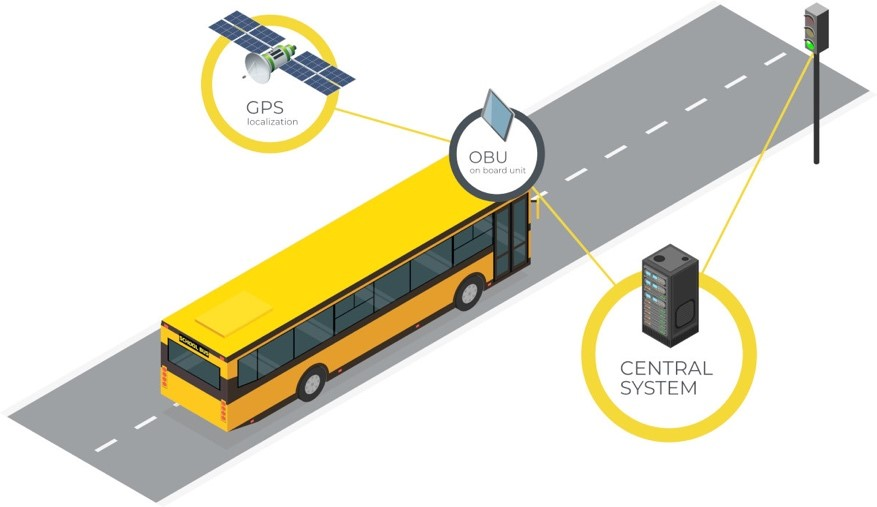
\includegraphics[width=0.7\linewidth]{image/pt_priority_system} \caption{Smart priority for public transport (SWARCO, 2021)}\label{fig:unnamed-chunk-4}
\end{figure}

\hypertarget{relevant-initiatives-in-austria-2}{%
\subsection*{Relevant initiatives in Austria}\label{relevant-initiatives-in-austria-2}}
\addcontentsline{toc}{subsection}{Relevant initiatives in Austria}

\begin{itemize}
\tightlist
\item
  \href{https://digitales.wien.gv.at/site/open-data/}{digitales.wien.gv.at}
\item
  \href{https://www.wienerlinien.at/eportal3/ep/channelView.do/pageTypeId/66528/channelId/-4400661}{wienerlinien.at}
\item
  \href{https://www.kapsch.net/ktc/Portfolio/IMS/Congestion/Managed-lanes}{kapsch.net-1}
\item
  \href{https://www.kapsch.net/ktc/Portfolio/IMS/Smart-Urban-Mobility/Urban-Mobility-Management}{kapsch.net-2}
\item
  \href{https://www.swarco.com/de/loesungen/oeffentlicher-nahverkehr/vorrang-fuer-den-oeffentlichen-nahverkehr}{swarco.com}
\item
  \href{https://www.mobility.siemens.com/global/de/portfolio/strasse/verkehrsmanagement/auf-der-strasse/smart-detection.html}{mobility.siemens.com}
\end{itemize}

\hypertarget{impacts-with-respect-to-sustainable-development-goals-sdgs-2}{%
\subsection*{Impacts with respect to Sustainable Development Goals (SDGs)}\label{impacts-with-respect-to-sustainable-development-goals-sdgs-2}}
\addcontentsline{toc}{subsection}{Impacts with respect to Sustainable Development Goals (SDGs)}

\begin{longtable}[]{@{}ccccc@{}}
\toprule
\begin{minipage}[b]{0.17\columnwidth}\centering
Impact level\strut
\end{minipage} & \begin{minipage}[b]{0.16\columnwidth}\centering
Indicator\strut
\end{minipage} & \begin{minipage}[b]{0.17\columnwidth}\centering
Impact direction\strut
\end{minipage} & \begin{minipage}[b]{0.17\columnwidth}\centering
Goal description and number\strut
\end{minipage} & \begin{minipage}[b]{0.17\columnwidth}\centering
Source\strut
\end{minipage}\tabularnewline
\midrule
\endhead
\begin{minipage}[t]{0.17\columnwidth}\centering
Individual\strut
\end{minipage} & \begin{minipage}[t]{0.16\columnwidth}\centering
Higher equality for people who do not drive\strut
\end{minipage} & \begin{minipage}[t]{0.17\columnwidth}\centering
\textbf{+}\strut
\end{minipage} & \begin{minipage}[t]{0.17\columnwidth}\centering
Equality (\emph{5,10})\strut
\end{minipage} & \begin{minipage}[t]{0.17\columnwidth}\centering
Litman, 2017; Cervero, 2013\strut
\end{minipage}\tabularnewline
\begin{minipage}[t]{0.17\columnwidth}\centering
Individual\strut
\end{minipage} & \begin{minipage}[t]{0.16\columnwidth}\centering
Less travel time for public transport users, more travel time for car users\strut
\end{minipage} & \begin{minipage}[t]{0.17\columnwidth}\centering
\textbf{\textasciitilde{}}\strut
\end{minipage} & \begin{minipage}[t]{0.17\columnwidth}\centering
Sustainable economic development (\emph{8,11})\strut
\end{minipage} & \begin{minipage}[t]{0.17\columnwidth}\centering
Seredynski et al., 2015\strut
\end{minipage}\tabularnewline
\begin{minipage}[t]{0.17\columnwidth}\centering
Systemic\strut
\end{minipage} & \begin{minipage}[t]{0.16\columnwidth}\centering
Public transport becomes more competitive compared to other transport modes\strut
\end{minipage} & \begin{minipage}[t]{0.17\columnwidth}\centering
\textbf{+}\strut
\end{minipage} & \begin{minipage}[t]{0.17\columnwidth}\centering
Equality (\emph{5,10})\strut
\end{minipage} & \begin{minipage}[t]{0.17\columnwidth}\centering
Schwendinger, 2019\strut
\end{minipage}\tabularnewline
\begin{minipage}[t]{0.17\columnwidth}\centering
Systemic\strut
\end{minipage} & \begin{minipage}[t]{0.16\columnwidth}\centering
Less fuel consumption\strut
\end{minipage} & \begin{minipage}[t]{0.17\columnwidth}\centering
\textbf{+}\strut
\end{minipage} & \begin{minipage}[t]{0.17\columnwidth}\centering
Environmental sustainability (\emph{7,12,13,15})\strut
\end{minipage} & \begin{minipage}[t]{0.17\columnwidth}\centering
Gassel et al., 2012; Seredynski et al., 2015\strut
\end{minipage}\tabularnewline
\begin{minipage}[t]{0.17\columnwidth}\centering
Systemic\strut
\end{minipage} & \begin{minipage}[t]{0.16\columnwidth}\centering
Transit is often the most cost-effective mode\strut
\end{minipage} & \begin{minipage}[t]{0.17\columnwidth}\centering
\textbf{+}\strut
\end{minipage} & \begin{minipage}[t]{0.17\columnwidth}\centering
Sustainable economic development (\emph{8,11})\strut
\end{minipage} & \begin{minipage}[t]{0.17\columnwidth}\centering
Litman, 2015\strut
\end{minipage}\tabularnewline
\begin{minipage}[t]{0.17\columnwidth}\centering
Systemic\strut
\end{minipage} & \begin{minipage}[t]{0.16\columnwidth}\centering
More infrastructre for public transport\strut
\end{minipage} & \begin{minipage}[t]{0.17\columnwidth}\centering
\textbf{+}\strut
\end{minipage} & \begin{minipage}[t]{0.17\columnwidth}\centering
Innovation \& Infrastructure (\emph{9})\strut
\end{minipage} & \begin{minipage}[t]{0.17\columnwidth}\centering
Cuthill et al., 2019\strut
\end{minipage}\tabularnewline
\bottomrule
\end{longtable}

\hypertarget{technology-and-societal-readiness-level-2}{%
\subsection*{Technology and societal readiness level}\label{technology-and-societal-readiness-level-2}}
\addcontentsline{toc}{subsection}{Technology and societal readiness level}

\begin{longtable}[]{@{}cc@{}}
\toprule
TRL & SRL\tabularnewline
\midrule
\endhead
4-8 & 5-8\tabularnewline
\bottomrule
\end{longtable}

\hypertarget{open-questions-2}{%
\subsection*{Open questions}\label{open-questions-2}}
\addcontentsline{toc}{subsection}{Open questions}

\begin{enumerate}
\def\labelenumi{\arabic{enumi}.}
\tightlist
\item
  Who is responsible for the implementation of PTP systems?
\item
  How will Vehicle-to-Vehicle (V2V), Vehicle-to-Infrastructure (V2I) and in future Vehicle-to-Pedestrian (V2P) change PTP systems?
\item
  How could also emergency vehicles be prioritised?
\item
  How to deal with mixed fleets - half new, half old?
\item
  What are the benefits compared to the costs?
\item
  Which standards should be used?
\end{enumerate}

\hypertarget{references-2}{%
\subsection*{References}\label{references-2}}
\addcontentsline{toc}{subsection}{References}

\begin{itemize}
\tightlist
\item
  Cervero, R. (2013). Bus rapid transit (BRT): An efficient and competitive mode of public transport (No.~2013-01). Working Paper.
\item
  Cuthill, N., Cao, M., Liu, Y., Gao, X., \& Zhang, Y. (2019). The association between urban public transport infrastructure and social equity and spatial accessibility within the urban environment: An investigation of Tramlink in London. Sustainability, 11(5), 1229.
\item
  Figenbaum, E., Fearnley, N., Pfaffenbichler, P., Hjorthol, R., Kolbenstvedt, M., Jellinek, R., \ldots{} \& Iversen, L. M. (2015). Increasing the competitiveness of e-vehicles in Europe. European transport research review, 7(3), 1-14.
\item
  Gassel, C., Matschek, T., \& Krimmling, J. (2012). Cooperative traffic signals for energy efficient driving in tramway systems. Aspekte der Verkehrstelematik--ausgewählte Veröffentlichungen 2012, 1.
\item
  Haitao, H., Yang, K., Liang, H., Menendez, M., \& Guler, S. I. (2019). Providing public transport priority in the perimeter of urban networks: A bimodal strategy. Transportation Research Part C: Emerging Technologies, 107, 171-192.
\item
  Litman, T. (2015). Evaluating public transit benefits and costs. Victoria, BC, Canada: Victoria Transport Policy Institute.
\item
  Litman, T. (2017). Evaluating Transportation Diversity. Victoria Transport Policy Institute.
\item
  Schwendinger, M. (2019). Vorrang für Busse und Straßenbahnen in Städten. \url{https://vcoe.at/files/vcoe/uploads/Projekte/Factsheets} 2019 Neu/VCÖ-Factsheet ÖV-Bevorrangen.pdf
\item
  Seredynski, M., Khadraoui, D., \& Viti, F. (2015, October). Signal phase and timing (SPaT) for cooperative public transport priority measures. In Proc. 22nd ITS World Congress.
\item
  Seredynski, M., Ruiz, P., Szczypiorski, K., \& Khadraoui, D. (2014, May). Improving bus ride comfort using GLOSA-based dynamic speed optimisation. In 2014 IEEE International Parallel \& Distributed Processing Symposium Workshops (pp.~457-463). IEEE.
\item
  Seredynski, M., \& Viti, F. (2017, October). Novel C-ITS support for electric buses with opportunity charging. In 2017 IEEE 20th International Conference on Intelligent Transportation Systems (ITSC) (pp.~1-6). IEEE.
\item
  Stahlmann, R., Möller, M., Brauer, A., German, R., \& Eckhoff, D. (2018). Exploring GLOSA systems in the field: Technical evaluation and results. Computer Communications, 120, 112-124.
\item
  SWARCO. (2021). Vorrang für den ÖPNV: Öffentliche Verkehrsmittel attraktiver machen. Retrieved 26th January 2021, from \url{https://www.swarco.com/de/loesungen/oeffentlicher-nahverkehr/vorrang-fuer-den-oeffentlichen-nahverkehr}
\item
  WIENER STADTWERKE GmbH. (2018). Wiener Linien: Autos auf Busspuren halten Öffis auf. \url{https://www.wienerstadtwerke.at/eportal3/ep/contentView.do?pageTypeId=71954\&channelId=-51313\&programId=72863\&contentId=4202309\&contentTypeId=1001}
\end{itemize}

\hypertarget{transformation_public_space}{%
\section{Transformation of public space and digital solutions}\label{transformation_public_space}}

\hypertarget{definition-3}{%
\subsection*{Definition}\label{definition-3}}
\addcontentsline{toc}{subsection}{Definition}

The digitalisation of public (and urban) spaces has been developing, giving rise to concepts such as smart city, wise city, U-city, intelligent city etc. However, its real acceleration started in 2010s as a result of industrial initiatives focused on the collection, management, processing and near real-time analysis of big data through the wide-spread of sensors connecting urban spaces, known as Internet of Things (IoT) devices. In the recent years, especially since the outbreak of COVID-19 pandemic, the urban digitalisation reached a new level. For example, in China digital systems for mass surveillance based on facial recognition are being deployed and in other parts of the world legal basis (such as General Data Protection Regulation (GDPR)) have been developed to allow for recording of biometric data in public spaces (Languillon-Aussel, 2021). Beyond surveillance, digitalisation of public spaces is used in many different areas such as payments and pricing, participatory tools or law enforcement, where, for example, in 2020 Singapore initiated the satellite-based urban toll system which allows for tracking any vehicle at any time of the day to implement dynamic pricing for road use and zone access (Languillon-Aussel, 2021).

Current approaches to the digitalisation of public spaces include mobiles apps, high resolution cameras, interactive stands and kiosks providing services and information, but also IoT devices such as sensors and beacons that automatically collect the data. These devices bring potential to improve the quality and coverage of service in public spaces, lower provision and delivery costs, increase safety and security. Nonetheless, they are not without challenges. Potential issues arise due to privacy and security concerns especially when private sector plays a key role (Warbis, 2018), potential technical difficulties such as unreliable Internet connection or unstable electricity supply (Haldrup, 2018) as well as low trust among society members and so called \emph{digital exclusion} of certain social groups (Durand \& Zijlstra, 2020).

\hypertarget{key-stakeholders-3}{%
\subsection*{Key stakeholders}\label{key-stakeholders-3}}
\addcontentsline{toc}{subsection}{Key stakeholders}

\begin{itemize}
\tightlist
\item
  \textbf{Affected}: Citizens
\item
  \textbf{Responsible}: Local and national governments, Private technology companies, Citizens
\end{itemize}

\hypertarget{current-state-of-art-in-research-3}{%
\subsection*{Current state of art in research}\label{current-state-of-art-in-research-3}}
\addcontentsline{toc}{subsection}{Current state of art in research}

The research shows that as a result of higher digitalisation of public spaces and, in particular, increased digitalisation of transport, some groups may become \emph{digitally excluded}. The factors that are linked to vulnerability in terms of access to digitally-based services and transport are:

\begin{itemize}
\tightlist
\item
  \textbf{Age}: The elderly and underaged are particularly disadvantaged due to their lower engagement with technology. In the case of elderly population, the reduction in cognitive abilities and a decline in psychological mechanisms mean that in general, coping with new technologies can be difficult (Harvey et al., 2019; Pangbourne et al., 2010; Durand \& Zijlstra, 2020). On the other hand, children frequently do not have access to digitals forms of payment or cannot use all available modes of transport alone (Durand \& Zijlstra, 2020).
\item
  \textbf{Income and educational level}: People with lower income and education levels are more vulnerable to digital exclusion where, for example, a Dutch report shows that the transition from the offline to the online purchase of a yearly public transport subscription causes issues for people with lower income levels (Durand \& Zijlstra, 2020).
\item
  \textbf{Ethnicity}: The individuals from minorities tend to be more disadvantaged, however, this is frequently linked to other contributing factors such as cultural preferences or economic deprivation (Durand \& Zijlstra, 2020).
\end{itemize}

\hypertarget{current-state-of-art-in-practice-3}{%
\subsection*{Current state of art in practice}\label{current-state-of-art-in-practice-3}}
\addcontentsline{toc}{subsection}{Current state of art in practice}

At the beginning the digitalization of cities and public spaces strongly relied on the hidden, underground network of cables, sensors, connectors and masts which did not play significant role in the everyday life of an average citizen. Nowadays, the digitalization of public spaces incorporates the concept of smart city into the day-to-day life to a much larger extent. There are many ways in which digitalization materializes in public spaces.

One of them is improved \textbf{connectivity} in the form of Wi-Fi hotspots and zones. For example, in New York \href{https://www.link.nyc/}{LinkNYC} created connectivity corridors across five districts where more than 1700 links has allowed approximately 5 million users to connect for free to the country's fastest, most robust public fibre network. Through this service, \emph{LinkNYC} has supported people in accessing charities, using council services, and even applying for jobs (Warbis, 2018). Moreover, \href{https://calvium.com/}{Calvium} uses the improved connectivity to build a sense-of-place through digital-physical journeys of history and heritage, such as in \href{https://calvium.com/projects/battersea-power-station-redevelopment/}{Battersea Power Station} in London (Warbis, 2018).

Then, digitalisation brings the \textbf{transformation of public services} where non-personal data collected from public spaces is used to better understand the users of public spaces and their needs to improve the cities' spaces, infrastructure and provision of public services. For instance, looking at the type of devices connected to WiFi spots or engaging in digital place-making scheme might indicate socio-economic profiles and support councils in delivering the right services to the right people.

Two of such examples are (\emph{1}) \href{https://lbbd.emu-analytics.net/main/(view/950db2c7-1a3b-448d-9b21-444a0ec7b5e0//rightBar:appinfo)?basemapDetail=1\&zoom=5.0\&lng=-0.36613\&lat=54.04187}{Borough Data Explorer} that gathers data for the indicators that either contribute to borough's so-called \emph{Borough Manifesto targets} or feature within borough's \emph{social progress index} (Lbbd.emu-analytics.net, 2021). (\emph{2}) The Australian city of Joondalup partnered with \href{https://www.lakesidejoondalup.com.au/store-directory/telstra-shop/}{Telstra} to test IoT technologies to better monitor environmental factors like temperature, humidity, pollution, light and noise levels in real time (Barns, 2017).

Next, a \textbf{public-private partnership} is crucial for the strong and reliable digital public domain, where technology companies need to understand policy and strategy of local government to identify areas that may be supported through digital deployment. On the other hand, it is important for local government to understand the features of the technology for deployment. This tight cooperation enables the public sector to direct the digitisation of places in ways that work for public good, retaining the publicness of space and place, regardless of who owns, oversees or manages technologies being deployed (Warbis, 2018). The examples of such initatives are \href{https://wegfinder.at/presse/2021/mit-wegfinder-ist-mobility-as-a-service-in-oesterreich-angekommen(1)/}{ÖBB360 wegfinder}, \href{https://austriatech.at/en/insight-into-the-work-of-the-urban-mobility-laboratories/}{Living Labs} and \href{https://www.aspern-seestadt.at/en}{Seestadt Wien}.

Within transport network the digitalisation brings benefits of improved customisation, efficiency and comfort. The examples of such efforts are real-time information on parking spaces availability such as \href{https://www.eparkomat.com/}{eParkomat} in Czech Republic, digital ticketing and scheduling, for instance, \href{https://www.dv-ticketing.com/}{DV Ticketing} or \href{https://www.thetrainline.com/}{Trainline} in the UK, electronic system for car and bike sharing fleets such as \href{https://www.share-now.com/at/en/}{Share-now} or \href{https://www.nextbike.at/de/niederoesterreich/}{Nextbike} etc. For more information on bike and car sharing see sections on \protect\hyperlink{bike_sharing}{bicycle and e-bicycle hire} and \protect\hyperlink{car_sharing}{car shring} in this work.

Finally, public spaces are claimed to be political in nature. In Europe they support and condition the expression of the life in the city and play a role in participatory planning (Languillon-Aussel, 2021; Parkinson, 2012). For example, in 2013 Austrian railways ÖBB aimed at building a \href{https://www.partizipation.at/gueterzentrum_sued.html}{new freight centre} in Vienna that would move freight traffic away from the roads and onto the railways. The new freight centre was meant to replace the one at north-west station (Nordwestbahnhof). From the beginning, the project was intended to actively involve the general public, and the stakeholders were also strongly integrated into the planning. Therefore, before the start of the project, the ÖBB held an information event, which was accompanied by great protests (from the public) against the project. ÖBB tried, probably for this very reason, to involve the stakeholders so intensively in the entire planning process and as a result successfully completed the project.

Therefore, the digitalisation of urban spaces can influence the innovation in participatory tools where it allows the citizens to express opinion and provide feedback to actively contribute to infrastructure planning process and decision-making. This trend gave rise to so-called digital participatory planning (DPP) (Bouzguenda et al., 2020). Some examples of such initiatives include \href{https://mapyour.city/}{Map your city} app, ideas generation platform \href{https://www.involve.org.uk/resources/case-studies/decide-madrid}{Decide Madrid}, \href{https://oscity.nl/}{Open Source City} in the Netherlands, UK feedback platforms \href{https://www.involve.org.uk/resources/knowledge-base/what/public-participation}{Involve} and \href{http://www.changify.org/}{Changify} or arguments visualisation platform called \href{https://www.nesta.org.uk/feature/six-pioneers-digital-democracy/vtaiwan/}{vTaiwan}.

\hypertarget{relevant-initiatives-in-austria-3}{%
\subsection*{Relevant initiatives in Austria}\label{relevant-initiatives-in-austria-3}}
\addcontentsline{toc}{subsection}{Relevant initiatives in Austria}

\begin{itemize}
\tightlist
\item
  \href{https://wegfinder.at/presse/2021/mit-wegfinder-ist-mobility-as-a-service-in-oesterreich-angekommen(1)/}{ÖBB360 wegfinder}
\item
  \href{https://austriatech.at/en/insight-into-the-work-of-the-urban-mobility-laboratories/}{Living Labs}
\item
  \href{https://www.aspern-seestadt.at/en}{Seestadt Wien}
\item
  \href{https://ec.europa.eu/regional_policy/en/projects/Austria/support-for-digital-transformation-in-lower-austria}{House of digitalisation}
\end{itemize}

\hypertarget{impacts-with-respect-to-sustainable-development-goals-sdgs-3}{%
\subsection*{Impacts with respect to Sustainable Development Goals (SDGs)}\label{impacts-with-respect-to-sustainable-development-goals-sdgs-3}}
\addcontentsline{toc}{subsection}{Impacts with respect to Sustainable Development Goals (SDGs)}

\begin{longtable}[]{@{}ccccc@{}}
\toprule
\begin{minipage}[b]{0.17\columnwidth}\centering
Impact level\strut
\end{minipage} & \begin{minipage}[b]{0.16\columnwidth}\centering
Indicator\strut
\end{minipage} & \begin{minipage}[b]{0.17\columnwidth}\centering
Impact direction\strut
\end{minipage} & \begin{minipage}[b]{0.17\columnwidth}\centering
Goal description and number\strut
\end{minipage} & \begin{minipage}[b]{0.17\columnwidth}\centering
Source\strut
\end{minipage}\tabularnewline
\midrule
\endhead
\begin{minipage}[t]{0.17\columnwidth}\centering
Individual\strut
\end{minipage} & \begin{minipage}[t]{0.16\columnwidth}\centering
Diminished access to digitally based transport services for certain groups\strut
\end{minipage} & \begin{minipage}[t]{0.17\columnwidth}\centering
\textbf{-}\strut
\end{minipage} & \begin{minipage}[t]{0.17\columnwidth}\centering
Equality (\emph{5,10})\strut
\end{minipage} & \begin{minipage}[t]{0.17\columnwidth}\centering
Durand \& Zijlstra, 2020\strut
\end{minipage}\tabularnewline
\begin{minipage}[t]{0.17\columnwidth}\centering
Systemic\strut
\end{minipage} & \begin{minipage}[t]{0.16\columnwidth}\centering
Reduced risk for transport-related social exclusion\strut
\end{minipage} & \begin{minipage}[t]{0.17\columnwidth}\centering
\textbf{+}\strut
\end{minipage} & \begin{minipage}[t]{0.17\columnwidth}\centering
Equality (\emph{5,10})\strut
\end{minipage} & \begin{minipage}[t]{0.17\columnwidth}\centering
Harvey et al., 2019; Pangbourne et al., 2010\strut
\end{minipage}\tabularnewline
\begin{minipage}[t]{0.17\columnwidth}\centering
Systemic\strut
\end{minipage} & \begin{minipage}[t]{0.16\columnwidth}\centering
More informed planning and decision-making based on real-time data from IoT\strut
\end{minipage} & \begin{minipage}[t]{0.17\columnwidth}\centering
\textbf{+}\strut
\end{minipage} & \begin{minipage}[t]{0.17\columnwidth}\centering
Innovation \& Infrastructure (\emph{9})\strut
\end{minipage} & \begin{minipage}[t]{0.17\columnwidth}\centering
Barns, 2017, Bouzguenda et al., 2020\strut
\end{minipage}\tabularnewline
\begin{minipage}[t]{0.17\columnwidth}\centering
Systemic\strut
\end{minipage} & \begin{minipage}[t]{0.16\columnwidth}\centering
Increased collaboration between public and private sector\strut
\end{minipage} & \begin{minipage}[t]{0.17\columnwidth}\centering
\textbf{+}\strut
\end{minipage} & \begin{minipage}[t]{0.17\columnwidth}\centering
Partnership \& collaborations (\emph{17})\strut
\end{minipage} & \begin{minipage}[t]{0.17\columnwidth}\centering
Warbis, 2018;\strut
\end{minipage}\tabularnewline
\bottomrule
\end{longtable}

\hypertarget{technology-and-societal-readiness-level-3}{%
\subsection*{Technology and societal readiness level}\label{technology-and-societal-readiness-level-3}}
\addcontentsline{toc}{subsection}{Technology and societal readiness level}

\begin{longtable}[]{@{}cc@{}}
\toprule
TRL & SRL\tabularnewline
\midrule
\endhead
5-9 & 5-8\tabularnewline
\bottomrule
\end{longtable}

\hypertarget{open-questions-3}{%
\subsection*{Open questions}\label{open-questions-3}}
\addcontentsline{toc}{subsection}{Open questions}

\begin{enumerate}
\def\labelenumi{\arabic{enumi}.}
\tightlist
\item
  To what extent does the increasingly important deployment of digital devices in public spaces impact their political dimensions?
\item
  Are digital technologies transforming citizen practices in public spaces and/or do they allow the emergence of new practices?
\item
  By allowing new forms of expression, as well as political and democratic participation online, the virtual space tends to become a new forum. Is digital technology capturing the political functions of public spaces, which have therefore become unnecessary?
\item
  What impacts do the short life cycles of technologies and the changes of technological generations have on the development of public spaces?
\item
  Is digital transforming the designs, shapes, dimensions, and spatiality of public spaces?
\item
  In what ways is the emergence of new tools and skills changing the way public spaces are planned and developed?
\item
  What role do digital technologies play in the representation, imagination, and perception of public spaces?
\item
  For which type(s) of recipient(s) (such as citizen, consumer, user, and inhabitant) are digital technologies deployed in the public space?
\item
  What impacts do they have on the populations frequenting public spaces?
\item
  Do digital technologies promote social exchanges, or on the contrary, do they physically replicate the segregation of digital bubbles?
\item
  What roles has digital played in adapting public spaces to the health crisis of COVID-19?
  (Languillon-Aussel, 2021)
\end{enumerate}

\hypertarget{further-links-2}{%
\subsection*{Further links}\label{further-links-2}}
\addcontentsline{toc}{subsection}{Further links}

\begin{itemize}
\tightlist
\item
  \href{https://agile-city.com/agile-city-research/digital-tools-for-participatory-led-design/}{Agile city}
\item
  \href{https://theconversation.com/surprise-digital-space-isnt-replacing-public-space-and-might-even-help-make-it-better-87173}{An article on city of bits}
\item
  \href{https://archer-soft.com/blog/how-build-real-time-parking-availability-system}{Parking management systems}
\item
  \href{https://jsis.washington.edu/news/internet-of-things-and-privacy-in-public/}{Internet of Things and Privacy in Public}
\end{itemize}

\hypertarget{references-3}{%
\subsection*{References}\label{references-3}}
\addcontentsline{toc}{subsection}{References}

\begin{itemize}
\tightlist
\item
  Barns, S. (2017) Surprise! Digital space isn't replacing public space, and might even help make it better. Available at: \url{https://theconversation.com/surprise-digital-space-isnt-replacing-public-space-and-might-even-help-make-it-better-87173} {[}Accessed 12 April 2021{]}.
\item
  Bouzguenda, I., Alalouch, C., \& Fava, N. (2020). Examining digital participatory planning: maturity assessment in a small Dutch city. Journal of Cleaner Production, 264, 121706.
\item
  Durand, A. \& Zijlstra, T. (2020). The impact of digitalisation on the access to transport services: a literature review. 10.13140/RG.2.2.22686.97600.
\item
  Haldrup, S.,V. (2018). Digitising public service delivery: opportunities and limitations. Available at: \url{https://www.opml.co.uk/blog/digitising-public-service-delivery-opportunities-and-limitations} {[}Accessed 12 April 2021{]}.
\item
  Harvey, J., Guo, W., \& Edwards, S. (2019). Increasing mobility for older travellers through engagement with technology. Transportation Research Part F: Trafc Psychology and Behaviour, 60, 172-184. \url{doi:10.1016/j.trf.2018.10.019}
\item
  Languillon-Aussel, R. (2021). Digitalisation of public spaces: the great urban change? Available at: \url{https://journals.openedition.org/articulo/4518} . {[}Accessed: 9 April 2021{]}
\item
  Lbbd.emu-analytics.net. (2021). Borough Data Explorer. {[}online{]} Available at: \url{https://lbbd.emu-analytics.net/main/(view/950db2c7-1a3b-448d-9b21-444a0ec7b5e0//rightBar:appinfo)?basemapDetail=1\&zoom=4.7\&lng=3.34490\&lat=54.11363} {[}Accessed 12 April 2021{]}.
\item
  Pangbourne, K. (2018). Mobility and Ageing: A Review of Interactions Between Transport and Technology from the Perspective of Older People In A. Curl \& C. Musselwhite (Eds.), Geographies of Transport and Ageing (pp.~51-71). Cham: Springer International Publishing.
\item
  Parkinson J., 2012, Democracy and Public Space: The Physical Sites of Democratic Performance, Oxford: Oxford University Press, 262 p.
\item
  Warbis, M. (2018). Making the Spaces of Cities Smarter: Why cities (and their citizens) should embrace the digital public realm. \textless Available at: \url{https://medium.com/@warbismichelle/making-the-spaces-of-cities-smarter-why-cities-should-embrace-the-digital-public-realm-c12afc810aaa}\textgreater. {[}Accessed: 12 April 2021{]}
\end{itemize}

\hypertarget{highway}{%
\chapter{Highway infrastructure management}\label{highway}}

\hypertarget{uav}{%
\section{Unmanned aerial vehicles for infrastructure maintenance}\label{uav}}

\hypertarget{synonyms-3}{%
\subsection*{Synonyms}\label{synonyms-3}}
\addcontentsline{toc}{subsection}{Synonyms}

\emph{Drones, remotely piloted vehicles, remotely piloted aircraft, uav}

\hypertarget{definition-4}{%
\subsection*{Definition}\label{definition-4}}
\addcontentsline{toc}{subsection}{Definition}

Unmanned Aerial Vehicles (UAVs), commonly known as drones are promising technologies that can be used in inspection and data gathering for infrastructure maintenance and management purposes. These include, for example, detection of wear and tear, monitoring of the progress at a highway construction site or the analysis of traffic (Frederiksen et al., 2019). UAVs typically include a portable control station for the human operator and under current legislation their operation in urban areas is limited to flying within visual line of sight (VLOS). UAVs typically feature various sensors and recorders, including video, far and near infrared, radar or laser-based range finders and specialized communication devices (Shaghlil \& Khalafallah, 2018). Majority of them can transfer real-time data between the UAV and the control station. Moreover, some feature additional onboard data storage capabilities for enhanced data collection (Shaghlil \& Khalafallah, 2018). The use of drones for infrastructure-related tasks provide not only savings with respect to time, labor and costs, but they also allow for reduction in risks when dangerous operations usually performed by human can be substituted with drones. Finally, the environmental impact is diminished when drones, which produce considerably less CO2, are used instead of currently employed helicopters. Nevertheless, the use of drones as a tool for inspecting infrastructure can also pose certain challenges with respect to current technology, legal framework, privacy concerns and social acceptance.

\hypertarget{key-stakeholders-4}{%
\subsection*{Key stakeholders}\label{key-stakeholders-4}}
\addcontentsline{toc}{subsection}{Key stakeholders}

\begin{itemize}
\tightlist
\item
  \textbf{Affected}: Direct users of the roads and beneficiaries affected by the supply of transport services
\item
  \textbf{Responsible}: Government agencies responsible for planning, executing, and financing of maintenance activities, citizens, contractors and subcontractors, private companies and manufacturers
\end{itemize}

\hypertarget{current-state-of-art-in-research-4}{%
\subsection*{Current state of art in research}\label{current-state-of-art-in-research-4}}
\addcontentsline{toc}{subsection}{Current state of art in research}

Current research efforts and field trials-based studies are advocating the case of using UAVs for bridge inspection and monitoring. Previous study presented a proof of concept of utilising UAVs for bridge and high mast luminaires. Several experiments in controlled conditions were performed to test UAV response in relation to wind conditions. Moreover, image quality was examined in different flight scenarios, low light conditions, altitude and payload (Otero et al., 2015). Overall, the results are in favour of using drones for infrastructure inspections, not just in terms of saving human labor but also detecting the damages. The advantages of the drone use were also demonstrated in terms of reduced traffic control and decreased use of under bridge inspection vehicles (Zink and Lovelace, 2015). On the other hand, specific skills of the drone operators were found to hinder efficient use of drones for large-scale bridges (Wu et al., 2018). Further, some technological barriers also slow down the popularity of drones in infrastructure inspection, where an average flight time of the drone given its battery life is approximately 30 minutes. Therefore, current research aims at increasing the energy-efficiency by the use of path planning and algorithms to minimize energy utilization while maximizing coverage for traffic monitoring (Outay et al., 2020).

\hypertarget{current-state-of-art-in-practice-4}{%
\subsection*{Current state of art in practice}\label{current-state-of-art-in-practice-4}}
\addcontentsline{toc}{subsection}{Current state of art in practice}

Current use of drones is heavily regulated by national and international governments worldwide where the most considerable restriction is the requirement for drones to remain under VLOS of the controller. Beyond, the regulatory bodies put forward various specification with respect to physical aspects of the drones such as weight or sensors, training requirement of the operators and drones', data acquisition regulations and operation itself such as flight timeframe, altitude etc. (FAA, 2016; Outay at al., 2020). All of them, significantly restrict fast and wide application of drones in different areas. Therefore, the authorities attempt to provide regulations to tackle safety and privacy as well as noise concerns of the citizens. At the moment drones are used in oil and gas industry to conduct local surveys in off-shore facilities (Undertaking, 2016). Meanwhile in the transport sector, Danish company Dronops, after safety clearance, has been granted permission from Danish Road Authority to fly along a highway to monitor the traffic, where drone provides data from multiple sensors as well as video recordings. At the moment, the drone can only fly in good weather conditions and it is cable-linked to its power source located on the ground to allow for continuous day-long monitoring at 120 m above the ground. Importantly, the output data is used by Danish Road Authority and local council (Frederiksen et al., 2019).

\hypertarget{relevant-initiatives-in-austria-4}{%
\subsection*{Relevant initiatives in Austria}\label{relevant-initiatives-in-austria-4}}
\addcontentsline{toc}{subsection}{Relevant initiatives in Austria}

\begin{itemize}
\tightlist
\item
  \href{https://smartcity.wien.gv.at/site/en/smart-inspection/}{smartcity.wien}
\end{itemize}

\hypertarget{impacts-with-respect-to-sustainable-development-goals-sdgs-4}{%
\subsection*{Impacts with respect to Sustainable Development Goals (SDGs)}\label{impacts-with-respect-to-sustainable-development-goals-sdgs-4}}
\addcontentsline{toc}{subsection}{Impacts with respect to Sustainable Development Goals (SDGs)}

\begin{longtable}[]{@{}ccccc@{}}
\toprule
\begin{minipage}[b]{0.17\columnwidth}\centering
Impact level\strut
\end{minipage} & \begin{minipage}[b]{0.16\columnwidth}\centering
Indicator\strut
\end{minipage} & \begin{minipage}[b]{0.17\columnwidth}\centering
Impact direction\strut
\end{minipage} & \begin{minipage}[b]{0.17\columnwidth}\centering
Goal description and number\strut
\end{minipage} & \begin{minipage}[b]{0.17\columnwidth}\centering
Source\strut
\end{minipage}\tabularnewline
\midrule
\endhead
\begin{minipage}[t]{0.17\columnwidth}\centering
Individual\strut
\end{minipage} & \begin{minipage}[t]{0.16\columnwidth}\centering
Employees risk reduced\strut
\end{minipage} & \begin{minipage}[t]{0.17\columnwidth}\centering
\textbf{+}\strut
\end{minipage} & \begin{minipage}[t]{0.17\columnwidth}\centering
Health \& Wellbeing (\emph{3})\strut
\end{minipage} & \begin{minipage}[t]{0.17\columnwidth}\centering
Outay et al., 2020\strut
\end{minipage}\tabularnewline
\begin{minipage}[t]{0.17\columnwidth}\centering
Systemic\strut
\end{minipage} & \begin{minipage}[t]{0.16\columnwidth}\centering
Road safety increased\strut
\end{minipage} & \begin{minipage}[t]{0.17\columnwidth}\centering
\textbf{+}\strut
\end{minipage} & \begin{minipage}[t]{0.17\columnwidth}\centering
Health \& Wellbeing (\emph{3})\strut
\end{minipage} & \begin{minipage}[t]{0.17\columnwidth}\centering
Outay et al., 2020\strut
\end{minipage}\tabularnewline
\begin{minipage}[t]{0.17\columnwidth}\centering
Systemic\strut
\end{minipage} & \begin{minipage}[t]{0.16\columnwidth}\centering
Emissions rate reduced\strut
\end{minipage} & \begin{minipage}[t]{0.17\columnwidth}\centering
\textbf{+}\strut
\end{minipage} & \begin{minipage}[t]{0.17\columnwidth}\centering
Environmental sustainability (\emph{7,12,13,15})\strut
\end{minipage} & \begin{minipage}[t]{0.17\columnwidth}\centering
Outay et al., 2020\strut
\end{minipage}\tabularnewline
\begin{minipage}[t]{0.17\columnwidth}\centering
Systemic\strut
\end{minipage} & \begin{minipage}[t]{0.16\columnwidth}\centering
Job posts created\strut
\end{minipage} & \begin{minipage}[t]{0.17\columnwidth}\centering
\textbf{+}\strut
\end{minipage} & \begin{minipage}[t]{0.17\columnwidth}\centering
Sustainable economic development (\emph{8,11})\strut
\end{minipage} & \begin{minipage}[t]{0.17\columnwidth}\centering
Jenkins \& Vasigh, 2013\strut
\end{minipage}\tabularnewline
\begin{minipage}[t]{0.17\columnwidth}\centering
Systemic\strut
\end{minipage} & \begin{minipage}[t]{0.16\columnwidth}\centering
Faster road infrastructure innovation\strut
\end{minipage} & \begin{minipage}[t]{0.17\columnwidth}\centering
\textbf{+}\strut
\end{minipage} & \begin{minipage}[t]{0.17\columnwidth}\centering
Innovation \& Infrastructure (\emph{9})\strut
\end{minipage} & \begin{minipage}[t]{0.17\columnwidth}\centering
Fan \& Saadeghvaziri, 2019\strut
\end{minipage}\tabularnewline
\bottomrule
\end{longtable}

\hypertarget{technology-and-societal-readiness-level-4}{%
\subsection*{Technology and societal readiness level}\label{technology-and-societal-readiness-level-4}}
\addcontentsline{toc}{subsection}{Technology and societal readiness level}

\begin{longtable}[]{@{}cc@{}}
\toprule
TRL & SRL\tabularnewline
\midrule
\endhead
3-4 & 5-7\tabularnewline
\bottomrule
\end{longtable}

\hypertarget{open-questions-4}{%
\subsection*{Open questions}\label{open-questions-4}}
\addcontentsline{toc}{subsection}{Open questions}

\begin{enumerate}
\def\labelenumi{\arabic{enumi}.}
\tightlist
\item
  What are the factors influencing social acceptability of drones?
\item
  What actions from the policymakers need to be undertaken to minimalize cyber-attacks?
\item
  What aspects need to be considered by the governments before the integration of more sensors to record other relevant data along with the integration of video data with other geospatial information?
\end{enumerate}

\hypertarget{further-links-3}{%
\subsection*{Further links}\label{further-links-3}}
\addcontentsline{toc}{subsection}{Further links}

\begin{itemize}
\tightlist
\item
  \href{https://www.rolandberger.com/en/Insights/Publications/Drones-The-future-of-asset-inspection.html}{rolandberger}
\end{itemize}

\hypertarget{references-4}{%
\subsection*{References}\label{references-4}}
\addcontentsline{toc}{subsection}{References}

\begin{itemize}
\tightlist
\item
  FAA News, 2016, Summary of Small Unmanned Aircraft Rule (Part 107), Federal Aviation Authority, Washington DC, 20591, Accessed on May 2020, \url{https://www.faa.gov/uas/media/Part_107_Summary.pdf}.
\item
  Fan, J., \& Saadeghvaziri, M. A. (2019). Applications of Drones in Infrastructures: Challenges and Opportunities. International Journal of Mechanical and Mechatronics Engineering, 13(10), 649-655.
\item
  Frederiksen, M. H., Mouridsen, O. A. V., \& Knudsen, M. P. (2019). Drones for inspection of infrastructure: Barriers, opportunities and successful uses.
\item
  Jenkins, D., \& Vasigh, B. (2013). The economic impact of unmanned aircraft systems integration in the United States. Association for Unmanned Vehicle Systems International (AUVSI).
\item
  Otero, L.D., Gagliardo, N., Dalli, D., Huang, W.-H., Cosentino, P. (2015). Proof of concept for using unmanned aerial vehicles for high mast pole and bridge inspections (No.~BDV28-977-02). Florida. Dept. of Transportation. Research Center.
\item
  utay, F., Mengash, H. A., \& Adnan, M. (2020). Applications of unmanned aerial vehicle (UAV) in road safety, traffic and highway infrastructure management: Recent advances and challenges. Transportation research. Part A, Policy and practice, 141, 116--129. \url{https://doi.org/10.1016/j.tra.2020.09.018}
\item
  Shaghlil, N., \& Khalafallah, A. (2018). Automating highway infrastructure maintenance using unmanned aerial vehicles. In Construction Research Congress (2-4).
\item
  Undertaking, S. J. (2016). European drones outlook study. Unlocking the Value for Europe.
\item
  Wu, W., Qurishee, M. A., Owino, J., Fomunung, I., Onyango, M., Atolagbe, B. (2018). Coupling deep learning and UAV for infrastructure condition assessment automation. In: 2018 IEEE International Smart Cities Conference (ISC2). IEEE, pp.~1--7.
\item
  Zink, J. and Lovelace, B., 2015. Unmanned aerial vehicle bridge inspection demonstration project. Research Project. Final Report, 40. Accessed in Nov 2020
\end{itemize}

\hypertarget{charging_station}{%
\section{Electric charging stations}\label{charging_station}}

\hypertarget{synonyms-4}{%
\subsection*{Synonyms}\label{synonyms-4}}
\addcontentsline{toc}{subsection}{Synonyms}

\emph{electric vehicle charging station, EV charging station, electric recharging point, charging point, electronic charging station (ECS), electric vehicle supply equipment (EVSE)}

\hypertarget{definition-5}{%
\subsection*{Definition}\label{definition-5}}
\addcontentsline{toc}{subsection}{Definition}

Nowadays, the use of electric vehicles is continuously increasing, hence it is not surprising that both, governments and private companies have strong interest in expanding EV charging infrastructure to ensure uninterrupted travelling and stimulate consumer adoption. There are three main types of charging stations, depending on the power output (measured in kilowatts (kW)) and consequently charging speed. These are:

\begin{itemize}
\tightlist
\item
  \textbf{Rapid}
\end{itemize}

They are the fastest way to charge an EV, therefore, this type is most frequently deployed near main routes and at highway service stations. They provide tethered cable and high power of direct (DC) or alternating current (AC). Vehicles can be charged in approximately 20 minutes up to 80\%, but, on average it takes about an hour for a new EV. \emph{Rapid DC} chargers use either \href{https://chademo.com/}{CHAdeMO} or CCS charging standards. These are two most popular types at the moment. They provide power of 50 kW. A newer type are \emph{Ultra Rapid DC} chargers that have power output of at least 100 kW. Further, \emph{Rapid AC} chargers provide power of 43 kW and use the \href{https://www.mobilityhouse.com/int_en/knowledge-center/charging-cable-and-plug-types\#:~:text=Type\%202\%20plug,-The\%20triple\%2Dphase\&text=In\%20private\%20spaces\%2C\%20charging\%20power,with\%20a\%20type\%202\%20socket.}{Type 2} charging standard. Finally, a special network of chargers are \emph{Tesla's superchargers} which are custom made for Tesla vehicles. Nonetheless, many Tesla drivers use adapters that enable them to use widely-available generic chargers (Lilly, 2020).

\begin{itemize}
\tightlist
\item
  \textbf{Fast}
\end{itemize}

Fast charging units typically provide AC charging with power output of 7kW or 22kW. Nevertheless, it is also possible to find stations that use 25 kW DC chargers with CHAdeMO or CCS charging standards. The charging times range between 1-6 hours depending on the battery installed in the vehicle. Fast chargers are usually located at the car parks, supermarkets, or leisure centres, where cars are likely be parked at for an hour or more. Fast charging units can be both tethered and untethered (Lilly, 2020).

\begin{itemize}
\tightlist
\item
  \textbf{Slow}
\end{itemize}

The power output of slow chargers varies between 2.3 kW to 6 kW and takes from 6 to 12 hours. Most slow charging units are untethered, meaning that the driver needs to supply his own cable to connect the EV with the charge point. They are usually used to charge at home overnight but also at workplace and at public points. Because of the longer charging times over fast units, slow public charge points are less common and may be older devices.

Finally, it is important to mention that the development of public EV charging stations is an important factor that influences the adoption of electric vehicles, nonetheless, the high investment costs (including land acquisition, installation, operation and maintenance) and low profitability (that heavily relies on their use) are considered key barriers to the faster development of charging stations (Lilly, 2020).

\hypertarget{key-stakeholders-5}{%
\subsection*{Key stakeholders}\label{key-stakeholders-5}}
\addcontentsline{toc}{subsection}{Key stakeholders}

\begin{itemize}
\tightlist
\item
  \textbf{Affected}: EV drivers
\item
  \textbf{Responsible}: National enterprises and governments, international oil and gas companies, automotive companies, start-ups in the green energy sector, transport authorities
\end{itemize}

\hypertarget{current-state-of-art-in-research-5}{%
\subsection*{Current state of art in research}\label{current-state-of-art-in-research-5}}
\addcontentsline{toc}{subsection}{Current state of art in research}

Charging stations for electric vehicles are now a well-established technology in itself. Therefore, current research focuses on the exploration of their potential when combined with other new technologies. For example, Lokhandwala \& Cai (2020) use New York City taxis as a case study to considers possible interactions between charging infrastructure for electric vehicles, ride sharing (RS) and autonomous vehicles (AV). For this purpose, they compare the optimal charging infrastructure expansion plans for three cases: non-AV-RS scenario (present), AV-RS scenario (future) and a mixed case. The study simulation shows that for the AV-RS case the use of charging stations is more spread throughout the day as compared to non-AV-RS where the demand and queuing are the highest in the mornings. In terms of the service levels, it is found that in the non-AV-RS scenario the service level remained unchanged as a result of the adoption of EV while in the AV-RS case, the level decreased by 2\%. Finally, the study shows that EV taxis were predicted to achieve reduction in CO\textsubscript{2} emission in both scenario types.

Additionally, a large strand of research focuses on optimising the locations of charging station for various vehicle types such as taxis (Zhang et al, 2019), buses (Uslu \& Kaya, 2021; Wu et al., 2021; He et al., 2019) and private EVs (Pan et al., 2020) considering different factors, for instanc,e social acceptance, EV adoption rate, demand fluctuations, trip length (Anjos et al., 2020) and road infrastructure types including highways (Napoli et al., 2020) and urban network (Ji et al., 2020).

Finally, an important part of the research looks at the role of charging station infrastructure in the adoption and use of electric vehicle which are considered a solution to reduce green-house gas emissions and air pollution (Philipsen et al., 2019; Bonges et al., 2016). For instance, the study by Melliger et al.~(2018) explored how the expansion of the charging station network can counteract phenomenon of so-called `\emph{range anxiety}' in EV buyers related to the capacity of EV battery and availability of charging point along the routes (Melliger et al., 2018).

\hypertarget{current-state-of-art-in-practice-5}{%
\subsection*{Current state of art in practice}\label{current-state-of-art-in-practice-5}}
\addcontentsline{toc}{subsection}{Current state of art in practice}

According to the Global EV outlook 2020 (IEA, 2020), the number of global charging stations reached 7.3 million chargers in 2019. Of this number, 6.5 million are slow and normal chargers which are installed at home, residential, and office buildings while the rest are publicly accessible chargers (Thananusak et al., 2021).

Denser network of charging stations has been showed to be an important factor in counteracting \emph{range anxiety} in EV users (Philipsen et al., 2019). Therefore, it is not surprising that policies of many countries in Europe and beyond set the goals for the construction of EV charging stations to encourage their uptake. For example, France introduced so called \href{https://www.iea.org/policies/8737-law-on-energy-transition-for-green-growth-ltecv}{Law on Energy Transition for Green Growth (LTECV)} which aims at building 7 million charging station by 2030 (Thananusak et al., 2021). Similarly, in Switzerland the Federal Road Office (FEDRO) recommended installation of fast-charging stations at all main highway service areas (Melliger et al., 2018). In terms of EU-wide legislation, \emph{\href{https://eur-lex.europa.eu/legal-content/EN/TXT/HTML/?uri=CELEX:32014L0094\&from=en}{Directive 2014/94/EU} on the deployment of alternative fuels recharging and refuelling infrastructure} (known as Alternative Fuels Infrastructure Directive (AFI)) requires the EU member states to provide an appropriate number of publicly accessible charging points.
In Austrian context, the study by Baresch \& Moser (2019) showed that 88\% of EV users charges their cars at home and only 1.5\% - 1.7\% uses public stations. This significantly influences the profitability of public stations. To alleviate this problem, governments can use demand-push or technology-push policies. The demand-push solutions are based on extending the markets for innovations to induce the demand and increase the profits from charging station business. These include, for example, consumer awareness building, rebates and tax credits. On the other hand, the technology-push solutions are aimed at decreasing the cost of innovative solution, through funding and subsidies for R\&D in private sector (Thananusak et al., 2021).
Interestingly, between 2007 and 2013 first transnational electric mobility project took place between Vienna and Bratislava. It aimed at demonstrating the operationability of a cross-border initiative. For this purpose, a number of charging stations have been build in public and semi-public places to allow users of electric vehicles to charge their cars on either side of the border. The project showed the user-friendliness of electric vehicles in daily traffic and the trans-border availability of services, no matter what the country of residence of the e-mobility customer (Verbund, 2011).

\hypertarget{relevant-initiatives-in-austria-5}{%
\subsection*{Relevant initiatives in Austria}\label{relevant-initiatives-in-austria-5}}
\addcontentsline{toc}{subsection}{Relevant initiatives in Austria}

\begin{itemize}
\tightlist
\item
  \href{http://www.ieahev.org/by-country/austria-charging-infrastructure/}{ieahev.org}
\item
  \href{https://ev-charging.com/at/en/elektrotankstellen}{ev-charging.com}
\item
  \href{https://smatrics.com/en/charging-network}{smatrics.com}
\item
  \href{https://chargemap.com/cities/wien-AT}{chargemap.com}
\end{itemize}

\hypertarget{impacts-with-respect-to-sustainable-development-goals-sdgs-5}{%
\subsection*{Impacts with respect to Sustainable Development Goals (SDGs)}\label{impacts-with-respect-to-sustainable-development-goals-sdgs-5}}
\addcontentsline{toc}{subsection}{Impacts with respect to Sustainable Development Goals (SDGs)}

\begin{longtable}[]{@{}ccccc@{}}
\toprule
\begin{minipage}[b]{0.17\columnwidth}\centering
Impact level\strut
\end{minipage} & \begin{minipage}[b]{0.16\columnwidth}\centering
Indicator\strut
\end{minipage} & \begin{minipage}[b]{0.17\columnwidth}\centering
Impact direction\strut
\end{minipage} & \begin{minipage}[b]{0.17\columnwidth}\centering
Goal description and number\strut
\end{minipage} & \begin{minipage}[b]{0.17\columnwidth}\centering
Source\strut
\end{minipage}\tabularnewline
\midrule
\endhead
\begin{minipage}[t]{0.17\columnwidth}\centering
Systemic\strut
\end{minipage} & \begin{minipage}[t]{0.16\columnwidth}\centering
Contribution to emissions reduction (via EVs)\strut
\end{minipage} & \begin{minipage}[t]{0.17\columnwidth}\centering
\textbf{+}\strut
\end{minipage} & \begin{minipage}[t]{0.17\columnwidth}\centering
Environmental sustainability (\emph{7,12,13,15})\strut
\end{minipage} & \begin{minipage}[t]{0.17\columnwidth}\centering
Thananusak et al., 2021\strut
\end{minipage}\tabularnewline
\begin{minipage}[t]{0.17\columnwidth}\centering
Systemic\strut
\end{minipage} & \begin{minipage}[t]{0.16\columnwidth}\centering
Increased public funding on charging stations but high entry barriers for investors\strut
\end{minipage} & \begin{minipage}[t]{0.17\columnwidth}\centering
\textbf{\textasciitilde{}}\strut
\end{minipage} & \begin{minipage}[t]{0.17\columnwidth}\centering
Innovation \& Infrastructure (\emph{9})\strut
\end{minipage} & \begin{minipage}[t]{0.17\columnwidth}\centering
Thananusak et al., 2021\strut
\end{minipage}\tabularnewline
\begin{minipage}[t]{0.17\columnwidth}\centering
Systemic\strut
\end{minipage} & \begin{minipage}[t]{0.16\columnwidth}\centering
Encorages collaboration between different stakeholders (eg. Industry and Governmants) and countries\strut
\end{minipage} & \begin{minipage}[t]{0.17\columnwidth}\centering
\textbf{+}\strut
\end{minipage} & \begin{minipage}[t]{0.17\columnwidth}\centering
Partnership \& collaborations (\emph{17})\strut
\end{minipage} & \begin{minipage}[t]{0.17\columnwidth}\centering
Thananusak et al., 2021\strut
\end{minipage}\tabularnewline
\bottomrule
\end{longtable}

\hypertarget{technology-and-societal-readiness-level-5}{%
\subsection*{Technology and societal readiness level}\label{technology-and-societal-readiness-level-5}}
\addcontentsline{toc}{subsection}{Technology and societal readiness level}

\begin{longtable}[]{@{}cc@{}}
\toprule
TRL & SRL\tabularnewline
\midrule
\endhead
8-9 & 6-8\tabularnewline
\bottomrule
\end{longtable}

\hypertarget{open-questions-5}{%
\subsection*{Open questions}\label{open-questions-5}}
\addcontentsline{toc}{subsection}{Open questions}

\begin{enumerate}
\def\labelenumi{\arabic{enumi}.}
\tightlist
\item
  What are demand-pull and technology-push policies to increase investment in EV charging stations? What is their relative effectiveness?
\item
  What share of car trips can be successfully covered with the currently available (2021) BEVs and the current charging infrastructure?
\item
  What are the needs of Austrian car users with respect to the driving range?
\end{enumerate}

\hypertarget{further-links-4}{%
\subsection*{Further links}\label{further-links-4}}
\addcontentsline{toc}{subsection}{Further links}

\begin{itemize}
\tightlist
\item
  \href{https://www.plugshare.com/en}{plugshare.com}
\item
  \href{https://www.dekra-product-safety.com/en/ev-charging-station-technology}{dekra-product-safety.com}
\end{itemize}

\hypertarget{references-5}{%
\subsection*{References}\label{references-5}}
\addcontentsline{toc}{subsection}{References}

\begin{itemize}
\tightlist
\item
  Anjos, M. F., Gendron, B., \& Joyce-Moniz, M. (2020). Increasing electric vehicle adoption through the optimal deployment of fast-charging stations for local and long-distance travel. European Journal of Operational Research, 285(1), 263-278.
\item
  Bonges III, H. A., \& Lusk, A. C. (2016). Addressing electric vehicle (EV) sales and range anxiety through parking layout, policy and regulation. Transportation Research Part A: Policy and Practice, 83, 63-73.
\item
  He, Y., Song, Z., \& Liu, Z. (2019). Fast-charging station deployment for battery electric bus systems considering electricity demand charges. Sustainable Cities and Society, 48, 101530.
\item
  IEA. (2020). Global EV Outlook 2020; IEA: Paris, France. p.~276.
\item
  Ji, D., Lv, M., Yang, J., \& Yi, W. (2020). Optimizing the Locations and Sizes of Solar Assisted Electric Vehicle Charging Stations in an Urban Area. IEEE Access, 8, 112772-112782.
\item
  Lilly, C., (2020). EV Charging connectors - Electric car charging speeds. {[}online{]} Zap-Map. Available at: \url{https://www.zap-map.com/charge-points/connectors-speeds/\#:~:text=There\%20are\%20three\%20main\%20types,measured\%20in\%20kilowatts\%20(kW).} {[}Accessed 26 March 2021{]}.
\item
  Lokhandwala, M., \& Cai, H. (2020). Siting charging stations for electric vehicle adoption in shared autonomous fleets. Transportation Research Part D: Transport and Environment, 80, 102231.
\item
  Melliger, M. A., van Vliet, O. P., \& Liimatainen, H. (2018). Anxiety vs reality--Sufficiency of battery electric vehicle range in Switzerland and Finland. Transportation Research Part D: Transport and Environment, 65, 101-115.
\item
  Napoli, G., Polimeni, A., Micari, S., Andaloro, L., \& Antonucci, V. (2020). Optimal allocation of electric vehicle charging stations in a highway network: Part 1. Methodology and test application. Journal of Energy Storage, 27, 101102.
\item
  Pan, L., Yao, E., Yang, Y., \& Zhang, R. (2020). A location model for electric vehicle (EV) public charging stations based on drivers' existing activities. Sustainable Cities and Society, 59, 102192.
\item
  Philipsen, R., Brell, T., Biermann, H., \& Ziefle, M. (2019). Under Pressure---Users' Perception of Range Stress in the Context of Charging and Traditional Refueling. World Electric Vehicle Journal, 10(3), 50.
\item
  Thananusak, T., Punnakitikashem, P., Tanthasith, S., \& Kongarchapatara, B. (2021). The Development of Electric Vehicle Charging Stations in Thailand: Policies, Players, and Key Issues (2015--2020). World Electric Vehicle Journal, 12(1), 2.
\item
  Uslu, T., \& Kaya, O. (2021). Location and capacity decisions for electric bus charging stations considering waiting times. Transportation Research Part D: Transport and Environment, 90, 102645.
\item
  Verbund.com (2011). Europe Premiere: Unlimited Electric Mobility - VERBUND. {[}online{]} Verbund.com. Available at: \url{https://www.verbund.com/en-de/about-verbund/news-press/press-releases/2011/03/04/unlimited-electric-mobility} {[}Accessed 26 March 2021{]}.
\item
  Wu, X., Feng, Q., Bai, C., Lai, C. S., Jia, Y., \& Lai, L. L. (2021). A novel fast-charging stations locational planning model for electric bus transit system. Energy, 120106.
\item
  Zhang, S., Wang, H., Zhang, Y. F., \& Li, Y. Z. (2019). A novel two-stage location model of charging station considering dynamic distribution of electric taxis. Sustainable Cities and Society, 51, 101752.
\end{itemize}

\hypertarget{traffic}{%
\chapter{Traffic management}\label{traffic}}

\hypertarget{congestion_charging}{%
\section{Congestion charging}\label{congestion_charging}}

\hypertarget{synonyms-5}{%
\subsection*{Synonyms}\label{synonyms-5}}
\addcontentsline{toc}{subsection}{Synonyms}

\emph{Congestion charging scheme, CCS}

\hypertarget{definition-6}{%
\subsection*{Definition}\label{definition-6}}
\addcontentsline{toc}{subsection}{Definition}

The congestion charging is an example of (urban) road pricing system aimed at reducing congestion and pollution in zones where it applies. The regulations and prices of congestion charges can vary based on spatial, temporal or modal basis (Santos, 2005). Congestion charges are used to influence the traffic demand and discourage the use of roads at congested times (Valletta, 2015). The major congestion charge zone in Europe was introduced in London in 2003 and it imposed a fee for all the vehicles that drove into or through the designated area in the city centre between 7:00 and 18:00 (Mon-Fri) (Munford, 2017). It included a 90\% discount for residents, nevertheless, at the time it was considered the most radical transport policy to have been implemented in the recent decades (Banister, 2003). Nearly 20 years later, congestion charges are an effective measure to protect city centres, used in several cities around the world such as London, Singapore, New York, Stockholm, Milan, Bergen or Gothenburg, even though they are still rather unpopular within the society. The research findings with respect of the effectiveness of this transport policy on a number of aspects are summarized in the \emph{research section}, below.

\hypertarget{key-stakeholders-6}{%
\subsection*{Key stakeholders}\label{key-stakeholders-6}}
\addcontentsline{toc}{subsection}{Key stakeholders}

\begin{itemize}
\tightlist
\item
  \textbf{Affected}: Local residents, car and truck drivers, motor bikers, cyclists, pedestrians
\item
  \textbf{Responsible}: Local and national governments, transport authorities
\end{itemize}

\hypertarget{current-state-of-art-in-research-6}{%
\subsection*{Current state of art in research}\label{current-state-of-art-in-research-6}}
\addcontentsline{toc}{subsection}{Current state of art in research}

Given that congestion charging has been used for some time now, the existing research focuses mainly on the effects of the introduction of congestion charges on different areas that may be affected, such as air quality, housing prices, traffic improvements, travel behavior and road safety, economic aspects and social acceptability.

Starting with public attitude towards congestion charging schemes, it is fair to say that public opinion is divided and there are several factors which influence the outlook on this transport policy. For example, study by Grisolía et al.~(2015) showed the differences in acceptance levels between drivers and non-drivers, where the letter ones are more favorable to congestion charging systems. Moreover, Hamilton (2011) came to a similar conclusion where he found that higher frequency of car use was associated with lower acceptance of congestion charges. Further, the study showed that public acceptance of congestion charging is likely to increase with more experience with the charging system but also among individuals with high value of time and pro-environmental interests as well as those who are in favour of high degree of government intervention.

What is more, a number of studies showed that congestion charging has led to a significant improvement in traffic conditions where travel times decreased by 19\% on average. Beyond, 14.5\% decrease of the private vehicles' presence in the affected area was observed and the use of public transport increased by up to 18\% (What Works Centre for Local Economic Growth, 2020; Gibson \& Carnovale, 2015; Amelsfort \& Swedish, 2015).

With respect to road safety the results are ambiguous depending on the location. For example, the road safety improved in London and Milan, however in Rome it deteriorated following the switch from cars to motorcycles leading to higher accidents rate (Amelsfort \& Swedish, 2015).

Next, a number of studies demonstrated the positive impact of congestion charges on air pollution within the targeted zones, where the levels of CO\textsubscript{2} decreased by 19.5\% on average and NO\textsubscript{x} (nitrogen oxides) decreased by 10.5\% (Amelsfort \& Swedish, 2015).

In terms of economic effects, it has been showed that implementation of congestion charges can increase house values within the zone (potentially due to additional exemptions for residents). For example, following the introduction of congestion charge in London residential property values rose by 5\%. At the same time, congestion charging can lead to a reduction in retail property values. In Singapore after the implementation of road pricing scheme the retail real estate prices decreased in the targeted zone (Amelsfort \& Swedish, 2015; Agarwal, 2015). Further, study by Percoco (2014) found that the introduction of road pricing system reduced house prices in the affected zone. In conclusion, literature shows a mixed effect of congestion charges on property values, depending on specific location and additional regulation and exceptions that are in place.

\hypertarget{current-state-of-art-in-practice-6}{%
\subsection*{Current state of art in practice}\label{current-state-of-art-in-practice-6}}
\addcontentsline{toc}{subsection}{Current state of art in practice}

Nowadays there are different functioning models of congestion charging schemes around the world. One broadly used model is the \emph{zone/cordon-based charges} which is based on the idea of geographic boundary so that charges are implemented when entering or leaving the zone (or both). Henceforth, travelers within the zone do not incur the cost. This contrasts with so-called \emph{area charging} where the fees apply to all the drivers traveling or parking within the designated area. The first one may be though of as a `per passage charge' and the latter `once per 24h charge' when the fees are charged daily. Cordon-based charging is currently used in multiple Norwegian cities (eg. Bergen and Oslo), Milan or Durham while area charging systems is present in London.

What is more, initially a number of exemptions were available for low emission and alternative fuel vehicles such as all-electric cars and plug-in hybrids however local authorities gradually moved away from these discounts (Chris, 2016). For example, in Vienna there are several regulations for the entry of company vehicles with different levels of emissions into the city center. These were first introduced in 2014 and they require all the business vehicles to have an environmental badge known as `Umwelt Pickerl' to access the city. Moreover, there is an `Emergency Scheme' in Vienna which becomes effective as soon as the certain pollution limits are exceeded. As a result, and depending on the severity of the event, either a recommendation to switch to public transport is announced or vehicles with internal combustion engines can be banned from driving (Sadler Consultants Ltd, 2021).

\hypertarget{relevant-initiatives-in-austria-6}{%
\subsection*{Relevant initiatives in Austria}\label{relevant-initiatives-in-austria-6}}
\addcontentsline{toc}{subsection}{Relevant initiatives in Austria}

\begin{itemize}
\tightlist
\item
  \href{https://urbanaccessregulations.eu/countries-mainmenu-147/austria-mainmenu-78/wien-vienna}{urbanaccessregulations.eu}
\item
  \href{https://www.environmentalbadge.com/environmental-zone-vienna/}{environmentalbadge.com}
\end{itemize}

\hypertarget{impacts-with-respect-to-sustainable-development-goals-sdgs-6}{%
\subsection*{Impacts with respect to Sustainable Development Goals (SDGs)}\label{impacts-with-respect-to-sustainable-development-goals-sdgs-6}}
\addcontentsline{toc}{subsection}{Impacts with respect to Sustainable Development Goals (SDGs)}

\begin{longtable}[]{@{}ccccc@{}}
\toprule
\begin{minipage}[b]{0.17\columnwidth}\centering
Impact level\strut
\end{minipage} & \begin{minipage}[b]{0.16\columnwidth}\centering
Indicator\strut
\end{minipage} & \begin{minipage}[b]{0.17\columnwidth}\centering
Impact direction\strut
\end{minipage} & \begin{minipage}[b]{0.17\columnwidth}\centering
Goal description and number\strut
\end{minipage} & \begin{minipage}[b]{0.17\columnwidth}\centering
Source\strut
\end{minipage}\tabularnewline
\midrule
\endhead
\begin{minipage}[t]{0.17\columnwidth}\centering
Individual\strut
\end{minipage} & \begin{minipage}[t]{0.16\columnwidth}\centering
Social contacts within zone reduced \& air quality improved\strut
\end{minipage} & \begin{minipage}[t]{0.17\columnwidth}\centering
\textbf{\textasciitilde{}}\strut
\end{minipage} & \begin{minipage}[t]{0.17\columnwidth}\centering
Health \& Wellbeing (\emph{3})\strut
\end{minipage} & \begin{minipage}[t]{0.17\columnwidth}\centering
Munford, 2017; Beevers \& Carslaw, 2005\strut
\end{minipage}\tabularnewline
\begin{minipage}[t]{0.17\columnwidth}\centering
Individual\strut
\end{minipage} & \begin{minipage}[t]{0.16\columnwidth}\centering
Increased costs of car use\strut
\end{minipage} & \begin{minipage}[t]{0.17\columnwidth}\centering
\textbf{-}\strut
\end{minipage} & \begin{minipage}[t]{0.17\columnwidth}\centering
Equality (\emph{5,10})\strut
\end{minipage} & \begin{minipage}[t]{0.17\columnwidth}\centering
Amelsfort \& Swedish, 2015\strut
\end{minipage}\tabularnewline
\begin{minipage}[t]{0.17\columnwidth}\centering
Individual\strut
\end{minipage} & \begin{minipage}[t]{0.16\columnwidth}\centering
Ambiguous effect on housing value\strut
\end{minipage} & \begin{minipage}[t]{0.17\columnwidth}\centering
\textbf{\textasciitilde{}}\strut
\end{minipage} & \begin{minipage}[t]{0.17\columnwidth}\centering
Sustainable economic development (\emph{8,11})\strut
\end{minipage} & \begin{minipage}[t]{0.17\columnwidth}\centering
Keat Tang, 2016\strut
\end{minipage}\tabularnewline
\begin{minipage}[t]{0.17\columnwidth}\centering
Systemic\strut
\end{minipage} & \begin{minipage}[t]{0.16\columnwidth}\centering
Reduced emissions \& increased use of public transport within the affected zone\strut
\end{minipage} & \begin{minipage}[t]{0.17\columnwidth}\centering
\textbf{+}\strut
\end{minipage} & \begin{minipage}[t]{0.17\columnwidth}\centering
Environmental sustainability (\emph{7,12-13,15})\strut
\end{minipage} & \begin{minipage}[t]{0.17\columnwidth}\centering
Beevers \& Carslaw, 2005; Gibson \& Carnovale, 2015\strut
\end{minipage}\tabularnewline
\begin{minipage}[t]{0.17\columnwidth}\centering
Systemic\strut
\end{minipage} & \begin{minipage}[t]{0.16\columnwidth}\centering
Increased revenues from charges \& increased use of public transport\strut
\end{minipage} & \begin{minipage}[t]{0.17\columnwidth}\centering
\textbf{+}\strut
\end{minipage} & \begin{minipage}[t]{0.17\columnwidth}\centering
Sustainable economic development (\emph{8,11})\strut
\end{minipage} & \begin{minipage}[t]{0.17\columnwidth}\centering
Amelsfort \& Swedish, 2015\strut
\end{minipage}\tabularnewline
\bottomrule
\end{longtable}

\hypertarget{technology-and-societal-readiness-level-6}{%
\subsection*{Technology and societal readiness level}\label{technology-and-societal-readiness-level-6}}
\addcontentsline{toc}{subsection}{Technology and societal readiness level}

\begin{longtable}[]{@{}cc@{}}
\toprule
TRL & SRL\tabularnewline
\midrule
\endhead
7-9 & 5-7\tabularnewline
\bottomrule
\end{longtable}

\hypertarget{open-questions-6}{%
\subsection*{Open questions}\label{open-questions-6}}
\addcontentsline{toc}{subsection}{Open questions}

\begin{enumerate}
\def\labelenumi{\arabic{enumi}.}
\tightlist
\item
  What are the implications of congestion charges on overall welfare in the affected zone?
\item
  What are the effects of different congestion charge designs such as exemptions of different nature?
\item
  What effect the implementation of congestion charge zone will have on the traffic in neighboring areas (due to eg. re-routing)?
\item
  What is the potential for expansion of more sustainable transport mode within the targeted zone ?

  \begin{itemize}
  \tightlist
  \item
    What is the actual modal split?
  \item
    What is the proportion of road space occupied by different modes?
  \item
    What is the potential of future investment in public transport?
  \item
    To what extent road capacity is used for parking (formally and informally)? (Van Amelsfort \& Swedish, 2015)
  \end{itemize}
\end{enumerate}

\hypertarget{further-links-5}{%
\subsection*{Further links}\label{further-links-5}}
\addcontentsline{toc}{subsection}{Further links}

\begin{itemize}
\tightlist
\item
  \href{https://whatworksgrowth.org/policy-reviews/transport/congestion-charging}{whatworksgrowth.org}
\item
  \href{https://www.adb.org/sites/default/files/publication/159940/introduction-congestion-charging.pdf}{adb.org}
\item
  \href{http://www.epomm.eu/newsletter/v2/content/2015/0415/doc/eupdate_en.pdf}{epomm.eu}
\end{itemize}

\hypertarget{references-6}{%
\subsection*{References}\label{references-6}}
\addcontentsline{toc}{subsection}{References}

\begin{itemize}
\tightlist
\item
  Agarwal, Sumit, Koo, Kang Mo, \& Sing, Tien Foo. (2015). ``Impact of electronic road pricing on real estate prices in Singapore.'' Journal of Urban Economics, 90, 50--59.
\item
  Banister, D. (2003). Critical pragmatism and congestion charging in London. International Social Science Journal, 55(176), 249-264.
\item
  Beevers, S. D., \& Carslaw, D. C. (2005). The impact of congestion charging on vehicle emissions in London. Atmospheric Environment, 39(1), 1-5.
  Lilly, Chris (2016). Congestion charge sunset period ends today. Next Green Car. Available at:
  \url{https://www.nextgreencar.com/news/7701/congestion-charge-sunset-period-ends-today/} {[}Accessed 3 February 2021{]}
\item
  Gibson, M., and Carnovale, M. (2015). ``The effects of road pricing on driver behaviour and air pollution'' Journal of Urban Economics, 89, pp.~62-73.
\item
  Grisolía, J. M., López, F., \& de Dios Ortúzar, J. (2015). Increasing the acceptability of a congestion charging scheme. Transport Policy, 39, 37-47.
\item
  Hamilton, C. J. (2011). Popular Acceptance of Congestion Charging.
\item
  Keat Tang, C. (2016). ``The Cost of Traffic: Evidence from the London Congestion Charge'' SERC discussion paper 205
\item
  Munford, L. A. (2017). The impact of congestion charging on social capital. Transportation Research Part A: Policy and Practice, 97, 192-208.
\item
  Percoco, M. (2014). ``The impact of road pricing on housing prices: Preliminary evidence from Milan'' Transportation Research Part A Policy and Practice, 67, pp.~188-194.
\item
  Sadler Consultants Ltd (2021). Wien (Vienna). {[}online{]} Urbanaccessregulations.eu. Available at: \url{https://urbanaccessregulations.eu/countries-mainmenu-147/austria-mainmenu-78/wien-vienna} {[}Accessed 3 February 2021{]}.
\item
  Santos, G. (2005). Urban congestion charging: a comparison between London and Singapore. Transport Reviews, 25(5), 511-534.
\item
  What Works Centre for Local Economic Growth (2020). Evidence Review: Congestion charging. {[}online{]} Available at: \url{https://whatworksgrowth.org/public/files/Evidence_reviewed_examples/Congestion_charging_-_Evidence_review.pdf} {[}Accessed 2 February 2021{]}.
\item
  Van Amelsfort, D., \& Swedish, V. (2015). Introduction to congestion charging: A guide for practitioners in developing cities.
\item
  Valletta, M. (2015) Congestion charging in Europe.
\end{itemize}

\hypertarget{platooning}{%
\section{Platooning}\label{platooning}}

\hypertarget{synonyms-6}{%
\subsection*{Synonyms}\label{synonyms-6}}
\addcontentsline{toc}{subsection}{Synonyms}

\emph{Platoon Leader (PL), Platoon Member (PM), Truck Platooning}

\hypertarget{definition-7}{%
\subsection*{Definition}\label{definition-7}}
\addcontentsline{toc}{subsection}{Definition}

Trucks form a platoon on motorways by lining up in one lane. The trucks that line up behind the first truck in the platoon can save fuel because their air resistance is reduced. The energy efficiency of a vehicle is influenced by factors such as engine, road friction and air resistance, which accounts for more than 40 \% of the total energy consumption of a vehicle (Song et al., 2021). In a truck platoon, various technologies such as the ACC (Adaptive Cruise Control) system and the V2V (Vehicle-to-Vehicle) communication protocol are used to effectively control the trucks in the platoon. The camera sensors measure the distance between contiguous trucks in the platoon and these sensor measurements rely on the ACC system. Based on these sensor measurements, the ACC system controls the truck speed via in-vehicle network protocols such as the Controller Area Network (Ghosal et al., 2021).

\hypertarget{key-stakeholders-7}{%
\subsection*{Key stakeholders}\label{key-stakeholders-7}}
\addcontentsline{toc}{subsection}{Key stakeholders}

\begin{itemize}
\tightlist
\item
  \textbf{Affected}: Truck drivers, Other road users
\item
  \textbf{Responsible}: National Governments, City government, Private Companies, Truck manufacturers
\end{itemize}

\hypertarget{current-state-of-art-in-research-7}{%
\subsection*{Current state of art in research}\label{current-state-of-art-in-research-7}}
\addcontentsline{toc}{subsection}{Current state of art in research}

A considerable amount of research has actively addressed the technical aspects of platooning, such as maintenance between platoon vehicles and safe driving techniques for platoons (Amoozadeh et al., 2015). One focus in research is the security of this innovation. According to Ghosal et al.~(2021), the data transmitted between vehicles is not encrypted and this makes the V2V communication protocol vulnerable to cyber-attacks that can disable the radio channels between the trucks in the train.
Furthermore, the research looks into the efficiency of vehicles platooning, where the results of a Dutch study showed that a three-truck platooning with a vehicle spacing of 6.7 metres and an overall length of 69.75 metres has a positive impact on traffic flow near junction and passing areas on Dutch motorways with large-scale truck platooning. But as platoon intensity increased, traffic efficiency and safety decreased (Yang et al., 2019).
As an innovation in platooning, a lateral offset of the vehicles was proposed which refers to change in the lateral driving position of the subsequent trucks to reduce the abrasion of the road surface. The side shifting of the vehicles results in a use of a wider area of the roadway, but extends the life of the pavement. A value between 100 mm and 150 mm was proposed as the lateral offset, resulting in an average fuel saving of 8\% and a reduction in damage of over 30\% (Song et al., 2021).
In terms of public opinion, the results of a survey in Germany and California showed that the majority of respondents were convinced of the usefulness of truck platooning, but had concerns about driving on the highway at the same time as truck platoons. In fact, safety issues and problems with surrounding traffic were seen as the biggest concerns. The risk of hacking, job loss and legal liability issues were seen as less important. Therefore, it is crucial to increase public awareness on platooning technology and related safety concerns. It is particularly vital because general traffic vehicles cut-ins can significantly affect the efficiency of truck platooning. Therefore, further research should focus on the main factors that influence the cut-in behaviour and finding appropriate countermeasures or communication strategies to further investigate and address the intention to cut-in between platoon vehicles (Castritius et al., 2020).

\hypertarget{current-state-of-art-in-practice-7}{%
\subsection*{Current state of art in practice}\label{current-state-of-art-in-practice-7}}
\addcontentsline{toc}{subsection}{Current state of art in practice}

Comprehensive and transnational demonstrations were carried out as part of the \emph{European Truck Platooning Challenge}, which was initiated in the Netherlands in 2016 and involved trucks from different manufacturers. Truck platoons were on the public roads in five European countries (Belgium, Denmark, Germany, Netherlands, Sweden) to get one step closer to practical implementation. One focus of the demonstration drives was the analysis of the risk, especially in relation to the length of the formation, the distance as well as the communication between the vehicles. The tests were also observed from the air to observe the interaction with other road users. Potential problems identified were:

\begin{itemize}
\tightlist
\item
  disruption of traffic flow,
\item
  road and bridge wear,
\item
  restrictions in complex traffic situations,
\item
  untrained truck drivers and system failures in certain situations such as tunnels.
\end{itemize}

In Germany, truck platoons have been tested in regular operation since 2018 as part of a cooperation between logistics group DB Schenker and vehicle manufacturer MAN. The truck convoys are in use on the A9 motorway between the DB Schenker branches in Munich and Nuremberg. The truck convoys, which consist of a maximum of two vehicles, each marked as test vehicle, are not driven by professional drivers. The key questions addressed by this project are: \emph{when to form a truck convoy} and \emph{how to best join and break up depending on the situation}. Furthermore, the acceptance of the new technology in the professional group of drivers will be investigated within the framework of this project. In an accompanying study, the experiences of the participating truck drivers will be systematically evaluated and recordings from the test drives on the interaction with other road users will be analysed. The data will also provide information on what other activities the driver in the rear truck can perform during the phases of autonomous driving.
The \emph{Sweden4Platooning} project, which run until 2020, aimed at harmonising the systems of different manufacturers in DB Schenker's operations. Further, in the UK, platoons with vehicles from the manufacturer DAF also have been tested on public roads since 2018. Equally noteworthy is the current \emph{ENSEMBLE} project, which aims at demonstrating truck platoons with vehicles from six manufacturers by 2021. The main goal of the \emph{ENSEMBLE} project is to form safe truck convoys with vehicles from different manufacturers. At motorway entrances, exits and junctions, the distances between the vehicles in the convoy will automatically adjust to make room for other road users. Moreover, the goal is to facilitate the approval requirements for a cross-border demonstration. All efforts need to consider the results of the individual projects and initiatives, most of which show a need for further research. Some of the unresolved aspects are (Danzl et al., 2019):

\begin{itemize}
\tightlist
\item
  Infrastructure equipment and sensor technology in relation to different levels of automation;
\item
  Networking with existing traffic management centres and traffic management concepts;
\item
  Communication between different actors (road, vehicle, centre, other road users, users);
\item
  Energy-efficient formation, implementation and resolution of truck platoons, based on recognised control strategies and protocols;
\item
  Interurban and urban application scenarios.
\end{itemize}

\hypertarget{relevant-initiatives-in-austria-7}{%
\subsection*{Relevant initiatives in Austria}\label{relevant-initiatives-in-austria-7}}
\addcontentsline{toc}{subsection}{Relevant initiatives in Austria}

The technology of truck platooning has many potentials: savings in fuel consumption and emissions and it can partly prevent the everyday problem of traffic congestion. Above all, however, it has the potential to lead to more safety on Austria's roads and to come a step closer to the \emph{Vision Zero}.
Taking these aspects into account, the flagship project \href{https://trimis.ec.europa.eu/project/connecting-austria-linking-efficient-and-automated-freight-traffic-motorway-city}{\emph{Connecting Austria - Linking efficient and automated freight transport from the motorway to the city}} was launched in Austria at the beginning of 2018. The project was funded in the ninth call for proposals of the Austrian Research Promotion Agency (FFG) within the framework of the funding programme \emph{Mobility of the Future}.
However, in order to be able to test truck platooning under real conditions on Austrian roads, amendments to the StVO and the Automated Driving Ordinance (AutomatFahrV) are required. Testing truck platooning only makes sense if a small safety distance is maintained. However, § 18 Abs 1 StVO defines the safety distance when driving behind each other in the sense that every driver must be able to stop his vehicle in case of sudden braking of the vehicle in front. As a general rule, a two-second distance - corresponding to 2 x reaction distance - must be maintained for trucks. However, not only the StVO, but also the AutomatFahrV must be modified after the StVO has been amended to enable the testing of truck platoons. Currently, this only regulates the testing of the following use cases: \emph{(1)} autonomous minibus, \emph{(2)} motorway pilot with automatic lane change and \emph{(3)} self-driving army vehicle.Testing truck platooning on roads with public traffic in Austria is currently not possible from a legal point of view - in contrast to the legal situation in Germany (Danzl et al., 2019).

\hypertarget{impacts-with-respect-to-sustainable-development-goals-sdgs-7}{%
\subsection*{Impacts with respect to Sustainable Development Goals (SDGs)}\label{impacts-with-respect-to-sustainable-development-goals-sdgs-7}}
\addcontentsline{toc}{subsection}{Impacts with respect to Sustainable Development Goals (SDGs)}

\begin{longtable}[]{@{}ccccc@{}}
\toprule
\begin{minipage}[b]{0.17\columnwidth}\centering
Impact level\strut
\end{minipage} & \begin{minipage}[b]{0.16\columnwidth}\centering
Indicator\strut
\end{minipage} & \begin{minipage}[b]{0.17\columnwidth}\centering
Impact direction\strut
\end{minipage} & \begin{minipage}[b]{0.17\columnwidth}\centering
Goal description and number\strut
\end{minipage} & \begin{minipage}[b]{0.17\columnwidth}\centering
Source\strut
\end{minipage}\tabularnewline
\midrule
\endhead
\begin{minipage}[t]{0.17\columnwidth}\centering
Systemic\strut
\end{minipage} & \begin{minipage}[t]{0.16\columnwidth}\centering
Reduced emissision\strut
\end{minipage} & \begin{minipage}[t]{0.17\columnwidth}\centering
\textbf{+}\strut
\end{minipage} & \begin{minipage}[t]{0.17\columnwidth}\centering
Environmental sustainability (\emph{7,12-13,15})\strut
\end{minipage} & \begin{minipage}[t]{0.17\columnwidth}\centering
Song et al., 2021\strut
\end{minipage}\tabularnewline
\begin{minipage}[t]{0.17\columnwidth}\centering
Systemic\strut
\end{minipage} & \begin{minipage}[t]{0.16\columnwidth}\centering
Fuel savings\strut
\end{minipage} & \begin{minipage}[t]{0.17\columnwidth}\centering
\textbf{+}\strut
\end{minipage} & \begin{minipage}[t]{0.17\columnwidth}\centering
Sustainable economic development (\emph{8,11})\strut
\end{minipage} & \begin{minipage}[t]{0.17\columnwidth}\centering
Ghosal et al., 2021\strut
\end{minipage}\tabularnewline
\begin{minipage}[t]{0.17\columnwidth}\centering
Systemic\strut
\end{minipage} & \begin{minipage}[t]{0.16\columnwidth}\centering
Transnational platooning demostrations\strut
\end{minipage} & \begin{minipage}[t]{0.17\columnwidth}\centering
\textbf{+}\strut
\end{minipage} & \begin{minipage}[t]{0.17\columnwidth}\centering
Partnership \& collborations \emph{(17)}\strut
\end{minipage} & \begin{minipage}[t]{0.17\columnwidth}\centering
Danzl et al., 2019\strut
\end{minipage}\tabularnewline
\bottomrule
\end{longtable}

\hypertarget{technology-and-societal-readiness-level-7}{%
\subsection*{Technology and societal readiness level}\label{technology-and-societal-readiness-level-7}}
\addcontentsline{toc}{subsection}{Technology and societal readiness level}

\begin{longtable}[]{@{}cc@{}}
\toprule
TRL & SRL\tabularnewline
\midrule
\endhead
7-9 & 5-8\tabularnewline
\bottomrule
\end{longtable}

\hypertarget{open-questions-7}{%
\subsection*{Open questions}\label{open-questions-7}}
\addcontentsline{toc}{subsection}{Open questions}

\begin{enumerate}
\def\labelenumi{\arabic{enumi}.}
\tightlist
\item
  What are the digital infrastructure needs of platooning beyond on-board sensors and how can they be addressed?
\item
  What are the possible solutions for platoon merging issues and how can lane changing cut-ins be minimised?
\item
  How platooning will invluence the role of the drivers in the engaged trucks?
\end{enumerate}

\hypertarget{further-links-6}{%
\subsection*{Further links}\label{further-links-6}}
\addcontentsline{toc}{subsection}{Further links}

\begin{itemize}
\tightlist
\item
  \href{https://www.acea.be/uploads/publications/Platooning_roadmap.pdf}{acea.be}
\item
  \href{https://www.mantruckandbus.com/en/innovation/why-platooning-is-the-future-of-delivery-traffic.html}{mantruckandbus.com}
\item
  \href{https://cohdawireless.com/platooning/}{cohdawireless.com}
\end{itemize}

\hypertarget{references-7}{%
\subsection*{References}\label{references-7}}
\addcontentsline{toc}{subsection}{References}

\begin{itemize}
\tightlist
\item
  Amoozadeh, M., Deng, H., Chuah, C. N., Zhang, H. M., \& Ghosal, D. (2015). Platoon management with cooperative adaptive cruise control enabled by VANET. Vehicular Communications, 2(2), 110--123. \url{https://doi.org/10.1016/j.vehcom.2015.03.004}
\item
  Castritius, S. M., Lu, X. Y., Bernhard, C., Liebherr, M., Schubert, P., \& Hecht, H. (2020). Public acceptance of semi-automated truck platoon driving. A comparison between Germany and California. Transportation Research Part F: Traffic Psychology and Behaviour, 74, 361--374. \url{https://doi.org/10.1016/j.trf.2020.08.013}
\item
  Danzl, K., Huber, C., Kathrein, G., Pürstl, G., Blass, P., Kaiser, S., \& Romaniewicz-wenk, M. (2019). VERKEHRSRECHT.
\item
  Ghosal, A., Sagong, S. U., Halder, S., Sahabandu, K., Conti, M., Poovendran, R., \& Bushnell, L. (2021). Truck platoon security: State-of-the-art and road ahead. Computer Networks, 185(April 2020), 107658. \url{https://doi.org/10.1016/j.comnet.2020.107658}
\item
  Song, M., Chen, F., \& Ma, X. (2021). Organization of autonomous truck platoon considering energy saving and pavement fatigue. Transportation Research Part D: Transport and Environment, 90, 102667. \url{https://doi.org/https://doi.org/10.1016/j.trd.2020.102667}
\item
  Yang, D., Kuijpers, A., Dane, G., \& Der Sande, T. Van. (2019). Impacts of large-scale truck platooning on Dutch highways. Transportation Research Procedia, 37(September 2018), 425--432. \url{https://doi.org/10.1016/j.trpro.2018.12.212}
\end{itemize}

\hypertarget{traffic_info_monitoring}{%
\section{Real-time traffic information and monitoring}\label{traffic_info_monitoring}}

\hypertarget{cits}{%
\section{Cooperative - intelligent transport system}\label{cits}}

\hypertarget{dynamic_route}{%
\section{Dynamic route guidance}\label{dynamic_route}}

\hypertarget{variable_speed}{%
\section{Variable speed limits and dynamic signage system}\label{variable_speed}}

\hypertarget{synonyms-7}{%
\subsection*{Synonyms}\label{synonyms-7}}
\addcontentsline{toc}{subsection}{Synonyms}

\emph{Variable speed limits (VSL), dynamic speed limits (DSL), Verkehrsbeeinflussungsanlagen (VBA), Changeable Message Signs (CMS), Dynamic Signage System}

\hypertarget{definition-8}{%
\subsection*{Definition}\label{definition-8}}
\addcontentsline{toc}{subsection}{Definition}

Speed limits are based on safety, mobility and environmental considerations. While fixed speed limits represent the appropriate speed for average conditions, variable or dynamic speed limits (DSL) take account of the real time traffic, or the road and weather conditions. Therefore, the latter reflect the safe speed better (Mobility and Transport, 2020). The road users are typically informed of the current speed limit by electronic signs above or beside the lanes (De Pauw et al., 2018), as shown in figure 1. These can be supplemented with warning signs (dynamic signage system). For example, if the usual speed limit is 100 km/h, the DSL could change to 80 km/h and further to 60 km/h, to limit rear-end collisions, if there is e.g., a traffic jam ahead or weather conditions are difficult.

\begin{figure}
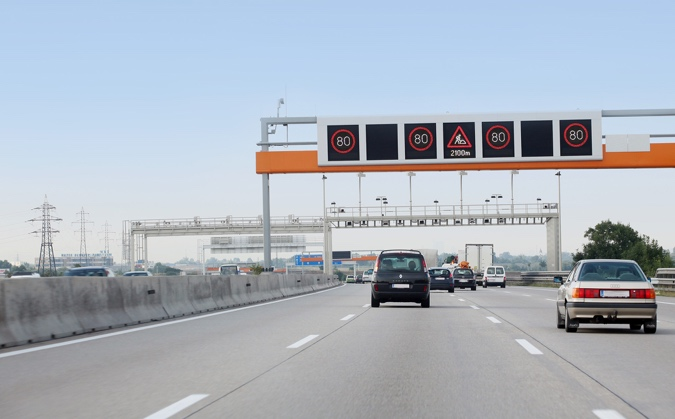
\includegraphics[width=0.9\linewidth]{image/dynamic_signage} \caption{Dynamic signage system in Austria (ASFiNAG, 2019b)}\label{fig:unnamed-chunk-5}
\end{figure}

With respect to the impact on the societal level, a Belgian study, by E. De Pauw et al.~showed a significant decrease (-18 \%) in the number of injury crashes after the introduction of a DSL system (De Pauw et al., 2018). F.G. Habtemichael and L. de Picado Santos (2013) found that a DSL system has the highest safety benefit during highly congested traffic conditions. The operational benefit in turn was the highest during lightly congested traffic conditions. However, the success of DSL is highly dependent on the level of driver compliance (Habtemichael \& de Picado Santos, 2013). Besides the safety aspects, the goal of DSL is to harmonize the traffic flow. Heavy traffic can cause shock waves, which result in longer travel times and large variations in the speeds of the vehicles. The latter again may lead to unsafe situations. By using DSL this phenomenon could be reduced (Hegyi et al., 2005). Traffic flow efficiency can be improved more, when DSL is combined with coordinated ramp metering (Carlson, 2010). Speed limits can also be temporary lowered, due to high emission values. If the emission values combined with the amount of traffic, reach a specific level, the DSL-System responds automatically and lowers the speed limit for a certain time. How high that level is, depends on the local policies (ASFiNAG, 2019c).

\hypertarget{key-stakeholders-8}{%
\subsection*{Key stakeholders}\label{key-stakeholders-8}}
\addcontentsline{toc}{subsection}{Key stakeholders}

\begin{itemize}
\tightlist
\item
  \textbf{Affected}: Motorways users
\item
  \textbf{Responsible}: Motorway Infrastructure Agencies, Technology Providers, Policymakers, State authorities
\end{itemize}

\hypertarget{current-state-of-art-in-research-8}{%
\subsection*{Current state of art in research}\label{current-state-of-art-in-research-8}}
\addcontentsline{toc}{subsection}{Current state of art in research}

Studies show, that in retrospect most DSL implementations in Europe were efficient traffic safety and flow improvement. In the United States the increase in safety was significant as well, but the flow improvement was controversial (Lu \& Shladover, 2014). Hassan et al.~(2012) discovered that during bad weather conditions the combination of Changeable Message Signs (CMS) and DSL was the best way to improve safety. Current research shows that the benefits of DSL systems could be improved by integrating it in a fully connected vehicles (CV) environment (Wu et al., 2020). Currently, research focuses on the integration of C-ITS, to connect the infrastructure to the vehicles. European standards should be developed during the next years (Erhart, 2019).

\hypertarget{current-state-of-art-in-practice-8}{%
\subsection*{Current state of art in practice}\label{current-state-of-art-in-practice-8}}
\addcontentsline{toc}{subsection}{Current state of art in practice}

DSL systems are implemented and used around the world. The used algorithms differ, however. DSL integrated with C-ITS has been implemented in a test environment (Erhart, 2019).
Austrian motorways are managed by the ASFiNAG - currently they have 17 DSL systems in use. That means that about 19 \% of the Austrian Motorway-System are currently equipped by an DSL system (ASFiNAG, 2019a). So, there is potential for expansion. One global player in traffic management is the Austrian company Kapsch TrafficCom. Worldwide they have implemented their systems on more than 3.500 km of motorway (Kapsch TrefficCom). Kapsch TrafficCom's approximately 5,000 employees generated revenues of EUR 738 million in the fiscal year 2018/19.

\hypertarget{relevant-initiatives-in-austria-8}{%
\subsection*{Relevant initiatives in Austria}\label{relevant-initiatives-in-austria-8}}
\addcontentsline{toc}{subsection}{Relevant initiatives in Austria}

\begin{itemize}
\tightlist
\item
  \href{https://www.asfinag.at/verkehrssicherheit/verkehrsmanagement/verkehrssteuerung/}{Asfinag}
\item
  \href{https://blog.asfinag.at/technik-innovation/c-its-vernetzte-autos-intelligenter-verkehr/}{Asifinag blog}
\item
  \href{https://www.kapsch.net/ktc/Portfolio/IMS/Congestion/Highway-Traffic-Management}{kapsch.net}
\item
  \href{https://www.strabag-iss.com/databases/internet/_public/content30.nsf/web30?Openagent\&id=DE-STRABAGISS-DE_verkehrstechnik.html\&men1=3\&men2=5\&sid=351}{strabag-iss.com}
\item
  \href{https://www.pke.at/index.php?id=17\#c117}{pke.at}
\item
  \href{http://www.aigner-stahlbau.at/leistungen/verkehrstechnik/}{aigner-stahlbau.at}
\end{itemize}

\hypertarget{impacts-with-respect-to-sustainable-development-goals-sdgs-8}{%
\subsection*{Impacts with respect to Sustainable Development Goals (SDGs)}\label{impacts-with-respect-to-sustainable-development-goals-sdgs-8}}
\addcontentsline{toc}{subsection}{Impacts with respect to Sustainable Development Goals (SDGs)}

\begin{longtable}[]{@{}ccccc@{}}
\toprule
\begin{minipage}[b]{0.17\columnwidth}\centering
Impact level\strut
\end{minipage} & \begin{minipage}[b]{0.16\columnwidth}\centering
Indicator\strut
\end{minipage} & \begin{minipage}[b]{0.17\columnwidth}\centering
Impact direction\strut
\end{minipage} & \begin{minipage}[b]{0.17\columnwidth}\centering
Goal description and number\strut
\end{minipage} & \begin{minipage}[b]{0.17\columnwidth}\centering
Source\strut
\end{minipage}\tabularnewline
\midrule
\endhead
\begin{minipage}[t]{0.17\columnwidth}\centering
Individual\strut
\end{minipage} & \begin{minipage}[t]{0.16\columnwidth}\centering
Fatal collisions reduced\strut
\end{minipage} & \begin{minipage}[t]{0.17\columnwidth}\centering
\textbf{+}\strut
\end{minipage} & \begin{minipage}[t]{0.17\columnwidth}\centering
Health \& Wellbeing (\emph{3})\strut
\end{minipage} & \begin{minipage}[t]{0.17\columnwidth}\centering
Hegyi et al., 2005\strut
\end{minipage}\tabularnewline
\begin{minipage}[t]{0.17\columnwidth}\centering
Individual\strut
\end{minipage} & \begin{minipage}[t]{0.16\columnwidth}\centering
Travel time reduced\strut
\end{minipage} & \begin{minipage}[t]{0.17\columnwidth}\centering
\textbf{+}\strut
\end{minipage} & \begin{minipage}[t]{0.17\columnwidth}\centering
Environmental sustainability (\emph{7,12,13,15})\strut
\end{minipage} & \begin{minipage}[t]{0.17\columnwidth}\centering
Habtemichael \& de Picado Santos, 2013\strut
\end{minipage}\tabularnewline
\begin{minipage}[t]{0.17\columnwidth}\centering
Systemic\strut
\end{minipage} & \begin{minipage}[t]{0.16\columnwidth}\centering
Fatal collisions reduced\strut
\end{minipage} & \begin{minipage}[t]{0.17\columnwidth}\centering
\textbf{+}\strut
\end{minipage} & \begin{minipage}[t]{0.17\columnwidth}\centering
Health \& Wellbeing (\emph{3})\strut
\end{minipage} & \begin{minipage}[t]{0.17\columnwidth}\centering
Hegyi et al., 2005\strut
\end{minipage}\tabularnewline
\begin{minipage}[t]{0.17\columnwidth}\centering
Systemic\strut
\end{minipage} & \begin{minipage}[t]{0.16\columnwidth}\centering
Annual greenhouse gas emissions decrease\strut
\end{minipage} & \begin{minipage}[t]{0.17\columnwidth}\centering
\textbf{+}\strut
\end{minipage} & \begin{minipage}[t]{0.17\columnwidth}\centering
Environmental sustainability (\emph{7,12-13,15})\strut
\end{minipage} & \begin{minipage}[t]{0.17\columnwidth}\centering
Schimany, 2011\strut
\end{minipage}\tabularnewline
\bottomrule
\end{longtable}

\hypertarget{technology-and-societal-readiness-level-8}{%
\subsection*{Technology and societal readiness level}\label{technology-and-societal-readiness-level-8}}
\addcontentsline{toc}{subsection}{Technology and societal readiness level}

\begin{longtable}[]{@{}cc@{}}
\toprule
TRL & SRL\tabularnewline
\midrule
\endhead
7-9 & 8-9\tabularnewline
\bottomrule
\end{longtable}

\hypertarget{open-questions-8}{%
\subsection*{Open questions}\label{open-questions-8}}
\addcontentsline{toc}{subsection}{Open questions}

\begin{enumerate}
\def\labelenumi{\arabic{enumi}.}
\tightlist
\item
  Which algorithms for DSL are the most efficient ones?
\item
  How can DSL be further developed?
\item
  How can fail-safe operation be improved?
\item
  How can DSL be combined with C-ITS?
\end{enumerate}

\hypertarget{references-8}{%
\subsection*{References}\label{references-8}}
\addcontentsline{toc}{subsection}{References}

\begin{itemize}
\tightlist
\item
  ASFiNAG. (2019a). Handlungsfelder. Retrieved 17th December 2020, from \url{http://verkehrssicherheit.asfinag.at/aktionsprogramme/handlungsfelder/}
\item
  ASFiNAG. (2019b). Verkehrsbeeinflussungsanlagen -- Für mehr Sicherheit: Arten von Verkehrsbeeinflussungsanlagen. Retrieved 11th December 2020, from \url{https://asfinag.azureedge.net/media/1607/vba-fotomontage.jpg}
\item
  ASFiNAG. (2019c). Verkehrsbeeinflussungsanlagen -- Für mehr Sicherheit: Die VBA und der ``Lufthunderter''. Retrieved 3rd December 2020, from \url{https://www.asfinag.at/verkehrssicherheit/verkehrsmanagement/verkehrssteuerung/}
\item
  Carlson, R. C., Papamichail, I., Papageorgiou, M., \& Messmer, A. (2010). Optimal motorway traffic flow control involving variable speed limits and ramp metering. Transportation Science, 44(2), 238-253.
\item
  De Pauw, E., Daniels, S., Franckx, L., \& Mayeres, I. (2018). Safety effects of dynamic speed limits on motorways. Accident Analysis \& Prevention, 114, 83-89.
\item
  Erhart, Jaqueline. (2019). Vernetzte Autos, intelligenter Verkehr: Was C-ITS ist, was es kann und wem es nutzt. Retrieved 17th December 2020, from \url{https://blog.asfinag.at/technik-innovation/c-its-vernetzte-autos-intelligenter-verkehr/}\\
\item
  Habtemichael, F. G., \& de Picado Santos, L. (2013). Safety and Operational Benefits of Variable Speed Limits under Different Traffic Conditions and Driver Compliance Levels. Transportation Research Record, 2386(1), 7--15. \url{https://doi.org/10.3141/2386-02}
\item
  Hassan, H. M., Abdel-Aty, M. A., Choi, K., \& Algadhi, S. A. (2012). Driver behavior and preferences for changeable message signs and variable speed limits in reduced visibility conditions. Journal of Intelligent Transportation Systems, 16(3), 132-146.
\item
  Hegyi, A., De Schutter, B., \& Hellendoorn, J. (2005). Optimal coordination of variable speed limits to suppress shock waves. IEEE Transactions on intelligent transportation systems, 6(1), 102-112.
\item
  Kapsch TrefficCom. Verkehrsmanagement auf Autobahnen. Retrieved 8th January 2021, \url{https://www.kapsch.net/ktc/Portfolio/IMS/Congestion/Highway-Traffic-Management}
\item
  Lu, X.-Y., \& Shladover, S. E. (2014). Review of Variable Speed Limits and Advisories: Theory, Algorithms, and Practice. Transportation Research Record, 2423(1), 15--23. \url{https://doi.org/10.3141/2423-03}
\item
  Mobility and Transport \textbar{} European Commission. (2020). Dynamic speed limits. Retrieved 2nd December 2020, from \url{https://ec.europa.eu/transport/road_safety/specialist/knowledge/speed/new_technologies_new_opportunities/dynamic_speed_limits_en}
\item
  Schimany, H. K. (2011). Blue Globe Foresight.
\item
  Wu, Y., Abdel-Aty, M., Wang, L., \& Rahman, M. S. (2020). Combined connected vehicles and variable speed limit strategies to reduce rear-end crash risk under fog conditions. Journal of Intelligent Transportation Systems, 24(5), 494-513.
\end{itemize}

\hypertarget{adaptive_traffic_control}{%
\section{Adaptive traffic signal control}\label{adaptive_traffic_control}}

\hypertarget{synonyms-8}{%
\subsection*{Synonyms}\label{synonyms-8}}
\addcontentsline{toc}{subsection}{Synonyms}

\emph{Adaptive Traffic Signal Control (ATSC), Traffic Signal Timing (TST), Traffic Signal Control (TSC)}

\hypertarget{definition-9}{%
\subsection*{Definition}\label{definition-9}}
\addcontentsline{toc}{subsection}{Definition}

In the recent years, the increasing population and the urgent need for efficient transport have led to severe traffic problems, especially in urban areas. Congestion mitigation solutions such as optimising the road network and improving basic urban management facilities have been proposed to cope with the pressure caused by the large traffic flow during peak hours. Among all possible methods, the adaptive traffic signal control (ATSC) which combine the intelligence into traffic light control systems has proven to be both, economical and efficient in relieving traffic pressure at congested intersections. With the development of deep learning techniques, ATSC strategies have shown great potential in integrating state-of-the-art intelligent methods (Wang et al., 2021).
Existing traffic light control systems either employ fixed programs without incorporating real-time traffic or take little account of traffic (Casas, 2017). They either set the traffic lights to the same duration every cycle or vary the duration depending on historical information. Some of them take input information from the underground sensors, such as inductive loop detectors, to detect vehicles near the traffic lights. However, such data is processed very crudely to determine the duration of green and red traffic lights. Consequently, they work in some cases (with low efficiency); however, during events such as sports, festivals, weather conditions or a typical high traffic volume scenario, the existing control systems tend to be paralysed.
The recent research paper by Liang et al., 2019 reports that an experienced police officer can efficiently and directly control the intersection by waving signals. Especially, in high traffic volume scenarios, a human operator observes the real-time traffic condition at the intersecting streets and adjusts the duration of the passage time accordingly. The aim of the adaptive traffic signal control is to provide flexibility and efficiency in traffic management comparable to that provided by a human operator through the employment of V2X and Deep Reinforcement learning (Wang et al., 2021).

\hypertarget{key-stakeholders-9}{%
\subsection*{Key stakeholders}\label{key-stakeholders-9}}
\addcontentsline{toc}{subsection}{Key stakeholders}

\begin{itemize}
\tightlist
\item
  \textbf{Affected}: Road drivers, cyclists, pedestrians
\item
  \textbf{Responsible}: Local governments, Local or national road infrastructure provides, car manufacturers
\end{itemize}

\hypertarget{current-state-of-art-in-research-9}{%
\subsection*{Current state of art in research}\label{current-state-of-art-in-research-9}}
\addcontentsline{toc}{subsection}{Current state of art in research}

Existing ATSC methods focus on varying the duration of green or red cycles based on real-time information. Nevertheless, this approach is not optimal because it neglects the impact of the current green and red lights durations on the upcoming traffic. Therefore, ATSC performs better than the fixed duration system but worse than more flexible methods because the optimal phase duration in the last cycles does not perform better in the future considering updated information about complex traffic conditions.

With Deep Learning (DL) methods (which serve as input to the intersection controls), the optimal design of the basic control indices such as green phase duration and phase sequence of the traffic light at an intersection can be considered as an optimal decision-making procedure. Next, the reinforcement learning (RL) is applied to signal control to obtain the best control procedure for a signalised intersection. However, in order to achieve instantaneous data acquisition and transmission with low latency, Cooperative Vehicle Infrastructure System (CVIS) is needed to support inter-vehicle communication and vehicles with roadside infrastructure communication (see \protect\hyperlink{v2x}{V2X section}). Compared to traditional sensor detectors, V2X can collect more accurate traffic data to provide comprehensive information for traffic control, resulting in better RL decision-making (Wang et al., 2021).
Moreover, the analysis of the recent literature for the optimisation of TSC systems, which have been published from January 2015 to January 2020 revealed that only two papers deal with signalised roundabouts. Roundabouts have different traffic dynamics compared to regular intersections. With an increasing use of signalised roundabouts, especially in urban areas, it is believed that TSC for signalised roundabouts is a particular research gap in this area. Although there are studies conducted using real data and real-time control, there are scarce results and/or methods applied or adapted in real life. One of the main challenges for researchers in this field would be to bring these methods to decision makers and implementers.
Moreover, a vast majority of work found on this topic deals with the timing of traffic signals and their impact on average delay and/or emissions. An important part of busy intersections, especially in metropolitan areas, is pedestrian traffic. With the exception of Vilarinho et al., (2017) and Yu et al., (2017), pedestrians and the effects of their behaviour are not modelled in the studies. The same applies for drivers' behaviour. An important research direction would be to analyse the effects of pedestrian and driver behaviour on the models.
Furthermore, the number of studies dealing with autonomous vehicles and technologies is growing rapidly. The most recent studies address the general area of how autonomous vehicles can be introduced safely and/or efficiently and/or environmentally friendly into the traffic flow
(Qadri et al., 2020a).
While learning from trial and error is the key idea in RL, the learning cost of RL for complicated problems might be unacceptable. Therefore, how to learn efficiently (e.g.~from limited data samples, efficient exploration, transfer of learned knowledge) is a critical issue for the application of RL in traffic signal control (Wei et al., 2019).

\hypertarget{current-state-of-art-in-practice-9}{%
\subsection*{Current state of art in practice}\label{current-state-of-art-in-practice-9}}
\addcontentsline{toc}{subsection}{Current state of art in practice}

A number of stakeholders are focusing on the development of adaptive traffic control systems that support a range of smart city traffic applications, such as public transport signal priority (see \protect\hyperlink{public_trans_priority}{PTSP section} for further details), eco-driving support, messaging, intelligent traffic signal control (STSC) and emergency vehicle signal pre-emption (EVSP). Due to these factors and steady advances in sensors, artificial intelligence (AI) and machine learning, the global market for adaptive traffic control systems is forecasted to reach the market value of US\$21.9 billion by the end of 2030.
Governments and city administrations in different regions of the world are looking for new ways to respond to the increasing number of traffic accidents and managing road congestion, which is why adaptive traffic control systems have attracted a lot of interest in recent years as a viable alternative to address the existing challenges (The Sentinel Newspaper, 2021).
There are many options already existing and more are still under development. Currently available adaptive signal control technologies include:

\begin{itemize}
\tightlist
\item
  Split Cycle Offset Optimisation Technique (SCOOT);
\item
  Sydney Coordinated Adaptive Traffic System (SCATS),
\item
  Real Time Hierarchical Optimised Distributed Effective System (RHODES);
\item
  Optimised Policies for Adaptive Control (OPAC) \emph{Virtual Fixed Cycle}
\item
  ACS Lite
\end{itemize}

Real-time control of traffic systems have proven performance record, yet these systems have been deployed in less than 1\% of existing traffic signals in America. The Federal Highway Administration is now working to roll out these technologies to the rest of the country (Curtis, 2017). Further, for example, in Germany the adaptive signal control system has been installed on a 6 km long arterial in Muenster, where it was demonstrated to have positive effect on traffic quality and improve the bus transit by 30\% based on the adopted performance index (Brilon \& Wietholt, 2013).

\hypertarget{relevant-initiatives-in-austria-9}{%
\subsection*{Relevant initiatives in Austria}\label{relevant-initiatives-in-austria-9}}
\addcontentsline{toc}{subsection}{Relevant initiatives in Austria}

\begin{itemize}
\tightlist
\item
  \href{https://www.asfinag.at/road-safety/traffic-management/traffic-control/}{Asfinag}
\item
  \href{https://www.atc.or.at/smart-cities/smart-mobility/urban-traffic-management-solutions/}{ATC}
\end{itemize}

\hypertarget{impacts-with-respect-to-sustainable-development-goals-sdgs-9}{%
\subsection*{Impacts with respect to Sustainable Development Goals (SDGs)}\label{impacts-with-respect-to-sustainable-development-goals-sdgs-9}}
\addcontentsline{toc}{subsection}{Impacts with respect to Sustainable Development Goals (SDGs)}

\begin{longtable}[]{@{}ccccc@{}}
\toprule
\begin{minipage}[b]{0.17\columnwidth}\centering
Impact level\strut
\end{minipage} & \begin{minipage}[b]{0.16\columnwidth}\centering
Indicator\strut
\end{minipage} & \begin{minipage}[b]{0.17\columnwidth}\centering
Impact direction\strut
\end{minipage} & \begin{minipage}[b]{0.17\columnwidth}\centering
Goal description and number\strut
\end{minipage} & \begin{minipage}[b]{0.17\columnwidth}\centering
Source\strut
\end{minipage}\tabularnewline
\midrule
\endhead
\begin{minipage}[t]{0.17\columnwidth}\centering
Systemic\strut
\end{minipage} & \begin{minipage}[t]{0.16\columnwidth}\centering
Scarcity of studies that include the effects of pedestrians behaviour\strut
\end{minipage} & \begin{minipage}[t]{0.17\columnwidth}\centering
\textbf{-}\strut
\end{minipage} & \begin{minipage}[t]{0.17\columnwidth}\centering
Equality (\emph{5,10})\strut
\end{minipage} & \begin{minipage}[t]{0.17\columnwidth}\centering
Qadri et al., 2020b\strut
\end{minipage}\tabularnewline
\begin{minipage}[t]{0.17\columnwidth}\centering
Systemic\strut
\end{minipage} & \begin{minipage}[t]{0.16\columnwidth}\centering
Decrease in congestion at the intersections\strut
\end{minipage} & \begin{minipage}[t]{0.17\columnwidth}\centering
\textbf{+}\strut
\end{minipage} & \begin{minipage}[t]{0.17\columnwidth}\centering
Sustainable economic development (\emph{8,11})\strut
\end{minipage} & \begin{minipage}[t]{0.17\columnwidth}\centering
Wang et al., 2021\strut
\end{minipage}\tabularnewline
\begin{minipage}[t]{0.17\columnwidth}\centering
Systemic\strut
\end{minipage} & \begin{minipage}[t]{0.16\columnwidth}\centering
Progress in the use of RL algorithms and V2X technologies\strut
\end{minipage} & \begin{minipage}[t]{0.17\columnwidth}\centering
\textbf{+}\strut
\end{minipage} & \begin{minipage}[t]{0.17\columnwidth}\centering
Innovation \& Infrastructure (\emph{9})\strut
\end{minipage} & \begin{minipage}[t]{0.17\columnwidth}\centering
Wang et al., 2021\strut
\end{minipage}\tabularnewline
\bottomrule
\end{longtable}

\hypertarget{technology-and-societal-readiness-level-9}{%
\subsection*{Technology and societal readiness level}\label{technology-and-societal-readiness-level-9}}
\addcontentsline{toc}{subsection}{Technology and societal readiness level}

\begin{longtable}[]{@{}cc@{}}
\toprule
TRL & SRL\tabularnewline
\midrule
\endhead
7-9 & 7-8\tabularnewline
\bottomrule
\end{longtable}

\hypertarget{open-questions-9}{%
\subsection*{Open questions}\label{open-questions-9}}
\addcontentsline{toc}{subsection}{Open questions}

\begin{enumerate}
\def\labelenumi{\arabic{enumi}.}
\tightlist
\item
  How can ATSC for signalised roundabouts be designed, developed and implemented?
\item
  How can pedestrian movement be included to a larger extent into the algorithms of ATSC?
\item
  How can reinforcement learning algorithms learn efficiently from limited data samples for the purpose traffic signal control?
\end{enumerate}

\hypertarget{further-links-7}{%
\subsection*{Further links}\label{further-links-7}}
\addcontentsline{toc}{subsection}{Further links}

\begin{itemize}
\tightlist
\item
  \href{https://www.rapidflowtech.com/surtrac}{rapidflowtech.com}
\item
  \href{https://www.fhwa.dot.gov/innovation/everydaycounts/edc-1/asct.cfm}{fhwa.dot.gov}
\end{itemize}

\hypertarget{references-9}{%
\subsection*{References}\label{references-9}}
\addcontentsline{toc}{subsection}{References}

\begin{itemize}
\tightlist
\item
  Brilon, W., \& Wietholt, T. (2013). Experiences with adaptive signal control in Germany. Transportation research record, 2356(1), 9-16.
\item
  Casas, N. (2017). Deep deterministic policy gradient for urban traffic light control. ArXiv, 1--12.
\item
  Curtis, E. (2017, September 8). EDC-1: Adaptive Signal Control Technology \textbar{} Federal Highway Administration. \url{https://www.fhwa.dot.gov/innovation/everydaycounts/edc-1/asct.cfm}
\item
  Liang, X., Du, X., Wang, G., \& Han, Z. (2019). A Deep Reinforcement Learning Network for Traffic Light Cycle Control. IEEE Transactions on Vehicular Technology, 68(2), 1243--1253. \url{https://doi.org/10.1109/TVT.2018.2890726}
\item
  Qadri, S. S. S. M., Gökçe, M. A., \& Öner, E. (2020a). State-of-art review of traffic signal control methods: challenges and opportunities. European Transport Research Review, 12(1), 55. \url{https://doi.org/10.1186/s12544-020-00439-1}
\item
  Qadri, S. S. S. M., Gökçe, M. A., \& Öner, E. (2020b). State-of-art review of traffic signal control methods: challenges and opportunities. European Transport Research Review, 12(1), 1--23. \url{https://doi.org/10.1186/s12544-020-00439-1}
\item
  The Sentinel Newspaper. (2021, March 3). Adaptive Traffic Control System Market to reach US\$ 21.9 Bn by 2030 -- KSU \textbar{} The Sentinel Newspaper. \url{https://ksusentinel.com/2021/03/03/adaptive-traffic-control-system-market-to-reach-us-21-9-bn-by-2030/}
\item
  Vilarinho, C., Tavares, J. P., \& Rossetti, R. J. F. (2017). Intelligent Traffic Lights: Green Time Period Negotiaton. Transportation Research Procedia, 22, 325--334. \url{https://doi.org/https://doi.org/10.1016/j.trpro.2017.03.039}
\item
  Wang, T., Cao, J., \& Hussain, A. (2021). Adaptive Traffic Signal Control for large-scale scenario with Cooperative Group-based Multi-agent reinforcement learning. Transportation Research Part C: Emerging Technologies, 125(February), 103046. \url{https://doi.org/10.1016/j.trc.2021.103046}
\item
  Wei, H., Zheng, G., Gayah, V., \& Li, Z. (2019). A survey on traffic signal control methods. ArXiv, 1(1).
\item
  Yu, C., Ma, W., Han, K., \& Yang, X. (2017). Optimization of vehicle and pedestrian signals at isolated intersections. Transportation Research Part B: Methodological, 98, 135--153. \url{https://doi.org/https://doi.org/10.1016/j.trb.2016.12.015}
\end{itemize}

\hypertarget{p_g_fleet_management}{%
\section{Passengers and goods fleet management}\label{p_g_fleet_management}}

\hypertarget{urban_access}{%
\section{Urban access management}\label{urban_access}}

\hypertarget{synonyms-9}{%
\subsection*{Synonyms}\label{synonyms-9}}
\addcontentsline{toc}{subsection}{Synonyms}

\emph{Access Regulation Schemes (ARS), Urban Vehicle Access Regulations (UVARs), Low Emission Zones (LEZ), Access Restrictions, Traffic Restrictions, Limited Traffic Zones, Permit Schemes}

\hypertarget{definition-10}{%
\subsection*{Definition}\label{definition-10}}
\addcontentsline{toc}{subsection}{Definition}

Urban Access Management can be seen as regulations, restrictions or bans, for traffic entering cities. Factors like congestion, air pollution, traffic noise or damage to historic buildings are influencing the liveability of cities negatively. Therefore, many cities have been introducing Access Regulation Schemes (ARS) with the goal of less vehicles entering the particular city or area. Implementing a pedestrian zone, is the simplest type of ARS and can improve the attractiveness of tourist attractions or shopping streets significantly (Sadler Consultants Europe GmbH, n.d. c). ARS can be differentiated by vehicle type, vehicle weight, by type of trip (e.g.~delivery), by driver (e.g.~residents or access), or applies to all vehicles (Sadler Consultants Europe GmbH, n.d. c). Furthermore, ARS can be static or dynamic, depending, for example, on the time of the day or air pollution levels. A list below provides examples of current measures used in the urban areas:

\begin{itemize}
\tightlist
\item
  Low Emission Zones (LEZ)
\item
  Limited Access Zones
\item
  Urban Toll Schemes / Congestion Charging (CS)
\item
  Emergency Air Pollution Schemes
\item
  Zero Emission Zones (ZEZ)
\item
  Other Access Regulations (like Limited Traffic Zones, Through traffic bans, `Superblocks´ etc.)
\item
  Smaller Regulations / Restrictions (like school streets or shared spaces) (Sandler Consultants Europe GmbH, n.d. d).
\end{itemize}

Solutions for ARS can be enforced by physical barriers or cameras, based on automatic number plate recognition (ANPR) systems and/or dedicated short-range communication (DSRC) technology, using on-board units (OBUs) (Kapsch TrafficCom., n.d. b) or by police or local authority officers (Sadler Consultants Europe GmbH, n.d. c).

The impact of Urban Vehicle Access Regulations differs according the implemented schemes, but several common goals are addressed:
- Air quality improvement
- Traffic congestion reduction
- Urban landscape preservation (historical town centres)
- Climate change mitigation
- Quality of life
- Noise mitigation
- Road safety
- Raising revenues (Sandler Consultants Europe GmbH, n.d. d).

In Austria, several cities and regions have implemented Low Emission Zones (LEZ) for lorries. For example, the city of Salzburg has Access Regulations (AR) for the city centre in place, so only vehicles with a specific reason (delivery or police) are allowed to enter. On the other hand, Tirol introduces occasionally traffic bans during the summer months (Sandler Consultants Europe GmbH, n.d. a). While, the city of Vienna aims at implementing a traffic-calmed city centre by 2022 (Stadt Wien, 2020).

\hypertarget{key-stakeholders-10}{%
\subsection*{Key stakeholders}\label{key-stakeholders-10}}
\addcontentsline{toc}{subsection}{Key stakeholders}

\begin{itemize}
\tightlist
\item
  \textbf{Affected}: Car Users -- especially users of old or high polluting cars, truck drivers, Shippers/producers, Wholesalers, Logistics providers, Retailers, Consumers, Citizens, Authorities
\item
  \textbf{Responsible}: Municipalities, Road Operators, Urban Traffic Management, Authorities
\end{itemize}

\hypertarget{current-state-of-art-in-research-10}{%
\subsection*{Current state of art in research}\label{current-state-of-art-in-research-10}}
\addcontentsline{toc}{subsection}{Current state of art in research}

Current research addresses the evaluation of UVAR implementations and identifies their positive and negative effects. For example, Lopez (2018) found that Urban Consolidation Centres (UCCs), Cargo Bikes (CBs) and Off-hour Deliveries (OHDs) are the three preferred types of solutions to assist in mitigating unwanted side-effects of UVARs on the logistic sector. Further, current research focuses on the sustainable urban planning in cites affected by mass tourism (García Hernández, 2019; Nolasco‐Cirugeda, 2020). Additionally, most recent area of research deals with geofencing that aims at creating digital zones defined on a map, with specific rules, that can be transmitted to the vehicles (Arnesen et al., 2020).

\hypertarget{current-state-of-art-in-practice-10}{%
\subsection*{Current state of art in practice}\label{current-state-of-art-in-practice-10}}
\addcontentsline{toc}{subsection}{Current state of art in practice}

According to Lopez (2018) there are the two preferred UVAR schemes: Low Emission Zones (LEZ) and Congestion Charging (CC). The implementation of these schemes is widely spread within Europe but follows different approaches. Lopez (2018) identified two dominant LEZ enforcement models, first visual surveillance using windscreen stickers and second, cameras with ANPR technology. Furthermore it is argued that \emph{``It is very important to consider that the degree of impact of each measure not only varies from city to city but also depends on the presence of a mix of access regulations``} (Lopez, 2018).

\hypertarget{relevant-initiatives-in-austria-10}{%
\subsection*{Relevant initiatives in Austria}\label{relevant-initiatives-in-austria-10}}
\addcontentsline{toc}{subsection}{Relevant initiatives in Austria}

\begin{itemize}
\tightlist
\item
  \href{https://www.ris.bka.gv.at/GeltendeFassung.wxe?Abfrage=LrW\&Gesetzesnummer=20000270}{ris.bka.gv.at}
\item
  \href{https://www.wien.gv.at/ma22-lgb/luftgi.htm}{wien.gv.at}
\item
  \href{https://www.kapsch.net/ktc/its-solutions/urban-access-management/access-restriction/}{kapsch.net}
\end{itemize}

\hypertarget{impacts-with-respect-to-sustainable-development-goals-sdgs-10}{%
\subsection*{Impacts with respect to Sustainable Development Goals (SDGs)}\label{impacts-with-respect-to-sustainable-development-goals-sdgs-10}}
\addcontentsline{toc}{subsection}{Impacts with respect to Sustainable Development Goals (SDGs)}

\begin{longtable}[]{@{}ccccc@{}}
\toprule
\begin{minipage}[b]{0.17\columnwidth}\centering
Impact level\strut
\end{minipage} & \begin{minipage}[b]{0.16\columnwidth}\centering
Indicator\strut
\end{minipage} & \begin{minipage}[b]{0.17\columnwidth}\centering
Impact direction\strut
\end{minipage} & \begin{minipage}[b]{0.17\columnwidth}\centering
Goal description and number\strut
\end{minipage} & \begin{minipage}[b]{0.17\columnwidth}\centering
Source\strut
\end{minipage}\tabularnewline
\midrule
\endhead
\begin{minipage}[t]{0.17\columnwidth}\centering
Individual\strut
\end{minipage} & \begin{minipage}[t]{0.16\columnwidth}\centering
Noise \& pollution reduced\strut
\end{minipage} & \begin{minipage}[t]{0.17\columnwidth}\centering
\textbf{+}\strut
\end{minipage} & \begin{minipage}[t]{0.17\columnwidth}\centering
Health \& Wellbeing (\emph{3})\strut
\end{minipage} & \begin{minipage}[t]{0.17\columnwidth}\centering
Sandler Consultants Europe GmbH, n.d. b\strut
\end{minipage}\tabularnewline
\begin{minipage}[t]{0.17\columnwidth}\centering
Individual\strut
\end{minipage} & \begin{minipage}[t]{0.16\columnwidth}\centering
Travel time \& congestion reduced\strut
\end{minipage} & \begin{minipage}[t]{0.17\columnwidth}\centering
\textbf{+}\strut
\end{minipage} & \begin{minipage}[t]{0.17\columnwidth}\centering
Sustainable economic development (\emph{8,11})\strut
\end{minipage} & \begin{minipage}[t]{0.17\columnwidth}\centering
Sandler Consultants Europe GmbH, n.d. b\strut
\end{minipage}\tabularnewline
\begin{minipage}[t]{0.17\columnwidth}\centering
Systemic\strut
\end{minipage} & \begin{minipage}[t]{0.16\columnwidth}\centering
Road safety increased\strut
\end{minipage} & \begin{minipage}[t]{0.17\columnwidth}\centering
\textbf{+}\strut
\end{minipage} & \begin{minipage}[t]{0.17\columnwidth}\centering
Health \& Wellbeing (\emph{3})\strut
\end{minipage} & \begin{minipage}[t]{0.17\columnwidth}\centering
Sandler Consultants Europe GmbH, n.d. b\strut
\end{minipage}\tabularnewline
\begin{minipage}[t]{0.17\columnwidth}\centering
Systemic\strut
\end{minipage} & \begin{minipage}[t]{0.16\columnwidth}\centering
Space for sustainable transport users increased\strut
\end{minipage} & \begin{minipage}[t]{0.17\columnwidth}\centering
\textbf{+}\strut
\end{minipage} & \begin{minipage}[t]{0.17\columnwidth}\centering
Equality (\emph{5,10})\strut
\end{minipage} & \begin{minipage}[t]{0.17\columnwidth}\centering
Sandler Consultants Europe GmbH, n.d. d\strut
\end{minipage}\tabularnewline
\begin{minipage}[t]{0.17\columnwidth}\centering
Systemic\strut
\end{minipage} & \begin{minipage}[t]{0.16\columnwidth}\centering
Air quality improved\strut
\end{minipage} & \begin{minipage}[t]{0.17\columnwidth}\centering
\textbf{+}\strut
\end{minipage} & \begin{minipage}[t]{0.17\columnwidth}\centering
Environmental sustainability (\emph{7,12,13,15})\strut
\end{minipage} & \begin{minipage}[t]{0.17\columnwidth}\centering
Sandler Consultants Europe GmbH, n.d. d\strut
\end{minipage}\tabularnewline
\begin{minipage}[t]{0.17\columnwidth}\centering
Systemic\strut
\end{minipage} & \begin{minipage}[t]{0.16\columnwidth}\centering
Congestion reduced, revenues increased\strut
\end{minipage} & \begin{minipage}[t]{0.17\columnwidth}\centering
\textbf{+}\strut
\end{minipage} & \begin{minipage}[t]{0.17\columnwidth}\centering
Sustainable economic development (\emph{8,11})\strut
\end{minipage} & \begin{minipage}[t]{0.17\columnwidth}\centering
Sandler Consultants Europe GmbH, n.d. b\strut
\end{minipage}\tabularnewline
\begin{minipage}[t]{0.17\columnwidth}\centering
Systemic\strut
\end{minipage} & \begin{minipage}[t]{0.16\columnwidth}\centering
Urban landscape preservation\strut
\end{minipage} & \begin{minipage}[t]{0.17\columnwidth}\centering
\textbf{+}\strut
\end{minipage} & \begin{minipage}[t]{0.17\columnwidth}\centering
Innovation \& Infrastructure (\emph{9})\strut
\end{minipage} & \begin{minipage}[t]{0.17\columnwidth}\centering
Sandler Consultants Europe GmbH, n.d. b\strut
\end{minipage}\tabularnewline
\bottomrule
\end{longtable}

\hypertarget{technology-and-societal-readiness-level-10}{%
\subsection*{Technology and societal readiness level}\label{technology-and-societal-readiness-level-10}}
\addcontentsline{toc}{subsection}{Technology and societal readiness level}

\begin{longtable}[]{@{}cc@{}}
\toprule
TRL & SRL\tabularnewline
\midrule
\endhead
7-9 & 7-9\tabularnewline
\bottomrule
\end{longtable}

\hypertarget{open-questions-10}{%
\subsection*{Open questions}\label{open-questions-10}}
\addcontentsline{toc}{subsection}{Open questions}

\begin{enumerate}
\def\labelenumi{\arabic{enumi}.}
\tightlist
\item
  What effect will autonomous vehicles have on Urban Access Management?
\item
  How can geofencing be implemented on a wider scale and what are the barriers?
\item
  What standards would be useful to aggregate, to support affected stakeholders?
\item
  How can Urban Access Management engage with the Internet of Things (IoT)?
\end{enumerate}

\hypertarget{further-links-8}{%
\subsection*{Further links}\label{further-links-8}}
\addcontentsline{toc}{subsection}{Further links}

\begin{itemize}
\tightlist
\item
  \href{https://urbanaccessregulations.eu/urban-access-regulations/what-are-urban-access-regulations}{urbanaccessregulations.eu-1}
\item
  \href{https://urbanaccessregulations.eu/countries-mainmenu-147/austria-mainmenu-78/wien-vienna-emergency-scheme}{urbanaccessregulations.eu-2}
\end{itemize}

\hypertarget{references-10}{%
\subsection*{References}\label{references-10}}
\addcontentsline{toc}{subsection}{References}

\begin{itemize}
\tightlist
\item
  Arnesen, P., Seter, H., Foss, T., Dahl, E., Lillestøl, P. J., \& Jenssen, G. (2020). Geofencing for smart urban mobility. Summarizing the main findings of work package 2: Pilot Design and work package 3: Piloting.
\item
  García Hernández, M., Ivars-Baidal, J., \& Mendoza de Miguel, S. (2019). Overtourism in urban destinations: the myth of smart solutions.
\item
  Kapsch TrafficCom. (n.d. a). Access management \textbar{} Kapsch. Retrieved January 27, 2021, from \url{https://www.kapsch.net/ktc/Portfolio/IMS/Smart-Urban-Mobility/Access-Management}
\item
  Kapsch TrafficCom. (n.d. b). Limited Access Zone \textbar{} Kapsch. Retrieved January 27, 2021, from \url{https://www.kapsch.net/ktc/its-solutions/urban-access-management/access-restriction/}
\item
  Lopez, O. N. (2018). Urban vehicle access regulations. In Sustainable Freight Transport (pp.~139-163). Springer, Cham.
\item
  Nolasco‐Cirugeda, A., Martí, P., \& Ponce, G. (2020). Keeping mass tourism destinations sustainable via urban design: The case of Benidorm. Sustainable Development, 28(5), 1289-1303.
\item
  Sandler Consultants Europe GmbH. (n.d. a). Austria. Retrieved February 1, 2021, from \url{https://urbanaccessregulations.eu/countries-mainmenu-147/austria-mainmenu-78}
\item
  Sandler Consultants Europe GmbH. (n.d. b). Overview of website. Retrieved February 1, 2021, from \url{https://urbanaccessregulations.eu/userhome/general-overview\#Why\%20Access\%20\%20Regulations}\\
\item
  Sadler Consultants Europe GmbH. (n.d. c). Urban Access Regulations in Europe. Retrieved 26th January 2021, from \url{https://urbanaccessregulations.eu/about-us}
\item
  Sandler Consultants Europe GmbH. (n.d. d). What are Access Regulations? Retrieved February 1, 2021, from \url{https://urbanaccessregulations.eu/userhome/what-are-access-regulations-uvars-or-urban-vehicle-access-regulations}
\item
  Stadt Wien. (2020). Smarte Mobilität - Die Fortschrittskoalition für Wien. Retrieved February 1, 2021, from \url{https://www.wien.gv.at/regierungsabkommen2020/smart-city-wien/smarte-mobilitat/}
\end{itemize}

\hypertarget{digital}{%
\chapter{Digital road infrastructure and connectivity}\label{digital}}

\hypertarget{v2x}{%
\section{Vehicle to everything communication}\label{v2x}}

\hypertarget{synonyms-10}{%
\subsection*{Synonyms}\label{synonyms-10}}
\addcontentsline{toc}{subsection}{Synonyms}

\emph{Connected Vehicle (CV), Connected Vehicle technologies (CVT), Vehicle-to-x (car and infrastructure) (C2x/V2x), Cooperative Intelligent Transport Systems (C-ITS), Cellular-V2X technology (C-V2X)}

\hypertarget{definition-11}{%
\subsection*{Definition}\label{definition-11}}
\addcontentsline{toc}{subsection}{Definition}

Through Intelligent Transportation Systems (ITS), various Connected Vehicle (CV) technologies have been developed in recent years to contribute to safer roads through cooperative situational awareness and hazard avoidance. Two main types of communication have been proposed: vehicle-to-vehicle (V2V) and vehicle-to-infrastructure (V2I) communication (Outay et al., 2019).
C2X (car to everything) or more broadly V2X (vehicle to everything) is the new technology that enables both communication between vehicles (car-to-car) and information exchange with infrastructure (car-to-infrastructure) (ADAC, 2021).
V2V offers benefits in terms of increased safety, as it can prevent accidents by allowing a vehicle to exchange real-time information about speed, location and direction with other vehicles in the surrounding area. In addition to their safety applications, V2V and V2I communications can potentially help reduce fuel consumption and emissions due to the fact that excessive pollutant emissions are often associated with heavy braking, changing traveling speeds and acceleration/deceleration, especially at signalised intersections. In the context of smart cities, many researchers are exploring the potential use of connected vehicles to support eco-friendly driving by reducing CO\textsubscript{2} emissions. This is often achieved through vehicle-to-vehicle (V2V) and vehicle-to-roadside unit RSU (V2I) inter-connectivity to harmonise vehicle speeds by maintaining traffic flow and reducing unnecessary stops and starts (Outay et al., 2019).
In terms of the communication technology used for V2X, according to Dey et al.~(2016) Dedicated Short Range Communication (DSRC) was considered the primary option for CVT security applications in 2016. However, the use of other radio technologies such as Wi-Fi, LTE or WiMAX enables communication with greater range and provides higher throughput requirements that could not be supported by DSRC alone. In addition, the use of other radio technologies potentially reduces the need for costly DSRC infrastructure.

\hypertarget{key-stakeholders-11}{%
\subsection*{Key stakeholders}\label{key-stakeholders-11}}
\addcontentsline{toc}{subsection}{Key stakeholders}

\begin{itemize}
\tightlist
\item
  \textbf{Affected}: Car drivers, Insurers
\item
  \textbf{Responsible}: National Governments, Private Companies, Car Manufacturers, Infrastructure operators
\end{itemize}

\hypertarget{current-state-of-art-in-research-11}{%
\subsection*{Current state of art in research}\label{current-state-of-art-in-research-11}}
\addcontentsline{toc}{subsection}{Current state of art in research}

Many research papers focus on the technical performance of this technology, the comparison of V2V with V2I and the mixing of V2V vehicles with non-V2V equipped vehicles. As in 2019, the idea of combining V2V and V2I communications into a hybrid V2X alert system has already became reality (Outay et al., 2019).
Moreover, research is conducted on the comparison of available communication technology to ensure the fastest, most efficient and error-free solution. Currently, there are two possibilities under discussion for Car2X communication. Firstly, the IEEE 802.11p Dedicated Short Range Communication (DSRC) and secondly, the Cellular-V2X technology (C-V2X). The former is based on the IEEE 802.11 WiFi standard, while C-V2X is based on 4G LTE, with a roadmap towards 5G C-V-to-X. While China and USA primarily rely on C-V2X, Europe is still undecided as to whether car networking should take place via pWLAN or via C-V2X. This creates an international confusion of languages. As a result, vehicles may not be able to communicate without errors because they use different languages (Köllner, 2020).
IEEE 802.11p is technically very advanced and operates with minimal latencies. But the advantage of 5GAA technology is that 5G is to be introduced globally on a massive scale in the near future and the fast-mobile radio standard will be in the car anyway, if only to transmit the huge amounts of data generated by autonomous driving. Moreover, in a dense 5G network, far fewer of the 5.9 GHz units needed for direct communication have to be integrated into the infrastructure than with the 802.11p solution. Some of the tasks of these units will then be taken over by the 5G network (Knecht, 2018).

\hypertarget{current-state-of-art-in-practice-11}{%
\subsection*{Current state of art in practice}\label{current-state-of-art-in-practice-11}}
\addcontentsline{toc}{subsection}{Current state of art in practice}

So far, C2X is only available from some German manufacturers. Only Ford models, the Volkswagen Golf 8 and all Volvo models always have C2X on board as standard. This is desirable from the point of view of consumer protection, because more cars are equipped with C2X, more accurate this system is in preventing accidents. Again, only Golf and Volvo models have C2X free of charge after purchase. All other manufacturers charge money for C2X after one to three years. Moreover, C2X is never available on its own, but only in a package with other Connect services that do not necessarily have anything to do with road safety (ADAC, 2021).
Several important technical specificities should be considered for V2V communication:

\begin{itemize}
\tightlist
\item
  The time it takes for a warning to reach another car. This varies greatly between manufacturers, ranging from 0.1 seconds to 2 minutes - with the latter value being far too slow for many situations (e.g.~the end of a traffic jam behind a bend).
\item
  Various transmission techniques currently prevent cars from all manufacturers from warning each other.
\item
  With many manufacturers, warnings cannot be passed on if the car is in a cellular network dead zone.
\item
  The number of dangerous situations that are warned about varies from manufacturer to manufacturer.
\end{itemize}

In the table below, we compare how the warnings specification differ between three car manufactures:

\begin{longtable}[]{@{}ccc@{}}
\toprule
\begin{minipage}[b]{0.30\columnwidth}\centering
Audi\strut
\end{minipage} & \begin{minipage}[b]{0.30\columnwidth}\centering
Ford\strut
\end{minipage} & \begin{minipage}[b]{0.30\columnwidth}\centering
Mercedes\strut
\end{minipage}\tabularnewline
\midrule
\endhead
\begin{minipage}[t]{0.30\columnwidth}\centering
broken-down vehicles\strut
\end{minipage} & \begin{minipage}[t]{0.30\columnwidth}\centering
broken-down vehicles\strut
\end{minipage} & \begin{minipage}[t]{0.30\columnwidth}\centering
breakdown\strut
\end{minipage}\tabularnewline
\begin{minipage}[t]{0.30\columnwidth}\centering
accidents\strut
\end{minipage} & \begin{minipage}[t]{0.30\columnwidth}\centering
general traffic warning\strut
\end{minipage} & \begin{minipage}[t]{0.30\columnwidth}\centering
accident\strut
\end{minipage}\tabularnewline
\begin{minipage}[t]{0.30\columnwidth}\centering
end of traffic jam\strut
\end{minipage} & \begin{minipage}[t]{0.30\columnwidth}\centering
end of traffic jam\strut
\end{minipage} & \begin{minipage}[t]{0.30\columnwidth}\centering
-\strut
\end{minipage}\tabularnewline
\begin{minipage}[t]{0.30\columnwidth}\centering
fog, black ice\strut
\end{minipage} & \begin{minipage}[t]{0.30\columnwidth}\centering
dangerous road conditions (icy, heavy rain, oil, etc.)\strut
\end{minipage} & \begin{minipage}[t]{0.30\columnwidth}\centering
heavy rain, fog,crosswind and icy roads\strut
\end{minipage}\tabularnewline
\begin{minipage}[t]{0.30\columnwidth}\centering
online traffic sign information\strut
\end{minipage} & \begin{minipage}[t]{0.30\columnwidth}\centering
-\strut
\end{minipage} & \begin{minipage}[t]{0.30\columnwidth}\centering
hazard warning lights switched on\strut
\end{minipage}\tabularnewline
\begin{minipage}[t]{0.30\columnwidth}\centering
-\strut
\end{minipage} & \begin{minipage}[t]{0.30\columnwidth}\centering
-\strut
\end{minipage} & \begin{minipage}[t]{0.30\columnwidth}\centering
additional hazard manually reported by the driver through the navigation menu\strut
\end{minipage}\tabularnewline
\begin{minipage}[t]{0.30\columnwidth}\centering
display of the probability of free parking spaces along roads incl.~additional information such as prices\strut
\end{minipage} & \begin{minipage}[t]{0.30\columnwidth}\centering
-\strut
\end{minipage} & \begin{minipage}[t]{0.30\columnwidth}\centering
-\strut
\end{minipage}\tabularnewline
\begin{minipage}[t]{0.30\columnwidth}\centering
speed recommendation to reach the next traffic light in a green phase\strut
\end{minipage} & \begin{minipage}[t]{0.30\columnwidth}\centering
-\strut
\end{minipage} & \begin{minipage}[t]{0.30\columnwidth}\centering
-\strut
\end{minipage}\tabularnewline
\begin{minipage}[t]{0.30\columnwidth}\centering
-\strut
\end{minipage} & \begin{minipage}[t]{0.30\columnwidth}\centering
road works\strut
\end{minipage} & \begin{minipage}[t]{0.30\columnwidth}\centering
-\strut
\end{minipage}\tabularnewline
\begin{minipage}[t]{0.30\columnwidth}\centering
-\strut
\end{minipage} & \begin{minipage}[t]{0.30\columnwidth}\centering
objects, animas, people on the road\strut
\end{minipage} & \begin{minipage}[t]{0.30\columnwidth}\centering
-\strut
\end{minipage}\tabularnewline
\begin{minipage}[t]{0.30\columnwidth}\centering
-\strut
\end{minipage} & \begin{minipage}[t]{0.30\columnwidth}\centering
wrong-way drivers\strut
\end{minipage} & \begin{minipage}[t]{0.30\columnwidth}\centering
-\strut
\end{minipage}\tabularnewline
\bottomrule
\end{longtable}

Moreover, the ADAC's recommendations to the manufacturers are the following (ADAC, 2021):

\begin{itemize}
\tightlist
\item
  The manufacturers should quickly agree on a transmission technology.
\item
  C2X should quickly become standard equipment
\item
  Safety-relevant C2X functions should not cause any follow-up costs
\end{itemize}

A basis for cooperative systems is currently being established in Europe. The procedures for testing under real traffic conditions are being defined and coordinated among the partners involved. A large part of the technical solutions for data communication is standardised. The non-technical aspects (e.g.~organisational structures, safety concept) are currently being worked out in preparation for the market launch in a public-private partnership.
On this basis, German, Dutch and Austrian road operators, together with partners from industry, are starting the step-by-step introduction of cooperative systems in Europe within the framework of the C-ITS corridor from Rotterdam to Frankfurt am Main and Vienna
(Cooperative ITS Corridor, no date).
In Austria, with the award of a comprehensive framework contract, ASFINAG has now become the first infrastructure provider in Europe to reach a further milestone in networking vehicles and roads. The total volume of the framework contract is 14.5 million euros. This will make it possible to equip the entire motorway network in Austria with C-ITS in the coming years.The equipment, which will be installed step by step along the motorways starting in November, includes up to 525 so-called road units as well as a control centre. The first C-ITS services for hazard warning are expected to go into operation within the next 16 months. Further expansion will focus on the support of automated driving and networked traffic management. The C-ITS equipment is part of the digitalisation of the road infrastructure and is funded by the Climate and Energy Fund and the EU (Močnik, 2020).

\hypertarget{relevant-initiatives-in-austria-11}{%
\subsection*{Relevant initiatives in Austria}\label{relevant-initiatives-in-austria-11}}
\addcontentsline{toc}{subsection}{Relevant initiatives in Austria}

\begin{itemize}
\tightlist
\item
  \href{https://infothek.bmk.gv.at/fahrer-assistenzsysteme-verkehrssicherheit-vernetzung/}{infothek.bmk.gv.at}
\item
  \href{https://c-its-korridor.de/?menuId=1\&sp=en}{c-its-korridor.de}
\item
  \href{https://www.asfinag.at/ueber-uns/newsroom/pressemeldungen/2020/wlan-ausbau-cooperative-intelligent-transport-systems/}{asfinag.at}
\item
  \href{https://www.kununu.com/de/automotive-safety-technologies/news/car2x-projekt-in-oesterreich-praesentiert}{kununu.com}
\item
  \href{https://www.hitech.at/mobilitaet/wohin-geht-die-fahrt}{hitech.at}
\end{itemize}

\hypertarget{impacts-with-respect-to-sustainable-development-goals-sdgs-11}{%
\subsection*{Impacts with respect to Sustainable Development Goals (SDGs)}\label{impacts-with-respect-to-sustainable-development-goals-sdgs-11}}
\addcontentsline{toc}{subsection}{Impacts with respect to Sustainable Development Goals (SDGs)}

\begin{longtable}[]{@{}ccccc@{}}
\toprule
\begin{minipage}[b]{0.17\columnwidth}\centering
Impact level\strut
\end{minipage} & \begin{minipage}[b]{0.16\columnwidth}\centering
Indicator\strut
\end{minipage} & \begin{minipage}[b]{0.17\columnwidth}\centering
Impact direction\strut
\end{minipage} & \begin{minipage}[b]{0.17\columnwidth}\centering
Goal description and number\strut
\end{minipage} & \begin{minipage}[b]{0.17\columnwidth}\centering
Source\strut
\end{minipage}\tabularnewline
\midrule
\endhead
\begin{minipage}[t]{0.17\columnwidth}\centering
Individual\strut
\end{minipage} & \begin{minipage}[t]{0.16\columnwidth}\centering
Improvement of road safety\strut
\end{minipage} & \begin{minipage}[t]{0.17\columnwidth}\centering
\textbf{+}\strut
\end{minipage} & \begin{minipage}[t]{0.17\columnwidth}\centering
Health \& Wellbeing (\emph{3})\strut
\end{minipage} & \begin{minipage}[t]{0.17\columnwidth}\centering
Filippi et al., 2016\strut
\end{minipage}\tabularnewline
\begin{minipage}[t]{0.17\columnwidth}\centering
Individual\strut
\end{minipage} & \begin{minipage}[t]{0.16\columnwidth}\centering
V2X communications will come at no cost to the end user\strut
\end{minipage} & \begin{minipage}[t]{0.17\columnwidth}\centering
\textbf{+}\strut
\end{minipage} & \begin{minipage}[t]{0.17\columnwidth}\centering
Sustainable economic development (\emph{8,11})\strut
\end{minipage} & \begin{minipage}[t]{0.17\columnwidth}\centering
Hainen et al., 2019\strut
\end{minipage}\tabularnewline
\begin{minipage}[t]{0.17\columnwidth}\centering
Systemic\strut
\end{minipage} & \begin{minipage}[t]{0.16\columnwidth}\centering
Emissions reduced\strut
\end{minipage} & \begin{minipage}[t]{0.17\columnwidth}\centering
\textbf{+}\strut
\end{minipage} & \begin{minipage}[t]{0.17\columnwidth}\centering
Environmental sustainability (\emph{7,12,13,15})\strut
\end{minipage} & \begin{minipage}[t]{0.17\columnwidth}\centering
Outay et al., 2019\strut
\end{minipage}\tabularnewline
\begin{minipage}[t]{0.17\columnwidth}\centering
Systemic\strut
\end{minipage} & \begin{minipage}[t]{0.16\columnwidth}\centering
Increased efficiency of transport systems\strut
\end{minipage} & \begin{minipage}[t]{0.17\columnwidth}\centering
\textbf{+}\strut
\end{minipage} & \begin{minipage}[t]{0.17\columnwidth}\centering
Sustainable economic development (\emph{8,11})\strut
\end{minipage} & \begin{minipage}[t]{0.17\columnwidth}\centering
Filippi et al., 2016\strut
\end{minipage}\tabularnewline
\bottomrule
\end{longtable}

\hypertarget{technology-and-societal-readiness-level-11}{%
\subsection*{Technology and societal readiness level}\label{technology-and-societal-readiness-level-11}}
\addcontentsline{toc}{subsection}{Technology and societal readiness level}

\begin{longtable}[]{@{}cc@{}}
\toprule
TRL & SRL\tabularnewline
\midrule
\endhead
6-8 & 5-7\tabularnewline
\bottomrule
\end{longtable}

\hypertarget{open-questions-11}{%
\subsection*{Open questions}\label{open-questions-11}}
\addcontentsline{toc}{subsection}{Open questions}

\begin{enumerate}
\def\labelenumi{\arabic{enumi}.}
\tightlist
\item
  Which combination of the different communication options is the best?
\item
  Which communication technology is the most suitable for Europe?
\item
  Are infrastructure operators already taking care of making data internationally compatible so that cars can communicate with it?
\end{enumerate}

\hypertarget{further-links-9}{%
\subsection*{Further links}\label{further-links-9}}
\addcontentsline{toc}{subsection}{Further links}

\begin{itemize}
\tightlist
\item
  \href{https://c-its-korridor.de/?menuId=1\&sp=en}{c-its-korridor.de}
\item
  \href{https://www.nhtsa.gov/technology-innovation/vehicle-vehicle-communication}{nhtsa.gov}
\end{itemize}

\hypertarget{references-11}{%
\subsection*{References}\label{references-11}}
\addcontentsline{toc}{subsection}{References}

\begin{itemize}
\tightlist
\item
  ADAC. (2021). Welche Hersteller bieten bereits C2X an\,? Datenquelle Original-Rückmeldungen.
\item
  Cooperative ITS Corridor. (n.d.). Cooperative ITS Corridor. Retrieved 18 February 2021, from \url{https://c-its-korridor.de/?menuId=1\&sp=de}
\item
  Dey, K. C., Rayamajhi, A., Chowdhury, M., Bhavsar, P., \& Martin, J. (2016). Vehicle-to-vehicle (V2V) and vehicle-to-infrastructure (V2I) communication in a heterogeneous wireless network - Performance evaluation. Transportation Research Part C: Emerging Technologies, 68, 168--184. \url{https://doi.org/10.1016/j.trc.2016.03.008}
\item
  Filippi, A., Moerman, K., Daalderop, G., Alexander, P. D., Schober, F., \& Pfliegl, W. (2016). Ready to roll: Why 802.11p beats LTE and 5G for V2x. 1--14. \url{https://www.siemens.com/content/dam/webassetpool/mam/tag-siemens-com/smdb/mobility/road/connected-mobility-solutions/documents/its-g5-ready-to-roll-en.pdf}
\item
  Hainen, A., Mulligan, B., Deetlefs, J., Mulligan, I., \& Ashley, P. (2019). Co-Deployment of DSRC Radio and Cellular Connected Vehicle Technology in Tuscaloosa, AL and Northport, AL. 1--9.
\item
  Knecht, J. (2018). C-V2X Europapremiere: Wie Autos sprechen -- mit wem auch immer \textbar{} AUTO MOTOR UND SPORT. \url{https://www.auto-motor-und-sport.de/technik/vernetzung-cv2x-car-to-car-europapremiere/}
\item
  Köllner, C. (2020, March 24). Car-to-X \textbar{} Fahrzeugvernetzung per C-V2X oder pWLAN? \textbar{} springerprofessional.de. \url{https://www.springerprofessional.de/car-to-x/automatisiertes-fahren/fahrzeugvernetzung-per-c-v2x-oder-pwlan-/17822610}
\item
  Močnik, W. (2020, October 20). ASFINAG startet als erster Autobahnbetreiber Europas Vernetzung von Straße und Fahrzeug. \url{https://www.asfinag.at/ueber-uns/newsroom/pressemeldungen/2020/wlan-ausbau-cooperative-intelligent-transport-systems/}
\item
  Outay, F., Kamoun, F., Kaisser, F., Alterri, D., \& Yasar, A. (2019). V2V and V2I communications for traffic safety and CO2 emission reduction: A performance evaluation. Procedia Computer Science, 151(2018), 353--360. \url{https://doi.org/10.1016/j.procs.2019.04.049}
\end{itemize}

\hypertarget{infrast_support_level}{%
\section{Infrastructure support levels for automated driving}\label{infrast_support_level}}

\hypertarget{passenger}{%
\chapter{Passenger information system}\label{passenger}}

\hypertarget{djp}{%
\section{Digital journey planner}\label{djp}}

\hypertarget{synonyms-11}{%
\subsection*{Synonyms}\label{synonyms-11}}
\addcontentsline{toc}{subsection}{Synonyms}

\emph{DJP, Personal travel planner}

\hypertarget{definition-12}{%
\subsection*{Definition}\label{definition-12}}
\addcontentsline{toc}{subsection}{Definition}

Digital Journey Planner (DJP) is an app, which based on the traveler's preferences, recommends and offers the fastest and most convenient route to get from point A to point B including different means of transport such as public transport, cycling, walking or car-sharing. Digital Journey Planner provides diverse range of features such as individual or collective transport, scheduled time, availability, numbers of passengers or length of the route. Digital Journey Planner apps are developed and sponsored by public authorities as well as private stakeholders in order to increase sustainable urban mobility, intensify the model of ``smart city'' in metropolises with an ultimate aim to improve the quality of life in the cities.
There are some commonly used Digital Journey Planners available worldwide such as \href{https://www.google.com/maps}{\emph{GoogleMaps.com}} or \href{https://mylike.io/personal-travel-planner/}{\emph{mylike}}. Furthermore, it is crucial to mention that all of these apps work on the basis of data importer and validator, which could be divided into two categories such as (Jakob et al., 2014):

\begin{itemize}
\tightlist
\item
  Databases of roads, footpaths, cycle lanes, which are collected in order to plan routes in a safe and effective way, for both cyclist, car-users and passengers in general;
\item
  Databases of schedules of public transport and public transport's stops, which are collected to implement journeys by means of public transport services.
\end{itemize}

\hypertarget{key-stakeholders-12}{%
\subsection*{Key stakeholders}\label{key-stakeholders-12}}
\addcontentsline{toc}{subsection}{Key stakeholders}

\begin{itemize}
\tightlist
\item
  \textbf{Affected}: Digital journey planner users, Travellers
\item
  \textbf{Responsible}: Public transport authorities, Private developers, Transport service operators
\end{itemize}

\hypertarget{current-state-of-art-in-research-12}{%
\subsection*{Current state of art in research}\label{current-state-of-art-in-research-12}}
\addcontentsline{toc}{subsection}{Current state of art in research}

Firstly, Liebig et al.~(2014) conducted the research, which aimed at creating the system based on individual trip planning, considering the future traffic. The data was gathered based on the real-time sensors reading. The systems consist of three main elements: an interactive web-based user interface similar to OpenTripPlanner app, real-time back-end engine, which imports data and dynamic traffic model, which estimates the traffic flow. This trip planner was implemented in the real-life case in Dublin, Ireland.
Furthermore, Shoshany-Tavory et al.~(2014) determinated how to increase transferability of Journey Planners through Multi-Attribute Tradespace Exploration (MATE) methodology. The goal of the research was to show how the methodology could be used in order to design Journey Planner. The research concluded that MATE can be used to simplify the search of the solutions for different stakeholder's such as public authorities, private developers and passengers (Shoshany-Tavory et al., 2014).

\hypertarget{current-state-of-art-in-practice-12}{%
\subsection*{Current state of art in practice}\label{current-state-of-art-in-practice-12}}
\addcontentsline{toc}{subsection}{Current state of art in practice}

Nowadays, the journey planners exist in majority of the European countries. They differ from each other based on the data they collect and services they provide. However, their main goal is the same, to provide passengers with reliable information to increase the efficiency and safety of the trip. The examples of trip planners around the world include Dutch \href{https://9292.nl/en}{\emph{9292}}, Portuguese \href{https://www.transporlis.pt/Default.aspx?tabid=36}{\emph{transporlis}} and Romanian \emph{tpltm}. They offer similar features to users, however they differ in specificity of the data. For instance, some of them work around the whole country and others trip planners are just regional facility (Ştefănescu, et al., 2014). For example in Austria, the AustriaTech is currently working on the \href{https://www.austriatech.at/en/projects//showprojekt/38/LinkingAlps}{\emph{LinkingAlps}} which is a transnational travel information service for a multimodal and environmentally-friendly mobility in the Alpine region.

\hypertarget{relevant-initiatives-in-austria-12}{%
\subsection*{Relevant initiatives in Austria}\label{relevant-initiatives-in-austria-12}}
\addcontentsline{toc}{subsection}{Relevant initiatives in Austria}

\begin{itemize}
\tightlist
\item
  \href{https://www.austriatech.at/de/grenzueberschreitende-reiseplanung-auf-dem-vormarsch/}{austriatech.at-1}
\item
  \href{https://www.austriatech.at/en/projects//showprojekt/38/LinkingAlps}{austriatech.at-2}
\item
  \href{https://www.alpine-space.eu/projects/linkingalps/en/home}{LinkingAlps}
\item
  \href{https://www.splitboarding.eu/en/splitboard-routes/ski-route-planner}{splitboarding.eu}
\item
  \href{https://transit.navitime.com/en/at/}{transit.navitime.com}
\item
  \href{https://www.its-viennaregion.at/en/products.html}{its-viennaregion.at}
\end{itemize}

\hypertarget{impacts-with-respect-to-sustainable-development-goals-sdgs-12}{%
\subsection*{Impacts with respect to Sustainable Development Goals (SDGs)}\label{impacts-with-respect-to-sustainable-development-goals-sdgs-12}}
\addcontentsline{toc}{subsection}{Impacts with respect to Sustainable Development Goals (SDGs)}

\begin{longtable}[]{@{}ccccc@{}}
\toprule
\begin{minipage}[b]{0.17\columnwidth}\centering
Impact level\strut
\end{minipage} & \begin{minipage}[b]{0.16\columnwidth}\centering
Indicator\strut
\end{minipage} & \begin{minipage}[b]{0.17\columnwidth}\centering
Impact direction\strut
\end{minipage} & \begin{minipage}[b]{0.17\columnwidth}\centering
Goal description and number\strut
\end{minipage} & \begin{minipage}[b]{0.17\columnwidth}\centering
Source\strut
\end{minipage}\tabularnewline
\midrule
\endhead
\begin{minipage}[t]{0.17\columnwidth}\centering
Individual\strut
\end{minipage} & \begin{minipage}[t]{0.16\columnwidth}\centering
Higher accessibility to public transport\strut
\end{minipage} & \begin{minipage}[t]{0.17\columnwidth}\centering
\textbf{+}\strut
\end{minipage} & \begin{minipage}[t]{0.17\columnwidth}\centering
Equality \emph{(5,10)}\strut
\end{minipage} & \begin{minipage}[t]{0.17\columnwidth}\centering
Stefanescu et al., 2014\strut
\end{minipage}\tabularnewline
\begin{minipage}[t]{0.17\columnwidth}\centering
Individual\strut
\end{minipage} & \begin{minipage}[t]{0.16\columnwidth}\centering
Increasing usage of public transport\strut
\end{minipage} & \begin{minipage}[t]{0.17\columnwidth}\centering
\textbf{+}\strut
\end{minipage} & \begin{minipage}[t]{0.17\columnwidth}\centering
Environmental sustainability (\emph{7,12,13,15})\strut
\end{minipage} & \begin{minipage}[t]{0.17\columnwidth}\centering
Stefanescu et al., 2014\strut
\end{minipage}\tabularnewline
\begin{minipage}[t]{0.17\columnwidth}\centering
Systemic\strut
\end{minipage} & \begin{minipage}[t]{0.16\columnwidth}\centering
Decreased emissions, use of paper maps and tickets\strut
\end{minipage} & \begin{minipage}[t]{0.17\columnwidth}\centering
\textbf{+}\strut
\end{minipage} & \begin{minipage}[t]{0.17\columnwidth}\centering
Sustainable economic development (\emph{8,11})\strut
\end{minipage} & \begin{minipage}[t]{0.17\columnwidth}\centering
Stefanescu et al., 2014\strut
\end{minipage}\tabularnewline
\begin{minipage}[t]{0.17\columnwidth}\centering
Systemic\strut
\end{minipage} & \begin{minipage}[t]{0.16\columnwidth}\centering
Digitalisation of trasnport facilities\strut
\end{minipage} & \begin{minipage}[t]{0.17\columnwidth}\centering
\textbf{+}\strut
\end{minipage} & \begin{minipage}[t]{0.17\columnwidth}\centering
Innovation \& Infrastructure (\emph{9})\strut
\end{minipage} & \begin{minipage}[t]{0.17\columnwidth}\centering
Liebig et al., 2017\strut
\end{minipage}\tabularnewline
\begin{minipage}[t]{0.17\columnwidth}\centering
Systemic\strut
\end{minipage} & \begin{minipage}[t]{0.16\columnwidth}\centering
Collaboration between private app developers and public transport sector\strut
\end{minipage} & \begin{minipage}[t]{0.17\columnwidth}\centering
\textbf{+}\strut
\end{minipage} & \begin{minipage}[t]{0.17\columnwidth}\centering
Partnership \& collaborations (\emph{17})\strut
\end{minipage} & \begin{minipage}[t]{0.17\columnwidth}\centering
Jakob et al., 2014; Shoshany-Tavory et al., 2014\strut
\end{minipage}\tabularnewline
\bottomrule
\end{longtable}

\hypertarget{technology-and-societal-readiness-level-12}{%
\subsection*{Technology and societal readiness level}\label{technology-and-societal-readiness-level-12}}
\addcontentsline{toc}{subsection}{Technology and societal readiness level}

\begin{longtable}[]{@{}cc@{}}
\toprule
TRL & SRL\tabularnewline
\midrule
\endhead
7-9 & 7-9\tabularnewline
\bottomrule
\end{longtable}

\hypertarget{open-questions-12}{%
\subsection*{Open questions}\label{open-questions-12}}
\addcontentsline{toc}{subsection}{Open questions}

\begin{enumerate}
\def\labelenumi{\arabic{enumi}.}
\tightlist
\item
  How to improve accuracy of arrival and departure of public transport in Digital Journey Planners in relation to real-life situation using real-time data?
\item
  How to implement diverse types of data in DJP such as number of passengers or cost of ride to improve the quality of travel in public transport for passengers?
\end{enumerate}

\hypertarget{further-links-10}{%
\subsection*{Further links}\label{further-links-10}}
\addcontentsline{toc}{subsection}{Further links}

\begin{itemize}
\tightlist
\item
  \href{https://opentransportdata.swiss/en/cookbook/open-journey-planner-ojp/}{opentransportdata.swiss}
\item
  \href{https://upcommons.upc.edu/bitstream/handle/2117/127282/FAIA263-1225\%20\%282\%29.pdf?sequence=3\&isAllowed=y}{Personalized Fully Multimodal Journey Planner}
\end{itemize}

\hypertarget{references-12}{%
\subsection*{References}\label{references-12}}
\addcontentsline{toc}{subsection}{References}

\begin{itemize}
\tightlist
\item
  Borole, N., Rout, D., Goel, N., Vedagiri, P. and Mathew, T., 2013. Multimodal Public Transit Trip Planner with Real-time Transit Data. Procedia - Social and Behavioral Sciences, {[}online{]} 104, pp.775-784. Available at: \url{https://reader.elsevier.com/reader/sd/pii/S1877042813045631?token=42DB6D6836ED2B503BB611823B60EDAC7087D7DA77A894C14E04BDBDE0AD81BAC6E335407F8059EC5DC8DC9DA0C7C345}.
\item
  Ştefănescu, P., Mocan, M., Ştefănescu, W. and Neculai, P., 2014. Trip Planners Used in Public Transportation. Case Study on the City of Timişoara. Procedia - Social and Behavioral Sciences, {[}online{]} 124, pp.142-148. Available at: \url{https://reader.elsevier.com/reader/sd/pii/S1877042814020187?token=4E35403DB645FDA2D21DC662D8ADD8BBEA08E3794B321355E3DE9478F87F219256238D04D8D6AAF89E2ABEBFE1FBBDB5}.
\item
  Liebig, T., Piatkowski, N., Bockermann, C. and Morik, K., 2017. Dynamic route planning with real-time traffic predictions. Information Systems, {[}online{]} 64, pp.258-265. Available at: \url{https://citeseerx.ist.psu.edu/viewdoc/download?doi=10.1.1.688.687\&rep=rep1\&type=pdf}.
\item
  Jakob, M., Hrncir, J., Oliva, L., Ronzano, F., Zilecky, P. and Finnegan, J., 2014. Personalized Fully Multimodal Journey Planner. ECAI 2014, {[}online{]} Available at: \url{https://upcommons.upc.edu/bitstream/handle/2117/127282/FAIA263-1225\%20\%282\%29.pdf?sequence=3\&isAllowed=y} {[}Accessed 13 March 2021{]}.
\item
  Shoshany-Tavory, S., Gal-Tzur, A. and Eden, N., 2014. Incorporating Systems Engineering Methodologies to Increase the Transferability of Journey Planners. Transportation Research Procedia, 3, pp.631-640.
\item
  D. Puiu, S. Bischof, B. Serbanescu, S. Nechifor, J. Parreira and H. Schreiner, ``A public transportation journey planner enabled by IoT data analytics,'' 2017 20th Conference on Innovations in Clouds, Internet and Networks (ICIN), Paris, France, 2017, pp.~355-359, doi: 10.1109/ICIN.2017.7899440.
\item
  Amrani, K. Pasini and M. Khouadjia, ``Enhance Journey Planner with Predictive Travel Information for Smart City Routing Services,'' 2020 Forum on Integrated and Sustainable Transportation Systems (FISTS), Delft, Netherlands, 2020, pp.~304-308, doi: 10.1109/FISTS46898.2020.9264859.
\end{itemize}

\hypertarget{telematics_passenger}{%
\section{Rail telematics for passenger services}\label{telematics_passenger}}

\hypertarget{info_and_route_planning}{%
\section{Multimodal information and route planning}\label{info_and_route_planning}}

\hypertarget{synonyms-12}{%
\subsection*{Synonyms}\label{synonyms-12}}
\addcontentsline{toc}{subsection}{Synonyms}

\emph{Multi-Modal Transport Information Services (MMTIS)}

\hypertarget{definition-13}{%
\subsection*{Definition}\label{definition-13}}
\addcontentsline{toc}{subsection}{Definition}

Information systems that ensure reliable, efficient operations and widely accessible, accurate passenger information are essential to the use of public transportation. These systems are being used for a number of specific purposes such as setting schedules and timetables, managing vehicle fleets, issuing tickets and receipts, providing real time information on service running (European Commission, n.d. b). It is particularly crucial for multimodal transport, where passengers use several transport modes or systems operators within a single trip. Therefore, it is essential to provide accurate information to ensure smooth transfer and minimise waiting times.
Since 2006 the Transmodel (European Standard Public Transport Reference Data Model (EN 12896)) has been developed in Europe. It provides a framework for defining and agreeing data models to cover the whole area of public transport operations. Among other things, the standard facilitates interoperability between the information processing systems of transport operators and agencies by using matching definitions, structures and data formats for the component systems. Therefore, it is possible for operators, authorities and software suppliers to work together more easily towards integrated systems. Beyond, future system developments can be accommodated with the minimum difficulty (European Commission, n.d. b). Furthermore, Transmodel is particularly suitable as \emph{(1)} a specification of an organization's ``information architecture,'' \emph{(2)} a specification of a database, and \emph{(3)} a specification of a data exchange interface (European Commission, n.d. a) and has been a fundamental input for the design of the following EU standards:

\begin{itemize}
\tightlist
\item
  DVC (Data Communication on Vehicles);
\item
  IFOPT (Identification of Fixed Objects in Public Transport);
\item
  SIRI (Standard Interface for Real-Time Information);
\item
  DJP/OJP (Open API for distributed journey planning);
\item
  NeTEx (Network Timetable Exchange);
\item
  OpRa (Operating Raw Data and statistics exchange).
\end{itemize}

Belgium, Denmark, Finland, France, Germany, Hungary, Italy, Netherlands, Norway, Spain, Slovenia, Sweden Switzerland and the UK are involved in the implementation of Transmodel at a certain level -- Austria, so far, has not been (European Commission, n.d. c).

The \emph{Commission Delegated Regulation (EU) 2017/1926 of 31 May 2017 supplementing Directive 2010/40/EU of the European Parliament and of the Council with regard to the provision of EU-wide multimodal travel information services} required each EU Member State, among other things, to establish the National Access Points (NAP) by 1st December 2019 (European Commission, 2021a). NAPs were aimed at facilitating the access, easy exchange and reuse of transport-related data to enable the provision of EU-wide interoperable travel and transport services to end-users (European Commission, 2021b). In Austria the NPA is managed by \href{https://www.mobilitydata.gv.at/}{AustriaTech}.

\hypertarget{key-stakeholders-13}{%
\subsection*{Key stakeholders}\label{key-stakeholders-13}}
\addcontentsline{toc}{subsection}{Key stakeholders}

\begin{itemize}
\tightlist
\item
  \textbf{Affected}: Public Transport Users
\item
  \textbf{Responsible}: European Commission, NPAs, Transport service providers and public transport operators, National Governments, IT System Providers
\end{itemize}

\hypertarget{current-state-of-art-in-research-13}{%
\subsection*{Current state of art in research}\label{current-state-of-art-in-research-13}}
\addcontentsline{toc}{subsection}{Current state of art in research}

Presently, the research aims at improving compatibility, connectivity and flexibility of the system. For example, Dinko et al.~(2020) looked at what real-time information would be needed in the future to make the trip planner system resilient and easily adaptable to changing needs, considering the changes and challenges that will bring post-pandemic transportation requirements. Further Chang et al.~(2020) conducted research on the accessible indoor navigation application for smartphones, combining information of floor plans, Bluetooth beacons, Wi-Fi/cellular data connectivity, 2D/3D visual models, and user preferences. The aim was to provide visual, audio, and haptic feedback for targeted users to find the optimal route to their destination within a building. Moreover, Huang et al.~(2018) looked at the approaches to better connect static (e.g.~public transport) and dynamic (e.g.~carpooling) networks without limiting flexibility. They found that a merged network, based on the concept of drive-time areas and points of action, could enable multimodal route planning that can provide users with trips from a starting point to a destination using different combinations of modes.

What is more, the additional research addresses Mobility as a Service (MaaS) solutions. For further information see section \protect\hyperlink{maas}{Mobility as a service (Maas)} of this work.

\hypertarget{current-state-of-art-in-practice-13}{%
\subsection*{Current state of art in practice}\label{current-state-of-art-in-practice-13}}
\addcontentsline{toc}{subsection}{Current state of art in practice}

\emph{Verkehrsauskunft Österreich (VAO)} is a nationwide multimodal routing platform authorized by Austrian transport infrastructure, means of transport and transport editorial operators, coordinated among themselves. Highly up-to-date, real-time routing information is provided for most modes of transport and their linking options, such as: car, public transport, bicycle, bike \& ride, park \& ride, rental bikes, car sharing, etc. The basis for the VAO is the \emph{Graph Integration Platform (GIP)}, a routable and intermodal graph for the entire Austrian transport network and \emph{Basemap}, an Austrian-wide, detailed administrative map based on the geodata of the Austrian federal provinces and the GIP (Verkehrsauskunft Österreich, n.d.).

\emph{Rome2rio} is an international door-to-door travel information and booking engine which provides flight, train, bus, ferry, rideshare or rental car info as well as estimated prices, journey duration and booking details. The platform uses data from over 5000 companies of more than 160 countries (Rome2rio Pty Ltd, 2021a) and provides a simple XML/JSON interface for integrating multi-modal search capability to any website, app or service (Rome2rio Pty Ltd, 2021b).

With \emph{Google Routs}, integrated in \emph{Google Maps}, routes can also be called up for journeys by public transport, bicycle and car, as well as for journeys by foot. Based on real-time information on traffic conditions, current or future travel times are determined (Google, n.d.). Furthermore, the public transportation planning feature \emph{Google Transit} combines the latest agency data (provided with \emph{Google Routs}) with the power of \emph{Google Maps}. It integrates transit stop, route, schedule, and fare information to make trip planning quick and easy for users. For the integration public transit agencies need to meet a few basic requirements, as providing their static and real-time data in the general transit feed specification (GTFS) format (Google, 2021).

Finally, in 2020 \emph{Apple} launched a new online map, including the features of real-time transit information and indoor maps for airports and malls, but not yet worldwide (Apple, 2020).

\hypertarget{relevant-initiatives-in-austria-13}{%
\subsection*{Relevant initiatives in Austria}\label{relevant-initiatives-in-austria-13}}
\addcontentsline{toc}{subsection}{Relevant initiatives in Austria}

\begin{itemize}
\tightlist
\item
  \href{https://www.verkehrsauskunft.at/}{verkehrsauskunft.at}
\item
  \href{https://www.gip.gv.at/}{gip.gv.at}
\item
  \href{https://www.basemap.at/}{basemap.at}
\item
  \href{https://www.mobilitydata.gv.at/}{mobilitydata.gv.at}
\item
  \href{http://maps.google.com/landing/transit/cities/index.html\#Europe}{maps.google.com}
\end{itemize}

\hypertarget{impacts-with-respect-to-sustainable-development-goals-sdgs-13}{%
\subsection*{Impacts with respect to Sustainable Development Goals (SDGs)}\label{impacts-with-respect-to-sustainable-development-goals-sdgs-13}}
\addcontentsline{toc}{subsection}{Impacts with respect to Sustainable Development Goals (SDGs)}

\begin{longtable}[]{@{}ccccc@{}}
\toprule
\begin{minipage}[b]{0.17\columnwidth}\centering
Impact level\strut
\end{minipage} & \begin{minipage}[b]{0.16\columnwidth}\centering
Indicator\strut
\end{minipage} & \begin{minipage}[b]{0.17\columnwidth}\centering
Impact direction\strut
\end{minipage} & \begin{minipage}[b]{0.17\columnwidth}\centering
Goal description and number\strut
\end{minipage} & \begin{minipage}[b]{0.17\columnwidth}\centering
Source\strut
\end{minipage}\tabularnewline
\midrule
\endhead
\begin{minipage}[t]{0.17\columnwidth}\centering
Individual\strut
\end{minipage} & \begin{minipage}[t]{0.16\columnwidth}\centering
Higher accessibility to mobility\strut
\end{minipage} & \begin{minipage}[t]{0.17\columnwidth}\centering
\textbf{+}\strut
\end{minipage} & \begin{minipage}[t]{0.17\columnwidth}\centering
Equality \emph{(5,10)}\strut
\end{minipage} & \begin{minipage}[t]{0.17\columnwidth}\centering
Dibbelt et al., 2017\strut
\end{minipage}\tabularnewline
\begin{minipage}[t]{0.17\columnwidth}\centering
Individual\strut
\end{minipage} & \begin{minipage}[t]{0.16\columnwidth}\centering
Facilitated use of public trasnport\strut
\end{minipage} & \begin{minipage}[t]{0.17\columnwidth}\centering
\textbf{+}\strut
\end{minipage} & \begin{minipage}[t]{0.17\columnwidth}\centering
Environmental sustainability (\emph{7,12,13,15})\strut
\end{minipage} & \begin{minipage}[t]{0.17\columnwidth}\centering
European Commission, 2021a\strut
\end{minipage}\tabularnewline
\begin{minipage}[t]{0.17\columnwidth}\centering
Systemic\strut
\end{minipage} & \begin{minipage}[t]{0.16\columnwidth}\centering
Accessible data on a non-discriminatory basis\strut
\end{minipage} & \begin{minipage}[t]{0.17\columnwidth}\centering
\textbf{+}\strut
\end{minipage} & \begin{minipage}[t]{0.17\columnwidth}\centering
Equality \emph{(5,10)}\strut
\end{minipage} & \begin{minipage}[t]{0.17\columnwidth}\centering
European Commission, 2021b\strut
\end{minipage}\tabularnewline
\begin{minipage}[t]{0.17\columnwidth}\centering
Systemic\strut
\end{minipage} & \begin{minipage}[t]{0.16\columnwidth}\centering
More efficient transport system\strut
\end{minipage} & \begin{minipage}[t]{0.17\columnwidth}\centering
\textbf{+}\strut
\end{minipage} & \begin{minipage}[t]{0.17\columnwidth}\centering
Sustainable economic development (\emph{8,11})\strut
\end{minipage} & \begin{minipage}[t]{0.17\columnwidth}\centering
European Commission, 2021a\strut
\end{minipage}\tabularnewline
\begin{minipage}[t]{0.17\columnwidth}\centering
Systemic\strut
\end{minipage} & \begin{minipage}[t]{0.16\columnwidth}\centering
Implementation of NAPs, framework for defining and agreeing data models\strut
\end{minipage} & \begin{minipage}[t]{0.17\columnwidth}\centering
\textbf{+}\strut
\end{minipage} & \begin{minipage}[t]{0.17\columnwidth}\centering
Innovation \& Infrastructure (\emph{9})\strut
\end{minipage} & \begin{minipage}[t]{0.17\columnwidth}\centering
European Commission, 2021b; European Commission, n.d. b\strut
\end{minipage}\tabularnewline
\begin{minipage}[t]{0.17\columnwidth}\centering
Systemic\strut
\end{minipage} & \begin{minipage}[t]{0.16\columnwidth}\centering
Collaborations of private and public sectors \& global partnerships\strut
\end{minipage} & \begin{minipage}[t]{0.17\columnwidth}\centering
\textbf{+}\strut
\end{minipage} & \begin{minipage}[t]{0.17\columnwidth}\centering
Partnership \& collaborations (\emph{17})\strut
\end{minipage} & \begin{minipage}[t]{0.17\columnwidth}\centering
European Commission, n.d. b\strut
\end{minipage}\tabularnewline
\bottomrule
\end{longtable}

\hypertarget{technology-and-societal-readiness-level-13}{%
\subsection*{Technology and societal readiness level}\label{technology-and-societal-readiness-level-13}}
\addcontentsline{toc}{subsection}{Technology and societal readiness level}

\begin{longtable}[]{@{}cc@{}}
\toprule
TRL & SRL\tabularnewline
\midrule
\endhead
3-7 & 3-7\tabularnewline
\bottomrule
\end{longtable}

\hypertarget{open-questions-13}{%
\subsection*{Open questions}\label{open-questions-13}}
\addcontentsline{toc}{subsection}{Open questions}

\begin{enumerate}
\def\labelenumi{\arabic{enumi}.}
\tightlist
\item
  How can bus and rail travel be made as convenient to book as flights?
\item
  Why Austria has not implemented the Transmodel? What's necessary for an implementation?
\item
  What effect has Multimodal information \& route planning on energy consumption?
\item
  What key features are needed in multimodal trip planning apps to be accessible for disabled or elderly and how can they be implemented to be inclusive for dthese specific groups?
\end{enumerate}

\hypertarget{further-links-11}{%
\subsection*{Further links}\label{further-links-11}}
\addcontentsline{toc}{subsection}{Further links}

\begin{itemize}
\tightlist
\item
  \href{http://www.transmodel-cen.eu/}{transmodel-cen.eu}
\item
  \href{https://www.trafi.com/}{trafi.com}
\item
  \href{https://eur-lex.europa.eu/legal-content/EN/TXT/?uri=CELEX\%3A32017R1926}{eur-lex.europa.eu}
\item
  \href{https://ec.europa.eu/transport/sites/transport/files/2020-02-implementation-handbook-delegated-reg20171926.pdf}{ec.europa.eu}
\item
  \href{https://www.mobilitydata.gv.at/}{mobilitydata.gv.at}
\item
  \href{https://www.apple.com/maps/}{apple.com}
\item
  \href{http://maps.google.com/landing/transit/cities/index.html\#Europe}{maps.google.com}
\end{itemize}

\hypertarget{references-13}{%
\subsection*{References}\label{references-13}}
\addcontentsline{toc}{subsection}{References}

\begin{itemize}
\tightlist
\item
  Apple. (2020). Apple delivers a new redesigned Maps for all users in the United States - Apple. Retrieved February 15, 2021, from \url{https://www.apple.com/newsroom/2020/01/apple-delivers-a-new-redesigned-maps-for-all-users-in-the-united-states/}
\item
  Chang, Y., Chen, J., Franklin, T., Zhang, L., Ruci, A., Tang, H., \& Zhu, Z. (2020, August). Multimodal Information Integration for Indoor Navigation Using a Smartphone. In 2020 IEEE 21st International Conference on Information Reuse and Integration for Data Science (IRI) (pp.~59-66). IEEE.
\item
  Dibbelt, J., Konstantopoulos, C., Wagner, D., Gavalas, D., Kontogiannis, S., Zaroliagis, C., \ldots{} \& Pantziou, G. (2017, July). Multimodal route and tour planning in urban environments. In 2017 IEEE Symposium on Computers and Communications (ISCC) (pp.~214-219). IEEE.
\item
  Dinko, A., Yatskiv, I., \& Budilovich, E. (2020, October). Trip Planner Challenges in the Era of Fast Changing Requirements. In International Conference on Reliability and Statistics in Transportation and Communication (pp.~485-496). Springer, Cham.
\item
  European Commission. (n.d. a). Applicability of Transmodel -- Transmodel. Retrieved February 8, 2021, from \url{http://www.transmodel-cen.eu/overview/applicability-of-the-transmodel/}
\item
  European Commission. (n.d. b). Purpose of the Transmodel -- Transmodel. Retrieved February 8, 2021, from \url{http://www.transmodel-cen.eu/overview/purpose-of-the-transmodel/}
\item
  European Commission. (n.d. c). Transmodel countries -- Transmodel. Retrieved February 12, 2021, from \url{http://www.transmodel-cen.eu/implementations/countries/}
\item
  European Commission. (2021a). Multimodal Travel Information \textbar{} Mobility and Transport. Retrieved February 12, 2021, from \url{https://ec.europa.eu/transport/themes/its/road/action_plan/multimodal-travel-information_en}
\item
  European Commission. (2021b). National Access Points \textbar{} Mobility and Transport. Retrieved February 12, 2021, from \url{https://ec.europa.eu/transport/themes/its/road/action_plan/nap_en}
\item
  Google. (2021). Get started with Google Transit - Transit Partners Help. February 8, 2021, from \url{https://support.google.com/transitpartners/answer/1111481?hl=en\&ref_topic=3521043}
\item
  Google. (n.d.). Routes \& Directions \textbar{} Google Maps Platform \textbar{} Google Cloud. Retrieved February 12, 2021, from \url{https://cloud.google.com/maps-platform/routes}
\item
  Huang, H., Bucher, D., Kissling, J., Weibel, R., \& Raubal, M. (2018). Multimodal route planning with public transport and carpooling. IEEE Transactions on Intelligent Transportation Systems, 20(9), 3513-3525.
\item
  Rome2rio Pty Ltd.~(2021a). About Rome2rio - Rome2rio. February 12, 2021, from \url{https://www.rome2rio.com/about/}
\item
  Rome2rio Pty Ltd.~(2021b). Rome2rio API - Rome2rio. February 12, 2021, from \url{https://www.rome2rio.com/documentation/}
\item
  Verkehrsauskunft Österreich. (n.d.). Verkehrsauskunft Österreich: VAO Heute. Retrieved February 8, 2021, from \url{https://www.verkehrsauskunft.at/}
\end{itemize}

\hypertarget{multimodal}{%
\chapter{Multimodal integrated system}\label{multimodal}}

\hypertarget{flms}{%
\section{First-last mile solutions}\label{flms}}

\hypertarget{dist_time_fares}{%
\section{Distance or time-based fares}\label{dist_time_fares}}

\hypertarget{maas}{%
\section{Mobility as a service (Maas)}\label{maas}}

\hypertarget{definition-14}{%
\subsection*{Definition}\label{definition-14}}
\addcontentsline{toc}{subsection}{Definition}

In line with the principle of ``\emph{using instead of owning}'', one goal of MaaS is to make mobility available as a service anytime and anywhere with a click on one or more online platforms or apps. These digital MaaS platforms or apps should link information, booking and payment of mobility offers from different service providers and thus enable the offer of integrated mobility packages. Users should have the freedom to choose between different physical forms of mobility (Neumann \& Rauch, 2021):

\begin{itemize}
\tightlist
\item
  public transport such as train, bus, rapid transit, tram and metro
\item
  private services such as taxis
\item
  services for car, ride, (e-)bike, (e-)scooter sharing or fixed route taxis
\item
  volunteer-run community buses
\item
  aircrafts and ships
\item
  (in the future) autonomous, driverless vehicles
\end{itemize}

MaaS solutions can be built up in stages. The first stage consists of a bundling of information from different providers so that all available mobility offers are displayed for the entire journey from start to destination. Stage two includes planning routes according to customers' priorities and the possibility to book and pay for all means of transport used for the journey at once. In addition, real-time information for the route is included, such as changes in journey and waiting times due to unforeseen events - such as accidents or weather conditions -- as well as continuous notifications about alternative options. Stage three consists of a mobility guarantee by means of a customised mobility package based on personal needs and preferences, e.g.~in the form of a monthly subscription (Neumann \& Rauch, 2021).
The aim of MaaS is to provide an alternative to the private use of cars, thus equally convenient, even cheaper, but more sustainable (Maas Alliance, 2015). The theory of MaaS opens up new business areas and enables mobility service providers to increase their customer base. The usage data generated by the ongoing operation can help to get to know customers better and thus to work more efficiently, as it would be easier to plan the orientation and distribution of the services. A well-functioning MaaS system requires the willingness of private and public mobility providers to cooperate with each other and with the platform operators (MaaS providers) (Neumann \& Rauch, 2021). Moreover, it relies heavily on availability of high-quality data. To enforce safe and secure real-time access to data , is equally important as ensuring the clarity regarding liabilities of parties with principal control over the data (Maas Alliance, 2015). The first step towards MaaS is the harmonization of data, supported by appropriate regulations and standards (Maas Alliance, 2015). In Austria, both researchers and mobility service providers are researching how to best implement MaaS. One example is the ULTIMOB research project.

\hypertarget{key-stakeholders-14}{%
\subsection*{Key stakeholders}\label{key-stakeholders-14}}
\addcontentsline{toc}{subsection}{Key stakeholders}

\begin{itemize}
\tightlist
\item
  \textbf{Affected}: Customers/Users
\item
  \textbf{Responsible}: Transport service providers and public transport operators, MaaS operators and integrators, IT system providers, city councils, local, regional and national authorities
\end{itemize}

\hypertarget{current-state-of-art-in-research-14}{%
\subsection*{Current state of art in research}\label{current-state-of-art-in-research-14}}
\addcontentsline{toc}{subsection}{Current state of art in research}

In order to support the cooperation between private and public mobility providers as well as platform operators (MaaS providers), the legal and organizational framework conditions as well as standards for a secure and fair exchange of data should be created at European and Austrian level (Neumann \& Rauch, 2021).
In 2015 the MaaS Alliance, a public-private partnership, working to establish foundations for a common approach to MaaS, was founded, with the main goal, to facilitate a single, open market and full deployment of MaaS services (Maas Alliance, 2015).
The research and development project \emph{MaaS4EU}, which is funded by the Horizon2020 research and innovation programme, brings together 17 partners from several sectors and backgrounds to provide viable evidence and solutions about the MaaS concept. The project aims to remove barriers and enable a cooperative and interconnected EU single transport market for the MaaS concept, by addressing the four pillars:

\begin{enumerate}
\def\labelenumi{(\arabic{enumi})}
\tightlist
\item
  business models
\item
  end-users
\item
  technology
\item
  policy
\end{enumerate}

Therefore, the holistic \emph{MaaS4EU} solutions are demonstrated and validated in real life via Living Labs in Greater Manchester (UK), Luxembourg-Germany, and Budapest (Hungary) (MaaS4EU, 2017). In summmary, current research is mainly working on the development of different MaaS app/platform prototypes, that will offer a multimodal travel solution. One example is the project \emph{TrønderMaaS} of Marinelli et al.~(2020) who is operating a full-scale pilot test in the Trondheim-Stjørdal region, Norway.
\#\#\# Current state of art in practice \{-\}
In 2019 Berlin's public transport authority \emph{Berliner Verkehrsbetriebe (BVG)} invented and implemented together with the Lithuanian start-up and MaaS solution leader \emph{Trafi} the mobility app called \emph{Jelbi}, which counts as the world's most extensive Mobility as a Service-solution (Rastenytė, 2020). The app covers assistance planning and routes discovery, real-time public transport information and shared mobility vehicle location and availability, a streamlined payment solution for any integrated mobility service, as well as the possibility to compare the duration and cost of each trip (Rastenytė, 2020).

In 2020, Switzerland followed and integrated an app called \emph{yumuv}. \emph{Swiss Federal Railways SBB CFF FFS, PTOs of Verkehrsbetriebe Zürich, Basler Verkehrs-Betriebe (BVB)}, and \emph{BERNMOBIL} cooperated also with the start-up \emph{Trafi} and managed to create the first regional MaaS with subscriptions (Trafi Ltd., 2020).

\hypertarget{relevant-initiatives-in-austria-14}{%
\subsection*{Relevant initiatives in Austria}\label{relevant-initiatives-in-austria-14}}
\addcontentsline{toc}{subsection}{Relevant initiatives in Austria}

\begin{itemize}
\tightlist
\item
  \href{https://www.austriatech.at/assets/Uploads/Publikationen/PDF-Dateien/29fc02ada2/MaaS-miA_english_102019_web.pdf}{AustriaTech.at}
\item
  \href{https://maas-ready.at}{maas-ready.at}
\item
  \href{https://www.ultimob.at}{ultimob.at}
\item
  \href{https://www.tim-oesterreich.at/graz/}{tim-oesterreich.at}
\item
  \href{https://wegfinder.at/}{wegfinder.at}
\item
  \href{https://www.wienerlinien.at/eportal3/ep/channelView.do/pageTypeId/66526/channelId/-3600060}{wienerlinien.at}
\item
  \href{https://anachb.vor.at/}{anachb.vor.at}
\end{itemize}

\hypertarget{impacts-with-respect-to-sustainable-development-goals-sdgs-14}{%
\subsection*{Impacts with respect to Sustainable Development Goals (SDGs)}\label{impacts-with-respect-to-sustainable-development-goals-sdgs-14}}
\addcontentsline{toc}{subsection}{Impacts with respect to Sustainable Development Goals (SDGs)}

\begin{longtable}[]{@{}ccccc@{}}
\toprule
\begin{minipage}[b]{0.17\columnwidth}\centering
Impact level\strut
\end{minipage} & \begin{minipage}[b]{0.16\columnwidth}\centering
Indicator\strut
\end{minipage} & \begin{minipage}[b]{0.17\columnwidth}\centering
Impact direction\strut
\end{minipage} & \begin{minipage}[b]{0.17\columnwidth}\centering
Goal description and number\strut
\end{minipage} & \begin{minipage}[b]{0.17\columnwidth}\centering
Source\strut
\end{minipage}\tabularnewline
\midrule
\endhead
\begin{minipage}[t]{0.17\columnwidth}\centering
Individual\strut
\end{minipage} & \begin{minipage}[t]{0.16\columnwidth}\centering
Facilitated accessibility to transport\strut
\end{minipage} & \begin{minipage}[t]{0.17\columnwidth}\centering
\textbf{+}\strut
\end{minipage} & \begin{minipage}[t]{0.17\columnwidth}\centering
Equality (\emph{5,10})\strut
\end{minipage} & \begin{minipage}[t]{0.17\columnwidth}\centering
Gudonavicius, 2020\strut
\end{minipage}\tabularnewline
\begin{minipage}[t]{0.17\columnwidth}\centering
Individual\strut
\end{minipage} & \begin{minipage}[t]{0.16\columnwidth}\centering
Use of active transport modes increased/Fuel consumption decreased\strut
\end{minipage} & \begin{minipage}[t]{0.17\columnwidth}\centering
\textbf{+}\strut
\end{minipage} & \begin{minipage}[t]{0.17\columnwidth}\centering
Environmental sustainability (\emph{7,12,13,15})\strut
\end{minipage} & \begin{minipage}[t]{0.17\columnwidth}\centering
Gudonavicius, 2020\strut
\end{minipage}\tabularnewline
\begin{minipage}[t]{0.17\columnwidth}\centering
Individual\strut
\end{minipage} & \begin{minipage}[t]{0.16\columnwidth}\centering
Higher accessibility \& faster travel time\strut
\end{minipage} & \begin{minipage}[t]{0.17\columnwidth}\centering
\textbf{+}\strut
\end{minipage} & \begin{minipage}[t]{0.17\columnwidth}\centering
Sustainable economic development (\emph{8,11})\strut
\end{minipage} & \begin{minipage}[t]{0.17\columnwidth}\centering
Gudonavicius, 2020; Marinelli et al., 2020\strut
\end{minipage}\tabularnewline
\begin{minipage}[t]{0.17\columnwidth}\centering
Individual\strut
\end{minipage} & \begin{minipage}[t]{0.16\columnwidth}\centering
Use of digitalized transport\strut
\end{minipage} & \begin{minipage}[t]{0.17\columnwidth}\centering
\textbf{+}\strut
\end{minipage} & \begin{minipage}[t]{0.17\columnwidth}\centering
Innovation \& Infrastructure (\emph{9})\strut
\end{minipage} & \begin{minipage}[t]{0.17\columnwidth}\centering
Gudonavicius, 2020; Marinelli et al., 2020\strut
\end{minipage}\tabularnewline
\begin{minipage}[t]{0.17\columnwidth}\centering
Systemic\strut
\end{minipage} & \begin{minipage}[t]{0.16\columnwidth}\centering
Transport safety increased/Collision rates reduced\strut
\end{minipage} & \begin{minipage}[t]{0.17\columnwidth}\centering
\textbf{+}\strut
\end{minipage} & \begin{minipage}[t]{0.17\columnwidth}\centering
Health \& Wellbeing (\emph{3})\strut
\end{minipage} & \begin{minipage}[t]{0.17\columnwidth}\centering
Gudonavicius, 2020; Marinelli et al., 2020\strut
\end{minipage}\tabularnewline
\begin{minipage}[t]{0.17\columnwidth}\centering
Systemic\strut
\end{minipage} & \begin{minipage}[t]{0.16\columnwidth}\centering
Emissions rate reduced\strut
\end{minipage} & \begin{minipage}[t]{0.17\columnwidth}\centering
\textbf{+}\strut
\end{minipage} & \begin{minipage}[t]{0.17\columnwidth}\centering
Environmental sustainability (\emph{7,12,13,15})\strut
\end{minipage} & \begin{minipage}[t]{0.17\columnwidth}\centering
Gudonavicius, 2020\strut
\end{minipage}\tabularnewline
\begin{minipage}[t]{0.17\columnwidth}\centering
Systemic\strut
\end{minipage} & \begin{minipage}[t]{0.16\columnwidth}\centering
Traffic efficiency\strut
\end{minipage} & \begin{minipage}[t]{0.17\columnwidth}\centering
\textbf{+}\strut
\end{minipage} & \begin{minipage}[t]{0.17\columnwidth}\centering
Sustainable economic development (\emph{8,11})\strut
\end{minipage} & \begin{minipage}[t]{0.17\columnwidth}\centering
Gudonavicius, 2020\strut
\end{minipage}\tabularnewline
\begin{minipage}[t]{0.17\columnwidth}\centering
Systemic\strut
\end{minipage} & \begin{minipage}[t]{0.16\columnwidth}\centering
Efficiency of transport systems, increased resilience through real-time data\strut
\end{minipage} & \begin{minipage}[t]{0.17\columnwidth}\centering
\textbf{+}\strut
\end{minipage} & \begin{minipage}[t]{0.17\columnwidth}\centering
Innovation \& Infrastructure (\emph{9})\strut
\end{minipage} & \begin{minipage}[t]{0.17\columnwidth}\centering
Marinelli et al., 2020\strut
\end{minipage}\tabularnewline
\begin{minipage}[t]{0.17\columnwidth}\centering
Systemic\strut
\end{minipage} & \begin{minipage}[t]{0.16\columnwidth}\centering
Collaborations of private and public sectors \& global partnerships\strut
\end{minipage} & \begin{minipage}[t]{0.17\columnwidth}\centering
\textbf{+}\strut
\end{minipage} & \begin{minipage}[t]{0.17\columnwidth}\centering
Partnership \& collaborations (\emph{17})\strut
\end{minipage} & \begin{minipage}[t]{0.17\columnwidth}\centering
Gudonavicius, 2020; Marinelli et al., 2020\strut
\end{minipage}\tabularnewline
\bottomrule
\end{longtable}

\hypertarget{technology-and-societal-readiness-level-14}{%
\subsection*{Technology and societal readiness level}\label{technology-and-societal-readiness-level-14}}
\addcontentsline{toc}{subsection}{Technology and societal readiness level}

\begin{longtable}[]{@{}cc@{}}
\toprule
TRL & SRL\tabularnewline
\midrule
\endhead
3-7 & 5-7\tabularnewline
\bottomrule
\end{longtable}

\hypertarget{open-questions-14}{%
\subsection*{Open questions}\label{open-questions-14}}
\addcontentsline{toc}{subsection}{Open questions}

1.How can a sustainability transformation be reached through MaaS and what circumstances does it require?
2.How can data protection be ensured when using MaaS?
3.How fast is MaaS going to be implemented?
4.How can bureaucratic hurdles be overcome in a timely manner?

\hypertarget{further-links-12}{%
\subsection*{Further links}\label{further-links-12}}
\addcontentsline{toc}{subsection}{Further links}

\begin{itemize}
\tightlist
\item
  \href{https://maas-alliance.eu/wp-content/uploads/sites/7/2017/09/MaaS-WhitePaper_final_040917-2.pdf}{maas-alliance.eu}
\item
  \href{https://www.trafi.com}{trafi.com}
\item
  \href{https://www.jelbi.de}{jelbi.de}
\item
  \href{https://www.ubigo.me/en/about-ubigo}{ubigo.me}
\item
  \href{http://www.maas4eu.eu}{maas4eu.eu}
\end{itemize}

\hypertarget{references-14}{%
\subsection*{References}\label{references-14}}
\addcontentsline{toc}{subsection}{References}

\begin{itemize}
\tightlist
\item
  Gudonavičius, M. (2020). Unjamming Urban Mobility: How Mobility-as-a-Service Can Replace Personal Cars. \url{https://www.trafi.com/wp-content/uploads/2020/08/unjamming-urban-mobility.pdf}
\item
  Maas Alliance. (2015). White Paper: Guidelines \& Recommendations to create the foundation for a thriving MaaS Ecosystem. 32(2), 1--27. \url{https://maas-alliance.eu/wp-content/uploads/sites/7/2017/09/MaaS-WhitePaper_final_040917-2.pdf}
\item
  MaaS4EU. (2017, October). Launch of MaaS4EU project. \url{http://www.maas4eu.eu/wp-content/uploads/2017/10/MaaS4EU-Launch-Press-Release.pdf}
\item
  Marinelli, G., Nordfjærn, Ö. S., Aarseth, W., \& Pitera, K. (2020). Introducing TrønderMaaS: investigating business models, sustainability and users' acceptance of a MaaS system in Stjørdal and Trondheim region, Norway.
\item
  Neumann, A., \& Rauch, A. (2021). Maas Ready. \url{https://maas-ready.at/allgemein\#Grundidee}
\item
  Rastenytė, J. (2020, April 24). BVG Jelbi -- Case Study: World's Most Extensive MaaS in Berlin -- Trafi. \url{https://www.trafi.com/bvg-jelbi-maas-berlin/}
\item
  Trafi Ltd.~(2020). yumuv -- Regional MaaS with subscriptions in Switzerland -- Trafi. \url{https://www.trafi.com/yumuv/}
\end{itemize}

\hypertarget{p_r}{%
\section{Park and ride}\label{p_r}}

\hypertarget{synonyms-13}{%
\subsection*{Synonyms}\label{synonyms-13}}
\addcontentsline{toc}{subsection}{Synonyms}

\emph{P\&R, P and R, P+R}

\hypertarget{definition-15}{%
\subsection*{Definition}\label{definition-15}}
\addcontentsline{toc}{subsection}{Definition}

Some of the main challenges the world is currently facing are related to population growth and urbanisation. The massive growth of cities has created major transport challenges that manifest themselves in traffic congestion in urban areas, especially in city centres. Many of the efforts to reduce congestion attempt to increase vehicle occupancy by inducing a shift from single occupancy vehicles (SOVs) to multiple occupancy vehicles or encouraging use of various transit modes. One example of such effort are park-and-ride facilities which attempt to reduce car use and increase road efficiency.
Park-and-ride facilities are usually located in peri-urban areas in a proximity to bus or train station to allow drivers coming from suburban and rural areas to park their cars and transfer to public transport to reach urban destinations. Park-and-ride facilities, introduced in England in the 1970s, appear to offer a simple and cost-effective alternative to building new roads. These facilities are usually accompanied by good public transport services to urban areas (Katoshevski-Cavari, Bak and Shiftan, 2018).

\hypertarget{key-stakeholders-15}{%
\subsection*{Key stakeholders}\label{key-stakeholders-15}}
\addcontentsline{toc}{subsection}{Key stakeholders}

\begin{itemize}
\tightlist
\item
  \textbf{Affected}: Car drivers coming from suburban and rural areas
\item
  \textbf{Responsible}: National Governments, Communal Governments, City governments, Parking Companies
\end{itemize}

\hypertarget{current-state-of-art-in-research-15}{%
\subsection*{Current state of art in research}\label{current-state-of-art-in-research-15}}
\addcontentsline{toc}{subsection}{Current state of art in research}

In terms of P\&R research, existing publications address topics such as the optimal location problem of P\&R facilities, the relationship between private vehicle use patterns and the number and density of P\&R facilities in a city, the empirical study of P\&R facility use patterns, the study of P\&R motives and air quality standards in Europe, the influence of P\&R facilities on vehicle kilometres travelled, the analysis of travellers' stated intention to use parking and cycling facilities (P+R, B+R), empirical analysis of P\&R facility choice behaviour, attitude surveys of P\&R and non-P\&R users and the influence of multimodal information on the use of P\&R (Gan and Ye, 2018).
Studies show that some public transport users were attracted to switch to multiple modes of transport (i.e.~park-and-ride), which increased the number of car trips. Nonetheless, additional car trips are made in non-congested areas, thus contributing to traffic relief (Katoshevski-Cavari, Bak and Shiftan, 2018).
The exact effects of P\&R are controversial. Some studies have confirmed that P\&R facilities can encourage the use of public transport, relieve urban traffic and reduce car emissions in city centres. Other studies pointed to possible counter-effects of P\&R. The reduction of congestion in city centres might encourage motorists to use their cars in the city again, as accessibility has increased, and motorists travelling to the city centre via P\&R facilities might travel some extra kilometres to reach the P\&R facility. The exact weight of these negative externalities is still debatable (and will vary from place to place), as is the direct net benefit of P\&R on car traffic in the city area as a whole. However, it is undisputed that well-used P\&R facilities directly reduce car traffic in the city centre (Dijk and Montalvo, 2011).

\hypertarget{current-state-of-art-in-practice-14}{%
\subsection*{Current state of art in practice}\label{current-state-of-art-in-practice-14}}
\addcontentsline{toc}{subsection}{Current state of art in practice}

Parking management has evolved greatly in Europe over the last decades, and P\&R has emerged as one of the newest elements of urban parking management. Virtually all urban areas are facing growing parking demand. More parking spaces lead to growing problems of urban congestion and pollution from traffic. Many cities have responded with policies aimed at improving the utilisation of existing infrastructure (e.g.~through pricing or automatic display of parking capacity) and building new infrastructure at structural bottlenecks. The typical development of urban parking policies can be presented in seven phases (Dijk and Montalvo, 2011):

\begin{enumerate}
\def\labelenumi{\arabic{enumi}.}
\tightlist
\item
  \textbf{No parking measures}: This phase is sustainable until the level of parked cars has a negative impact on the attractiveness and quality of the area.
\item
  \textbf{Regulation and control of parking}: This means banning parking in some streets.
\item
  \textbf{Time restrictions (free of charge)}: This leads to more efficient use of available space through increased turnover of cars.
\item
  \textbf{Paid parking}. Parking tariffs are used as a key to control the use of parking spaces.
\item
  \textbf{Resident parking schemes}: Overflow of parkers into neighbouring areas (often residential) requires resident parking regulations.
\item
  \textbf{P\&R facilities}: These are being developed as an alternative or supplement to parking provision in the town centre.
\item
  \textbf{Mobility management}: It includes various activities to coordinate the combination of private and public transport to create an acceptable mobility chain for travellers.
\end{enumerate}

Moreover, the results of a survey show that a quarter of the cities in Europe are intensively engaged in P + R development, while the other half are moderately engaged. Geographically, it shows that cities in north-western Europe have a higher level of engagement than cities in southern and eastern Europe. Furthermore, the understanding of P\&R in European cities is strongly different, revealing current beliefs about P\&R.
Park-and-Ride is certainly not the only transport policy initiative in the city to improve accessibility and quality of life in the city. Most cities apply combination of measures. P\&R is valued as part of such a package, but not seen as the perfect package. Most cities consider P\&R as a ``Plan B'' (Dijk and Montalvo, 2011).
In Germany, some P\&R facilities were tested by the ADAC. Many P\&R facilities had deficiencies - most of them were missing equipment features:

\begin{itemize}
\tightlist
\item
  The testers hardly found any video surveillance, and forecasts of occupancy on the Internet were also scarce;
\item
  No car park had continuous footpaths and safe separation between pedestrians and cars;
\item
  In 25\% of facilities, there were not enough parking spaces available, showing a gap between supply and demand.
\item
  Some of the public transport services were also unsatisfactory, with too long waiting/transfer time. The likelihood of choosing P + R facility decreases with longer public transport travel and waiting times (Islam et al., 2015).
\end{itemize}

The facilities scored best in the category of information and prices. Two thirds had clear signage and provided comprehensible information on their websites about location, size and prices. Two of them were particularly positive: they published online forecasts of available parking spaces so that drivers could estimate in advance when parking spaces would be available. The Bremen-Burg P\&R facility offered additional useful service: a display board showed free parking spaces and the departure times of the next two trains.
In passenger traffic, commuters do not want to wait long for their train. The frequency of public transport therefore has a significant impact on whether a P\&R facility is accepted at all. In one third of the facilities, the connection to the public transport network (travel time ratio, frequency, routes to the station) was poor or very poor.
The testers checked lighting, digital or personal surveillance, recognisable separation between parking spaces and the roadway, and whether the transition from the car park to the station was safe. Overall, the study showed that current level of safety is unsatisfactory.

Recommendations for operators:

\begin{itemize}
\tightlist
\item
  Provide information about P\&R facilities on the Internet
\item
  Pave, regularly maintain and clean the entire P\&R facility - including temporary parking spaces.
\item
  Make parking spaces at least 2.50 metres wide so that users can get on and off without difficulty.
\item
  Keep footpaths short and safely separated from the roadway, clearly mark parking spaces and regularly tighten faded markings.
\item
  Provide charging infrastructure for electric vehicles
\item
  In multi-storey car parks, provide more security through video surveillance, good visibility, functioning emergency calls and comprehensive lighting
\item
  Manage P\&R facilities at high occupancy rates (user fees, parking time restrictions) in order to avoid misuse.
\end{itemize}

Recommendations for municipalities \& public transport:

\begin{itemize}
\tightlist
\item
  Planning on a large scale and regionally already when developing areas for P\&R facilities.
\item
  Where demand is particularly high and space is available, create more P\&R spaces - possibly also by building parking decks.
\item
  Ensure good public transport connections to the city centre with short intervals.
\item
  Avoid large jumps in fares, if necessary integrate selected P\&R facilities into cheaper fare groups.
\item
  Combine Bike+Ride and P\&R facilities to make it possible for residents from the immediate vicinity to reach the facility by bicycle instead of by car (Luca and Dommnich, 2018).
\end{itemize}

\hypertarget{relevant-initiatives-in-austria-15}{%
\subsection*{Relevant initiatives in Austria}\label{relevant-initiatives-in-austria-15}}
\addcontentsline{toc}{subsection}{Relevant initiatives in Austria}

ÖBB is investing 700 million euros in the expansion of infrastructure in the eastern region this year. Two thirds of rail passengers in Austria travel in Lower Austria, Vienna and Burgenland, where lines are being extended, stations renovated and new park-and-ride facilities built (Frey, 2021). In Vienna, Lower Austria and Burgenland, more than 40,000 parking spaces are available at over 200 Park/B+R facilities for easy transfers. In Vienna, most P\&R facilities charge a small fee of € 3.60 per day. In Lower Austria and Burgenland, the use of P\&R facilities is free of charge for public transport passengers (VOR.at, no date).

\begin{itemize}
\tightlist
\item
  \href{https://www.wien.info/de/reiseinfos/anreise/parkgaragen}{wien.info}
\item
  \href{https://www.wien.gv.at/verkehr/parken/garagen/}{wien.gv.at}
\item
  \href{https://www.derstandard.at/story/2000106482985/volle-park-and-ride-plaetze-frustrieren-wien-pendler}{derstandard.at}
\item
  \href{https://orf.at/stories/3151437/}{orf.at}
\item
  \href{https://noe.orf.at/stories/3030525/}{noe.orf.at}
\end{itemize}

\hypertarget{impacts-with-respect-to-sustainable-development-goals-sdgs-15}{%
\subsection*{Impacts with respect to Sustainable Development Goals (SDGs)}\label{impacts-with-respect-to-sustainable-development-goals-sdgs-15}}
\addcontentsline{toc}{subsection}{Impacts with respect to Sustainable Development Goals (SDGs)}

\begin{longtable}[]{@{}ccccc@{}}
\toprule
\begin{minipage}[b]{0.17\columnwidth}\centering
Impact level\strut
\end{minipage} & \begin{minipage}[b]{0.16\columnwidth}\centering
Indicator\strut
\end{minipage} & \begin{minipage}[b]{0.17\columnwidth}\centering
Impact direction\strut
\end{minipage} & \begin{minipage}[b]{0.17\columnwidth}\centering
Goal description and number\strut
\end{minipage} & \begin{minipage}[b]{0.17\columnwidth}\centering
Source\strut
\end{minipage}\tabularnewline
\midrule
\endhead
\begin{minipage}[t]{0.17\columnwidth}\centering
Individual\strut
\end{minipage} & \begin{minipage}[t]{0.16\columnwidth}\centering
Reduced initial congestion in city centres\strut
\end{minipage} & \begin{minipage}[t]{0.17\columnwidth}\centering
\textbf{\textasciitilde{}}\strut
\end{minipage} & \begin{minipage}[t]{0.17\columnwidth}\centering
Health \& Wellbeing (\emph{3})\strut
\end{minipage} & \begin{minipage}[t]{0.17\columnwidth}\centering
Dijk \& Montalvo, 2011\strut
\end{minipage}\tabularnewline
\begin{minipage}[t]{0.17\columnwidth}\centering
Individual\strut
\end{minipage} & \begin{minipage}[t]{0.16\columnwidth}\centering
Increased access to public transport \& multimodal travel\strut
\end{minipage} & \begin{minipage}[t]{0.17\columnwidth}\centering
\textbf{+}\strut
\end{minipage} & \begin{minipage}[t]{0.17\columnwidth}\centering
Equality (\emph{5,10})\strut
\end{minipage} & \begin{minipage}[t]{0.17\columnwidth}\centering
Macioszek \& Kurek, 2020\strut
\end{minipage}\tabularnewline
\begin{minipage}[t]{0.17\columnwidth}\centering
Individual\strut
\end{minipage} & \begin{minipage}[t]{0.16\columnwidth}\centering
Low cost or free of charge\strut
\end{minipage} & \begin{minipage}[t]{0.17\columnwidth}\centering
\textbf{+}\strut
\end{minipage} & \begin{minipage}[t]{0.17\columnwidth}\centering
Sustainable economic development (\emph{8,11})\strut
\end{minipage} & \begin{minipage}[t]{0.17\columnwidth}\centering
VOR.at, no date\strut
\end{minipage}\tabularnewline
\begin{minipage}[t]{0.17\columnwidth}\centering
Systemic\strut
\end{minipage} & \begin{minipage}[t]{0.16\columnwidth}\centering
New infrastructure built\strut
\end{minipage} & \begin{minipage}[t]{0.17\columnwidth}\centering
\textbf{+}\strut
\end{minipage} & \begin{minipage}[t]{0.17\columnwidth}\centering
Innovation \& Infrastructure (\emph{9})\strut
\end{minipage} & \begin{minipage}[t]{0.17\columnwidth}\centering
Frey, 2021\strut
\end{minipage}\tabularnewline
\begin{minipage}[t]{0.17\columnwidth}\centering
Systemic\strut
\end{minipage} & \begin{minipage}[t]{0.16\columnwidth}\centering
Ambiguous impact on emissions\strut
\end{minipage} & \begin{minipage}[t]{0.17\columnwidth}\centering
\textbf{\textasciitilde{}}\strut
\end{minipage} & \begin{minipage}[t]{0.17\columnwidth}\centering
Environmental sustainability (\emph{7,12-13,15})\strut
\end{minipage} & \begin{minipage}[t]{0.17\columnwidth}\centering
Moore et al., 2019; ITF, no date\strut
\end{minipage}\tabularnewline
\bottomrule
\end{longtable}

\hypertarget{technology-and-societal-readiness-level-15}{%
\subsection*{Technology and societal readiness level}\label{technology-and-societal-readiness-level-15}}
\addcontentsline{toc}{subsection}{Technology and societal readiness level}

\begin{longtable}[]{@{}cc@{}}
\toprule
TRL & SRL\tabularnewline
\midrule
\endhead
8-9 & 7-9\tabularnewline
\bottomrule
\end{longtable}

\hypertarget{open-questions-15}{%
\subsection*{Open questions}\label{open-questions-15}}
\addcontentsline{toc}{subsection}{Open questions}

\begin{enumerate}
\def\labelenumi{\arabic{enumi}.}
\tightlist
\item
  How to encourage non-commuters to use P\&R?
\item
  How will demand for P\&R parking change over time, especially with the rapid changes associated with the introduction of autonomous vehicles?
\item
  What is the potential of P\&R in facilitating multimodal transport at the advent of integrated travel apps?
\end{enumerate}

\hypertarget{further-links-13}{%
\subsection*{Further links}\label{further-links-13}}
\addcontentsline{toc}{subsection}{Further links}

\begin{itemize}
\tightlist
\item
  \href{https://www.itf-oecd.org/policy/park-and-ride-facilities}{itf-oecd.org}
\item
  \href{http://www.parkeninwien.at/en/Park-and-Ride.html}{parkeninwien.at}
\item
  \href{https://www.stadt-wien.at/wien/parken-in-wien/park-ride-parkhaeuser-im-ueberblick.html}{stadt-wien.at}
\end{itemize}

\hypertarget{references-15}{%
\subsection*{References}\label{references-15}}
\addcontentsline{toc}{subsection}{References}

\begin{itemize}
\tightlist
\item
  Dijk, M., \& Montalvo, C. (2011). Policy frames of Park-and-Ride in Europe. Journal of Transport Geography, 19(6), 1106--1119. \url{https://doi.org/10.1016/j.jtrangeo.2011.05.007}
\item
  Frey, F. (2021, January 6). ÖBB: 700 Mio. Euro für Infrastrukturausbau - noe.ORF.at. \url{https://noe.orf.at/stories/3083619/}
\item
  Gan, H., \& Ye, X. (2018). Will commute drivers switch to park-and-ride under the influence of multimodal traveler information? A stated preference investigation. Transportation Research Part F: Traffic Psychology and Behaviour, 56, 354--361. \url{https://doi.org/10.1016/j.trf.2018.05.015}
\item
  Islam, S. T., Liu, Z., Sarvi, M., \& Zhu, T. (2015). Exploring the mode change behavior of park-and-ride users. Mathematical Problems in Engineering, 2015.
\item
  ITF. (no date) Park and ride facilities. {[}online{]} Available at: \url{https://www.itf-oecd.org/policy/park-and-ride-facilities} {[}Accessed 3 March 2021{]}.
\item
  Katoshevski-Cavari, R., Bak, N., \& Shiftan, Y. (2018). Would free park-and-ride with a free shuttle service attract car drivers? Case Studies on Transport Policy, 6(2), 206--213. \url{https://doi.org/10.1016/j.cstp.2018.05.001}
\item
  Luca, K., \& Dommnich, B. (2018, August 6). 60 P+R-Anlagen im Test \textbar{} ADAC. \url{https://www.adac.de/reise-freizeit/ratgeber/tests/park-ride/}
\item
  Macioszek, E., \& Kurek, A. (2020). The use of a park and ride system---A case study based on the city of Cracow (Poland). Energies, 13(13), 3473.
\item
  Moore, A. M., Curran, S. J., Lapsa, M. V., \& Bittler, A. D. (2019). Geoanalysis of park-and-ride facilities for future laboratory-wide commuting program. Transportation Research Interdisciplinary Perspectives, 3, 100025. \url{https://doi.org/10.1016/j.trip.2019.100025}
\item
  VOR.at. (n.d.). Park/Bike+Ride - VOR. Retrieved 26 February 2021, from \url{https://www.vor.at/mobil/parkbike-ride/}
\end{itemize}

\hypertarget{contactless_cards}{%
\section{Contactless public transport cards}\label{contactless_cards}}

\hypertarget{synonyms-14}{%
\subsection*{Synonyms}\label{synonyms-14}}
\addcontentsline{toc}{subsection}{Synonyms}

\emph{Contactless smart card, smart card ticketing}

\hypertarget{definition-16}{%
\subsection*{Definition}\label{definition-16}}
\addcontentsline{toc}{subsection}{Definition}

Smart card ticketing means, that the passenger's entitlement to travel is stored electronically on a chip that is usually embedded in a plastic card and validated when the card is presented to a smart reader (Turner \& Wilson, 2010). On the contrary to contact smart cards, which have to be inserted into a smart card reader, contactless smart cards must only be near to the readers (about 10 cm) to exchange data (Mezghani, 2008). There are three types of standards used, called Type A, Type B (both complying with ISO 14443 standard) and FeliCa, while FeliCa provides faster transmission and is mainly used in Asian countries (Kurauchi \& Schmöcker, 2017).
Smart and integrated ticketing systems are expected to deliver greater flexibility and simplicity for passengers, by offering increased speed, convenience and security against loss and theft (Turner \& Wilson, 2010). Economic and societal benefits from smart cards ticketing include the reduction in costs as a result of fewer paper tickets being sold, reduced queuing time, faster throughput of passengers at ticket gates, reduced boarding time for buses and reduced loss of revenue through fraud (Turner \& Wilson, 2010).
England's Department of Transport has planned a strategy, to introduce integrated and smart ticketing to the majority of the UK by 2020. Their research suggests that net annual benefits of over £1 billion per year to passengers, operators and local authorities can be the result (Turner \& Wilson, 2010).
Another advantage of using smart cards ticketing, is the large amount of data on passengers' behaviour, which can be collected with lower cost (Kurauchi \& Schmöcker, 2017). In Austria smart cards have not been implemented on a large scale. Only the City of Wales has smart cards for the public transport in use (Wels Linien). ÖBB (ÖBB, 2021) and Wiener Linien (Wiener Linien, 2021) don't have smart cards in use, but online tickets for smart phones, using QR Codes. Wiener Linien are currently researching on a more efficient solution for the usage of digital tickets, since they developed, that ticket controls of digital tickets take longer than for paper tickets (Wiener Linien, 2021b).

\hypertarget{key-stakeholders-16}{%
\subsection*{Key stakeholders}\label{key-stakeholders-16}}
\addcontentsline{toc}{subsection}{Key stakeholders}

\begin{itemize}
\tightlist
\item
  \textbf{Affected}: Public transport users, ticket inspectors
\item
  \textbf{Responsible}: Public transport operators, public transport associations, public transport authorities, smart card producers, Industry suppliers
\end{itemize}

\hypertarget{current-state-of-art-in-research-16}{%
\subsection*{Current state of art in research}\label{current-state-of-art-in-research-16}}
\addcontentsline{toc}{subsection}{Current state of art in research}

The latest research goes in the direction of using smart phones or other mobile devices for smart ticketing. An initiative, led by NFC Forum and GSMA achieved in 2015 together with global public transport representatives, the Smart Ticketing Alliance and the JR East as well as standards bodies, including CEN and ISO, harmonizing the specifications of mobile device NFC interfaces and public transport readers and cards. Together they established standards for testing mobile devices and public transport equipment (NFC Forum, 2016).

\begin{figure}
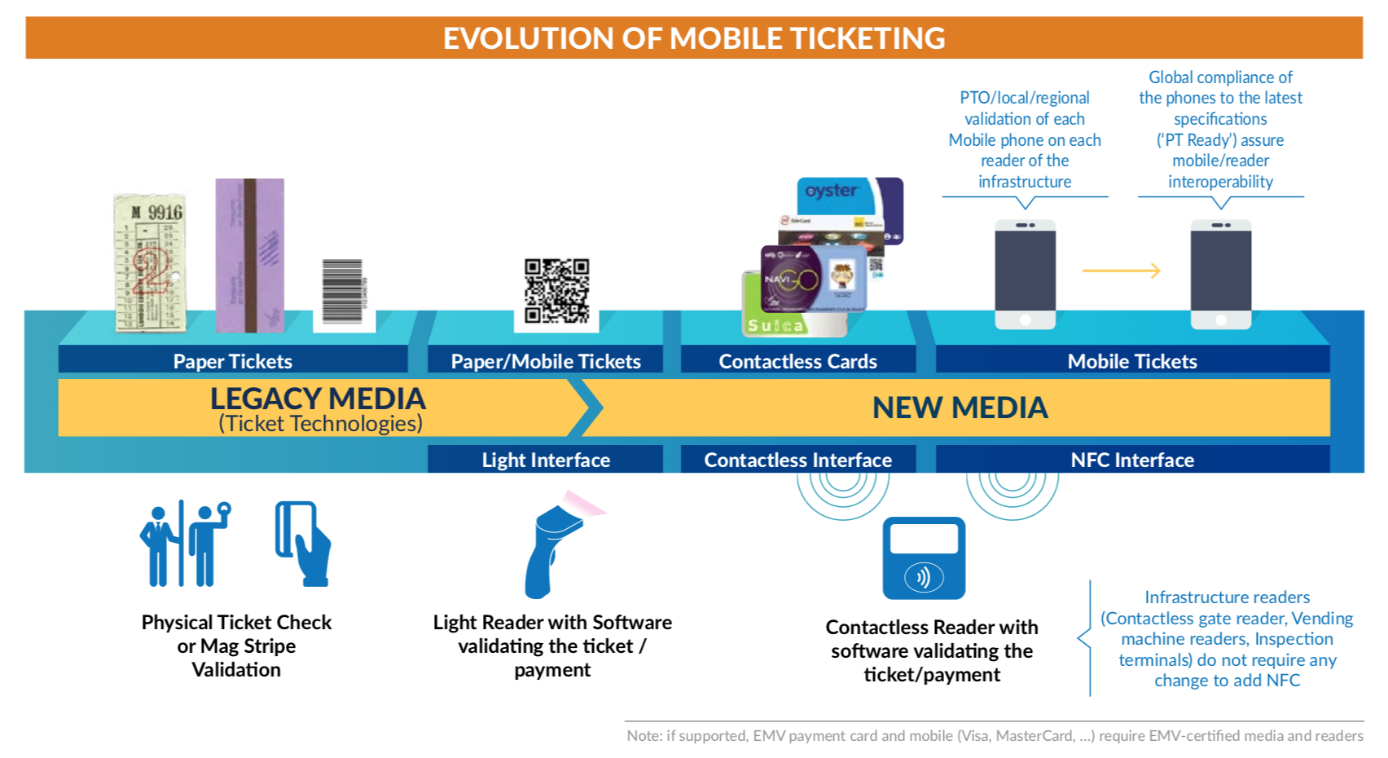
\includegraphics[width=0.9\linewidth]{image/smart_cards} \caption{The evolution of mobile ticketing (NFC Forum, 2016)}\label{fig:unnamed-chunk-6}
\end{figure}

Furthermore current research addresses the issues of big data and how collected data through contactless smart cards can be best analysed (see Kurauchi \& Schmöcker, 2017).

\hypertarget{current-state-of-art-in-practice-15}{%
\subsection*{Current state of art in practice}\label{current-state-of-art-in-practice-15}}
\addcontentsline{toc}{subsection}{Current state of art in practice}

Many countries, regions or cities, have smart card ticketing systems in use, like the whole of Netherlands, Helsinki Region, Minsk, Berlin, Auckland, Sydney and many more (see Wikipedia contributors, 2021). The systems itself differ and depend on the local ticketing and fare systems. While London, for instance, is using an access control system, Helsinki's system is trust based. Furthermore, a distinction can be made between pre-paid (debit) and post-paid (credit) systems (Kurauchi \& Schmöcker, 2017).

\hypertarget{relevant-initiatives-in-austria-16}{%
\subsection*{Relevant initiatives in Austria}\label{relevant-initiatives-in-austria-16}}
\addcontentsline{toc}{subsection}{Relevant initiatives in Austria}

\begin{itemize}
\tightlist
\item
  \href{https://taikai.network/en/wiener-linien/challenges/tickethon}{taikai.network}
\item
  \href{https://www.variuscard.com/}{variuscard}
\item
  \href{https://www.austriacard.com/}{austriacard}
\end{itemize}

\hypertarget{impacts-with-respect-to-sustainable-development-goals-sdgs-16}{%
\subsection*{Impacts with respect to Sustainable Development Goals (SDGs)}\label{impacts-with-respect-to-sustainable-development-goals-sdgs-16}}
\addcontentsline{toc}{subsection}{Impacts with respect to Sustainable Development Goals (SDGs)}

\begin{longtable}[]{@{}ccccc@{}}
\toprule
\begin{minipage}[b]{0.17\columnwidth}\centering
Impact level\strut
\end{minipage} & \begin{minipage}[b]{0.16\columnwidth}\centering
Indicator\strut
\end{minipage} & \begin{minipage}[b]{0.17\columnwidth}\centering
Impact direction\strut
\end{minipage} & \begin{minipage}[b]{0.17\columnwidth}\centering
Goal description and number\strut
\end{minipage} & \begin{minipage}[b]{0.17\columnwidth}\centering
Source\strut
\end{minipage}\tabularnewline
\midrule
\endhead
\begin{minipage}[t]{0.17\columnwidth}\centering
Individual\strut
\end{minipage} & \begin{minipage}[t]{0.16\columnwidth}\centering
Personal, travel expenditure reduced\strut
\end{minipage} & \begin{minipage}[t]{0.17\columnwidth}\centering
\textbf{+}\strut
\end{minipage} & \begin{minipage}[t]{0.17\columnwidth}\centering
Sustainable economic development (\emph{8,11})\strut
\end{minipage} & \begin{minipage}[t]{0.17\columnwidth}\centering
Turner \& Wilson, 2010\strut
\end{minipage}\tabularnewline
\begin{minipage}[t]{0.17\columnwidth}\centering
Individual\strut
\end{minipage} & \begin{minipage}[t]{0.16\columnwidth}\centering
Access to digitalised transport\strut
\end{minipage} & \begin{minipage}[t]{0.17\columnwidth}\centering
\textbf{+}\strut
\end{minipage} & \begin{minipage}[t]{0.17\columnwidth}\centering
Innovation \& Infrastructure (\emph{9})\strut
\end{minipage} & \begin{minipage}[t]{0.17\columnwidth}\centering
Turner \& Wilson, 2010\strut
\end{minipage}\tabularnewline
\begin{minipage}[t]{0.17\columnwidth}\centering
Systemic\strut
\end{minipage} & \begin{minipage}[t]{0.16\columnwidth}\centering
Public transport capacity increases\strut
\end{minipage} & \begin{minipage}[t]{0.17\columnwidth}\centering
\textbf{+}\strut
\end{minipage} & \begin{minipage}[t]{0.17\columnwidth}\centering
Sustainable economic development (\emph{8,11})\strut
\end{minipage} & \begin{minipage}[t]{0.17\columnwidth}\centering
Turner \& Wilson, 2010\strut
\end{minipage}\tabularnewline
\begin{minipage}[t]{0.17\columnwidth}\centering
Systemic\strut
\end{minipage} & \begin{minipage}[t]{0.16\columnwidth}\centering
Facilitates integration of the fare systems of several operators within a city\strut
\end{minipage} & \begin{minipage}[t]{0.17\columnwidth}\centering
\textbf{+}\strut
\end{minipage} & \begin{minipage}[t]{0.17\columnwidth}\centering
Partnership \& collaborations (\emph{17})\strut
\end{minipage} & \begin{minipage}[t]{0.17\columnwidth}\centering
Kurauchi \& Schmoecker, 2017\strut
\end{minipage}\tabularnewline
\bottomrule
\end{longtable}

\hypertarget{technology-and-societal-readiness-level-16}{%
\subsection*{Technology and societal readiness level}\label{technology-and-societal-readiness-level-16}}
\addcontentsline{toc}{subsection}{Technology and societal readiness level}

\begin{longtable}[]{@{}cc@{}}
\toprule
TRL & SRL\tabularnewline
\midrule
\endhead
7-9 & 7-9\tabularnewline
\bottomrule
\end{longtable}

\hypertarget{open-questions-16}{%
\subsection*{Open questions}\label{open-questions-16}}
\addcontentsline{toc}{subsection}{Open questions}

\begin{enumerate}
\def\labelenumi{\arabic{enumi}.}
\tightlist
\item
  How can the large amount of provided data be best used?
\item
  What advantages and disadvantages would an implementation in the main cities of Austria have?
\end{enumerate}

\hypertarget{further-links-14}{%
\subsection*{Further links}\label{further-links-14}}
\addcontentsline{toc}{subsection}{Further links}

\begin{itemize}
\tightlist
\item
  \href{https://www.itso.org.uk/}{itso}
\end{itemize}

\hypertarget{references-16}{%
\subsection*{References}\label{references-16}}
\addcontentsline{toc}{subsection}{References}

\begin{itemize}
\tightlist
\item
  Kurauchi, F., \& Schmöcker, J. D. (Eds.). (2017). Public transport planning with smart card data. CRC Press.
\item
  Mezghani, M. (2008). Study on electronic ticketing in public transport. European Metropolitan Transport Authorities (EMTA), 56, 38.
\item
  NFC Forum. (2016). NFC-enabled e-Ticketing in Public Transport\,: Clearing the Route to Interoperability. December. \url{https://nfc-forum.org/wp-content/uploads/2016/12/NFC_enabled_eTicketing_in_Public_Transport_White_Paper.pdf}
\item
  ÖBB. Ihr Weg zum Ticket. Retrieved 13th January 2021, from \url{https://www.oebb.at/de/tickets-kundenkarten/weg-zum-ticket}
\item
  Turner, M., \& Wilson, R. (2010). Smart and integrated ticketing in the UK: Piecing together the jigsaw. Computer Law \& Security Review, 26(2), 170-177.
\item
  Wels Linien. Tarife. Retrieved 13th January 2021, from \url{https://www.welslinien.at/tarife/}
\item
  Wiener Linien. (2021a). Der richtige Fahrschein,
  der passende Tarif. Retrieved 13th January 2021, from \url{https://www.wienerlinien.at/eportal3/ep/channelView.do/pageTypeId/66526/channelId/-46648}
\item
  Wiener Linien. (2021b). Digital-Wettbewerb ``Vienna Tickethon'' gestartet. Retrieved 13th January 2021, from \url{https://www.wienerlinien.at/eportal3/ep/contentView.do/pageTypeId/66526/programId/74577/contentTypeId/1001/channelId/-47186/contentId/5002360\#}:\textasciitilde:text=Im\%20Rahmen\%20eines\%20internationalen\%20Hackathon,Wettbewerb\%20l\%C3\%A4uft\%20bis\%20Anfang\%20M\%C3\%A4rz
\item
  Wikipedia contributors. (2021, January 8). List of smart cards. In Wikipedia, The Free Encyclopedia. Retrieved 15:30, January 13, 2021, from \url{https://en.wikipedia.org/w/index.php?title=List_of_smart_cards\&oldid=999040130}
\end{itemize}

\hypertarget{special_needs}{%
\section{Information and assistance for people with special needs}\label{special_needs}}

\hypertarget{synonyms-15}{%
\subsection*{Synonyms}\label{synonyms-15}}
\addcontentsline{toc}{subsection}{Synonyms}

\emph{Assistive technology}

\hypertarget{definition-17}{%
\subsection*{Definition}\label{definition-17}}
\addcontentsline{toc}{subsection}{Definition}

Vehmas (2010: 92) defines that having a special need \emph{``\ldots implies that an individual has the kind of characteristics that it is unlikely, or at least uncertain, whether he or she would achieve the aim that defines the need in question without special instruction, procedures that are out of ordinary.''} Special needs can therefore mean a mobility limitation due to age or any type of disability.

Furthermore, \emph{``Assistive technology refers to any system, services, appliances or devices that could be used to help disabled people with their daily life by removing some barriers to activities.''} (Low et al., 2020).

Because the types of disabilities are diverse and so are the specific needs, Low et al.~(2020) argue that more specific measures should be taken to meet the particular needs of specific disabilities rather than generalizing the types of assistive devices available. The requirements regarding traffic systems for people with special needs can be divided into \emph{(1)} visual impairment, \emph{(2)} hearing impairment, \emph{(3)} mobility impairment, and \emph{(4)} mental impairment. While for some people with special needs only one may be applicable, the elderly people might depend upon more than one or even all.

Low et al.~(2020) argue, that especially people with visual impairment (VIP) are dependent on public transport, because they cannot drive vehicles themselves, which leads to a restriction of freedom of movement. The same applies to many people with limited mobility who are excluded from active participation in motorized individual transport. Limited access to travel information is often a barrier to independent travel and other daily activities for people with special needs. When using public transportation, the choice of route is influenced by the reliability and availability of information, as well as convenience and comfort. However simply gathering this information before a trip can often be a problem for VIPs, as a lot of information is printed. However, the current trend towards online materials is helping. Due to physical and mental conditions, especially old or disabled people might need some extra information, for example, many older people cannot stand for long, are sensitive to weather conditions, cannot do things quickly or cannot walk long distances (Hounsell et al., 2016). A lack of usable information can add a negative aspect to the overall experience and actually prevent a trip.

In addition, Low et al.~(2020) argue, that bus riding poses several challenges for VIPs, such as finding the right bus, which is especially problematic when multiple bus stops are at the same station. The mix of fleets used makes it difficult for VIPs to identify the characteristics of a bus. Furthermore, it is often difficult for VIPs to locate the boarding point for buses. Regarding trains, the gap between the train and the platform can be a barrier. An important part of public transport are audio announcements, which serve as a source of information for VIPs. If these systems fail, the journey is perceived as particularly stressful.

To overcome barriers at the ticket buying, the implementation of contactless card systems (see \protect\hyperlink{contactless_cards}{Contactless public transport cards section}) or free passes for disabled people can help (Low et al., 2020).

\hypertarget{key-stakeholders-17}{%
\subsection*{Key stakeholders}\label{key-stakeholders-17}}
\addcontentsline{toc}{subsection}{Key stakeholders}

\begin{itemize}
\tightlist
\item
  \textbf{Affected}: People with special needs, elderly population, care takers
\item
  \textbf{Responsible}: Transport service providers and public transport operators, MaaS operators and integrators, IT system providers, city councils, local, regional and national authorities, public transport associations, industry suppliers, Association for the Blind, Association for the Disabled
\end{itemize}

\hypertarget{current-state-of-art-in-research-17}{%
\subsection*{Current state of art in research}\label{current-state-of-art-in-research-17}}
\addcontentsline{toc}{subsection}{Current state of art in research}

The study by Low et al.~(2020) reflects, among other things, VIPs' desire to be independent in planning their trips by using online resources rather than seeking help from others. This shows the importance of having appropriate online tools for VIPs. Interviewees mentioned that they need to use many different sources and apps to plan a single trip, which in turn causes a lot of stress and decreases the propensity to the use of public transport. In addition, VIPs were found to lack access to current policies and information on available assistance. Furthermore, it was pointed out, that a similar interior design of buses would be extremely helpful for VIP and increase safety.

Goldberg et al.~(2018) looked into the needs of VIPs for orientation, navigation and mobility. Based on their findings, they propose \emph{``an integrated cyber-physical system (CPS) framework with `Agents' and `Smart Environments' to address VIP's ONM needs in urban settings.''} Fusco \& Coughlan (2020) described \emph{``a computer vision approach to indoor localization that runs as a real-time app on a conventional smart-phone, which is intended to support a full-featured wayfinding app in the future that will include turn-by-turn directions.''} One advantage of this approach is that no new infrastructure is needed, just a working smartphone with a built-in camera.

Hounsell et al.~(2016) addressed information needs of older people particularly using public transport. Among other things, they found that elderly people \emph{``may need larger font displays and primary data only, while mobility impaired people may need information on walking distances and the existence of gradient, steps, seats, etc.''} By reviewing international cases of open data implementation, they found examples of authorities initiating the market by running competitions to develop apps for targeted groups such as older or disabled people.

\hypertarget{current-state-of-art-in-practice-16}{%
\subsection*{Current state of art in practice}\label{current-state-of-art-in-practice-16}}
\addcontentsline{toc}{subsection}{Current state of art in practice}

One of the common assistive tools available to VIP are mobility tools, in particular a long cane or a guide dog. GPS is used as an assistive technology for VIP for orientation purposes and as a navigation aid. It can also be integrated into other devices to help VIP with orientation, such as a GPS-based voice alarm system that alerts VIP to nearby obstacles (Low et al., 2020). \emph{BlindSquare} is one of the most popular GPS apps in the world for blind and visually impaired people. It describes the surroundings, warns about street intersections and important points as one moves along. Used in conjunction with external free navigation apps, \emph{BlindSquare} provides almost all the information blind and visually impaired people need to be independent on the road. \emph{BlindSquare} determines the location using the smartphone's GPS capabilities and retrieves information about the surrounding area on Foursquare and Open Street Map. Thanks to its unique algorithms, it determines the most relevant information and states it clearly in an artificial voice (BlindSquare., n.d.). A similar app is \emph{Seeing Assistant Move}, which is based on Google Maps and also works offline and with voice control (Transition Technologies S.A., n.d.). Using public transport audio announcements plays a crucial role in helping VIP to be prepared to alight from the vehicle (Low et al., 2020).

Induction hearing systems or induction hearing loops are used to provide people with hearing problems with auditory information. The principle is based on special cables, the so-called induction loop, which is operated by an induction amplifier that converts the signals coming from the microphone and feeds them into the loop as a current. This current, in turn, creates a weak magnetic field in the coil in the room, which pulses in rhythm with the speech. This weak magnetic field is picked up by the hearing aid's T-coil, similar to an antenna, and converted back into audible sound vibrations. Almost no background noise is transmitted and the desired information can thus be heard without interference, almost in HIFI quality (Sturma, 2011).

To ensure accessibility for people with limited mobility in buses, more and more cities are focusing on the use of low-floor vehicles that can be lowered further hydraulically if required. The low entrance height makes boarding and alighting much easier, especially for older people and passengers with baby carriages or wheelchair users. Tramway equipment is also constantly being improved. Modern cars have more space for passengers with wheelchairs or baby carriages and a retractable ramp to bridge the already minimized gap between the platform edge and the vehicle (Wiener Linien, n.d.). As in Vienna, for example, real-time displays at stations can use a wheelchair symbol to indicate whether the expected public transport vehicles are barrier-free.

Finally, for example in Singaporean buses were introduced amenities for the convenience of pregnant, elderly and young passengers in the form of designated priority seats, low floors along the entire bus and low steps at the entrance and exit to facilitate individuals with limited mobility to board the bus quickly as well as move along the bus more easily (Smrt.com.sg, 2021).

\hypertarget{relevant-initiatives-in-austria-17}{%
\subsection*{Relevant initiatives in Austria}\label{relevant-initiatives-in-austria-17}}
\addcontentsline{toc}{subsection}{Relevant initiatives in Austria}

\begin{itemize}
\tightlist
\item
  \href{https://www.oebb.at/de/reiseplanung-services/barrierefrei-reisen}{oebb.at}
\item
  \href{https://www.wienerlinien.at/web/wiener-linien/neue-bim-und-bus-haltestellen-f\%C3\%BCr-wien}{wienerlinien.at}
\item
  \href{https://www.induktionsschleife.at/}{induktionsschleife.at}
\end{itemize}

\hypertarget{impacts-with-respect-to-sustainable-development-goals-sdgs-17}{%
\subsection*{Impacts with respect to Sustainable Development Goals (SDGs)}\label{impacts-with-respect-to-sustainable-development-goals-sdgs-17}}
\addcontentsline{toc}{subsection}{Impacts with respect to Sustainable Development Goals (SDGs)}

\begin{longtable}[]{@{}ccccc@{}}
\toprule
\begin{minipage}[b]{0.17\columnwidth}\centering
Impact level\strut
\end{minipage} & \begin{minipage}[b]{0.16\columnwidth}\centering
Indicator\strut
\end{minipage} & \begin{minipage}[b]{0.17\columnwidth}\centering
Impact direction\strut
\end{minipage} & \begin{minipage}[b]{0.17\columnwidth}\centering
Goal description and number\strut
\end{minipage} & \begin{minipage}[b]{0.17\columnwidth}\centering
Source\strut
\end{minipage}\tabularnewline
\midrule
\endhead
\begin{minipage}[t]{0.17\columnwidth}\centering
Individual\strut
\end{minipage} & \begin{minipage}[t]{0.16\columnwidth}\centering
Safe access to public transport\strut
\end{minipage} & \begin{minipage}[t]{0.17\columnwidth}\centering
\textbf{+}\strut
\end{minipage} & \begin{minipage}[t]{0.17\columnwidth}\centering
Health \& Wellbeing (\emph{3})\strut
\end{minipage} & \begin{minipage}[t]{0.17\columnwidth}\centering
Low et al.~(2020)\strut
\end{minipage}\tabularnewline
\begin{minipage}[t]{0.17\columnwidth}\centering
Individual\strut
\end{minipage} & \begin{minipage}[t]{0.16\columnwidth}\centering
Equal freedom of movement\strut
\end{minipage} & \begin{minipage}[t]{0.17\columnwidth}\centering
\textbf{+}\strut
\end{minipage} & \begin{minipage}[t]{0.17\columnwidth}\centering
Equality (\emph{5,10})\strut
\end{minipage} & \begin{minipage}[t]{0.17\columnwidth}\centering
Low et al.~(2020)\strut
\end{minipage}\tabularnewline
\begin{minipage}[t]{0.17\columnwidth}\centering
Individual\strut
\end{minipage} & \begin{minipage}[t]{0.16\columnwidth}\centering
Improved access to public transport\strut
\end{minipage} & \begin{minipage}[t]{0.17\columnwidth}\centering
\textbf{+}\strut
\end{minipage} & \begin{minipage}[t]{0.17\columnwidth}\centering
Environmental sustainability (\emph{7,12-13,15})\strut
\end{minipage} & \begin{minipage}[t]{0.17\columnwidth}\centering
Low et al.~(2020)\strut
\end{minipage}\tabularnewline
\begin{minipage}[t]{0.17\columnwidth}\centering
Systemic\strut
\end{minipage} & \begin{minipage}[t]{0.16\columnwidth}\centering
Increase in innovative apps developed for targeted groups; use of open data\strut
\end{minipage} & \begin{minipage}[t]{0.17\columnwidth}\centering
\textbf{+}\strut
\end{minipage} & \begin{minipage}[t]{0.17\columnwidth}\centering
Innovation \& Infrastructure (\emph{9})\strut
\end{minipage} & \begin{minipage}[t]{0.17\columnwidth}\centering
Hounsell et al.~(2016)\strut
\end{minipage}\tabularnewline
\bottomrule
\end{longtable}

\hypertarget{technology-and-societal-readiness-level-17}{%
\subsection*{Technology and societal readiness level}\label{technology-and-societal-readiness-level-17}}
\addcontentsline{toc}{subsection}{Technology and societal readiness level}

\begin{longtable}[]{@{}cc@{}}
\toprule
TRL & SRL\tabularnewline
\midrule
\endhead
3-7 & 3-7\tabularnewline
\bottomrule
\end{longtable}

\hypertarget{open-questions-17}{%
\subsection*{Open questions}\label{open-questions-17}}
\addcontentsline{toc}{subsection}{Open questions}

\begin{enumerate}
\def\labelenumi{\arabic{enumi}.}
\tightlist
\item
  How could real-time information be better available for visually impaired people?
\item
  How could audio announcements be improved?
\item
  How to improve staff assistance?
\item
  How could smart technologies become more accessible to older people?
\end{enumerate}

\hypertarget{further-links-15}{%
\subsection*{Further links}\label{further-links-15}}
\addcontentsline{toc}{subsection}{Further links}

\begin{itemize}
\tightlist
\item
  \href{https://www.blindsquare.com/de/about/}{blindsquare.com}
\item
  \href{http://seeingassistant.tt.com.pl/move/}{seeingassistant.tt.com.pl}
\item
  \href{https://www.induktionsschleife.at/anwendungen/}{induktionsschleife.at}
\item
  \href{https://www.oebb.at/de/reiseplanung-services/barrierefrei-reisen}{oebb.at}
\item
  \href{https://www.wienerlinien.at/eportal3/ep/contentView.do?pageTypeId=66526\&channelId=-47186\&programId=74577\&contentId=5002349\&contentTypeId=1001}{wienerlinien.at}
\item
  \href{https://www.oesb-dachverband.at/}{oesb-dachverband.at}
\item
  \href{https://www.blindenverband.at/}{blindenverband.at}
\end{itemize}

\hypertarget{references-17}{%
\subsection*{References}\label{references-17}}
\addcontentsline{toc}{subsection}{References}

\begin{itemize}
\tightlist
\item
  BlindSquare. (n.d.). What is BlindSquare? Retrieved March 4, 2021, from \url{https://www.blindsquare.com/about/}
\item
  Fusco, G., \& Coughlan, J. M. (2020, April). Indoor localization for visually impaired travelers using computer vision on a smartphone. In Proceedings of the 17th International Web for All Conference (pp.~1-11).
\item
  Goldberg, M., Zhu, Z., \& Zhang, Z. (2018). How do we aid visually impaired people safely manage unfamiliar environments?.
\item
  Hounsell, N. B., Shrestha, B. P., McDonald, M., \& Wong, A. (2016). Open data and the needs of older people for public transport information. Transportation research procedia, 14, 4334-4343.
\item
  Low, W. Y., Cao, M., De Vos, J., \& Hickman, R. (2020). The journey experience of visually impaired people on public transport in London. Transport Policy, 97, 137-148.
\item
  Smrt.com.sg. (2021). Accessibility. {[}online{]} Smrt.com.sg. Available at: \url{https://www.smrt.com.sg/Journey-with-Us/SMRT-Buses/Accessibility} {[}Accessed 12 March 2021{]}.
\item
  Sturma, A. (2011). Höranlagen. \url{https://www.oessh.or.at/hoerspuren/hoeranlagen}
\item
  Transition Technologies S.A. (n.d.). Seeing Assistant Move - Features. Retrieved March 4, 2021, from \url{http://seeingassistant.tt.com.pl/move/}
\item
  Vehmas, S. (2010). Special needs: a philosophical analysis. International journal of inclusive education, 14(1), 87-96.
\item
  Wiener Linien. (n.d.). Barrierefreiheit bei den Wiener Linien - Wiener Linien. Retrieved March 16, 2021, from \url{https://www.wienerlinien.at/web/wiener-linien/barrierefreiheit}
\end{itemize}

\hypertarget{mobility_hubs}{%
\section{Mobility hubs}\label{mobility_hubs}}

\hypertarget{connected}{%
\chapter{Autonomous driving}\label{connected}}

\hypertarget{av}{%
\section{Automated vehicles}\label{av}}

\hypertarget{parking_av}{%
\section{Parking infrastructure for autonomous vehicles}\label{parking_av}}

\hypertarget{onboard}{%
\chapter{On-board technology for connected and automated vehicles}\label{onboard}}

\hypertarget{adas}{%
\section{Advanced driver assistance system (ADAS)}\label{adas}}

\hypertarget{parking_assistance}{%
\section{Parking assistance system}\label{parking_assistance}}

\hypertarget{definition-18}{%
\subsection*{Definition}\label{definition-18}}
\addcontentsline{toc}{subsection}{Definition}

Nowadays, parking a car becomes an increasingly mundane task due to the growing size of the vehicles which consequently reduces visibility to the rear and front. Moreover, the number of vehicles on the road continues to increase which makes finding parking spaces more difficult. To overcome this challenge, efficient and advanced parking techniques are needed, such as finding the right parking space and parking cars efficiently (Khalid et al., 2021).
While in the 1990s parking assistance systems were not considered necessary, systems that support the parking process are now standard in new vehicles and have a high acceptance rate. While parking assistance systems of the first generations were mainly informative systems, today these systems help to find a suitable parking space and support the steering during the parking manoeuvre. Future systems will become even more autonomous, up to a point where they will find their parking space without human intervention (Valet Parking) (Gotzig, 2016).
With respect to safety issues, parking assistance systems can reduce insurance claims that occur during parking manoeuvres by 30\% (ADAC, 2020). They also provide a useful application in the form of emergency brake assistant that prevents accidents with other road users when reversing (ADAC, 2019).
Modern Parking assistants work with two sensor concepts: ultrasonic sensors for the close range at the rear (often already installed as ``parking beepers'') and radar sensors with a longer range at the side in the bumper (ADAC, 2019). Additionally, there are also new releases with 360° view around the car (Land Rover, no date; Mercedes-Benz, no date). However, there are no tests for this at the moment.

\hypertarget{key-stakeholders-18}{%
\subsection*{Key stakeholders}\label{key-stakeholders-18}}
\addcontentsline{toc}{subsection}{Key stakeholders}

\begin{itemize}
\tightlist
\item
  \textbf{Affected}: Car Drivers, Traffic participants, Insurers
\item
  \textbf{Responsible}: Car manufacturers
\end{itemize}

\hypertarget{current-state-of-art-in-research-18}{%
\subsection*{Current state of art in research}\label{current-state-of-art-in-research-18}}
\addcontentsline{toc}{subsection}{Current state of art in research}

The research on on-board parking features is almost entirely owned by the car manufacturers. Research tends to focus on larger-scale issues such as car parking location tracking, space booking systems using IoT and congestion caused by \emph{parking cruises}.
Additionally, tests are carried out on the merger between emergency brake assistant and parking assistant to overcome the difficulties with obstacles detection and reduce the collision rates in this specific situation. The ADAC tested the AEB (Autonomous Emergency Braking) systems from Mercedes, Volvo, BMW, Seat and Skoda in three test scenarios: \emph{(1)} a pedestrian dummy stands behind a car or walks past, \emph{(2)} a car parks in the direction of travel and \emph{(3)} cyclists as well as cars drive past crosswise.
BMW was the best at reacting to all situations with radar and ultrasound - with some drop-outs, especially with moving pedestrians or cross-traffic. The Mercedes, on the other hand, only used its side radar sensors for reverse braking and thus did not recognise stationary vehicles at all. The VW system from Skoda and Seat had radar and ultrasound, but moving pedestrians were only detected randomly or not at all.
Overall, these tests showed that the automatic braking parking assistants have a lot of potential, but are far from optimal. Even the system of the front-runner does not yet work 100\% reliably. Even the low-cost ultrasonic sensors, however, can be very effective and even prevent pedestrian collisions, as the BMW showed in the test. Therefore, it is crucial that manufacturers equip their vehicles with an effective AEB system as a standard. The necessary technology is already available in most passenger cars where the rear ultrasonic sensors would need to be linked to the braking function (ADAC, 2019).
The greatest difficulties are encountered in pedestrian detection, in the scenarios in which the risk of personal injury is potentially the highest. Some of the tested vehicles recognised the dangerous situation too late or not at all.

\hypertarget{current-state-of-art-in-practice-17}{%
\subsection*{Current state of art in practice}\label{current-state-of-art-in-practice-17}}
\addcontentsline{toc}{subsection}{Current state of art in practice}

Nearly 50\% of the cars in Germany are now equipped with parking assistance. Nonetheless, the results of a study by HUK-Coburg, Germany's largest motor insurer with eleven million insured cars, show that the number of fender-benders has not decreased and the damage costs have even risen slightly. The reason for this is the damage to the expensive Park Distance Control (PDC) sensor embedded in the bumper when vehicle collides with an obstacle while parking (Focus Online, 2017).
In 2017, 570 accidents with personal injury occurred in Austria when reversing with passenger cars. There were no fatalities, but around 290 people were injured, 60 of them seriously. In addition, there is a large amount of property damage due to obstacles being overlooked (ÖAMTC, 2019).
According to different sources, between 23\% and 46\% of the cars in Germany are equipped with an on-board parking assistant (Focus Online, 2017). In contrast, only 13\% of the vehicles are equipped with an emergency brake assistant that automatically brakes in the event of an imminent collision with the vehicle in front or even detects pedestrians and cyclists. Further, a survey conducted on 1000 respondents by German Road Safety Council showed that 85\% of the sample found the emergency brake assistant as highly useful and 65\% considered parking assistant highly beneficial (Handelsblatt, 2016).
Currently, the most advanced technology with respect to parking assistance is offered by Tesla S, where the system is fully autonomous and allows the car to drive itself out of a tight space without the driver's intervention. But it is expected that the technology will be available from other manufacturers too and will improve rapidly in the coming years. One reason for this is that parking assistants with brake intervention will become part of the European vehicle test programme \emph{Euro NCAP} from 2020. In the past, it has been shown that the inclusion of active and passive passenger car safety systems in this programme quickly increases the rate at which vehicles are equipped (ÖAMTC, 2019).

\hypertarget{relevant-initiatives-in-austria-18}{%
\subsection*{Relevant initiatives in Austria}\label{relevant-initiatives-in-austria-18}}
\addcontentsline{toc}{subsection}{Relevant initiatives in Austria}

\begin{itemize}
\tightlist
\item
  \href{https://www.oeamtc.at/tests/assistenzsystemtest/fuenf-parkassistenten-mit-notbremssystem-im-test-31717317}{oeamtc.at}
\end{itemize}

\hypertarget{impacts-with-respect-to-sustainable-development-goals-sdgs-18}{%
\subsection*{Impacts with respect to Sustainable Development Goals (SDGs)}\label{impacts-with-respect-to-sustainable-development-goals-sdgs-18}}
\addcontentsline{toc}{subsection}{Impacts with respect to Sustainable Development Goals (SDGs)}

\begin{longtable}[]{@{}ccccc@{}}
\toprule
\begin{minipage}[b]{0.17\columnwidth}\centering
Impact level\strut
\end{minipage} & \begin{minipage}[b]{0.16\columnwidth}\centering
Indicator\strut
\end{minipage} & \begin{minipage}[b]{0.17\columnwidth}\centering
Impact direction\strut
\end{minipage} & \begin{minipage}[b]{0.17\columnwidth}\centering
Goal description and number\strut
\end{minipage} & \begin{minipage}[b]{0.17\columnwidth}\centering
Source\strut
\end{minipage}\tabularnewline
\midrule
\endhead
\begin{minipage}[t]{0.17\columnwidth}\centering
Individual\strut
\end{minipage} & \begin{minipage}[t]{0.16\columnwidth}\centering
Road accidents when parking reduced\strut
\end{minipage} & \begin{minipage}[t]{0.17\columnwidth}\centering
\textbf{+}\strut
\end{minipage} & \begin{minipage}[t]{0.17\columnwidth}\centering
Health \& Wellbeing (\emph{3})\strut
\end{minipage} & \begin{minipage}[t]{0.17\columnwidth}\centering
ADAC, 2019\strut
\end{minipage}\tabularnewline
\begin{minipage}[t]{0.17\columnwidth}\centering
Individual\strut
\end{minipage} & \begin{minipage}[t]{0.16\columnwidth}\centering
Higher costs in case of collision\strut
\end{minipage} & \begin{minipage}[t]{0.17\columnwidth}\centering
\textbf{-}\strut
\end{minipage} & \begin{minipage}[t]{0.17\columnwidth}\centering
Sustainable economic development (\emph{8,11})\strut
\end{minipage} & \begin{minipage}[t]{0.17\columnwidth}\centering
Focus Online, 2017\strut
\end{minipage}\tabularnewline
\begin{minipage}[t]{0.17\columnwidth}\centering
Systemic\strut
\end{minipage} & \begin{minipage}[t]{0.16\columnwidth}\centering
New designs tested\strut
\end{minipage} & \begin{minipage}[t]{0.17\columnwidth}\centering
\textbf{+}\strut
\end{minipage} & \begin{minipage}[t]{0.17\columnwidth}\centering
Innovation \& Infrastructure (\emph{9})\strut
\end{minipage} & \begin{minipage}[t]{0.17\columnwidth}\centering
Euro NCAP, 2021\strut
\end{minipage}\tabularnewline
\bottomrule
\end{longtable}

\hypertarget{technology-and-societal-readiness-level-18}{%
\subsection*{Technology and societal readiness level}\label{technology-and-societal-readiness-level-18}}
\addcontentsline{toc}{subsection}{Technology and societal readiness level}

\begin{longtable}[]{@{}cc@{}}
\toprule
TRL & SRL\tabularnewline
\midrule
\endhead
8-9 & 8-9\tabularnewline
\bottomrule
\end{longtable}

\hypertarget{open-questions-18}{%
\subsection*{Open questions}\label{open-questions-18}}
\addcontentsline{toc}{subsection}{Open questions}

\begin{enumerate}
\def\labelenumi{\arabic{enumi}.}
\tightlist
\item
  How can acceptance and usability rates be increased in drivers especially in elderly group?
\item
  What are the legal implications for the use of assisted parking for both drivers and car manufacturers?
\end{enumerate}

\hypertarget{references-18}{%
\subsection*{References}\label{references-18}}
\addcontentsline{toc}{subsection}{References}

\begin{itemize}
\tightlist
\item
  ADAC. (2019, May 14). Parkassistenten im Test: Noch nicht gut genug. \url{https://presse.adac.de/meldungen/adac-ev/tests/parkassistent.html}
\item
  ADAC. (2020, January 9). Fahrerassistenzsysteme im Überblick \textbar{} ADAC. \url{https://www.adac.de/rund-ums-fahrzeug/ausstattung-technik-zubehoer/assistenzsysteme/fahrerassistenzsysteme/}
\item
  Euro NCAP. (2021). \url{http://www.euroncap.com} (Accessed: 26 February 2021)
\item
  Focus Online. (2017, April 27). Einparkhilfen bringen nichts - sondern verursachen mehr Schaden - FOCUS Online. \url{https://www.focus.de/auto/news/untersuchung-der-huk-coburg-studie-einparkhilfe-hilft-nicht-sie-versucht-eher-mehr-schaden_id_7035248.html}
\item
  Gotzig, H. (2016). Parking Assistance. In H. Winner, S. Hakuli, F. Lotz, \& C. Singer (Eds.), Handbook of Driver Assistance Systems: Basic Information, Components and Systems for Active Safety and Comfort (pp.~1077--1092). Springer International Publishing. \url{https://doi.org/10.1007/978-3-319-12352-3_45}
\item
  Handelsblatt. (2016, April 8). Umfrage zu Assistenzsystemen\,: Einparkassistent nützlich, Notbremsassistent nützlicher. \url{https://www.handelsblatt.com/auto/nachrichten/umfrage-zu-assistenzsystemen-einparkassistent-nuetzlich-notbremsassistent-nuetzlicher/13404708.html?ticket=ST-4955434-naHBLAxI66h66nbvrBXF-ap1}
\item
  Khalid, M., Wang, K., Aslam, N., Cao, Y., Ahmad, N., \& Khan, M. K. (2021). From smart parking towards autonomous valet parking: A survey, challenges and future Works. Journal of Network and Computer Applications, 175, 102935. \url{https://doi.org/https://doi.org/10.1016/j.jnca.2020.102935}
\item
  Land Rover. (n.d.). Parking Assistance \textbar{} InControl \textbar{} Land Rover UK. Retrieved 25 February 2021, from \url{https://www.landrover.co.uk/incontrol/driver-safety-and-assistance/parking-assistance.html}
\item
  Margreiter, M., Mayer, P., Alpas, M., \& Vlahogianni, E. (2017). Driver's Willingness to Use Parking Assistance Tools and their Expectations: A Case Study for the Cities of Munich and Athens. In 8th International Congress on Transportation Research.
\item
  Mercedes-Benz. (n.d.). Mercedes-Benz X-Klasse: Park-Paket mit 360°-Kamera. Retrieved 25 February 2021, from \url{https://www.mercedes-benz.at/passengercars/mercedes-benz-cars/models/x-class/x-class-pickup/facts-and-lines/equipment-packages/360-camera.html}
\item
  Tsugawa, S. (2006). Trends and issues in safe driver assistance systems: Driver acceptance and assistance for elderly drivers. IATSS research, 30(2), 6-18.
\item
  ÖAMTC. (2019, May 14). ÖAMTC: Fünf Parkassistenten mit Notbremssystem im Test (+ Fotos, + Grafik) \textbar{} ÖAMTC, 14.05.2019. \url{https://www.ots.at/presseaussendung/OTS_20190514_OTS0021/oeamtc-fuenf-parkassistenten-mit-notbremssystem-im-test-fotos-grafik}
\end{itemize}

\hypertarget{lane_keeping}{%
\section{Lane keeping}\label{lane_keeping}}

\hypertarget{synonyms-16}{%
\subsection*{Synonyms}\label{synonyms-16}}
\addcontentsline{toc}{subsection}{Synonyms}

\emph{Lane Keeping Assist System (LKAS), Lane Keeping Assist (LKA)}

\hypertarget{definition-19}{%
\subsection*{Definition}\label{definition-19}}
\addcontentsline{toc}{subsection}{Definition}

Lane keeping assist monitors road markings, typically using a camera located behind the windscreen to keep the car within its driving lane and as a result reduce the burden of the driver. There are different systems currently available and they are not the same (Autonationdrive, 2019):

\begin{itemize}
\tightlist
\item
  \textbf{Lane Departure Warning (LDW)}: Audible or visual warnings signal to the driver that their vehicle is approaching or may be crossing the lane markings.
\item
  \textbf{Road Departure Assist (RDA)}: An automatic steering system, which may also include an automatic braking system, keeps the vehicle on the roadway itself.
\item
  \textbf{Lane Keeping Assist (LKA)}: An automatic steering system, which may also include an automatic braking system, keeps the vehicle within its lane.
\item
  \textbf{Lane Centering Assist (LCA)}: An automatic steering system, which may also include an automatic braking system, to keep the vehicle in the center of the lane.
\end{itemize}

The main difference betwenn them is that LDW informs the driver in case of crossing the road marking through different sensory cues such as tactile, visual or audio, the LKAS helps the driver to stay within the lane through the adjustments to steering wheel movements depending on the distance from the lane marking on either side. The systems can use reactive or proactive process, where the vehicle is reactively put back on track while it begins to leave the lane or proactively kept in the centre of the lane, respectively. It is usually activated by the driver and works at speed between 65 km/h and 180 km/h and radius of 230 m. Hence, it is the most suitable for highways and motorways but less so for urban or country roads. Even though the LKAS is activated, the driver remains responsible for controlling the vehicle. Consequently, LKAS continuously checks the steering movements applied by the driver and if he has his/her hands on the steering wheel. In case, the system detects that driver is not actively steering, it produces the waring and deactivates. This is to ensure that the driver remains in control throughout. Moreover, the driver can overrule the LKAS at any time. For example, LKAS deactivates automatically when braking and deliberate lane charge activated via the use of indicators (blinkers) (VDA, 2021).

\hypertarget{key-stakeholders-19}{%
\subsection*{Key stakeholders}\label{key-stakeholders-19}}
\addcontentsline{toc}{subsection}{Key stakeholders}

\begin{itemize}
\tightlist
\item
  \textbf{Affected}: General public, Drivers, Road infrastructure companies, Insurers
\item
  \textbf{Responsible}: Car manufacturers, Transport agencies, National governments and International bodies (eg. EU or \href{https://unece.org/fileadmin/DAM/trans/main/wp29/wp29regs/2018/R079r4e.pdf}{UNECE})
\end{itemize}

\hypertarget{current-state-of-art-in-research-19}{%
\subsection*{Current state of art in research}\label{current-state-of-art-in-research-19}}
\addcontentsline{toc}{subsection}{Current state of art in research}

Current research explores new approaches to the development of lane keeping assistance such as the use of Global Navigation Satellite System (Tominaga et al., 2020), deep learning (Wang et al., 2020) or neural network techniques (Yusuf et al., 2020). Beyond, it aims at the validation and improvement of LKAS by looking at the impact of system design (Lee et al., 2018) and different road conditions on the overall quality performance of lane keeping assistance (Romano et al., 2020). Further, a number of studies explored the potential of including driver's characteristics to develop of personalised lane keeping assist.
Further, study by Weaver \& Gonzalez (2020) focused on the influence of LKAS on drivers' behaviour and acceptance level of LKAS technology. It not only confirmed existing findings that more experience and familiarity with the system increases acceptance rate and trust, but it also showed a positive response from individuals who had no previous experience in using LKAS.

\hypertarget{current-state-of-art-in-practice-18}{%
\subsection*{Current state of art in practice}\label{current-state-of-art-in-practice-18}}
\addcontentsline{toc}{subsection}{Current state of art in practice}

In Europe the main existing legal basis for lane keeping systems that regulate its use is \href{https://op.europa.eu/en/publication-detail/-/publication/bfd5eba8-2058-11ea-95ab-01aa75ed71a1/language-en}{Regulation (EU) 2019/2144}. Hence, many car manufacturers nowadays offer cars featured with lane keeping assist which together with other system such as automatic cruise control or \protect\hyperlink{distance_keeping}{distance keeping} already provide a high level of automation. Some of many producers offering LKAS are \href{https://www.bosch-mobility-solutions.com/en/products-and-services/passenger-cars-and-light-commercial-vehicles/driver-assistance-systems/lane-keeping-assist/}{BOSCH}, \href{https://www.hondainfocenter.com/2021/CR-V/Feature-Guide/Interior-Features/Lane-Keeping-Assist-System-LKAS/}{Honda}, \href{https://www.tesla.com/de_DE/blog/more-advanced-safety-tesla-owners?redirect=no}{Tesla} or \href{https://owner.ford.com/support/how-tos/safety/driver-assist-technology/driving/how-to-use-lane-keeping-system.html}{Ford}.

In terms of the accident prevention, lane keeping assist has a huge potential to increase road safety where National Highway Traffic Safety Administration (NHTSA) data from 2011 show that 53\% of road fatalities result from a roadway departure (Automotive World, 2013). In fact, real world data from Sweden shows that crashes involving out-of-lane drift were reduced by 40\% for cars with Electonic Stability Control (ESC) as opposed to 29\% for cars without it (Sternlung, 2018).

The major disadvantage of lane keeping systems is the fact that it relies on a visual detection of painted road marking in order to work effectively therefore any condition deterioration such as nighttime or rain have a significant impact on the system performance (Tchir, 2019).

\hypertarget{relevant-initiatives-in-austria-19}{%
\subsection*{Relevant initiatives in Austria}\label{relevant-initiatives-in-austria-19}}
\addcontentsline{toc}{subsection}{Relevant initiatives in Austria}

\begin{itemize}
\tightlist
\item
  \href{https://www.ertrac.org/uploads/images/ERTRAC2019-Connected-Automated-Driving-Roadmap\%20-2019-04-04.pdf}{ertrac.org}
\end{itemize}

\hypertarget{impacts-with-respect-to-sustainable-development-goals-sdgs-19}{%
\subsection*{Impacts with respect to Sustainable Development Goals (SDGs)}\label{impacts-with-respect-to-sustainable-development-goals-sdgs-19}}
\addcontentsline{toc}{subsection}{Impacts with respect to Sustainable Development Goals (SDGs)}

\begin{longtable}[]{@{}ccccc@{}}
\toprule
\begin{minipage}[b]{0.17\columnwidth}\centering
Impact level\strut
\end{minipage} & \begin{minipage}[b]{0.16\columnwidth}\centering
Indicator\strut
\end{minipage} & \begin{minipage}[b]{0.17\columnwidth}\centering
Impact direction\strut
\end{minipage} & \begin{minipage}[b]{0.17\columnwidth}\centering
Goal description and number\strut
\end{minipage} & \begin{minipage}[b]{0.17\columnwidth}\centering
Source\strut
\end{minipage}\tabularnewline
\midrule
\endhead
\begin{minipage}[t]{0.17\columnwidth}\centering
Individual\strut
\end{minipage} & \begin{minipage}[t]{0.16\columnwidth}\centering
Accident risk reduced; low performance in suboptimal road conditions\strut
\end{minipage} & \begin{minipage}[t]{0.17\columnwidth}\centering
\textbf{\textasciitilde{}}\strut
\end{minipage} & \begin{minipage}[t]{0.17\columnwidth}\centering
Health \& Wellbeing (\emph{3})\strut
\end{minipage} & \begin{minipage}[t]{0.17\columnwidth}\centering
Sterlund, 2018; Tchir, 2019\strut
\end{minipage}\tabularnewline
\begin{minipage}[t]{0.17\columnwidth}\centering
Systemic\strut
\end{minipage} & \begin{minipage}[t]{0.16\columnwidth}\centering
Systems are continuously improved\strut
\end{minipage} & \begin{minipage}[t]{0.17\columnwidth}\centering
\textbf{+}\strut
\end{minipage} & \begin{minipage}[t]{0.17\columnwidth}\centering
Innovation \& Infrastructure (\emph{9})\strut
\end{minipage} & \begin{minipage}[t]{0.17\columnwidth}\centering
Lawrence \& Kareta, 2020\strut
\end{minipage}\tabularnewline
\bottomrule
\end{longtable}

\hypertarget{technology-and-societal-readiness-level-19}{%
\subsection*{Technology and societal readiness level}\label{technology-and-societal-readiness-level-19}}
\addcontentsline{toc}{subsection}{Technology and societal readiness level}

\begin{longtable}[]{@{}cc@{}}
\toprule
TRL & SRL\tabularnewline
\midrule
\endhead
5-7 & 5-7\tabularnewline
\bottomrule
\end{longtable}

\hypertarget{open-questions-19}{%
\subsection*{Open questions}\label{open-questions-19}}
\addcontentsline{toc}{subsection}{Open questions}

\begin{enumerate}
\def\labelenumi{\arabic{enumi}.}
\tightlist
\item
  What are the implication of lane keeping systems for physical infrastructure (such as contrast and colour of painted lanes) and how these can be improved to enhance the effectiveness of lane keeping systems?
\item
  Cross-national standardisation of road markings is required to ensure equal safety levels.
\end{enumerate}

\hypertarget{further-links-16}{%
\subsection*{Further links}\label{further-links-16}}
\addcontentsline{toc}{subsection}{Further links}

\begin{itemize}
\tightlist
\item
  \href{https://www.mes-insights.com/automated-lane-keeping-systems-pave-the-autonomous-car-future-a-965712/}{mes-insights.com}
\end{itemize}

\hypertarget{references-19}{%
\subsection*{References}\label{references-19}}
\addcontentsline{toc}{subsection}{References}

\begin{itemize}
\tightlist
\item
  Automotive World (2013) Latest Lane Keeping Assist technology from TRW goes into production. Available at: \url{https://www.automotiveworld.com/news-releases/latest-lane-keeping-assist-technology-from-trw-goes-into-production/} {[}Accessed 7 April 2021{]}.
\item
  Autonationdrive (2019). Best Cars with Lane Assist. Available at: \url{https://www.autonationdrive.com/research/best-cars-with-lane-assist.htm} {[}Accessed: 7 April 2021{]}
\item
  Lawrence, C. \& Kareta, N. (2020). Automated Lane Keeping Systems pave the autonomous car future. Available at: \textless{} \url{https://www.mes-insights.com/automated-lane-keeping-systems-pave-the-autonomous-car-future-a-965712/}\textgreater{} {[}Accessed: 7 April 2020{]}
\item
  Romano, R., Maggi, D., Hirose, T., Broadhead, Z., \& Carsten, O. (2020). Impact of lane keeping assist system camera misalignment on driver behavior. Journal of Intelligent Transportation Systems, 1-13.
\item
  Sternlund, S. (2018). The Safety Potential and Effectiveness of Lane Departure Warning Systems in Passenger Cars. Chalmers Tekniska Hogskola (Sweden).
\item
  Tchir, J. (2019). The limitations of lane-keeping assist. Available at: \url{https://www.theglobeandmail.com/drive/mobility/article-the-limitations-of-lane-keeping-assist/} {[}Accessed: 7 April 2021{]}
\item
  Vda.de. 2021. VDA. {[}online{]} Available at: \url{https://www.vda.de/en/topics/safety-and-standards/lkas/lane-keeping-assist-systems.html} {[}Accessed 30 March 2021{]}.
\item
  Wang, Q., Zhuang, W., Wang, L., \& Ju, F. (2020). Lane Keeping Assist for an Autonomous Vehicle Based on Deep Reinforcement Learning (No.~2020-01-0728). SAE Technical Paper.
\item
  Weaver, S., \& Gonzalez, T. (2020). To Alert or Assist: Comparing Effects of Different Lateral Support Systems on Lane-Keeping (No.~FHWA-HRT-20-068).
\item
  Yusuf, M. M., Karim, T., \& Saif, A. S. (2020, January). A robust method for lane detection under adverse weather and illumination conditions using convolutional neural network. In Proceedings of the International Conference on Computing Advancements (pp.~1-8).
\end{itemize}

\hypertarget{distance_keeping}{%
\section{Distance keeping}\label{distance_keeping}}

\hypertarget{maintenance_assis}{%
\section{Maintenance assistance}\label{maintenance_assis}}

\hypertarget{digital_maps}{%
\section{Digital maps}\label{digital_maps}}

\hypertarget{ehorizon}{%
\section{Electronic horizon}\label{ehorizon}}

\hypertarget{synonyms-17}{%
\subsection*{Synonyms}\label{synonyms-17}}
\addcontentsline{toc}{subsection}{Synonyms}

\emph{Connected horizon, e-horizon, EH}

\hypertarget{definition-20}{%
\subsection*{Definition}\label{definition-20}}
\addcontentsline{toc}{subsection}{Definition}

Modern vehicles are currently equipped with different sensors to increase the safety and comfort of driving. Nonetheless, these built-in sensors can usually operate for a short distance of a few hundred meters. On the other hand, digital maps within the system provide information about the road such as its geometry, number of lanes, speed limits or traffic signals. Therefore, the merger between the functions of the sensors and the data provided by the map gives rise to so-called \emph{Electronic Horizon} applications, that are able to provide information from the sensors within an extended range and allow for earlier preparation for a situation ahead (Ress et al., 2008).

The benefits of the e-horizon include increased comfort due to partially automated functions, reduced accident risk thanks to increased information about road situations ahead, lower fuel consumption through predictive driving and longer driving ranges in the case of electric and hybrid vehicles due to optimized energy management (Bosch-mobility-solutions.com, 2021). Nonetheless, the e-horizon still faces certain challenges such as (Grewe et al., 2017):

\begin{itemize}
\tightlist
\item
  \emph{Speed of data}: in the high-speed mobility data or service request may not be answered or provided fast enough before the vehicle reconnects to another network entry point;
\item
  \emph{Amount of data}: fully automated driving is predicted to produce 4 TB of data daily (Nelson, 2016);
\item
  \emph{Scalability}: the system design is relatively simple for small number of participating cars but it may experience difficulties as soon as number of vehicles and/or applications rise;
\item
  \emph{Security and privacy issues}: as with other connected systems, the issue with data protection arises to ensure security and quality for customers.
\end{itemize}

\hypertarget{key-stakeholders-20}{%
\subsection*{Key stakeholders}\label{key-stakeholders-20}}
\addcontentsline{toc}{subsection}{Key stakeholders}

\begin{itemize}
\tightlist
\item
  \textbf{Affected}: Car drivers, Traffic participants, Insurers
\item
  \textbf{Responsible}: Car manufacturers
\end{itemize}

\hypertarget{current-state-of-art-in-research-20}{%
\subsection*{Current state of art in research}\label{current-state-of-art-in-research-20}}
\addcontentsline{toc}{subsection}{Current state of art in research}

Profound test of software and hardware are performed under various condition such as different speed and journey breaks to gather data on the entire information chain from GPS positioning to e-Horizon generation. Based on the collected information the engineers optimize the workflow before moving to real test drive. In real test drives, the performance of the applications is frequently checked in the borderline scenarios or with deliberate errors (Ludwig, 2013). Moreover, driving simulation is used to test the effects of sensors failures (Elgharbawy et al., 2019)

\hypertarget{current-state-of-art-in-practice-19}{%
\subsection*{Current state of art in practice}\label{current-state-of-art-in-practice-19}}
\addcontentsline{toc}{subsection}{Current state of art in practice}

Electronic horizon is relatively well-established technology in terms of both, passenger and commercial vehicles and it is offered by several manufacturers including \href{https://www.bosch-mobility-solutions.com/en/products-and-services/passenger-cars-and-light-commercial-vehicles/connectivity-solutions/connected-horizon/}{BOSCH}, \href{https://www.tomtom.com/products/autostream/}{TomTom} in cooperation with \href{https://www.elektrobit.com/products/automated-driving/eb-robinos/predictor/}{Electrobit} and \href{https://www.continental.com/en/press/press-releases/continental-ehorizon-and-previewesc-systems-180356}{Continental} working together with data technology company \href{https://www.continental.com/en/press/press-releases/continental-and-ibm-enter-connected-vehicle-collaboration-8438}{IBM} and \href{https://360.here.com/2017/01/04/introducing-here-electronic-horizon/}{HERE}, pioneering company in location technology (Continental, 2019).

\hypertarget{relevant-initiatives-in-austria-20}{%
\subsection*{Relevant initiatives in Austria}\label{relevant-initiatives-in-austria-20}}
\addcontentsline{toc}{subsection}{Relevant initiatives in Austria}

\begin{itemize}
\tightlist
\item
  \href{https://gsv.co.at/wp-content/uploads/2015_05_06_Foersterling.pdf}{gsv.co.at}
\end{itemize}

\hypertarget{impacts-with-respect-to-sustainable-development-goals-sdgs-20}{%
\subsection*{Impacts with respect to Sustainable Development Goals (SDGs)}\label{impacts-with-respect-to-sustainable-development-goals-sdgs-20}}
\addcontentsline{toc}{subsection}{Impacts with respect to Sustainable Development Goals (SDGs)}

\begin{longtable}[]{@{}ccccc@{}}
\toprule
\begin{minipage}[b]{0.17\columnwidth}\centering
Impact level\strut
\end{minipage} & \begin{minipage}[b]{0.16\columnwidth}\centering
Indicator\strut
\end{minipage} & \begin{minipage}[b]{0.17\columnwidth}\centering
Impact direction\strut
\end{minipage} & \begin{minipage}[b]{0.17\columnwidth}\centering
Goal description and number\strut
\end{minipage} & \begin{minipage}[b]{0.17\columnwidth}\centering
Source\strut
\end{minipage}\tabularnewline
\midrule
\endhead
\begin{minipage}[t]{0.17\columnwidth}\centering
Individual\strut
\end{minipage} & \begin{minipage}[t]{0.16\columnwidth}\centering
Accident risk reduced\strut
\end{minipage} & \begin{minipage}[t]{0.17\columnwidth}\centering
\textbf{+}\strut
\end{minipage} & \begin{minipage}[t]{0.17\columnwidth}\centering
Health \& Wellbeing (\emph{3})\strut
\end{minipage} & \begin{minipage}[t]{0.17\columnwidth}\centering
Bosch-mobility-solutions.com, 2021; Continental, 2019\strut
\end{minipage}\tabularnewline
\begin{minipage}[t]{0.17\columnwidth}\centering
Individual\strut
\end{minipage} & \begin{minipage}[t]{0.16\columnwidth}\centering
Lower fuel consumption\strut
\end{minipage} & \begin{minipage}[t]{0.17\columnwidth}\centering
\textbf{+}\strut
\end{minipage} & \begin{minipage}[t]{0.17\columnwidth}\centering
Sustainable economic development (\emph{7,12-13,15})\strut
\end{minipage} & \begin{minipage}[t]{0.17\columnwidth}\centering
Continental, 2019\strut
\end{minipage}\tabularnewline
\begin{minipage}[t]{0.17\columnwidth}\centering
Systemic\strut
\end{minipage} & \begin{minipage}[t]{0.16\columnwidth}\centering
Increased driving range for hybrid and electric vehicles\strut
\end{minipage} & \begin{minipage}[t]{0.17\columnwidth}\centering
\textbf{+}\strut
\end{minipage} & \begin{minipage}[t]{0.17\columnwidth}\centering
Sustainable economic development (\emph{7,12-13,15})\strut
\end{minipage} & \begin{minipage}[t]{0.17\columnwidth}\centering
Bosch-mobility-solutions.com, 2021\strut
\end{minipage}\tabularnewline
\begin{minipage}[t]{0.17\columnwidth}\centering
Systemic\strut
\end{minipage} & \begin{minipage}[t]{0.16\columnwidth}\centering
Innovative research towards full automation\strut
\end{minipage} & \begin{minipage}[t]{0.17\columnwidth}\centering
\textbf{+}\strut
\end{minipage} & \begin{minipage}[t]{0.17\columnwidth}\centering
Innovation \& Infrastructure (\emph{9})\strut
\end{minipage} & \begin{minipage}[t]{0.17\columnwidth}\centering
Foersterling, 2015\strut
\end{minipage}\tabularnewline
\begin{minipage}[t]{0.17\columnwidth}\centering
Systemic\strut
\end{minipage} & \begin{minipage}[t]{0.16\columnwidth}\centering
Collaborations between automotive and technology companies\strut
\end{minipage} & \begin{minipage}[t]{0.17\columnwidth}\centering
\textbf{+}\strut
\end{minipage} & \begin{minipage}[t]{0.17\columnwidth}\centering
Partnership \& collaborations (\emph{17})\strut
\end{minipage} & \begin{minipage}[t]{0.17\columnwidth}\centering
Continental, 2019; Foersterling, 2015\strut
\end{minipage}\tabularnewline
\bottomrule
\end{longtable}

\hypertarget{technology-and-societal-readiness-level-20}{%
\subsection*{Technology and societal readiness level}\label{technology-and-societal-readiness-level-20}}
\addcontentsline{toc}{subsection}{Technology and societal readiness level}

\begin{longtable}[]{@{}cc@{}}
\toprule
TRL & SRL\tabularnewline
\midrule
\endhead
8-9 & 7-9\tabularnewline
\bottomrule
\end{longtable}

\hypertarget{open-questions-20}{%
\subsection*{Open questions}\label{open-questions-20}}
\addcontentsline{toc}{subsection}{Open questions}

\begin{enumerate}
\def\labelenumi{\arabic{enumi}.}
\tightlist
\item
  How to handle massive mobility of vehicles?
\item
  How do current approaches scale when the number of participants and services within this system rise?
\item
  How to fulfill application- or user-specific quality requirements?
\item
  How to ensure availability of services and data when these are deployed outside of the vehicle? (Grewe et al., 2017)
\end{enumerate}

\hypertarget{further-links-17}{%
\subsection*{Further links}\label{further-links-17}}
\addcontentsline{toc}{subsection}{Further links}

\begin{itemize}
\tightlist
\item
  \href{https://autotechreview.com/media/attachments/Technology_1_1.pdf}{autotechreview.com}
\item
  \href{https://www.here.com/sites/g/files/odxslz166/files/2018-11/HERE_Electronic_Horizon_one_pager.pdf}{here.com}
\item
  \href{https://www.scitepress.org/Papers/2008/15080/15080.pdf}{scitepress.org}
\item
  \href{https://www.bosch-mobility-solutions.com/en/products-and-services/passenger-cars-and-light-commercial-vehicles/connectivity-solutions/connected-horizon/}{bosch-mobility-solutions.com}
\item
  \href{https://www.elektrobit.com/newsroom/tomtom-elektrobit-join-forces-electronic-horizon-automated-driving/}{elektrobit.com}
\item
  \href{https://www.itsinternational.com/its10/products/continental-debuts-electronic-horizon}{itsinternational.com}
\item
  \href{http://strategic-partnering.net/continental-ibm-enter-connected-vehicle-collaboration/}{strategic-partnering.net}
\end{itemize}

\hypertarget{references-20}{%
\subsection*{References}\label{references-20}}
\addcontentsline{toc}{subsection}{References}

\begin{itemize}
\tightlist
\item
  Bosch-mobility-solutions.com. (2021). Connected Horizon. {[}online{]} Available at: \url{https://www.bosch-mobility-solutions.com/en/products-and-services/passenger-cars-and-light-commercial-vehicles/connectivity-solutions/connected-horizon/} {[}Accessed 1 March 2021{]}.
\item
  Continental. (2019). Increased Safety Thanks to Anticipatory Technology: The Continental eHorizon and PreviewESC Systems. {[}online{]} Available at: \url{https://www.continental.com/en/press/press-releases/continental-ehorizon-and-previewesc-systems-180356} {[}Accessed 1 March 2021{]}.
\item
  Elgharbawy, M., Schwarzhaupt, A., Arenskrieger, R., Elsayed, H., Frey, M., \& Gauterin, F. (2019). A testing framework for predictive driving features with an electronic Horizon. Transportation research part F: traffic psychology and behaviour, 61, 291-304.
\item
  Försterling, F. (2015) Electronic Horizon How the Cloud improves the connected vehicle. {[}online{]} Available at: \url{https://gsv.co.at/wp-content/uploads/2015_05_06_Foersterling.pdf} {[}Accessed 1 March 2021{]}.
\item
  Grewe, D., Wagner, M., Arumaithurai, M., Psaras, I., \& Kutscher, D. (2017, August). Information-centric mobile edge computing for connected vehicle environments: Challenges and research directions. In Proceedings of the Workshop on Mobile Edge Communications (pp.~7-12).
\item
  Ludwig, J. (2013). Electronic Horizon---Forward-Looking Safety Systems. Auto Tech Review, 2(6), 44-48.
\item
  Nelson, P. (2016). Just one autonomous car will use 4,000 GB of data/day. (December 2016). \url{http://www.networkworld.com/article/3147892/internet/} one-autonomous-car-will-use-4000-gb-of-dataday.html
\item
  Ress, C., Etemad, A., Kuck, D., \& Requejo, J. (2008). Electronic horizon-providing digital map data for ADAS applications. In Proceedings of the 2nd International Workshop on Intelligent Vehicle Control Systems (IVCS) (pp.~40-49).
\end{itemize}

\hypertarget{ecall}{%
\section{Emergency call}\label{ecall}}

\hypertarget{synonyms-18}{%
\subsection*{Synonyms}\label{synonyms-18}}
\addcontentsline{toc}{subsection}{Synonyms}

\emph{Public-Safety Answering-Point (PSAP), E-call}

\hypertarget{definition-21}{%
\subsection*{Definition}\label{definition-21}}
\addcontentsline{toc}{subsection}{Definition}

The E-Call is a system that provides an automated message to the emergency services following a road crash which includes the precise crash location. The in-vehicle e-Call is an emergency call generated either manually by the vehicle occupants or automatically via activation of in-vehicle sensors after a crash. The aim of this system is to reduce the time between the accident and the provision of medical services.As soon as the in-vehicle eCall device is activated, it establishes an emergency call carrying both voice and data directly to the nearest emergency services (normally the nearest 112 Public Safety Answering Point, PSAP). The voice call enables vehicle occupants to communicate with the trained eCall operator. At the same time, a minimum set of data is sent to the eCall operator receiving the voice call (European Commission, 2020a).
The minimum data provided during an E-call are (Kroher, 2020):

\begin{itemize}
\tightlist
\item
  time of accident
\item
  the exact coordinates of the accident location
\item
  direction of travel (important on motorways and in tunnels)
\item
  the last two vehicle positions
\item
  vehicle ID and vehicle class
\item
  type of drive (e.g.~petrol, electric)
\item
  service provider ID
\item
  number of occupants (based on seat belts worn)
\item
  whether the emergency call was triggered automatically or manually
\end{itemize}

\hypertarget{key-stakeholders-21}{%
\subsection*{Key stakeholders}\label{key-stakeholders-21}}
\addcontentsline{toc}{subsection}{Key stakeholders}

\begin{itemize}
\tightlist
\item
  \textbf{Affected}: Car Drivers, Emergency Services
\item
  \textbf{Responsible}: Road Infrastructure Agencies, Local and National Governments, Automotive Companies, Policy Makers
\end{itemize}

\hypertarget{current-state-of-art-in-research-21}{%
\subsection*{Current state of art in research}\label{current-state-of-art-in-research-21}}
\addcontentsline{toc}{subsection}{Current state of art in research}

The research on the emergency calls looks at its efficiency in fatalities reduction as a consequence of road accidents. For example, a Swedish study concluded that 49\% of those who died in fatal road accidents could have survived. In particular, 5\% of them would have survived if they had been located more quickly, 12\% if they had been transported to hospital more quickly and 32\% if they had been taken to an advanced trauma centre more quickly (Henriksson et al., 2001). Therefore, the evidence shows that the potential of e-calls in saving lives is significant. Moreover, a study by Virtanen et al.~(2006) estimated that the use of an e-Call could reduce between 4-8\% of road fatalities and 5-10\% of motor vehicle occupant deaths in Finland. In other European countries, these estimates fluctuate between 2\%-7\%, whereas the estimate for whole EU area with 25 member states reaches up to 15\% in fatalities reduction. The European Commission estimates that a pan-European eCall system has the potential to prevent up to 2500 deaths per year in the EU-25 if fully implemented (European Commission, 2020a).
Another strand of research focuses on the testing of different designs of e-Call systems and aims at its standardisation across European Union member countries. Uniform legislation concerns in particular, the communication protocol and the amount of data that is provided by an e-call, as well as its content and format (European Commission, 2020a).

\hypertarget{current-state-of-art-in-practice-20}{%
\subsection*{Current state of art in practice}\label{current-state-of-art-in-practice-20}}
\addcontentsline{toc}{subsection}{Current state of art in practice}

Since the end of March 2018, manufacturers in the EU have to include E-Call in all new models of passenger cars and light commercial vehicles (Bundesministerium für Verkehr, no date). However, even if the vehicles have an e-Call system installed, some car producers additionally install their own emergency call systems. The use of manufacturer-specific e-call system rather than a standardised one, gives car manufacturers an advantage and creates an opportunity to trade the data to external `accident related' providers such as towing, or offer services in terms of post-accident customer care such as vehicle reparation or car replacement.
Regardless of the benefits for the car producers the results of the crash tests carried out by the European new car assessment programme \emph{Euro NCAP} at the \emph{ADAC Technik Zentrum} are alarming. According to the tests, manufacturer emergency calls were sometimes answered by the call centre only 58 seconds after the airbags had been deployed. This shows that the use of manufacturer-specific e-call, in fact, delays the medical service provision (relative to 112 e-Call), where the position of the car must first be determined from the transmitted location data in order to then forward it to the actual responsible rescue control centre on site. After that, only the rescue centre sends out the ambulance. In the event of an accident, the valuable time would be lost due to this indirect procedure.
Nevertheless, many vehicles still use this manufacturer-specific e-call, permitted by the EU, which first informs the car manufacturer's control centre or its service provider, and not 112, directly. According to an ADAC survey, mainly the German manufacturers prefer to use a manufacturer-specific emergency call instead of 112 e-Call, while other car producers that participated in the survey relied only on 112 e-Call.
On the other hand, due to data protection concerns, the system is viewed sceptically by many car drivers. However, in the view of the ADAC, there is no reason for this. 112 e-Call only logs into the mobile network after a serious accident and then sends data to the rescue coordination centre, not to the manufacturer. The 112 e-Call also does not record any data in the car. According to the ADAC, there are now the following steps for legislators and manufacturers to take (Kroher, 2020):

\begin{itemize}
\tightlist
\item
  112-eCall should be mandatory for all new vehicles, not only for new type approvals.
\item
  The manufacturer-specific emergency call already installed in many models should be convertible to 112-eCall without major effort.
\item
  In order to better inform the driver about the differences between 112-eCall and the manufacturer's emergency call, a detailed description of the function including the content of the MSD (Minimum Set of Data, the transmitted data) should be available in the on-board manual and also in the display of the vehicle.
\item
  If 112-eCall and manufacturer emergency call are available in parallel in the vehicle, the driver should have the right to choose his preferred service provider. As many consumers are uncertain about this, it would be advisable to pre-set 112-eCall in the car by default.
\item
  When using the manufacturer's emergency call, there should be no delay in reporting the accident to the rescue coordination centre in order to enable the fastest possible assistance.
\item
  The data set (MSD) transmitted in the 112-eCall should be expanded to include information (e.g.~acceleration values) that enable rescue control centres to automatically predict the type and severity of injuries and thus adequately alert rescue resources.
\item
  In order to be able to use an eCall technology installed in the vehicle fleet over the lifetime of the vehicles in an emergency, it is necessary to maintain the 2G/3G networks.
\end{itemize}

\hypertarget{relevant-initiatives-in-austria-21}{%
\subsection*{Relevant initiatives in Austria}\label{relevant-initiatives-in-austria-21}}
\addcontentsline{toc}{subsection}{Relevant initiatives in Austria}

In Austria, the handling of emergency calls falls under the responsibility of the Ministry of the Interior.
In the project \emph{E-Call Austria}, the E-Call system is to be implemented in Austria. The measures include the testing, implementation and certification of the emergency call answering points in Austria. The new Public-Safety Answering Points (PSAP) in all nine federal states will then be in line with the requirements of EU regulations (Regulation (EU) No 305/2013; provision of an EU-wide e-call service).

\begin{itemize}
\tightlist
\item
  \href{https://www.bmi.gv.at/209/start.aspx}{bmi.gv.at}
\item
  \href{https://www.oeamtc.at/thema/ecall/}{oeamtc.at}
\item
  \href{https://austriatech.at/de/wenn-es-schnell-gehen-muss-ecall-macht-die-strasse-sicherer/}{austriatech.at}
\item
  \href{https://oe1.orf.at/artikel/644731/eCall-der-automatische-Autonotruf-und-seine-Nachteile}{oe1.orf.at}
\end{itemize}

\hypertarget{impacts-with-respect-to-sustainable-development-goals-sdgs-21}{%
\subsection*{Impacts with respect to Sustainable Development Goals (SDGs)}\label{impacts-with-respect-to-sustainable-development-goals-sdgs-21}}
\addcontentsline{toc}{subsection}{Impacts with respect to Sustainable Development Goals (SDGs)}

\begin{longtable}[]{@{}ccccc@{}}
\toprule
\begin{minipage}[b]{0.17\columnwidth}\centering
Impact level\strut
\end{minipage} & \begin{minipage}[b]{0.16\columnwidth}\centering
Indicator\strut
\end{minipage} & \begin{minipage}[b]{0.17\columnwidth}\centering
Impact direction\strut
\end{minipage} & \begin{minipage}[b]{0.17\columnwidth}\centering
Goal description and number\strut
\end{minipage} & \begin{minipage}[b]{0.17\columnwidth}\centering
Source\strut
\end{minipage}\tabularnewline
\midrule
\endhead
\begin{minipage}[t]{0.17\columnwidth}\centering
Individual\strut
\end{minipage} & \begin{minipage}[t]{0.16\columnwidth}\centering
Road fatalities reduced\strut
\end{minipage} & \begin{minipage}[t]{0.17\columnwidth}\centering
\textbf{+}\strut
\end{minipage} & \begin{minipage}[t]{0.17\columnwidth}\centering
Health \& Wellbeing (\emph{3})\strut
\end{minipage} & \begin{minipage}[t]{0.17\columnwidth}\centering
European Commission, 2020a\strut
\end{minipage}\tabularnewline
\begin{minipage}[t]{0.17\columnwidth}\centering
Systemic\strut
\end{minipage} & \begin{minipage}[t]{0.16\columnwidth}\centering
Disporportionally high fitting costs of e-Call\strut
\end{minipage} & \begin{minipage}[t]{0.17\columnwidth}\centering
\textbf{-}\strut
\end{minipage} & \begin{minipage}[t]{0.17\columnwidth}\centering
Sustainable economic development (\emph{8,11})\strut
\end{minipage} & \begin{minipage}[t]{0.17\columnwidth}\centering
European Commission, 2020a\strut
\end{minipage}\tabularnewline
\begin{minipage}[t]{0.17\columnwidth}\centering
Systemic\strut
\end{minipage} & \begin{minipage}[t]{0.16\columnwidth}\centering
Universal emergency number in EU (112)\strut
\end{minipage} & \begin{minipage}[t]{0.17\columnwidth}\centering
\textbf{+}\strut
\end{minipage} & \begin{minipage}[t]{0.17\columnwidth}\centering
Partnership \& collaborations (\emph{17})\strut
\end{minipage} & \begin{minipage}[t]{0.17\columnwidth}\centering
European Commission, 2020b\strut
\end{minipage}\tabularnewline
\bottomrule
\end{longtable}

\hypertarget{technology-and-societal-readiness-level-21}{%
\subsection*{Technology and societal readiness level}\label{technology-and-societal-readiness-level-21}}
\addcontentsline{toc}{subsection}{Technology and societal readiness level}

\begin{longtable}[]{@{}cc@{}}
\toprule
TRL & SRL\tabularnewline
\midrule
\endhead
7-9 & 6-9\tabularnewline
\bottomrule
\end{longtable}

\hypertarget{open-questions-21}{%
\subsection*{Open questions}\label{open-questions-21}}
\addcontentsline{toc}{subsection}{Open questions}

\begin{enumerate}
\def\labelenumi{\arabic{enumi}.}
\tightlist
\item
  What is the current state of implementation in individual EU member states?
\item
  Are car buyers sufficiently informed about the difference between manufacturer-specific emergency call and 112 e-Call? And if not, how to tackle this?
\item
  What is the time horizon to see a full impact of an e-Call, given the proportion of `older' cars on the roads which do not have e-call fitted?
\end{enumerate}

\hypertarget{further-links-18}{%
\subsection*{Further links}\label{further-links-18}}
\addcontentsline{toc}{subsection}{Further links}

\begin{itemize}
\tightlist
\item
  \href{https://ec.europa.eu/transport/road_safety/specialist/knowledge/esave/esafety_measures_unknown_safety_effects/ecall_en}{ec.europa.eu}
\end{itemize}

\hypertarget{references-21}{%
\subsection*{References}\label{references-21}}
\addcontentsline{toc}{subsection}{References}

\begin{itemize}
\tightlist
\item
  Bundesministerium für Verkehr, I. und T. (BMVIT). (n.d.). eCall Austria. Retrieved 10 February 2021, from \url{https://www.bmi.gv.at/209/start.aspx}
\item
  European Commission. (2020a). Air \textbar{} Mobility and Transport. European Commission. \url{https://ec.europa.eu/transport/road_safety/specialist/knowledge/esave/esafety_measures_unknown_safety_effects/ecall_en}
\item
  European Commission. (2020b, October 29). eCall -- Kraftfahrzeugassistenzsystem für Notrufe an die europäische Notrufnummer 112 - Your Europe. \url{https://europa.eu/youreurope/citizens/travel/security-and-emergencies/emergency-assistance-vehicles-ecall/index_de.htm}
\item
  Henriksson, E. M., Oström, M., \& Eriksson, A. (2001). Preventability of vehicle-related fatalities. Accident Analysis and Prevention, 467-475
\item
  Kroher, T. (2020, November 25). eCall: Probleme beim automatischen Notrufsystem \textbar{} ADAC. \url{https://www.adac.de/rund-ums-fahrzeug/unfall-schaden-panne/unfall/ecall-herstellernotruf/}
\item
  Virtanen, N., Schirokoff, A., Luoma, J., \& Kulmala, R. (2006). Impacts of an automatic emergency call system on accident consequences, Ministry of Transport and Communications Finland Finnish R\&D Programme on Real-Time Transport Information AINO
\end{itemize}

\hypertarget{freight}{%
\chapter{Freight and commercial transport}\label{freight}}

\hypertarget{automated_road_freight}{%
\section{Automated road freight}\label{automated_road_freight}}

\hypertarget{dangerous_goods}{%
\section{Tracking and tracing of dangerous goods}\label{dangerous_goods}}

\hypertarget{intermodal_freight}{%
\section{Intermodal Freight}\label{intermodal_freight}}

\hypertarget{synonyms-19}{%
\subsection*{Synonyms}\label{synonyms-19}}
\addcontentsline{toc}{subsection}{Synonyms}

\emph{unaccompanied combined transport (UCT), intermodal transport unit (ITE)}

\hypertarget{definition-22}{%
\subsection*{Definition}\label{definition-22}}
\addcontentsline{toc}{subsection}{Definition}

Intermodal freight refers to the transport of goods in an intermodal transport unit (ITE) with at least two different modes of transport (e.g.~road, rail, inland waterway). ITEs are containers or swap bodies, accompanied or unaccompanied road freight vehicles and trailers of road freight vehicles. The essential feature of intermodal transport is that, when the transport unit is changed to another mode of transport, there is no transhipment of goods, i.e.~the entire ITE is always loaded onto another mode of transport (Rudlof et al., 2018).

In terms of the advantages the intermodal freight is crucial in reducing the emissions where transport accounts for almost a quarter of the European Union's green house gases (GHG) emissions, of which road transport accounts for 74\%. In particular, freight transport by road is an important source of emissions, as heavy-duty vehicles are responsible for 6\% of the European Union's total emissions. Therefore, reducing carbon emissions associated with freight transport by road is a priority to meet current policy emission reduction targets, such as reducing GHG emissions by 80\% by 2050 under the terms of the Paris Agreement. Other possible solutions to this problem include technological improvements, such as the development of more efficient and near-zero emission engines, and management improvements, such as reducing and optimising transport distances and shifting traffic from high-emission to low-emission vehicles, for example from trucks to trains or ships (European Commission, no date). Nonetheless, intermodal freight is frequently associated with slower speed, lack of reliability and increased potential for damages of the good.

\hypertarget{key-stakeholders-22}{%
\subsection*{Key stakeholders}\label{key-stakeholders-22}}
\addcontentsline{toc}{subsection}{Key stakeholders}

\begin{itemize}
\tightlist
\item
  \textbf{Affected}: Truck drivers, Freight companies, Rail companies, Freight terminals, Highway users
\item
  \textbf{Responsible}: National Governments, International authorities
\end{itemize}

\hypertarget{current-state-of-art-in-research-22}{%
\subsection*{Current state of art in research}\label{current-state-of-art-in-research-22}}
\addcontentsline{toc}{subsection}{Current state of art in research}

Research focuses on the ecological perspective of intermodal transport (Heinold \& Meisel, 2020) as well as automated intermodal freight transport systems that aim to reduce GHG emissions, minimise infrastructure and logistics costs and reduce traffic congestion (Shin et al., 2018). Moreover, some papers, for example Saeedi et al.~(2019) look at the technical efficiency of the intermodal transport.

\hypertarget{current-state-of-art-in-practice-21}{%
\subsection*{Current state of art in practice}\label{current-state-of-art-in-practice-21}}
\addcontentsline{toc}{subsection}{Current state of art in practice}

Over the last two decades, EU transport policy has promoted intermodal freight transport (by rail or inland waterways). In 2011, the European Commission set a target of shifting 30\% of freight transported further than 300 km by road to other modes such as rail or waterways by 2030, and more than 50\% by 2050. Despite significant investments (about €28 billion in funding for rail projects between 2007 and 2013) and the priority shift of freight from road to intermodal freight transport (IFT), EU policy for intermodal transport has not achieved significant improvements (European Court of Auditors, 2016). The performance of an IFT service is attributed to two main factors: the performance of the different parts of the chain and the cooperation and harmony between these parts (Saeedi et al., 2019).

Since this special type of freight transport has become increasingly important in recent years from an economic and political point of view, Eurostat has set up the Task Force on Intermodal Transport Statistics on this topic. The task force, in which Statistics Austria (STAT) also participated, was to evaluate how meaningful and high-quality data on intermodal transport could be compiled at European level for road and rail transport as well as inland and maritime navigation without imposing additional burdens on the member states of the European Union. It was investigated whether in individual countries, in addition to the data on intermodal transport already to be collected according to EU regulations, information is available that could provide a better picture of transport with ITE. This assessment showed that information on intermodal transport is available in many different forms across countries. Possible indicators can, therefore, only be compiled in a limited form at EU level, as their characteristics differ with regard to the individual modes of transport and also show inconsistencies due to methodological reasons. For example, there are differences in the weights to be collected or the type and size of the ITEs. Furthermore, information on the source and destination regions of transported containers is not available, nor is information on transport chains. This is because the transports on individual modes are considered independent of each other. In the context of the Task Force it also turned out that, compared to other Member States, most information on intermodal transport at national level is available in Germany. The Federal Statistical Office in Germany (Destatis) collects data on the transport of goods in containers, swap bodies, road freight vehicles and trailers of road freight vehicles on roads, railways, rivers and seas. For other countries, one of the basic assumptions is that only a small amount of ITE is transported by road freight vehicles, mainly over short distances (Rudlof et al., 2018).

Some foreign developments in the field of automated freight transport system technologies have entered pilot operations after finalising their concept designs. In other cases, further developments have been suspended due to economic challenges such as high initial investment. In the case of FSS, an unmanned automated freight transport system was developed in the US and considered the most advanced of its kind in terms of its development progress. The system is currently in test operation after completing the construction of a test bed with a 100 m linear track. Overall, in the advanced countries, it is considered that the developments have reached a point where they will be subjected to the validation processes for commercialisation after the concept phase is completed. Upon completion of further testing, product launches are expected within the next 3 to 4 years (Shin etal., 2018).

\hypertarget{relevant-initiatives-in-austria-22}{%
\subsection*{Relevant initiatives in Austria}\label{relevant-initiatives-in-austria-22}}
\addcontentsline{toc}{subsection}{Relevant initiatives in Austria}

In Austria, there is a special support programme for unaccompanied combined transport (UCT) by rail, which is intended to contribute to a shift of freight transport to this mode of transport. The Rail Infrastructure Service Company (\href{https://www.schig.com/}{SCHIG}) is responsible for handling these subsidies on behalf of the BMVIT.

A survey of the terminals as well as the analysis of the SCHIG data sets on the UCT funding programme have shown that no supplementary data on intermodal transport is currently available in Austria. Without new and specially designed surveys, it is currently not possible to compile comprehensive statistics on intermodal transport across all modes of transport, which would above all also allow statements on transport chains. One way of obtaining data could be, for example, to oblige the terminals where intermodal transport takes place to keep records and make them available to the statistics. However, the necessary legal basis for this would first have to be created.

Intermodal transport in Austria in 2016 was particularly important in the area of rail freight transport with a share of 22.3\%. In contrast, only 2.6\% of the transport volume on the road was carried in intermodal transport units, and intermodal transport was of no significance for the inland waterway mode of transport, as only empty containers were transported on inland vessels (Rudlof et al., 2018).

\hypertarget{impacts-with-respect-to-sustainable-development-goals-sdgs-22}{%
\subsection*{Impacts with respect to Sustainable Development Goals (SDGs)}\label{impacts-with-respect-to-sustainable-development-goals-sdgs-22}}
\addcontentsline{toc}{subsection}{Impacts with respect to Sustainable Development Goals (SDGs)}

\begin{longtable}[]{@{}ccccc@{}}
\toprule
\begin{minipage}[b]{0.17\columnwidth}\centering
Impact level\strut
\end{minipage} & \begin{minipage}[b]{0.16\columnwidth}\centering
Indicator\strut
\end{minipage} & \begin{minipage}[b]{0.17\columnwidth}\centering
Impact direction\strut
\end{minipage} & \begin{minipage}[b]{0.17\columnwidth}\centering
Goal description and number\strut
\end{minipage} & \begin{minipage}[b]{0.17\columnwidth}\centering
Source\strut
\end{minipage}\tabularnewline
\midrule
\endhead
\begin{minipage}[t]{0.17\columnwidth}\centering
Systemic\strut
\end{minipage} & \begin{minipage}[t]{0.16\columnwidth}\centering
Potential for reduction in emissions\strut
\end{minipage} & \begin{minipage}[t]{0.17\columnwidth}\centering
\textbf{+}\strut
\end{minipage} & \begin{minipage}[t]{0.17\columnwidth}\centering
Environmental sustainability (\emph{7,12-13,15})\strut
\end{minipage} & \begin{minipage}[t]{0.17\columnwidth}\centering
European Commission, no date\strut
\end{minipage}\tabularnewline
\begin{minipage}[t]{0.17\columnwidth}\centering
Systemic\strut
\end{minipage} & \begin{minipage}[t]{0.16\columnwidth}\centering
Lack of standarisation in information on intermodal transport across EU\strut
\end{minipage} & \begin{minipage}[t]{0.17\columnwidth}\centering
\textbf{\textasciitilde{}}\strut
\end{minipage} & \begin{minipage}[t]{0.17\columnwidth}\centering
Partnership \& collaborations (\emph{17})\strut
\end{minipage} & \begin{minipage}[t]{0.17\columnwidth}\centering
Rudlof et al., 2018\strut
\end{minipage}\tabularnewline
\bottomrule
\end{longtable}

\hypertarget{technology-and-societal-readiness-level-22}{%
\subsection*{Technology and societal readiness level}\label{technology-and-societal-readiness-level-22}}
\addcontentsline{toc}{subsection}{Technology and societal readiness level}

\begin{longtable}[]{@{}cc@{}}
\toprule
TRL & SRL\tabularnewline
\midrule
\endhead
8-9 & 8-9\tabularnewline
\bottomrule
\end{longtable}

\hypertarget{open-questions-22}{%
\subsection*{Open questions}\label{open-questions-22}}
\addcontentsline{toc}{subsection}{Open questions}

\begin{enumerate}
\def\labelenumi{\arabic{enumi}.}
\tightlist
\item
  How can coordination between multi-level decision makers be improved to make intermodal performance more efficient?
\item
  Given that drayage operations are a large proportion of total cost in intermodal freight, how they can be performed more efficiently?
\item
  How the standarisation in information collection, storage and sharing procedures can be achieved across the EU conutries?
\end{enumerate}

\hypertarget{further-links-19}{%
\subsection*{Further links}\label{further-links-19}}
\addcontentsline{toc}{subsection}{Further links}

\begin{itemize}
\tightlist
\item
  \href{https://www.eca.europa.eu/en/Pages/DocItem.aspx?did=36398}{eca.europa.eu}
\item
  \href{https://transportgeography.org/contents/chapter5/intermodal-transportation-containerization/}{transportgeography.org}
\end{itemize}

\hypertarget{references-22}{%
\subsection*{References}\label{references-22}}
\addcontentsline{toc}{subsection}{References}

\begin{itemize}
\tightlist
\item
  European Commission. (n.d.). Transport emissions \textbar{} Climate Action. Retrieved 11 March 2021, from \url{https://ec.europa.eu/clima/policies/transport_en}
\item
  European Court of Auditors. (2016). Rail freight transport in the EU: still not on the right track (Issue 08). \url{https://doi.org/10.2865/53961}
\item
  Heinold, A., \& Meisel, F. (2020). Emission limits and emission allocation schemes in intermodal freight transportation. Transportation Research Part E: Logistics and Transportation Review, 141, 101963. \url{https://doi.org/10.1016/j.tre.2020.101963}
\item
  Rudlof, M., Karner, T., \& Fleck, S. (2018). Intermodaler Verkehr in Österreich. 87--95.
\item
  Saeedi, H., Behdani, B., Wiegmans, B., \& Zuidwijk, R. (2019). Assessing the technical efficiency of intermodal freight transport chains using a modified network DEA approach. Transportation Research Part E: Logistics and Transportation Review, 126, 66--86. \url{https://doi.org/10.1016/j.tre.2019.04.003}
\item
  Shin, S., Roh, H. S., \& Hur, S. H. (2018). Technical Trends Related to Intermodal Automated Freight Transport Systems (AFTS) *. Asian Journal of Shipping and Logistics, 34(2), 161--169. \url{https://doi.org/10.1016/j.ajsl.2018.06.013}
\end{itemize}

\hypertarget{disruption_management}{%
\section{Real-time disruption management and route planning}\label{disruption_management}}

\hypertarget{urban_delivery}{%
\section{Urban Deliveries}\label{urban_delivery}}

\hypertarget{intelligent_truck_park}{%
\section{Intelligent truck parking}\label{intelligent_truck_park}}

\hypertarget{synonyms-20}{%
\subsection*{Synonyms}\label{synonyms-20}}
\addcontentsline{toc}{subsection}{Synonyms}

\emph{ITP, Information on Truck Parking}

\hypertarget{definition-23}{%
\subsection*{Definition}\label{definition-23}}
\addcontentsline{toc}{subsection}{Definition}

Nowadays, there is a significant increase in transport volume, especially in the international road freight transport. In particular, with the enlargement of the EU member states, the interdependence of the member states has increased as well as the ratio of the exchange of goods and thus the increase in need for transport services (Gnap \& Kubíková, 2020). Consequently, the higher number of vehicles and associated traffic lead to difficulties in meeting deadlines for loading and unloading goods as well as the obligation to take mandatory safety breaks and rest periods. It also amplifies the issue with lack of parking spaces along the route for the Heavy Goods Vehicle (HGV) which has a negative impact on logistics and creates assumptions for increasing logistics costs (Lozia \& Kulma, 2014).
Therefore, the European Union is striving to support the development of the Trans-European Transport Network (TEN-T) through structural funds. The TEN-T network is intended to connect the member states from east to west and from north to south. Unfortunately, the rate of road construction in some countries is far below the rate of growth of transport services. The abolishment of in-vehicle resting and other upcoming changes in the so-called ``road package'' will increase the need for more parking spaces and associated equipment for drivers, especially on motorways. This fact will have a significant impact on the pressure on vehicle parking spaces when the maximum prescribed driving time is observed and there is a need to stop a vehicle and take a safety break or a daily/weekly rest period (Carrese et al., 2014). On top of this, there is a clear need for charging and refuelling stations for alternative fuels at rest areas to ensure smooth transit of vehicles using alternative fuels. These should be in line with the implementation of \href{https://eur-lex.europa.eu/legal-content/en/TXT/?uri=CELEX\%3A32014L0094}{Directive 2014/94/EU} of the European Parliament.
Therefore, to attempt addressing these issues, an Intelligent Truck Parking (ITP) emerged which is an Intelligent Transportation Systems service concerned with the management of information related to HGV parking operations. ITP collects data about parking facilities (services and availability), processes the data, e.g.~occupancy level, and communicates the information to drivers (in real time) in order to help them easily access such a facility. ITP enables efficient parking management and potentially improve the needs of transport stakeholders through the provision of information such as available parking spaces and additional services (Sochor \& Mbiydzenyuy, 2013).
Good examples of the efficient use of the information system can be found in Germany or Austria. These systems, as part of the intelligent transport systems, offer services that make transport easier for drivers, e.g.~searching for free parking spaces at rest areas located along motorways and motorways (Gnap \& Kubíková, 2020).

\hypertarget{key-stakeholders-23}{%
\subsection*{Key stakeholders}\label{key-stakeholders-23}}
\addcontentsline{toc}{subsection}{Key stakeholders}

\begin{itemize}
\tightlist
\item
  \textbf{Affected}: Drivers, Transport companies, Freight forwarders, Shippers and Insurers
\item
  \textbf{Responsible}: National Governments, Fright Companies, International authorities (eg. EU)
\end{itemize}

\hypertarget{current-state-of-art-in-research-23}{%
\subsection*{Current state of art in research}\label{current-state-of-art-in-research-23}}
\addcontentsline{toc}{subsection}{Current state of art in research}

In the literature mostly, regional plans for specific areas in a certain country can be found. For example Carrese et al., (2014) for the Lazio Region in Italy and Gnap \& Kubíková, (2020) for the Slovak Republic. However, safety aspects are also highlighted, such as a classification scheme of parking spaces for trucks in long-distance traffic. Again, the data is limited to a specific region (Peel Region in Ontario, Canada) but efforts have been made to develop a generally applicable scheme (Nevland et al., 2020).

\hypertarget{current-state-of-art-in-practice-22}{%
\subsection*{Current state of art in practice}\label{current-state-of-art-in-practice-22}}
\addcontentsline{toc}{subsection}{Current state of art in practice}

A common European park strategy was developed in 2014 by the European organisation SETPOS within the \href{https://ec.europa.eu/transport/sites/transport/files/modes/road/parking/doc/2010_04_28_setpos_project_handbook.pdf}{SETPOS} project. The project had four objectives:

\begin{itemize}
\tightlist
\item
  The assessment and validation of the requirements of stakeholders, i.e.~drivers, dispatchers, hauliers, rest area operators, insurers, authorities and shippers;
\item
  The formulation of a common set of standards for secured parking;
\item
  The establishment of a number of pilot parking areas in cross-border regions to validate and demonstrate the standard set;
\item
  To set up an information, guidance and reservation platform for all types of truck parking.
\end{itemize}

The \href{https://ec.europa.eu/transport/sites/transport/files/modes/road/parking/doc/handbook_for_labelling.pdf}{LABEL} project, which follows the SETPOS, aims to increase safety and quality standards for truck parking in Europe by (Carrese et al., 2014):

\begin{itemize}
\tightlist
\item
  Introducing a European standard certification scheme for truck parking areas;
\item
  developing an online database for users to provide financial benefits to certified sites.
\end{itemize}

Every day, billions of euros worth of goods are transported on the trans-European road network, the backbone of the EU economy. Despite the sector's successful performance with respect to volume, it faces a significant number of issues, including drivers' shortage, skills shortage, ageing workforce and challenges related to safety, security and connectivity. In the road haulage industry, cargo equipment is a frequent target of organised criminal groups. Consequently, cargo thefts and illegal truck boarding cause significant financial and reputational losses for supply chain operators.
Currently, there is a lack of facilities that allow for safe parking of trucks and that also provide a minimum level of services for the social well-being of drivers. By establishing a denser network of secure truck parking areas (SSTPAs) with a clear definition of security levels, it is possible to address these issues all together. Drivers, transport companies, freight forwarders, shippers and insurers, as well as society as a whole, will benefit from a sufficient supply of these facilities by protecting drivers, cargo and transport equipment. In addition, road safety through well-rested drivers is another area where such facilities can have a significant positive impact. In this context, the European Commission conducted a study on safe parking areas for trucks, which was completed in December 2018. The main findings of this study demonstrated a need for (van Weenen et al., 2019):

\begin{itemize}
\tightlist
\item
  A common standard and rating system for safety and service;
\item
  Audit responsibilities and guidelines to ensure reliability;
\item
  Comprehensive maps showing where SSTPAs are needed;
\item
  Recommendations for the basis of a common application program interface (API) for the exchange of dynamic data between SSTPAs and information platforms;
\item
  Manuals to support the creation of business plans for the establishment of SSTPAs.
\end{itemize}

A gap analysis to compare secure truck parking demand and supply at the European level and in more detail along the core network identified a number of issues, including (van Weenen et al., 2019):

\begin{itemize}
\tightlist
\item
  The total night parking demand is 400,000 truck parking spaces per night;
\item
  Only 300,000 truck parking spaces are available, which means a deficit of about 100,000 additional spaces;
\item
  The deficit in certified secure parking spaces is much greater, as only 7,000 spaces are available in a few countries. In some countries and on certain corridors, motorists cannot rely on the availability of certified secure parking spaces;
\item
  The current supply of non-secure parking spaces is more evenly distributed across the network. However, these spaces are not certified and do not offer guaranteed services to drivers.
\end{itemize}

Truck Parking Europe helps transport companies ensure the safety of drivers and freight. Inspection reports provide information on the safety features in truck parking areas. These audit reports help safety and planning managers to approve safe parking areas across Europe (in line with the standardised safety framework created by the EU). They provide a detailed overview of the facilities that each truck parking area offers (Truck Parking Europe, no date).

\hypertarget{relevant-initiatives-in-austria-23}{%
\subsection*{Relevant initiatives in Austria}\label{relevant-initiatives-in-austria-23}}
\addcontentsline{toc}{subsection}{Relevant initiatives in Austria}

\begin{itemize}
\tightlist
\item
  \href{https://www.truckparkingeurope.com/secure-truck-parking-overview/austria/}{truckparkingeurope-austria}
\end{itemize}

\hypertarget{impacts-with-respect-to-sustainable-development-goals-sdgs-23}{%
\subsection*{Impacts with respect to Sustainable Development Goals (SDGs)}\label{impacts-with-respect-to-sustainable-development-goals-sdgs-23}}
\addcontentsline{toc}{subsection}{Impacts with respect to Sustainable Development Goals (SDGs)}

\begin{longtable}[]{@{}ccccc@{}}
\toprule
\begin{minipage}[b]{0.17\columnwidth}\centering
Impact level\strut
\end{minipage} & \begin{minipage}[b]{0.16\columnwidth}\centering
Indicator\strut
\end{minipage} & \begin{minipage}[b]{0.17\columnwidth}\centering
Impact direction\strut
\end{minipage} & \begin{minipage}[b]{0.17\columnwidth}\centering
Goal description and number\strut
\end{minipage} & \begin{minipage}[b]{0.17\columnwidth}\centering
Source\strut
\end{minipage}\tabularnewline
\midrule
\endhead
\begin{minipage}[t]{0.17\columnwidth}\centering
Systemic\strut
\end{minipage} & \begin{minipage}[t]{0.16\columnwidth}\centering
Increase safety and security of drivers\strut
\end{minipage} & \begin{minipage}[t]{0.17\columnwidth}\centering
\textbf{+}\strut
\end{minipage} & \begin{minipage}[t]{0.17\columnwidth}\centering
Health \& Wellbeing (\emph{3})\strut
\end{minipage} & \begin{minipage}[t]{0.17\columnwidth}\centering
van Weenen et al., 2019\strut
\end{minipage}\tabularnewline
\begin{minipage}[t]{0.17\columnwidth}\centering
Systemic\strut
\end{minipage} & \begin{minipage}[t]{0.16\columnwidth}\centering
Reduced loses ralated to cargo thefts\strut
\end{minipage} & \begin{minipage}[t]{0.17\columnwidth}\centering
\textbf{+}\strut
\end{minipage} & \begin{minipage}[t]{0.17\columnwidth}\centering
Sustainable economic development (\emph{8,11})\strut
\end{minipage} & \begin{minipage}[t]{0.17\columnwidth}\centering
van Weenen et al., 2019\strut
\end{minipage}\tabularnewline
\begin{minipage}[t]{0.17\columnwidth}\centering
Systemic\strut
\end{minipage} & \begin{minipage}[t]{0.16\columnwidth}\centering
Additional focus on the alternative fuel infrastructure\strut
\end{minipage} & \begin{minipage}[t]{0.17\columnwidth}\centering
\textbf{+}\strut
\end{minipage} & \begin{minipage}[t]{0.17\columnwidth}\centering
Innovation \& Infrastructure (\emph{9})\strut
\end{minipage} & \begin{minipage}[t]{0.17\columnwidth}\centering
Gnap \& Kubikova, 2020\strut
\end{minipage}\tabularnewline
\bottomrule
\end{longtable}

\hypertarget{technology-and-societal-readiness-level-23}{%
\subsection*{Technology and societal readiness level}\label{technology-and-societal-readiness-level-23}}
\addcontentsline{toc}{subsection}{Technology and societal readiness level}

\begin{longtable}[]{@{}cc@{}}
\toprule
TRL & SRL\tabularnewline
\midrule
\endhead
8-9 & 7-9\tabularnewline
\bottomrule
\end{longtable}

\hypertarget{open-questions-23}{%
\subsection*{Open questions}\label{open-questions-23}}
\addcontentsline{toc}{subsection}{Open questions}

\begin{enumerate}
\def\labelenumi{\arabic{enumi}.}
\tightlist
\item
  How to attract the interest of motorway companies, both private and public, to facilitate data provision, upgrading of parking sites for security and reservation, and encourage the infrastructure construction to capture dynamic data?
\item
  What software infrastructure is needed to allow for in-vehicle up-to-date information about the occupancy and reservation of truck parking areas?
\end{enumerate}

\hypertarget{further-links-20}{%
\subsection*{Further links}\label{further-links-20}}
\addcontentsline{toc}{subsection}{Further links}

\begin{itemize}
\tightlist
\item
  \href{https://www.truckparkingeurope.com/secure-truck-parking-overview/}{truckparkingeurope.com-1}
\item
  \href{https://www.truckparkingeurope.com/how-do-i-reserve-a-secure-truck-parking-spot/}{truckparkingeurope.com-2}
\item
  \href{https://ec.europa.eu/transport/themes/its/road/action_plan/intelligent-truck-parking_en}{ec.europa.eu-1}
\item
  \href{https://ec.europa.eu/transport/sites/transport/files/modes/road/parking/doc/2010_04_28_setpos_project_handbook.pdf}{ec.europa.eu-2}
\item
  \href{https://ec.europa.eu/transport/sites/transport/files/2019-study-on-safe-and-secure-parking-places-for-trucks.pdf}{ec.europa.eu-3}
\item
  \href{https://www.tis-gdv.de/tis_e/bedingungen/parken/lpp-htm/}{tis-gdv.de}
\item
  \href{https://unece.org/DAM/trans/doc/2008/sc1/ECE-TRANS-SC1-103-pres01e.pdf}{unece.org}
\end{itemize}

\hypertarget{references-23}{%
\subsection*{References}\label{references-23}}
\addcontentsline{toc}{subsection}{References}

\begin{itemize}
\tightlist
\item
  Carrese, S., Mantovani, S., \& Nigro, M. (2014). A security plan procedure for Heavy Goods Vehicles parking areas: An application to the Lazio Region (Italy). Transportation Research Part E: Logistics and Transportation Review, 65(1), 35--49. \url{https://doi.org/10.1016/j.tre.2013.12.011}
\item
  Gnap, J., \& Kubíková, S. S. (2020). Possible Effects of Lacking Parking Areas for Road Freight Transport on Logistics and Transport Safety. Transportation Research Procedia, 44(2019), 53--60. \url{https://doi.org/10.1016/j.trpro.2020.02.009}
\item
  Lozia, Z., \& Kulma, J. (2014). Simulation method of comparative evaluation of the agility of a passenger car when moving `forwards' and `backwards'. Archiwum Motoryzacji, 64, 49--64, 149.
\item
  Nevland, E. A., Gingerich, K., \& Park, P. Y. (2020). A data-driven systematic approach for identifying and classifying long-haul truck parking locations. Transport Policy, 96, 48--59. \url{https://doi.org/10.1016/j.tranpol.2020.04.003}
\item
  Sochor, J., \& Mbiydzenyuy, G. (2013). Assessing the benefits of intelligent truck parking. International Journal of Intelligent Transportation Systems Research, 11(2), 43-53.
\item
  Truck Parking Europe. (n.d.). Audit reports on secure truck parking locations - Truck Parking Europe. Retrieved 3 March 2021, from \url{https://www.truckparkingeurope.com/2020/03/11/audit-reports-on-secure-truck-parking-locations/}
\item
  van Weenen, R. de L., Newton, S., Menist, M., Maas, F., Penasse, D., Nielsen, M., Halatsis, A., Männistö, T., Stamos, I., \& Ruschin, P. P. (2019). Study on Safe and Secure Parking Places for Trucks (Issue February).
\end{itemize}

\hypertarget{space_book}{%
\section{Delivery space booking}\label{space_book}}

\hypertarget{synonyms-21}{%
\subsection*{Synonyms}\label{synonyms-21}}
\addcontentsline{toc}{subsection}{Synonyms}

\emph{on-street loading zones (OLZ), Freight Trip Generation (FTG), loading/unloading zones (L/U) }

\hypertarget{definition-24}{%
\subsection*{Definition}\label{definition-24}}
\addcontentsline{toc}{subsection}{Definition}

In urban areas, goods deliveries for commercial and residential customers generate a huge flow of vehicles ranging from small vans (for express deliveries) to trucks (for deliveries to larger shops). Delivery services are increasing due to a number of factors such as just-in-time management, the development of e-commerce and the emergence of new customer behaviours for example home delivery, driving and delivery lockers (Patier et al., 2014).
Urban distribution usually requires delivery vehicles to stop temporarily at the side of the road to allow the driver to complete the last part of the delivery on foot. The stops take place in designated areas called loading/unloading (L/U) zones, each with a certain number of available parking spaces. Distributors often face bottlenecks in the L/U areas due to a variety of factors, such as peaks in delivery demands in terms of time or space, systemic problems in the allocation of L/U areas (e.g.~scarcity) or poor placement of spaces (Mor et al., 2020).
All this complicates the movement of goods in city centres, with negative effects on vehicle traffic and public transport, for example by causing congestion. In European cities (especially in France), a significant proportion of double-parked delivery trucks (delivery trucks parked on the street parallel to parked cars) is observed. Such behaviour leads to congestion, pollution and conflicts between road users. In this context, special areas called ``delivery zones'' have been created to improve the work of delivery drivers and reduce congestion. Nevertheless, delivery drivers continue to double park as the delivery areas are regularly occupied by unauthorised vehicles (single cars) (Patier et al., 2014).

\hypertarget{key-stakeholders-24}{%
\subsection*{Key stakeholders}\label{key-stakeholders-24}}
\addcontentsline{toc}{subsection}{Key stakeholders}

\begin{itemize}
\tightlist
\item
  \textbf{Affected}: Delivery truck drivers in urban areas, Car drivers, Road and/or pavement users in cities, parcel/goods receivers
\item
  \textbf{Responsible}: National governments, Local governments, Transport authorities, Delivery companies
\end{itemize}

\hypertarget{current-state-of-art-in-research-24}{%
\subsection*{Current state of art in research}\label{current-state-of-art-in-research-24}}
\addcontentsline{toc}{subsection}{Current state of art in research}

Several works address the problem of sizing and locating L/U areas in an urban environment. Muñuzuri et al., 2017 presents several alternative approaches to estimating the need for loading zones. Pinto et al., 2019 propose to determine the number and location of L/U areas using a ``coverage principle'' based on the longest distance a delivery person is willing to walk and define the number of spaces in each area based on demand. The impact of parking availability on the cost and operation of commercial vehicles is explored in (Dezi et al., 2010).
Mor et al., 2020 conclude that double parking is unlikely to disappear from urban areas unless more dedicated L/U spaces are made available at peak times. In turn, however, the lack of available parking spaces for commercial vehicles is not only caused by undersized infrastructure, but often also by the misuse of reserved spaces by private vehicles (Aiura \& Taniguchi, 2005; Pinto et al., 2019).
In Nourinejad et al., (2014), a parking choice simulation for the study of truck parking policies is presented that captures various dimensions of parking activity such as walking distance, congestion impacts and parking search times. Two scenarios based on the Toronto area are presented to validate the model.
The issue of pricing L/U spaces has also been considered in the literature. An auction-based approach for allocating time slots of a single area with multiple parking spaces is considered to optimise the performance of a management system while ensuring fair allocation of L/U zones (Nourinejad et al., 2014). The time preferences and service duration of booking requests are considered in finding the best possible allocation.
Next, a sizing problem considering L/U range management is also looked at. A two-phase algorithm is proposed for the problem (Letnik et al., 2018). In the first phase, the location of the L/U areas is optimised based on the location of the goods receivers. In the second phase, the algorithm optimises deliveries from outside the city to the L/U areas. L/U areas are assigned to vehicles and if none are available, vehicles are queued. The benefits of a booking system for L/U areas are assessed for the case of Winchester High Street (McLeod \& Cherrett, 2011). It is assumed that each vehicle arrives from one of eight possible entry points and stops in an L/U area, with the possibility of transfer to another area if the desired one is not available. A control system to deal with operational problems such as vehicles arriving too early or too late is also presented.
The management of L/U areas through a booking system would require the involvement of all stakeholders (customers, traders, municipality, traffic police) and their acceptance that it is in everyone's interest that the system works well as it allows for less inconvenience both in terms of delivery delays and traffic flow. In the initial phase of implementation, the traffic police would need to oversee the new system and educate any trader coming with an unregistered vehicle or without registration about the new rules for using the L/U areas. Information for stakeholders could be provided via the Internet (and possibly in some meetings) to share some statistics on the adoption of the system, the occupancy of delivery positions across the hours of the day and days of the week, and to review the problems each category has in using the system and explore corrective measures (Mor et al., 2020).

\hypertarget{current-state-of-art-in-practice-23}{%
\subsection*{Current state of art in practice}\label{current-state-of-art-in-practice-23}}
\addcontentsline{toc}{subsection}{Current state of art in practice}

Efforts are being made in various cities around the world to introduce a management system for L/U areas. For example, in Barcelona's \emph{DUM programme1}, traders are asked to check in and out of any L/U operation using an SMS or an app in a smartphone, but in September 2020 no reservation could be made (Mor et al., 2020).
Companies such as \emph{Smart Parking Systems}, \emph{Coord}, \emph{ParkUnload} and \emph{Cleverciti} offer solutions for delivery area booking. However, many different terms are still used, such as ``curb management'', ``smart loading zones'' or ``digital loading zones''.
In 2010, Treviso was awarded the title of ``First European Smart City''. Through Smart Parking Applications, the city has benefited from a significant increase in revenue from paid municipal parking, greater economic availability and a reduction in traffic and pollution within the historic centre. Parking management within Treviso Municipality was already in an excellent situation in 2009, monitored and supervised by an extremely attentive mobility department.
The real problem of the municipality was, therefore, not the economic aspect, but mainly the excessive traffic and the scarce availability of parking spaces in some areas of the city. For this reason, it was considered appropriate to use smart parking technology to influence urban mobility in connection with parking. Since 2010, Treviso has, therefore, embarked on this technological path together with Intercomp, installing Smart Parking Systems® in the historic centre with the long-term goal of improving mobility, air quality and service for citizens (Smart Parking Systems®, no date).
In September 2020, the City of Omaha (US) launched its Smart Zone pilot project with \emph{Coord} in five Smart Zones. Overall, the rollout has gone well, although the city and fleets still need to learn how to disseminate information. Fleets have embraced the concept well in particular that they do not pay to use the Smart Zones. It is expected that once more data is collected and the concept becomes more established the city will introduce the charge (Brown, 2020).

\hypertarget{relevant-initiatives-in-austria-24}{%
\subsection*{Relevant initiatives in Austria}\label{relevant-initiatives-in-austria-24}}
\addcontentsline{toc}{subsection}{Relevant initiatives in Austria}

In Vienna, more than 2600 loading zones were recorded and located via geodata as part of a project. This data is now available via app \emph{Ladezonen in Wien}. It is not yet possible to make a booking or check the current occupancy rate. The project \emph{i-Ladezone} was first mentioned in 2010 from FFG Austria. In 2012, the project \emph{i-Ladezone - Intelligent Loading Zone Routing and Management} was mentioned again, but only to detect and record the illegal occupancy of loading zones (Stocker, 2012). In 2016, the project \emph{Urban Loading} was submitted to the VCÖ Mobility Award. From a technical point of view, reservation/booking, information to the road user and control/enforcement were considered (VCÖ, 2016). No further information about this project was found.

\begin{itemize}
\tightlist
\item
  \href{https://www.ots.at/presseaussendung/OTS_20150123_OTS0044/simple-stressfreie-ladezonensuche-wk-wien-praesentiert-neue-app}{ots.at}
\item
  \href{https://www.wko.at/service/verkehr-betriebsstandort/Ladezonen-Nutzung.html}{wko.at-1}
\item
  \href{https://www.wko.at/service/w/verkehr-betriebsstandort/ladezone-wien-app.html}{wko.at-2}
\item
  \href{https://www2.ffg.at/verkehr/projekte.php?id=805\&lang=de\&browse=programm}{oeamtc.at}
\end{itemize}

\hypertarget{impacts-with-respect-to-sustainable-development-goals-sdgs-24}{%
\subsection*{Impacts with respect to Sustainable Development Goals (SDGs)}\label{impacts-with-respect-to-sustainable-development-goals-sdgs-24}}
\addcontentsline{toc}{subsection}{Impacts with respect to Sustainable Development Goals (SDGs)}

\begin{longtable}[]{@{}ccccc@{}}
\toprule
\begin{minipage}[b]{0.17\columnwidth}\centering
Impact level\strut
\end{minipage} & \begin{minipage}[b]{0.16\columnwidth}\centering
Indicator\strut
\end{minipage} & \begin{minipage}[b]{0.17\columnwidth}\centering
Impact direction\strut
\end{minipage} & \begin{minipage}[b]{0.17\columnwidth}\centering
Goal description and number\strut
\end{minipage} & \begin{minipage}[b]{0.17\columnwidth}\centering
Source\strut
\end{minipage}\tabularnewline
\midrule
\endhead
\begin{minipage}[t]{0.17\columnwidth}\centering
Systemic\strut
\end{minipage} & \begin{minipage}[t]{0.16\columnwidth}\centering
Congestion, pollution and conflicts between road users can be reduced\strut
\end{minipage} & \begin{minipage}[t]{0.17\columnwidth}\centering
\textbf{+}\strut
\end{minipage} & \begin{minipage}[t]{0.17\columnwidth}\centering
Health \& Wellbeing (\emph{3})\strut
\end{minipage} & \begin{minipage}[t]{0.17\columnwidth}\centering
Patier et al., 2014; Alho et al., 2018; Mor et al., 2020\strut
\end{minipage}\tabularnewline
\begin{minipage}[t]{0.17\columnwidth}\centering
Systemic\strut
\end{minipage} & \begin{minipage}[t]{0.16\columnwidth}\centering
Digitalised solution for occupancy and availability status\strut
\end{minipage} & \begin{minipage}[t]{0.17\columnwidth}\centering
\textbf{+}\strut
\end{minipage} & \begin{minipage}[t]{0.17\columnwidth}\centering
Innovation \& Infrastructure (\emph{9})\strut
\end{minipage} & \begin{minipage}[t]{0.17\columnwidth}\centering
Smart Parking Systems, no date\strut
\end{minipage}\tabularnewline
\begin{minipage}[t]{0.17\columnwidth}\centering
Systemic\strut
\end{minipage} & \begin{minipage}[t]{0.16\columnwidth}\centering
L/U booking systems requires engagement of all stakeholders\strut
\end{minipage} & \begin{minipage}[t]{0.17\columnwidth}\centering
\textbf{+}\strut
\end{minipage} & \begin{minipage}[t]{0.17\columnwidth}\centering
Partnership \& collaborations (\emph{17})\strut
\end{minipage} & \begin{minipage}[t]{0.17\columnwidth}\centering
Mor et al., 2020\strut
\end{minipage}\tabularnewline
\bottomrule
\end{longtable}

\hypertarget{technology-and-societal-readiness-level-24}{%
\subsection*{Technology and societal readiness level}\label{technology-and-societal-readiness-level-24}}
\addcontentsline{toc}{subsection}{Technology and societal readiness level}

\begin{longtable}[]{@{}cc@{}}
\toprule
TRL & SRL\tabularnewline
\midrule
\endhead
8-9 & 5-8\tabularnewline
\bottomrule
\end{longtable}

\hypertarget{open-questions-24}{%
\subsection*{Open questions}\label{open-questions-24}}
\addcontentsline{toc}{subsection}{Open questions}

\begin{enumerate}
\def\labelenumi{\arabic{enumi}.}
\tightlist
\item
  How to improve the information dissemination and enable the engagement of all stakeholders to develop an efficient L/U booking system?
\item
  What are the solutions for enforcement of legislation beyond traffic officers?
\end{enumerate}

\hypertarget{further-links-21}{%
\subsection*{Further links}\label{further-links-21}}
\addcontentsline{toc}{subsection}{Further links}

\begin{itemize}
\tightlist
\item
  \href{https://www.areaverda.cat/index.php/es}{areaverda.cat}
\item
  \href{https://smartparkingsystems.com/en/loading-parking-bay-management/}{smartparkingsystems.com}
\item
  \href{https://www.smartloadingzone.com/en_us/}{smartloadingzone.com}
\item
  \href{https://www.coord.com/blog/comparing-loading-zones}{coord.com}
\end{itemize}

\hypertarget{references-24}{%
\subsection*{References}\label{references-24}}
\addcontentsline{toc}{subsection}{References}

\begin{itemize}
\tightlist
\item
  Aiura, N., \& Taniguchi, E. (2005). PLANNING ON-STREET LOADING-UNLOADING SPACES CONSIDERING THE BEHAVIOUR OF PICKUP-DELIVERY VEHICLES. Journal of the Eastern Asia Society for Transportation Studies, 6, 2963--2974. \url{https://doi.org/10.11175/easts.6.2963}
\item
  Alho, A. R., de Abreu e Silva, J., de Sousa, J. P., \& Blanco, E. (2018). Improving mobility by optimizing the number, location and usage of loading/unloading bays for urban freight vehicles. Transportation Research Part D: Transport and Environment, 61, 3--18. \url{https://doi.org/10.1016/j.trd.2017.05.014}
\item
  Brown, C. (2020, October 13). Should Delivery Fleets Pay to Park in Loading Zones? - Smart Cities - Fleet Forward. \url{https://www.fleetforward.com/10127896/should-delivery-fleets-pay-to-park-in-loading-zones}
\item
  Dezi, G., Dondi, G., \& Sangiorgi, C. (2010). Urban freight transport in Bologna: Planning commercial vehicle loading/unloading zones. Procedia - Social and Behavioral Sciences, 2(3), 5990--6001. \url{https://doi.org/10.1016/j.sbspro.2010.04.013}
\item
  Letnik, T., Farina, A., Mencinger, M., Lupi, M., \& Božičnik, S. (2018). Dynamic management of loading bays for energy efficient urban freight deliveries. Energy, 159, 916--928. \url{https://doi.org/10.1016/j.energy.2018.06.125}
\item
  McLeod, F., \& Cherrett, T. (2011). Loading bay booking and control for urban freight. International Journal of Logistics Research and Applications, 14(6), 385--397. \url{https://doi.org/10.1080/13675567.2011.641525}
\item
  Mor, A., Speranza, M. G., \& Viegas, J. M. (2020). Efficient loading and unloading operations via a booking system. Transportation Research Part E: Logistics and Transportation Review, 141, 102040. \url{https://doi.org/10.1016/j.tre.2020.102040}
\item
  Muñuzuri, J., Cuberos, M., Abaurrea, F., \& Escudero, A. (2017). Improving the design of urban loading zone systems. Journal of Transport Geography, 59, 1--13. \url{https://doi.org/10.1016/j.jtrangeo.2017.01.004}
\item
  Nourinejad, M., Wenneman, A., Habib, K. N., \& Roorda, M. J. (2014). Truck parking in urban areas: Application of choice modelling within traffic microsimulation. Transportation Research Part A: Policy and Practice, 64, 54--64. \url{https://doi.org/10.1016/j.tra.2014.03.006}
\item
  Patier, D., David, B., Chalon, R., \& Deslandres, V. (2014). A New Concept for Urban Logistics Delivery Area Booking. Procedia - Social and Behavioral Sciences, 125, 99--110. \url{https://doi.org/10.1016/j.sbspro.2014.01.1459}
\item
  Pinto, R., Lagorio, A., \& Golini, R. (2019). The location and sizing of urban freight loading/unloading lay-by areas. International Journal of Production Research, 57(1), 83--99. \url{https://doi.org/10.1080/00207543.2018.1461269}
\item
  Smart Parking Systems®. (n.d.). The economic benefits of Smart Parking Systems® \textgreater{} Smart Parking Systems - Intercomp Innovation. Retrieved 21 March 2021, from \url{https://smartparkingsystems.com/en/the-economic-benefits-of-smart-parking-systems/}
\item
  Stocker, G. (2012, November). Snizek+Partner Verkehrsplanungs GmbH - iLadezone - Intelligentes Ladezonenrouting und Management. \url{https://www.snizek.at/go/de/projects/simulationen/94-iladezonen-intelligentes-ladezonenrouting-und-management}
\item
  VCÖ. (2016). Urban Loading - VCÖ Vorbildhafte Mobilitätsprojekte. \url{https://mobilitaetsprojekte.vcoe.at/urban-loading}
\end{itemize}

\hypertarget{delivery_drone}{%
\section{Delivery drones}\label{delivery_drone}}

\hypertarget{synonyms-22}{%
\subsection*{Synonyms}\label{synonyms-22}}
\addcontentsline{toc}{subsection}{Synonyms}

\emph{urban air mobility (UAM), vertical take-off and landing (VTOL), unmanned aerial vehicles (UAVs), Unmanned Traffic Management (UTM)/U-Space}

\hypertarget{definition-25}{%
\subsection*{Definition}\label{definition-25}}
\addcontentsline{toc}{subsection}{Definition}

In the recent year, online shopping and the demand for same-day deliveries has grown exponentially, with more and more people preferring online shopping instead of buying items stationary (Di Puglia Pugliese et al., 2020). At the same time, the last mile is the most expensive process in distribution logistics, contributing to 13\% - 73\% of the total distribution cost. As a result there is an increased pressure for more efficient solutions in the field. The answer to this problem could be drones, or unmanned aerial vehicles (UAVs). Drones combine three key principles of technological modernity - computing, autonomy and limitless mobility. Capabilities that until now could only be used by the military are becoming accessible to most of the population. Potential use for drones ranges from surveillance and reconnaissance missions to novel forms of logistics and personal transport. The commercial use of drones is associated with enormous economic opportunities. Even though drones are already common as surveillance/sensing devices in security services, geodesy or agriculture, their use as a means of transport is still at the beginning. Delivery drones are currently able to lift weights of up to 2-3 kg and carry out flight assignments in an urban space (Kellermann et al., 2020).
What is more, an accelerated progress is expected in the near future, where the European Commission estimates the economic impact of the wider use of drones at €10 billion annually until 2035 and foresees the creation of more than 100,000 direct jobs. Taking into account indirect macroeconomic effects in drone-related industries, the Commission even projects 250,000 to 400,000 additional jobs (SESAR, 2016).

\hypertarget{key-stakeholders-25}{%
\subsection*{Key stakeholders}\label{key-stakeholders-25}}
\addcontentsline{toc}{subsection}{Key stakeholders}

\begin{itemize}
\tightlist
\item
  \textbf{Affected}: Mobile citizen, delivery companies and truck drivers, customers of online shops
\item
  \textbf{Responsible}: National governments, city government, private companies, online shops
\end{itemize}

\hypertarget{current-state-of-art-in-research-25}{%
\subsection*{Current state of art in research}\label{current-state-of-art-in-research-25}}
\addcontentsline{toc}{subsection}{Current state of art in research}

Current research shows that drones reduce noise, congestion in urban areas and CO\textsubscript{2} emissions. Multiple studies showed that the use of drones in logistics processes can reduce the lead time (defined as the latency between the beginning and the completion of the process), time span and transport costs of the delivery process (Di Puglia Pugliese et al., 2020; Wang et al., 2017; Di Puglia Pugliese \& Guerriero, 2017). However, it is also important that drones have lower capacity and working time (low flight endurance) than classic vehicles.
Besides all the benefits that drones can bring, there are also some potential drawbacks associated with an increased use of drones. These include safety and security issues, aerial collisions, crashes, malfunctioning of software and hardware components, misuse of drones for criminal purposes, dangers to wildlife and privacy violations, among others (Kellermann et al., 2020).
Moreover, the media analysis about drones for parcel and passenger transportation found the following thematic priorities in relevant literature (see table below):

\begin{longtable}[]{@{}ccc@{}}
\toprule
Topics & Percentage & Number of studies\tabularnewline
\midrule
\endhead
General Surveys & 18.9\% & 21\tabularnewline
Logistics (general) & 18.0\% & 20\tabularnewline
Attitude and Acceptance Research & 13.5\% & 15\tabularnewline
Law and Regulations & 11.7\% & 13\tabularnewline
Ethics and Technology Assessment & 10.8\% & 12\tabularnewline
Sustainability Assessment & 8.1\% & 9\tabularnewline
Urban and Transportation Planning & 7.2\% & 8\tabularnewline
Political agenda/strategies & 6.3\% & 7\tabularnewline
Passenger Transportation & 2.7\% & 3\tabularnewline
Humanitarian Logistics & 2.7\% & 3\tabularnewline
\bottomrule
\end{longtable}

The research proposes two approaches in terms of the incorporation of drones into delivery process, either as a sole delivery option or as a support system for trucks. Calculation results show the disadvantage of the exclusive use of drones in the delivery process. Overall, the vehicle routing that uses a combination of trucks and drones is the transport system offers the best trade-off between transport costs, CO\textsubscript{2} emissions and congestion (Di Puglia Pugliese et al., 2020). For example, with 2 drones per truck, the delivery completion time can be reduced by 75\% in the best case scenario (Wang et al., 2017).

Current research also examines the potential of drones in food delivery services due to COVID-19 (Kim et al., 2021). A study on choice-model-based analysis of consumer preference for a drone delivery service concludes the following (Kim, 2020):

\begin{itemize}
\tightlist
\item
  Drone delivery service competes with truck delivery service for clothing and powder formula, and with motorbike delivery service for urgent documents.
\item
  Potential customers' preferences for drone delivery service depend on the price and type of goods.
\item
  Consumers are concerned about the reliability of the drone delivery service for expensive items.
\item
  In all models, it is observed that young people are more likely to choose drone delivery service than old people.
\end{itemize}

\hypertarget{current-state-of-art-in-practice-24}{%
\subsection*{Current state of art in practice}\label{current-state-of-art-in-practice-24}}
\addcontentsline{toc}{subsection}{Current state of art in practice}

Several large companies, such as \emph{Amazon} (Amazon.com, 2021), \emph{DHL} (Di Puglia Pugliese et al., 2020), \emph{UBER} , \emph{Wing} (Bonnington, 2012), \emph{UPS} (UPS, 2021) and some more have started using delivery drones for parcel delivery. However, governments and experts fear the misuse of drones. In particular, after their concerns materialised with the incident at London Airport (Keane, 2018). To protect against misuse, work is being carried out internationally on a digital remote ID so that the drone operators can always be assigned to the drone (Boyle, 2020).
In the USA, the Federal Aviation Administration (FAA) has allowed drone flights as long as the drone is within an operator's line of sight. However, companies are working on developing drones to fly without this requirement (Fox Rubin, 2019). Further, UPS is already carrying out drone deliveries between WakeMed's main hospital campus in Raleigh, North Carolina, and its neighbouring laboratory centre to send laboratory samples back and forth. The company is also planning flights between hospitals to provide easier access to life-saving drugs like anti-venom (Fox Rubin, 2019). The fact that the first drone experiments have focused on business-to-business deliveries in the healthcare sector is not a coincidence. Firstly, funding is available in this sector, and secondly, the speed of the drones can bring considerable benefits in this field (Marshall, 2020).
Moreover, Amazon announced back in 2013 that they would start delivering with drones within years and in 2019, alongside the unveiling of their new drone, they announced that they would start drone delivery ``within months'' (Kolodny \& Feiner, 2019). Nonetheless, it is currently claimed that even with all the test flights and announcements, it will be several years before a drone can deliver (Marshall, 2020).

\hypertarget{relevant-initiatives-in-austria-25}{%
\subsection*{Relevant initiatives in Austria}\label{relevant-initiatives-in-austria-25}}
\addcontentsline{toc}{subsection}{Relevant initiatives in Austria}

One of the European Amazon drone development centres is localised in Austria (Marshall, 2020). Moreover, a new drone law came into force in the EU on 31 December 2020 to standardise the rules. It requires a CE marking on the drone and a drone licence for drones weighing 250g or more.

\begin{itemize}
\tightlist
\item
  \href{https://www.oesterreich.gv.at/themen/dokumente_und_recht/Drohnen.html}{www.oesterreich.gv.at-1}
\item
  \href{https://www.oesterreich.gv.at/themen/dokumente_und_recht/Drohnen/Drohnenfuehrerschein.html}{www.oesterreich.gv.at-2}
\item
  \href{https://www.oesterreich.gv.at/themen/dokumente_und_recht/Drohnen/EU-Regelungen-f\%C3\%BCr-Drohnen-im-\%C3\%9Cberblick.html}{www.oesterreich.gv.at-3}
\item
  \href{https://www.oeamtc.at/thema/drohnen/drohnen-info-app-26853120}{oeamtc.at}
\end{itemize}

\hypertarget{impacts-with-respect-to-sustainable-development-goals-sdgs-25}{%
\subsection*{Impacts with respect to Sustainable Development Goals (SDGs)}\label{impacts-with-respect-to-sustainable-development-goals-sdgs-25}}
\addcontentsline{toc}{subsection}{Impacts with respect to Sustainable Development Goals (SDGs)}

\begin{longtable}[]{@{}ccccc@{}}
\toprule
\begin{minipage}[b]{0.17\columnwidth}\centering
Impact level\strut
\end{minipage} & \begin{minipage}[b]{0.16\columnwidth}\centering
Indicator\strut
\end{minipage} & \begin{minipage}[b]{0.17\columnwidth}\centering
Impact direction\strut
\end{minipage} & \begin{minipage}[b]{0.17\columnwidth}\centering
Goal description and number\strut
\end{minipage} & \begin{minipage}[b]{0.17\columnwidth}\centering
Source\strut
\end{minipage}\tabularnewline
\midrule
\endhead
\begin{minipage}[t]{0.17\columnwidth}\centering
Individual\strut
\end{minipage} & \begin{minipage}[t]{0.16\columnwidth}\centering
Faster provision of time-sensitive goods (eg. pharmaceuticals)\strut
\end{minipage} & \begin{minipage}[t]{0.17\columnwidth}\centering
\textbf{+}\strut
\end{minipage} & \begin{minipage}[t]{0.17\columnwidth}\centering
Health \& Wellbeing (\emph{3})\strut
\end{minipage} & \begin{minipage}[t]{0.17\columnwidth}\centering
Fox Rubin, 2019\strut
\end{minipage}\tabularnewline
\begin{minipage}[t]{0.17\columnwidth}\centering
Individual\strut
\end{minipage} & \begin{minipage}[t]{0.16\columnwidth}\centering
Drone deliveries offered at no extra cost\strut
\end{minipage} & \begin{minipage}[t]{0.17\columnwidth}\centering
\textbf{+}\strut
\end{minipage} & \begin{minipage}[t]{0.17\columnwidth}\centering
Sustainable economic development (\emph{8,11})\strut
\end{minipage} & \begin{minipage}[t]{0.17\columnwidth}\centering
Amazon.com, 2021\strut
\end{minipage}\tabularnewline
\begin{minipage}[t]{0.17\columnwidth}\centering
Individual\strut
\end{minipage} & \begin{minipage}[t]{0.16\columnwidth}\centering
New delivery options available\strut
\end{minipage} & \begin{minipage}[t]{0.17\columnwidth}\centering
\textbf{+}\strut
\end{minipage} & \begin{minipage}[t]{0.17\columnwidth}\centering
Innovation \& Infrastructure (\emph{9})\strut
\end{minipage} & \begin{minipage}[t]{0.17\columnwidth}\centering
Kim, 2020; Amazon.com, 2021\strut
\end{minipage}\tabularnewline
\begin{minipage}[t]{0.17\columnwidth}\centering
Systemic\strut
\end{minipage} & \begin{minipage}[t]{0.16\columnwidth}\centering
Reduced time of completion of logistics processes\strut
\end{minipage} & \begin{minipage}[t]{0.17\columnwidth}\centering
\textbf{+}\strut
\end{minipage} & \begin{minipage}[t]{0.17\columnwidth}\centering
Sustainable economic development (\emph{8,11})\strut
\end{minipage} & \begin{minipage}[t]{0.17\columnwidth}\centering
Wang et al., 2017\strut
\end{minipage}\tabularnewline
\begin{minipage}[t]{0.17\columnwidth}\centering
Systemic\strut
\end{minipage} & \begin{minipage}[t]{0.16\columnwidth}\centering
Standardised drones legislation across the EU\strut
\end{minipage} & \begin{minipage}[t]{0.17\columnwidth}\centering
\textbf{+}\strut
\end{minipage} & \begin{minipage}[t]{0.17\columnwidth}\centering
Partnership \& collaborations (\emph{17})\strut
\end{minipage} & \begin{minipage}[t]{0.17\columnwidth}\centering
EASA, 2021\strut
\end{minipage}\tabularnewline
\bottomrule
\end{longtable}

\hypertarget{technology-and-societal-readiness-level-25}{%
\subsection*{Technology and societal readiness level}\label{technology-and-societal-readiness-level-25}}
\addcontentsline{toc}{subsection}{Technology and societal readiness level}

\begin{longtable}[]{@{}cc@{}}
\toprule
TRL & SRL\tabularnewline
\midrule
\endhead
5-8 & 3-5\tabularnewline
\bottomrule
\end{longtable}

\hypertarget{open-questions-25}{%
\subsection*{Open questions}\label{open-questions-25}}
\addcontentsline{toc}{subsection}{Open questions}

\begin{enumerate}
\def\labelenumi{\arabic{enumi}.}
\tightlist
\item
  Will private companies work together and share their technologies?
\item
  What other areas of application will there be?
\item
  What will be the thematic priorities for development in the coming years?
\item
  Will freight drones automatically communicate with other drones such as surveillance, geodesy and agricultural drones?
\end{enumerate}

\hypertarget{further-links-22}{%
\subsection*{Further links}\label{further-links-22}}
\addcontentsline{toc}{subsection}{Further links}

\begin{itemize}
\tightlist
\item
  \href{https://www.easa.europa.eu/sites/default/files/dfu/Easy\%20Access\%20Rules\%20for\%20Unmanned\%20Aircraft\%20Systems\%20(Regulations\%20(EU)\%202019-947\%20and\%20(EU)\%202019-945).pdf}{easa.europa.eu}
\end{itemize}

\hypertarget{references-25}{%
\subsection*{References}\label{references-25}}
\addcontentsline{toc}{subsection}{References}

\begin{itemize}
\tightlist
\item
  Amazon.com: Prime Air. (n.d.). Retrieved 27 January 2021, from \url{https://www.amazon.com/Amazon-Prime-Air/b?ie=UTF8\&node=8037720011}
\item
  Bonnington, C. (2012, March 23). Tacocopter: The Coolest Airborne Taco Delivery System That's Completely Fake \textbar{} WIRED. \url{https://www.wired.com/2012/03/qa-with-tacocopter/}
\item
  Boyle, A. (2020, May 6). Amazon and T-Mobile will take part in FAA's Remote ID program for drones - GeekWire. \url{https://www.geekwire.com/2020/amazon-t-mobile-will-take-part-faas-remote-id-drone-monitoring-program/}
\item
  Di Puglia Pugliese, L., \& Guerriero, F. (2017). Last-Mile Deliveries by Using Drones and Classical Vehicles. In A. Sforza \& C. Sterle (Eds.), Optimization and Decision Science: Methodologies and Applications (pp.~557--565). Springer International Publishing.
\item
  Di Puglia Pugliese, L., Guerriero, F., \& Macrina, G. (2020). Using drones for parcels delivery process. Procedia Manufacturing, 42, 488--497. \url{https://doi.org/10.1016/j.promfg.2020.02.043}
\item
  EASA (2021). Easy Access Rules for Unmanned Aircraft Systems (Regulations (EU) 2019/947 and (EU) 2019/945) Available at: \url{https://www.easa.europa.eu/sites/default/files/dfu/Easy\%20Access\%20Rules\%20for\%20Unmanned\%20Aircraft\%20Systems\%20(Regulations\%20(EU)\%202019-947\%20and\%20(EU)\%202019-945}).pdf. (Accessed: 08 February 2021)
\item
  Fox Rubin, B. (2019). UPS drone delivers medicine from CVS straight to customers' homes. \url{https://www.cnet.com/news/ups-drone-deliver-medicine-from-cvs-straight-to-customers-homes/}
\item
  Keane, S. (2018). London's Gatwick Airport closes again after drones force 33-hour shutdown. \url{https://www.cnet.com/news/airport-suspends-all-flights-after-drones-get-too-close-to-airfield/}
\item
  Kellermann, R., Biehle, T., \& Fischer, L. (2020). Drones for parcel and passenger transportation: A literature review. Transportation Research Interdisciplinary Perspectives, 4, 100088. \url{https://doi.org/10.1016/j.trip.2019.100088}
\item
  Kim, J. J., Kim, I., \& Hwang, J. (2021). A change of perceived innovativeness for contactless food delivery services using drones after the outbreak of COVID-19. International Journal of Hospitality Management, 93(June 2020), 102758. \url{https://doi.org/10.1016/j.ijhm.2020.102758}
\item
  Kim, S. H. (2020). Choice model based analysis of consumer preference for drone delivery service. Journal of Air Transport Management, 84(September 2019), 101785. \url{https://doi.org/10.1016/j.jairtraman.2020.101785}
\item
  Kolodny, L., \& Feiner, L. (2019, June 5). Amazon debuts its new delivery drone. \url{https://www.cnbc.com/2019/06/05/amazon-debuts-its-new-delivery-drone.html}
\item
  Marshall, A. (2020, May 8). No, Amazon Won't Deliver You a Burrito by Drone Anytime Soon \textbar{} WIRED. \url{https://www.wired.com/story/amazon-wont-deliver-burrito-drone-soon/}
\item
  SESAR. (2016). European Drones Outlook Study. In Single European Sky ATM Research (Issue November). \url{https://doi.org/10.2829/219851}
\item
  UPS. (n.d.). UPS Drone Delivery Service \textbar{} UPS - United States. Retrieved 4 February 2021, from \url{https://www.ups.com/us/en/services/shipping-services/flight-forward-drones.page}
\item
  Wang, X., Poikonen, S., \& Golden, B. (2017). The vehicle routing problem with drones: several worst-case results. Optimization Letters, 11(4), 679--697. \url{https://doi.org/10.1007/s11590-016-1035-3}
\end{itemize}

\hypertarget{rail_telematics_freight}{%
\section{Rail telematics for freight services}\label{rail_telematics_freight}}

\hypertarget{definition-26}{%
\subsection*{Definition}\label{definition-26}}
\addcontentsline{toc}{subsection}{Definition}

With increasing digitalisation and automation in rail operations, many applications are being developed that will make it possible to significantly increase the attractiveness and efficiency of rail freight transport. Telematics applications are a functional subsystem of the railway system. This subsystem comprises two elements:

\begin{itemize}
\tightlist
\item
  Applications for \protect\hyperlink{telematics_passenger}{passenger services}
\item
  Applications for freight transport
\end{itemize}

In the area of freight transport, this includes the following (European Commission, 2021):

\begin{itemize}
\tightlist
\item
  information systems (real-time monitoring of goods and trains),
\item
  marshalling and allocation systems,
\item
  reservation,
\item
  payment and settlement systems,
\item
  management of connections with other modes of transport and production of electronic accompanying documents
\end{itemize}

The basis for a smart and connected freight wagon is, in addition to telematics for geolocation and communication (satellite navigation, inertial and mobile radio systems), the use of sensors for condition recording and intelligent validation of driving and operating conditions (Ußler et al., 2019). In road transport, about 85\% of trucks are equipped with telematics systems that monitor the condition of the vehicle, track its position and provide a direct communication with the driver via mobile phone. Fleet management receives real-time information and has redundant ways to communicate with the transport in case of problems. Rail freight traditionally operates its transports with infrastructure-based information sources. Therefore, wagons are usually not equipped with wagon-based monitoring and communication devices such as telematics systems and sensors. The result is a constant loss of time-critical goods to road transport (Behrends et al., 2016).

\hypertarget{key-stakeholders-26}{%
\subsection*{Key stakeholders}\label{key-stakeholders-26}}
\addcontentsline{toc}{subsection}{Key stakeholders}

\begin{itemize}
\tightlist
\item
  \textbf{Affected}: Mobile citizen, delivery companies and truck drivers, customers of online shops
\item
  \textbf{Responsible}: National governments, private companies, public rail provider
\end{itemize}

\hypertarget{current-state-of-art-in-research-26}{%
\subsection*{Current state of art in research}\label{current-state-of-art-in-research-26}}
\addcontentsline{toc}{subsection}{Current state of art in research}

\href{https://blog.railcargo.com/de/artikel/einzelwagenverkehr}{Single wagonload transport} (SWL) that refers to a situation where individual wagons or groups of wagons from different consignors are bundled together to form one train, is an important component in the European rail transport system and in the logistics of various industries such as steel, chemicals and automotive. However, changing framework conditions and increasingly demanding market requirements have led to dramatic losses of market share and in some countries even to the complete discontinuation of the SWL business. As this business segment is also seen as an important part of the European co-modal transport system in the future, significant improvements are necessary.
With on-board communication technology, freight operators can improve wagon dispatching and rescheduling processes in case of disruptions. Based on reliable online telematics data, dispatchers will be able to inform their customers about changes in the transport plan earlier, which will increase reliability and satisfaction of stakeholders.
Cost-efficient and intelligent telematics-based information services allow wagons to be tracked in real time and automatically present wagon mileage information. The telematics data service generates the necessary information required for reliable quality recording. This additional information optimises the current six-year life cycle of freight wagons.

\hypertarget{current-state-of-art-in-practice-25}{%
\subsection*{Current state of art in practice}\label{current-state-of-art-in-practice-25}}
\addcontentsline{toc}{subsection}{Current state of art in practice}

A group of freight rail industry stakeholders in the US announced the formation of Rail Pulse, a joint venture in late 2020 to create a technology platform which will facilitate and accelerate the adoption of GPS and other telematics technologies in the North American railcar fleet. Rail Pulse partners are focused on promoting the adoption of telematics on two fronts:

\begin{itemize}
\tightlist
\item
  Rail safety, with the early phase of the platform focused on handbrake and impact data, which they believe could provide important safety data points for railways, car owners and shippers, coupled with a forward-looking approach to telematic features such as on-board bearing temperature and wheel impact detection sensors;
\item
  Improve the competitive position of rail compared to other modes by improving visibility of the status, location and condition of individual wagons, with telematic capabilities including data collection to support real-time track-level visibility of whether doors or hatches are open, whether the wagon is loaded or partially loaded and other key performance indicators.
\end{itemize}

Development of the Rail Pulse platform was expected to begin by the end of 2020, with a full service platform available to the North American railcar industry by the end of 2022 (Berman, 2020).
An investment in wagon telematics results in lower costs and higher turnover. One of the critical indications for a large implementation of telematics seems to be the fact that all three parties - shippers, railways and wagon keepers - will share the benefit of ``lower costs''. But this distribution of benefits may also lead to a ``wait and see'' behaviour of many railway stakeholders compared to their competitors on the road (Behrends et al., 2016).

Thus far, a significant cost reduction was achieved with new GSM and GPS modules. Interfaces for supplementary sensors such as impact detection, digital/analogue inputs/outputs, etc. were integrated. Furthermore, based on the analysis of user requirements, the development of a reliable load-sensing technology for freight wagons was started. This requirement emerged from the fact that today most freight wagons in railway operation do not use their full load capacity, as there is no cost-effective way to measure the load, especially during the filling process, e.g.~in the area of bulk goods. If the wagons were to be overloaded and then moved by a train, all wheelsets would have to be replaced during costly inspection in a workshop. As a result, the freight wagon is not filled to its maximum payload, which leads to lower capacity and higher costs. To optimise the dispatching processes, the wagons transmit their loading status so that the dispatchers can re-dispatch the wagon in a short time after unloading, resulting in shorter downtimes and higher efficiency of the wagons (Behrends et al., 2016).

\hypertarget{relevant-initiatives-in-austria-26}{%
\subsection*{Relevant initiatives in Austria}\label{relevant-initiatives-in-austria-26}}
\addcontentsline{toc}{subsection}{Relevant initiatives in Austria}

\begin{itemize}
\tightlist
\item
  \href{https://www.a1.digital/en-de/about-a1-digital/Press-Releases/OBB-freight-trains-become-smart-with-A1-Digital/}{www.a1.digital}
\item
  \href{https://blog.railcargo.com/en/artikel/smart-cargo-erstmontage}{blog.railcargo.com}
\item
  \href{https://www.statistik.at/web_de/statistiken/energie_umwelt_innovation_mobilitaet/verkehr/schiene/gueterverkehr/index.html}{statistik.at}
\item
  \href{https://www.railcargo.com/de/unternehmen/international/oesterreich}{railcargo.com}
\end{itemize}

\hypertarget{impacts-with-respect-to-sustainable-development-goals-sdgs-26}{%
\subsection*{Impacts with respect to Sustainable Development Goals (SDGs)}\label{impacts-with-respect-to-sustainable-development-goals-sdgs-26}}
\addcontentsline{toc}{subsection}{Impacts with respect to Sustainable Development Goals (SDGs)}

\begin{longtable}[]{@{}ccccc@{}}
\toprule
\begin{minipage}[b]{0.17\columnwidth}\centering
Impact level\strut
\end{minipage} & \begin{minipage}[b]{0.16\columnwidth}\centering
Indicator\strut
\end{minipage} & \begin{minipage}[b]{0.17\columnwidth}\centering
Impact direction\strut
\end{minipage} & \begin{minipage}[b]{0.17\columnwidth}\centering
Goal description and number\strut
\end{minipage} & \begin{minipage}[b]{0.17\columnwidth}\centering
Source\strut
\end{minipage}\tabularnewline
\midrule
\endhead
\begin{minipage}[t]{0.17\columnwidth}\centering
Systemic\strut
\end{minipage} & \begin{minipage}[t]{0.16\columnwidth}\centering
Rail safety improved\strut
\end{minipage} & \begin{minipage}[t]{0.17\columnwidth}\centering
\textbf{+}\strut
\end{minipage} & \begin{minipage}[t]{0.17\columnwidth}\centering
Health \& Wellbeing (\emph{3})\strut
\end{minipage} & \begin{minipage}[t]{0.17\columnwidth}\centering
Berman, 2020\strut
\end{minipage}\tabularnewline
\begin{minipage}[t]{0.17\columnwidth}\centering
Systemic\strut
\end{minipage} & \begin{minipage}[t]{0.16\columnwidth}\centering
Potential for lower costs for all involved parties\strut
\end{minipage} & \begin{minipage}[t]{0.17\columnwidth}\centering
\textbf{+}\strut
\end{minipage} & \begin{minipage}[t]{0.17\columnwidth}\centering
Sustainable economic development (\emph{8,11})\strut
\end{minipage} & \begin{minipage}[t]{0.17\columnwidth}\centering
Behrends et al., 2016\strut
\end{minipage}\tabularnewline
\begin{minipage}[t]{0.17\columnwidth}\centering
Systemic\strut
\end{minipage} & \begin{minipage}[t]{0.16\columnwidth}\centering
Digitalisation implemented\strut
\end{minipage} & \begin{minipage}[t]{0.17\columnwidth}\centering
\textbf{+}\strut
\end{minipage} & \begin{minipage}[t]{0.17\columnwidth}\centering
Innovation \& Infrastructure (\emph{9})\strut
\end{minipage} & \begin{minipage}[t]{0.17\columnwidth}\centering
Behrends et al., 2016\strut
\end{minipage}\tabularnewline
\begin{minipage}[t]{0.17\columnwidth}\centering
Systemic\strut
\end{minipage} & \begin{minipage}[t]{0.16\columnwidth}\centering
Potential for \emph{wait and see} behaviour\strut
\end{minipage} & \begin{minipage}[t]{0.17\columnwidth}\centering
\textbf{-}\strut
\end{minipage} & \begin{minipage}[t]{0.17\columnwidth}\centering
Partnership \& collaborations (\emph{17})\strut
\end{minipage} & \begin{minipage}[t]{0.17\columnwidth}\centering
Behrends et al., 2016\strut
\end{minipage}\tabularnewline
\bottomrule
\end{longtable}

\hypertarget{technology-and-societal-readiness-level-26}{%
\subsection*{Technology and societal readiness level}\label{technology-and-societal-readiness-level-26}}
\addcontentsline{toc}{subsection}{Technology and societal readiness level}

\begin{longtable}[]{@{}cc@{}}
\toprule
TRL & SRL\tabularnewline
\midrule
\endhead
8-9 & 8-9\tabularnewline
\bottomrule
\end{longtable}

\hypertarget{open-questions-26}{%
\subsection*{Open questions}\label{open-questions-26}}
\addcontentsline{toc}{subsection}{Open questions}

\begin{enumerate}
\def\labelenumi{\arabic{enumi}.}
\tightlist
\item
  Whiat are the barriers that prevent the implementation of digital solutions?
\item
  What should be changed to enable an effective use of digital solutions?
\end{enumerate}

\hypertarget{further-links-23}{%
\subsection*{Further links}\label{further-links-23}}
\addcontentsline{toc}{subsection}{Further links}

\begin{itemize}
\tightlist
\item
  \href{https://www.wascosa.ch/infoletter/2016/wascosa-infoletter-25-en.pdf}{wascosa.ch}
\item
  \href{https://www.bearingpoint.com/files/Digitalization_rail_infrastructure_management_PR.pdf?download=0\&itemId=659400}{bearingpoint.com}
\item
  \href{https://ec.europa.eu/transport/modes/rail/useful-links_de}{ec.europa.eu}
\item
  \href{https://blog.railcargo.com/en/artikel/einzelwagenverkehr}{blog.railcargo.com}
\item
  \href{http://taf-jsg.info/wp-content/uploads/2019/05/RU-IM-Telematics-governance-ToR_V1.3_final-14-05-2019.pdf}{taf-jsg.info}
\end{itemize}

\hypertarget{references-26}{%
\subsection*{References}\label{references-26}}
\addcontentsline{toc}{subsection}{References}

\begin{itemize}
\tightlist
\item
  Behrends, V., Haunschild, M., \& Galonske, N. (2016). Smart Telematics Enabling Efficient Rail Transport - Development of the ViWaS Research and Development Project. Transportation Research Procedia, 14, 4430--4439. \url{https://doi.org/10.1016/j.trpro.2016.05.365}
\item
  Berman, J. (2020, October 22). Freight rail offering aims to boost GPS and telematics adoption across North American railcar fleet - Logistics Management. \url{https://www.logisticsmgmt.com/article/freight_rail_offering_aims_to_boost_gps_and_telematics_adoption_across_nort}
\item
  European Commission. (2021). Telematic applications \textbar{} Mobility and Transport. \url{https://ec.europa.eu/transport/modes/rail/interoperability/interoperability/telematic_applications_de}
\item
  Ußler, H., Michler, O., \& Löffler, G. (2019). Validation of multiple sensor systems based on a telematics platform for intelligent freight wagons. Transportation Research Procedia, 37(September 2018), 187--194. \url{https://doi.org/10.1016/j.trpro.2018.12.182}
\end{itemize}

\hypertarget{electric_delivery_fleets}{%
\section{Electric vehicle delivery fleets}\label{electric_delivery_fleets}}

\hypertarget{synonyms-23}{%
\subsection*{Synonyms}\label{synonyms-23}}
\addcontentsline{toc}{subsection}{Synonyms}

\emph{Electric commercial vehicle (ECV)}

\hypertarget{definition-27}{%
\subsection*{Definition}\label{definition-27}}
\addcontentsline{toc}{subsection}{Definition}

The majority of current conventional transport vehicles are highly dependent on fossil fuels, leading to an increase in greenhouse gas (GHG) emissions. Although environmentally friendly transport alternatives exist, their number is still limited, especially in developing countries. Therefore, the governments, authorities and organisations need to take precautions to reduce the use of these fuels or limit emissions. In 2011, the European Commission published draft legislation on transport to define its goals for a competitive and efficient energy system by achieving zero-emission urban freight transport by 2030. According to this, the European Commission's goal is to halve the use of conventionally powered vehicles in urban freight transport in the medium term and phase them out by 2030. It is important to introduce the e-vehicles in commercial fleets because road transport constitutes a largest proportion of the overall inland freight while the e-vehicles are currently mainly used in ride-sharing and public transport (Bac \& Erdem, 2021).

From November 2020, one in ten new cars sold in Europe will be a pure electric or plug-in hybrid to achieve a milestone of one million electric vehicles (EVs) being sold. This is a crucial turning point towards achieving 30-40\% EV sales volumes by 2030, bringing Europe's carbon reduction targets within reach. The environmental benefits are the biggest prize.

In twenty in-depth interviews with executives from a wide range of industries, overwhelming optimism was found to electrify their fleet. One utility company, for example, plans to electrify its entire commercial fleet of 10,000 vehicles by 2026. Then, a battery manufacturer makes significant investments to build low-carbon, lithium-ion battery production site in Europe. Moreover, the electricity grid operators are pursuing the goal of adding value to mass transport electrification through the use of smart charging and vehicle-to-grid technologies (Colle et al., 2020).

However, there are many factors such as the limited mileage of these vehicles, long recharging times and low availability of charging stations (for more details on \protect\hyperlink{charging_station}{electric charging stations}) that diminish the benefits of EVs in industrial and commercial logistics. Effective planning of EV routes and charging times is crucial for the future of the logistics sector (Bac \& Erdem, 2021).

\hypertarget{key-stakeholders-27}{%
\subsection*{Key stakeholders}\label{key-stakeholders-27}}
\addcontentsline{toc}{subsection}{Key stakeholders}

\begin{itemize}
\tightlist
\item
  \textbf{Affected}: Commercial vehicle drivers, freight industry
\item
  \textbf{Responsible}: International, national and local authorities, Public and private transport companies, Automobile manufacturers
\end{itemize}

\hypertarget{current-state-of-art-in-research-27}{%
\subsection*{Current state of art in research}\label{current-state-of-art-in-research-27}}
\addcontentsline{toc}{subsection}{Current state of art in research}

Recent studies on ECVs can be divided into two streams focusing on \emph{(i)} aggregated cost analysis with TCO calculations to investigate the competitiveness of ECVs and \emph{(ii)} decision support models for both integrated network design and fleet operation based on location routing problems (LRP) and vehicle routing problems (VRP) (Schiffer et al., 2021).

\begin{itemize}
\tightlist
\item
  Aggregated cost analyses
\end{itemize}

In order to assess the competitiveness of ECVs, it is common to perform aggregated TCO calculations to compare the life cycle costs of ECVs and ICEVs. Analyses by Davis \& Figliozzi (2013), Lee et al., (2013) and Taefi et al., (2017) conclude that ECVs become more competitive with increasing distance travelled. In addition, characteristics of certain driving patterns such as frequent stops, congestion, engine idling and low speed increase the competitiveness of ECVs (Schiffer et al., 2021).

\begin{itemize}
\tightlist
\item
  Vehicle routing and location-routing problems
\end{itemize}

The major problems faced by the fleets are the optimisation of the electric vehicle charging schedule and the routing problem. For given problems, an electric vehicle routing problem with time windows (EVRPTW) is proposed, which is an extension of the well-known vehicle routing problem (VRP) (Bac \& Erdem, 2021). Another EV-related problem is the location selection of charging stations. In the literature, there are a multiple studies proposing different approaches such as multi-criteria decision models (Feng et al., 2021; Wang et al., 2020) or genetic algorithm (GA) applications (Pan et al., 2020). Furthermore, Sachan et al., (2020) iexplored in this regard different charging infrastructures categorized into traditional charging infrastructures, fast-charging stations, and battery swapping stations.

Optimising electric vehicle charging to minimise marginal GHG emissions from electricity generation is also being investigated (Tu et al., 2020). A high penetration rate of EVs and night-time charging can potentially lead to periodic electricity demand congestion (Shaukat et al., 2018) and high marginal emissions from electricity generation. Optimal spatio-temporal distribution of EV charging activities should enable more environmentally friendly charging. The optimal charging schedule can be further improved with the help of a smart grid and vehicle-to-grid communication.

\hypertarget{current-state-of-art-in-practice-26}{%
\subsection*{Current state of art in practice}\label{current-state-of-art-in-practice-26}}
\addcontentsline{toc}{subsection}{Current state of art in practice}

In Europe, about 75\% of fleet vehicles are spread across six key industries (Colle et al., 2020):

\begin{itemize}
\tightlist
\item
  Wholesale and retail
\item
  Public administration and defence
\item
  Manufacturing
\item
  Construction
\item
  Transport including taxis, buses and coaches
\item
  Logistics
\item
  Vehicle rental and leasing
\end{itemize}

With currently 63 million vehicles, the fleet (comercial vehicles) accounts for 20\% of all vehicles in Europe. Fleet vehicles cover more than 40\% of total vehicle kilometres in Europe and are responsible for half of total road transport emissions. Six out of ten cars sold in Europe are company cars and in 2019, 96\% of new company car registrations were petrol or diesel vehicles. On average, company cars travel 2.25 times further than private cars, contributing disproportionately to emissions. It is predicted that the total electrified fleet will increase 24-fold by 2030. National and local government incentives, the ability to negotiate discounts on vehicle contracts and route predictability make the choice of fleet electrification more popular (Colle et al., 2020).

All major delivery companies are starting to replace their gas-powered fleets with electric or low-emission vehicles, a switch will boost profits while fighting climate change and urban pollution. UPS has placed an order for 10,000 electric delivery vehicles. Amazon is buying 100,000 from start-up \emph{Rivian}. DHL says one-fifth of its fleet is made up of zero-emission vehicles, with more to come. FedEx has just committed to replacing 100\% of its pick-up and delivery fleet with battery-powered vehicles by 2040 (Domonoske, 2021).

One of the reasons why delivery fleets are increasingly investing in electric or zero-emission vehicles is the increasing government mandates to reduce emissions. Regulations can become even stricter in the future (Hughes, 2020). In Europe, 24 cities with a combined population of over 62 million plan to completely ban internal combustion engine (ICE) vehicles from urban areas by 2030 through a combination of regulations and incentives (Behrmann, 2019). However, more charging stations will have to be built to meet the increaseing demand. There are already about 285.800 charging stations in Europe (Statista, 2021). Nevertheless, logistics fleet operators have so far tended not to include public charging infrastructure in their planning in order to avoid operational disruptions that can occur in the event of blocked stations or vandalism (Schiffer et al., 2021).

Currently, electric cars, including company cars, pool cars, rental cars, ride-hailing vehicles and taxis, account for more than half (59\%) of the total EV fleet. The light commercial vehicle (LCV) or van segment, which includes last-mile vehicles and delivery and service vehicles, accounts for 38\%. The remainder is composed of heavy-duty vehicles (HDVs) and buses. The bus segment is expected to electrify the fastest, with 42\% of the total bus fleet electrified by 2030. The passenger car segment follows with 17.5\% by 2030, indicating a shift in company car policy towards electric vehicles and greater vehicle choice. More than 12\% of the van segment will be electric by 2030, compared to only 2\% of HDVs. Electric HDVs will, for the time being, be limited to vehicles under 7.5 tonnes and special and dedicated service vehicles, such as refuse collection and street sweeping vehicles (Colle et al., 2020).

\hypertarget{relevant-initiatives-in-austria-27}{%
\subsection*{Relevant initiatives in Austria}\label{relevant-initiatives-in-austria-27}}
\addcontentsline{toc}{subsection}{Relevant initiatives in Austria}

Austrian Post aims to exclusively use 100\% electric vehicles by 2030, a process initiated in 2011. Today, Austrian Post already operates the largest e-vehicle fleet in Austria and has a comprehensive charging network at its disposal (Uyttebroeck, 2021). The commitment to convert their fleets was formalised when the two groups joined EV100, an initiative that aims to encourage and support fleets to convert their fleets to electric vehicles by 2030 (Field, 2019).

\begin{itemize}
\tightlist
\item
  \href{https://www.theclimategroup.org/ev100}{theclimategroup.org}
\item
  \href{https://cleantechnica.com/2019/04/27/the-swiss-austrian-post-announce-commitment-to-100-evs-by-2030/}{cleantechnica.com}
\item
  \href{https://www.beoe.at/about-us/}{beoe.at}
\item
  \href{https://www.ots.at/pressemappe/17440/bundesverband-elektromobilitaet-oesterreich-beoe}{ots.at}
\end{itemize}

\hypertarget{impacts-with-respect-to-sustainable-development-goals-sdgs-27}{%
\subsection*{Impacts with respect to Sustainable Development Goals (SDGs)}\label{impacts-with-respect-to-sustainable-development-goals-sdgs-27}}
\addcontentsline{toc}{subsection}{Impacts with respect to Sustainable Development Goals (SDGs)}

\begin{longtable}[]{@{}ccccc@{}}
\toprule
\begin{minipage}[b]{0.17\columnwidth}\centering
Impact level\strut
\end{minipage} & \begin{minipage}[b]{0.16\columnwidth}\centering
Indicator\strut
\end{minipage} & \begin{minipage}[b]{0.17\columnwidth}\centering
Impact direction\strut
\end{minipage} & \begin{minipage}[b]{0.17\columnwidth}\centering
Goal description and number\strut
\end{minipage} & \begin{minipage}[b]{0.17\columnwidth}\centering
Source\strut
\end{minipage}\tabularnewline
\midrule
\endhead
\begin{minipage}[t]{0.17\columnwidth}\centering
Individual\strut
\end{minipage} & \begin{minipage}[t]{0.16\columnwidth}\centering
Lower pollutant and noise emissions\strut
\end{minipage} & \begin{minipage}[t]{0.17\columnwidth}\centering
\textbf{+}\strut
\end{minipage} & \begin{minipage}[t]{0.17\columnwidth}\centering
Health \& Wellbeing (\emph{3})\strut
\end{minipage} & \begin{minipage}[t]{0.17\columnwidth}\centering
Bundesministerium fuer Umwelt, 2019\strut
\end{minipage}\tabularnewline
\begin{minipage}[t]{0.17\columnwidth}\centering
Systemic\strut
\end{minipage} & \begin{minipage}[t]{0.16\columnwidth}\centering
Reduced overall level of emissions\strut
\end{minipage} & \begin{minipage}[t]{0.17\columnwidth}\centering
\textbf{+}\strut
\end{minipage} & \begin{minipage}[t]{0.17\columnwidth}\centering
Environmental sustainability \emph{(7,12-13,15)}\strut
\end{minipage} & \begin{minipage}[t]{0.17\columnwidth}\centering
Fritz et al., 2018\strut
\end{minipage}\tabularnewline
\begin{minipage}[t]{0.17\columnwidth}\centering
Systemic\strut
\end{minipage} & \begin{minipage}[t]{0.16\columnwidth}\centering
Very limited use in large commercial vehicles\strut
\end{minipage} & \begin{minipage}[t]{0.17\columnwidth}\centering
\textbf{\textasciitilde{}}\strut
\end{minipage} & \begin{minipage}[t]{0.17\columnwidth}\centering
Sustainable economic development (\emph{8,11})\strut
\end{minipage} & \begin{minipage}[t]{0.17\columnwidth}\centering
Colle et al., 2020\strut
\end{minipage}\tabularnewline
\begin{minipage}[t]{0.17\columnwidth}\centering
Systemic\strut
\end{minipage} & \begin{minipage}[t]{0.16\columnwidth}\centering
Electric Vehicles Initiative is accelerating the introduction and adoption of electric vehicles worldwide\strut
\end{minipage} & \begin{minipage}[t]{0.17\columnwidth}\centering
\textbf{+}\strut
\end{minipage} & \begin{minipage}[t]{0.17\columnwidth}\centering
Partnership \& collaborations (\emph{17})\strut
\end{minipage} & \begin{minipage}[t]{0.17\columnwidth}\centering
IEA, 2020\strut
\end{minipage}\tabularnewline
\bottomrule
\end{longtable}

\hypertarget{technology-and-societal-readiness-level-27}{%
\subsection*{Technology and societal readiness level}\label{technology-and-societal-readiness-level-27}}
\addcontentsline{toc}{subsection}{Technology and societal readiness level}

\begin{longtable}[]{@{}cc@{}}
\toprule
TRL & SRL\tabularnewline
\midrule
\endhead
7-9 & 8-9\tabularnewline
\bottomrule
\end{longtable}

\hypertarget{open-questions-27}{%
\subsection*{Open questions}\label{open-questions-27}}
\addcontentsline{toc}{subsection}{Open questions}

\begin{enumerate}
\def\labelenumi{\arabic{enumi}.}
\tightlist
\item
  Could battery exchange stations play a role in electric city logistics?
\end{enumerate}

\hypertarget{references-27}{%
\subsection*{References}\label{references-27}}
\addcontentsline{toc}{subsection}{References}

\begin{itemize}
\tightlist
\item
  Bac, U., \& Erdem, M. (2021). Optimization of electric vehicle recharge schedule and routing problem with time windows and partial recharge: A comparative study for an urban logistics fleet. Sustainable Cities and Society, 102883. \url{https://doi.org/10.1016/j.scs.2021.102883}
\item
  Behrmann, E. (2019, July 26). A Dead End for Fossil Fuel in Europe's City Centers - Bloomberg. \url{https://www.bloomberg.com/news/articles/2019-07-26/a-dead-end-for-fossil-fuel-in-europe-s-city-centers}
\item
  Bundesministerium für Umwelt, N. und nukleare S. (BMU). (2019). Wie umweltfreundlich sind Elektroautos? 1--20. www.bmu.de
\item
  Colle, S., Miller, R., Mortier, T., Coltelli, M., Horstead, A., Ruby, K., \& Georgiev, P. (2020). Accelerating fleet electrification in Europe When does reinventing the wheel make perfect sense\,?
\item
  Davis, B. A., \& Figliozzi, M. A. (2013). A methodology to evaluate the competitiveness of electric delivery trucks. Transportation Research Part E: Logistics and Transportation Review, 49(1), 8--23. \url{https://doi.org/10.1016/j.tre.2012.07.003}
\item
  Domonoske, C. (2021, March 17). From Amazon To FedEx, The Delivery Truck Is Going Electric. \url{https://text.npr.org/976152350}
\item
  Feng, J., Xu, S. X., \& Li, M. (2021). A novel multi-criteria decision-making method for selecting the site of an electric-vehicle charging station from a sustainable perspective. Sustainable Cities and Society, 65, 102623. \url{https://doi.org/10.1016/j.scs.2020.102623}
\item
  Field, K. (2019, April 27). The Swiss \& Austrian Post Announce Commitment To 100\% EVs By 2030. \url{https://cleantechnica.com/2019/04/27/the-swiss-austrian-post-announce-commitment-to-100-evs-by-2030/}
\item
  Fritz, D., Heinfellner, H., Lichtblau, G., Pölz, W., \& Stranner, G. (2018). Update: Ökobilanz alternativer Antriebe. 1--16. \url{https://umweltbundesamt.at/fileadmin/site/publikationen/DP152.pdf}
\item
  Hughes, M. (2020, December 5). Electric Delivery Fleet Trends: How Green Are Your Deliveries? \textbar{} ChargePoint. \url{https://www.chargepoint.com/blog/electric-delivery-fleet-trends-how-green-are-your-deliveries/}
\item
  IEA. (2020, October 26). Electric Vehicles Initiative -- Programmes and partnerships - IEA. \url{https://www.iea.org/areas-of-work/programmes-and-partnerships/electric-vehicles-initiative}
\item
  Lee, D.-Y., Thomas, V. M., \& Brown, M. A. (2013). Electric Urban Delivery Trucks: Energy Use, Greenhouse Gas Emissions, and Cost-Effectiveness. Environmental Science \& Technology, 47(14), 8022--8030. \url{https://doi.org/10.1021/es400179w}
\item
  Pan, L., Yao, E., Yang, Y., \& Zhang, R. (2020). A location model for electric vehicle (EV) public charging stations based on drivers' existing activities. Sustainable Cities and Society, 59, 102192. \url{https://doi.org/10.1016/j.scs.2020.102192}
\item
  Sachan, S., Deb, S., \& Singh, S. N. (2020). Different charging infrastructures along with smart charging strategies for electric vehicles. Sustainable Cities and Society, 60, 102238. \url{https://doi.org/10.1016/j.scs.2020.102238}
\item
  Schiffer, M., Klein, P. S., Laporte, G., \& Walther, G. (2021). Integrated planning for electric commercial vehicle fleets: A case study for retail mid-haul logistics networks. European Journal of Operational Research, 291(3), 944--960. \url{https://doi.org/10.1016/j.ejor.2020.09.054}
\item
  Shaukat, N., Khan, B., Ali, S. M., Mehmood, C. A., Khan, J., Farid, U., Majid, M., Anwar, S. M., Jawad, M., \& Ullah, Z. (2018). A survey on electric vehicle transportation within smart grid system. In Renewable and Sustainable Energy Reviews (Vol. 81, pp.~1329--1349). Elsevier Ltd.~\url{https://doi.org/10.1016/j.rser.2017.05.092}
\item
  Statista. (2021). • Europe: number of electric vehicle charging stations 2010-2020 \textbar{} Statista. \url{https://www.statista.com/statistics/955443/number-of-electric-vehicle-charging-stations-in-europe/}
\item
  Taefi, T. T., Stütz, S., \& Fink, A. (2017). Assessing the cost-optimal mileage of medium-duty electric vehicles with a numeric simulation approach. Transportation Research Part D: Transport and Environment, 56, 271--285. \url{https://doi.org/10.1016/j.trd.2017.08.015}
\item
  Tu, R., Gai, Y. (Jessie), Farooq, B., Posen, D., \& Hatzopoulou, M. (2020). Electric vehicle charging optimization to minimize marginal greenhouse gas emissions from power generation. Applied Energy, 277, 115517. \url{https://doi.org/10.1016/j.apenergy.2020.115517}
\item
  Uyttebroeck, B. (2021, March 21). The Mobility House to manage 100\% EV fleet for Austrian Post \textbar{} Fleet Europe. \url{https://www.fleeteurope.com/en/new-energies/austria/features/mobility-house-manage-100-ev-fleet-austrian-post?a=BUY03\&curl=1}
\item
  Wang, R., Li, X., Xu, C., \& Li, F. (2020). Study on location decision framework of electric vehicle battery swapping station: Using a hybrid MCDM method. Sustainable Cities and Society, 61, 102149. \url{https://doi.org/10.1016/j.scs.2020.102149}
\end{itemize}

\hypertarget{mtms}{%
\section{Multimodal transport management systems}\label{mtms}}

\hypertarget{freight_hubs}{%
\section{Freight hubs}\label{freight_hubs}}

\hypertarget{collective}{%
\chapter{Collective mobility vehicles}\label{collective}}

\hypertarget{drt}{%
\section{Demand responsive transit}\label{drt}}

\hypertarget{synonyms-24}{%
\subsection*{Synonyms}\label{synonyms-24}}
\addcontentsline{toc}{subsection}{Synonyms}

\emph{Micro-public transport, Sustainable Urban Mobility Plans (SUMP), European Structural and Investment Funds (ESIF), Information and communications technology (ICT)}

\hypertarget{definition-28}{%
\subsection*{Definition}\label{definition-28}}
\addcontentsline{toc}{subsection}{Definition}

Demand-responsive transit (DRT) systems provide transport services in response to a passenger's request. Modern telecommunication technologies are used to receive requests (via websites, SMS, mobile apps, and less frequently phone calls). These systems are a middle ground between routing systems and taxi services and hardly differ from them in extreme implementations. DRT systems offer flexibility in transport services provided according to demand by using different technologies and organisational principles (Gorev et al., 2020).
DRT has been seen primarily as a solution for people with reduced mobility, but targeting new user groups and combining it with new ICT systems and traffic management tools is an innovative and effective approach. This new form of mobility can bring many benefits to European regions, such as cost savings, less congestion on the roads and emission reductions, while improving the quality of life of citizens. DRT systems are adaptable to almost any region, with numerous parameters that can be changed to suit different regional scenarios (Hunkin \& Krell, 2018):

\begin{itemize}
\tightlist
\item
  DRT systems usually need to be initiated by a public authority. By their very nature, potential user groups are often scattered and fragmented, making them difficult for private operators to identify. Regions should take stock of the performance of their transport systems and consider where public transport is used and at what cost to see where it might be cheaper and more environmentally friendly to use a DRT system.
\item
  Sustainable Urban Mobility Plans should be developed or modified to include DRT, considering linkages with other transport modes. The process should be overseen by a single transport authority that sets clear low-carbon transport targets to show the long-term direction of travel.
\item
  The lead partner of DRT initiatives must bring together all stakeholders and manage the process of collaboration. It is the role of the authority to consider the long-term goals and set targets to achieve broader public policy objectives.
\item
  DRT needs to be made attractive and convenient if it is to have a broad impact. Communication should focus on the multiple benefits of DRT, and ICT should be used as much as possible to effectively integrate services into public transport information systems.
\item
  The integration of \protect\hyperlink{contactless_cards}{smart cards} and electronic payments can help improve the convenience of the DRT solution, but care must be taken not to alienate users who may not have access to these technologies by avoiding app/mobile-only services.
\item
  Systems should aim to provide both instant and pre-order services for maximum convenience.
\item
  There is support for the development and implementation of DRT systems such as ESIFs (European Structural and Investment Funds).
\end{itemize}

\hypertarget{key-stakeholders-28}{%
\subsection*{Key stakeholders}\label{key-stakeholders-28}}
\addcontentsline{toc}{subsection}{Key stakeholders}

\begin{itemize}
\tightlist
\item
  \textbf{Affected}: Public transport users
\item
  \textbf{Responsible}: National governments, Local government, Public transport authorities
\end{itemize}

\hypertarget{current-state-of-art-in-research-28}{%
\subsection*{Current state of art in research}\label{current-state-of-art-in-research-28}}
\addcontentsline{toc}{subsection}{Current state of art in research}

There are many variables that have a direct or indirect influence on the performance of DRT services. These factors can be divided into three groups: \emph{Network}, \emph{Operations} and \emph{Demand Characteristics}. Most research uses different approaches to study the impact of these factors on the performance of the service. These approaches can be broadly categorised into two groups: simulations and approximate mathematical methods (Amirgholy \& Gonzales, 2016).
A study on the impact of pricing and service area design on modal shift towards demand responsive transport has shown that a small service area and too low prices can lead to an undesirable shift effect from walking and cycling to DRT. In order to design a DRT concept that leads to a reduction of car trips, the service area should not be limited to the city centre but cover a typical commuter area. Furthermore, the pricing system should have a relatively high minimum charge to make DRT less attractive for short-distance travellers who can also walk or cycle. The simulation experiments have also shown that even with a city-wide DRT coverage area and a minimum charge of 3.00 EUR, without car toll only 11\% of DRT users are shifted from car to DRT. With car tolls, the simulation experiments result in a larger share of users shifting from car to DRT. Similar to Kaddoura et al., (2020a) this shows the importance of combining ``\emph{pull}'' measures (introducing the DRT as a new mode of transport) with ``\emph{push}'' measures, such as introducing road pricing, increasing parking fees or banning private cars in certain areas. Several simulation experiments show that even with a city-wide DRT and a minimum charge, a significant proportion of DRT users come from public transport. From a user perspective, this is a positive effect as users who switch from public transport to DRT benefit from, for instance, a shorter travel time (Kaddoura et al., 2020b).
Demand responsive transport (DRT) services appear to be more effective in minimising emissions than scheduled services when demand density is not excessive and good service levels are targeted. In particular, demand responsive services perform better in a ring network and the possibility to use smaller vehicles makes them perform better than scheduled services in almost all scenarios studied (Amirgholy \& Gonzales, 2016).
The analysis on the introduction of flexible modes of public transport services recommends the following order of measures for the implementation of the DRT system:

\begin{itemize}
\tightlist
\item
  the analysis of the service area in terms of demand for public passenger transport services (population and job density, transport accessibility, condition of the road network, age structure of the population, income level, motorisation level);
\item
  the forecast of passenger transport intensity and identification of areas with low demand;
\item
  the analysis of the demand structure, identification of factors that negatively affect the DRT system, such as time-dependent demand (seasonal demand, etc.);
\item
  the development of an organisational plan and DRT technology, selection of the service type;
\item
  the analysis of the possibility to combine the service with social services for people with reduced mobility;
\item
  the calculation of costs;
\item
  the determination of the possibility to receive subsidies from local authorities;
\item
  the development of a detailed service plan, including a business plan and a marketing policy.
\end{itemize}

As the DRT system needs significant subsidies from local authorities to cover the significant difference between the costs and the revenues of the transport operator, it is advisable to use combined solutions for existing routes that provide for the use of DRT at certain intervals, which can be beneficial for all entities (transport operators, local authorities, passengers) (Gorev et al., 2020).Finally, the productivity and costs of DRT services of two management practices (time window size setting and a centralised vs.~decentralised strategy) is investigated by Quadrifoglio et al., (2008).

\hypertarget{current-state-of-art-in-practice-27}{%
\subsection*{Current state of art in practice}\label{current-state-of-art-in-practice-27}}
\addcontentsline{toc}{subsection}{Current state of art in practice}

In the last decades, several companies have launched app-based on-demand mobility services (e.g.~\href{https://www.uber.com/at/en/}{UBER}, \href{https://www.lyft.com/}{Lyft}, \href{https://www.berlkoenig.de/}{BerlKönig}, \href{https://www.clevershuttle.de/en}{CleverShuttle}, \href{https://www.moia.io/en}{MOIA}). Most of these services combine ride requests of several passengers who then share a ride (pooling, ridesharing). These services form a new category within public transport and are often referred to as Demand Responsive Transit (DRT) or ride-hailing. Most of the existing services are still based on conventional driver-controlled vehicles; only a few services are experimenting with autonomous vehicles (Harris, 2015; Hsu, 2016). A broad market introduction of (shared) autonomous vehicles is expected to reduce operating costs. Lower estimates are in the range of 0.30 to 0.38 EUR per passenger-km (Bösch et al., 2018). Lower operating costs can translate into lower user prices, which can boost demand for such innovative on-demand mobility services (Kaddoura et al., 2020).
The global Demand-Responsive Transit market can be segmented on the basis of transport service, transit service type, booking type and region. In terms of transit service, the Demand-Responsive Transit market can be segmented into bus and taxi. DRT service is generally served by buses. The demand for DRT service for various applications such as school buses, para-transit, medical rides and more is increasing.
Based on booking type, the Demand-responsive Transit market can be segmented into online booking and offline booking. DRT service offers multiple booking modes such as offline and online booking. Majority of consumers use online booking as it offers higher level of flexibility and real-time information. The online segment is expected to grow rapidly.
In terms of regions, the global demand responsive transit market can be segmented into North America, Europe, Asia Pacific, and Middle East and Africa. Demand-response transit in the United Kingdom and Europe has largely catered to the needs of mobility-impaired passengers since 1997. Europe is likely to dominate the global Demand-Responsive Transit market for the next few years.
The global market is in its early stages; however, the number of service providers entering the market in North America and Asia-Pacific is increasing (Demand-responsive Transit (DRT) Market Analysis Report with Investment Feasibility \& Trends 2026 -- FLA News, 2021)
A report by Frost \& Sullivan predicts that DRT shuttles will account for 50\% of the shared mobility market by 2030. They forecast the DRT market to grow from 2.8 billion US dollars in 2017 to 551.61 billion US dollars and fleet size to increase from 24,100 units to 5.8 million by 2030.
DRT adoption is being driven by smart city initiatives, government and mobility policies, reduced car ownership and a shift towards multimodal and intermodal transport.
Much of this growth will take place in Europe, currently the largest market for shared mobility, and China. Asia-Pacific, where shuttles are already replacing public transport, is one of the largest DRT markets and will be responsible for over 60\% of fleet size growth. The US is also experimenting with different models and it is expected to see strong growth in the medium to long term. However, in other regions such as Latin America, shuttles compete with existing shuttle buses and the potential market in Africa is still very small.
DRT shuttles combine the affordability of public transport with the convenience of single rides. Accessible transport promotes social inclusion as citizens of all income levels are able to commute to work in a reasonable time.
The ITF Forum proposes to replace all car trips with demand responsive shuttles.
As DRT shuttles generally complement public transport, Frost \& Sullivan recommend public-private partnerships to expand the market and deploy resources effectively. They suggest that asset-intensive services could be operated in collaboration between different service providers or through specially developed technology platforms (Martret, 2019).
The degree of cost recovery from ticket sales of flexible public transport services varies, according to an evaluation of different mobility services in Germany, between 6\% and 41\% (BMVBS \& BBSR, 2009). In rural areas in Austria, the degree of cost recovery is about 15\% due to low utilisation rate (VCÖ, 2011). This circumstance requires increased subsidies, which cannot be provided without restrictions due to the need to save money in the public sector (Sammer \& Klementschitz, 2010).

\hypertarget{relevant-initiatives-in-austria-28}{%
\subsection*{Relevant initiatives in Austria}\label{relevant-initiatives-in-austria-28}}
\addcontentsline{toc}{subsection}{Relevant initiatives in Austria}

The term micro-public transport is currently not found in any legal documents in Austria. In the „Kraftfahrliniengesetz`` (KflG), the term Anrufsammeltaxis (§ 38 para. 3 Z 2 KflG) is explained in more detail and many micro-public transport services correspond to this legal definition. In addition, the commercial operation of passenger transport requires a licence under the ``Gelegenheitsverkehrsgesetz'' (§ 3 para. 1 Z 3 GelverkG). Nevertheless, there are micro public transport services, which cannot be assigned to the KflG nor the GelverkG. For the future development, with regard to legal certainty, more in-depth research work is recommended (Brandl, 2020).

\begin{itemize}
\tightlist
\item
  \href{https://www.bedarfsverkehr.at/content/Literatur}{bedarfsverkehr.at}
\item
  \href{https://repositum.tuwien.at/handle/20.500.12708/1312}{repositum.tuwien.at}
\item
  \href{https://projekte.ffg.at/projekt/2929323}{projekte.ffg.at}
\end{itemize}

\hypertarget{impacts-with-respect-to-sustainable-development-goals-sdgs-28}{%
\subsection*{Impacts with respect to Sustainable Development Goals (SDGs)}\label{impacts-with-respect-to-sustainable-development-goals-sdgs-28}}
\addcontentsline{toc}{subsection}{Impacts with respect to Sustainable Development Goals (SDGs)}

\begin{longtable}[]{@{}ccccc@{}}
\toprule
\begin{minipage}[b]{0.17\columnwidth}\centering
Impact level\strut
\end{minipage} & \begin{minipage}[b]{0.16\columnwidth}\centering
Indicator\strut
\end{minipage} & \begin{minipage}[b]{0.17\columnwidth}\centering
Impact direction\strut
\end{minipage} & \begin{minipage}[b]{0.17\columnwidth}\centering
Goal description and number\strut
\end{minipage} & \begin{minipage}[b]{0.17\columnwidth}\centering
Source\strut
\end{minipage}\tabularnewline
\midrule
\endhead
\begin{minipage}[t]{0.17\columnwidth}\centering
Individual\strut
\end{minipage} & \begin{minipage}[t]{0.16\columnwidth}\centering
Increases affordability, social inclusion and accessibility of transport.\strut
\end{minipage} & \begin{minipage}[t]{0.17\columnwidth}\centering
\textbf{+}\strut
\end{minipage} & \begin{minipage}[t]{0.17\columnwidth}\centering
Equality (\emph{5,10})\strut
\end{minipage} & \begin{minipage}[t]{0.17\columnwidth}\centering
Martret, 2019\strut
\end{minipage}\tabularnewline
\begin{minipage}[t]{0.17\columnwidth}\centering
Systemic\strut
\end{minipage} & \begin{minipage}[t]{0.16\columnwidth}\centering
Potential for cost savings, congestion and emissions reductions\strut
\end{minipage} & \begin{minipage}[t]{0.17\columnwidth}\centering
\textbf{+}\strut
\end{minipage} & \begin{minipage}[t]{0.17\columnwidth}\centering
Health \& Wellbeing (\emph{3})\strut
\end{minipage} & \begin{minipage}[t]{0.17\columnwidth}\centering
Hunkin and Krell, 2018\strut
\end{minipage}\tabularnewline
\begin{minipage}[t]{0.17\columnwidth}\centering
Systemic\strut
\end{minipage} & \begin{minipage}[t]{0.16\columnwidth}\centering
Only 11\% of car users are predicted to shift to DRT\strut
\end{minipage} & \begin{minipage}[t]{0.17\columnwidth}\centering
\textbf{\textasciitilde{}}\strut
\end{minipage} & \begin{minipage}[t]{0.17\columnwidth}\centering
Environmental sustainability (\emph{7,12,13,15})\strut
\end{minipage} & \begin{minipage}[t]{0.17\columnwidth}\centering
Kaddoura et al., 2020b\strut
\end{minipage}\tabularnewline
\begin{minipage}[t]{0.17\columnwidth}\centering
Systemic\strut
\end{minipage} & \begin{minipage}[t]{0.16\columnwidth}\centering
Predicted market growth worldwide; low utilisation rate in Austrain rural areas\strut
\end{minipage} & \begin{minipage}[t]{0.17\columnwidth}\centering
\textbf{\textasciitilde{}}\strut
\end{minipage} & \begin{minipage}[t]{0.17\columnwidth}\centering
Sustainable economic development (\emph{8,11}))\strut
\end{minipage} & \begin{minipage}[t]{0.17\columnwidth}\centering
VCOE, 2011; Martret, 2019\strut
\end{minipage}\tabularnewline
\bottomrule
\end{longtable}

\hypertarget{technology-and-societal-readiness-level-28}{%
\subsection*{Technology and societal readiness level}\label{technology-and-societal-readiness-level-28}}
\addcontentsline{toc}{subsection}{Technology and societal readiness level}

\begin{longtable}[]{@{}cc@{}}
\toprule
TRL & SRL\tabularnewline
\midrule
\endhead
7-9 & 6-8\tabularnewline
\bottomrule
\end{longtable}

\hypertarget{open-questions-28}{%
\subsection*{Open questions}\label{open-questions-28}}
\addcontentsline{toc}{subsection}{Open questions}

\begin{enumerate}
\def\labelenumi{\arabic{enumi}.}
\tightlist
\item
  Which service concepts lead to which modal shift effect?
\item
  How to deal with volunteering in the context of micro-public (demand responsive) transport ? What framework conditions (legal basis) need to be created?
\item
  Can DRT be included in the 1-2-3 ticket in Austria, and how to operationalise it?
\end{enumerate}

\hypertarget{further-links-24}{%
\subsection*{Further links}\label{further-links-24}}
\addcontentsline{toc}{subsection}{Further links}

\begin{itemize}
\tightlist
\item
  \href{https://maas-alliance.eu/}{maas-alliance.eu}
\end{itemize}

\hypertarget{references-28}{%
\subsection*{References}\label{references-28}}
\addcontentsline{toc}{subsection}{References}

\begin{itemize}
\tightlist
\item
  Amirgholy, M., \& Gonzales, E. J. (2016). Demand responsive transit systems with time-dependent demand: User equilibrium, system optimum, and management strategy. Transportation Research Part B: Methodological, 92, 234--252. \url{https://doi.org/10.1016/j.trb.2015.11.006}
\item
  BMVBS, \& BBSR. (2009). Mobilitätskonzepte zur Sicherung der Daseinsvorsorge in nachfrageschwachen Räumen - Evaluationsreport. BBSR-Online-Publikation, 10, 47. \url{http://www.bbsr.bund.de/BBSR/DE/Veroeffentlichungen/BBSROnline/2009/DL_ON102009.pdf?__blob=publicationFile\&v=2}
\item
  Bösch, P. M., Becker, F., Becker, H., \& Axhausen, K. W. (2018). Cost-based analysis of autonomous mobility services. Transport Policy, 64(August 2017), 76--91. \url{https://doi.org/10.1016/j.tranpol.2017.09.005}
\item
  Brandl, H. (2020). Mobilität -- Daseinsgrundfunktion in ländlichen Räumen? Erfolgsfaktoren für den idealtypischen Prozess zur Planung und Implementierung von Mikro-ÖV Angeboten.
\item
  Demand-responsive Transit (DRT) Market Analysis Report with Investment Feasibility \& Trends 2026 -- FLA News. (2021, March 12). \url{https://www.flanewsonline.com/demand-responsive-transit-drt-market-analysis-report-with-investment-feasibility-trends-2026/}
\item
  Gorev, A., Popova, O., \& Solodkij, A. (2020). Demand-responsive transit systems in areas with low transport demand of ``smart city''. Transportation Research Procedia, 50(2019), 160--166. \url{https://doi.org/10.1016/j.trpro.2020.10.020}
\item
  Harris, M. (2015, September 14). Uber Could Be First to Test Completely Driverless Cars in Public - IEEE Spectrum. \url{https://spectrum.ieee.org/cars-that-think/transportation/self-driving/uber-could-be-first-to-test-completely-driverless-cars-in-public}
\item
  Hsu, J. (2016, January 4). GM and Lyft Team Up for Robot Taxi Service - IEEE Spectrum. \url{https://spectrum.ieee.org/cars-that-think/transportation/self-driving/gm-and-lyft-team-up-for-robot-taxi-service}
\item
  Hunkin, S., \& Krell, K. (2018). Demand responsive transportation. Interreg Europe Policy Learning Platform on Low-Carbon Economy. \url{https://doi.org/10.4324/9781315118321}
\item
  Kaddoura, I., Bischoff, J., \& Nagel, K. (2020a). Towards welfare optimal operation of innovative mobility concepts: External cost pricing in a world of shared autonomous vehicles. Transportation Research Part A: Policy and Practice, 136(February), 48--63. \url{https://doi.org/10.1016/j.tra.2020.03.032}
\item
  Kaddoura, I., Leich, G., \& Nagel, K. (2020b). The impact of pricing and service area design on the modal shift towards demand responsive transit. Procedia Computer Science, 170, 807--812. \url{https://doi.org/10.1016/j.procs.2020.03.152}
\item
  Martret, O. (2019, March 25). Demand-Responsive Transit Is the Future of the Mobility Market. \url{https://shotl.com/news/responsive-transit-is-the-future-of-the-mobility-market}
\item
  Quadrifoglio, L., Dessouky, M. M., \& Ordóñez, F. (2008). A simulation study of demand responsive transit system design. Transportation Research Part A: Policy and Practice, 42(4), 718--737. \url{https://doi.org/10.1016/j.tra.2008.01.018}
\item
  Sammer, G., \& Klementschitz, R. (2010). Finanzierung des öffentlichen Personennahverkehrs in Österreich. ÖGZ - Österreichische Gemeindezeitung, 26 -- 28.
\item
  VCÖ. (2011). Erfolgreicher Öffentlicher Verkehr. In VCÖ Schriftenreihe `Mobilität mit Zukunft' (Issue 4).
\end{itemize}

\hypertarget{prt}{%
\section{Personal rapid transit}\label{prt}}

\hypertarget{synonyms-25}{%
\subsection*{Synonyms}\label{synonyms-25}}
\addcontentsline{toc}{subsection}{Synonyms}

\emph{Automated Transit Networks, ATN, PRT, Podcars}

\hypertarget{definition-29}{%
\subsection*{Definition}\label{definition-29}}
\addcontentsline{toc}{subsection}{Definition}

Personal rapid transit is a public transportation option in urban areas where fully automated vehicles provide on-demand, origin-to-destination service over an area network. PRT belongs to a larger family of automated guideway transit (AGT). It is a unique mode of transport that has the following features (Furman et al., 2014; Juster \& Schonfeld, 2013):

\begin{itemize}
\tightlist
\item
  Direct service from origin to destination
\item
  Small vehicles that can be used exclusively by an individual or a small group
\item
  Service based on the needs of the user (on demand rather than fixed schedules)
\item
  Travelling speed up to 30 mph (48 km/h)
\item
  Fully automated vehicles
\item
  Vehicles restricted to a route reserved for their exclusive use, along the guideways
\item
  Small driveways that are usually elevated at or near ground level
\end{itemize}

The components of the personal rapid transit system are:

\begin{itemize}
\tightlist
\item
  \textbf{Software}: integrates all elements of the systems and ensures its flawless functioning
\item
  \textbf{Hardware}: includes electric and electronic components along the rails and at the stations
\item
  \textbf{Vehicles}: are crucial for passenger experience. In some countries, eg. the USA, PRT vehicles must be suitable for use by disabled people
\item
  \textbf{Stations and guideways}: are the most important elements from the perspective of planners because they influence the urban architecture and invade significantly in the aesthetic of the urban environment. Guideways are physical structures that support and guide an AGT vehicle, consisting of rails and columns. This is the most expensive element of the PRT system
\item
  \textbf{Power sources}: all PRT are powered electrically
\item
  \textbf{Operations and maintenance facilities}: are necessary for control centre, vehicle and equipment storage and maintenance areas
\end{itemize}

PRT can be considered a more environmentally friendly, lighter and quieter alternative to \protect\hyperlink{lrt}{light rail transport} (LRT) or \protect\hyperlink{brt}{bus rapid transport} (BRT). It also travels slower than typical LRT or BRT, however, it compensates the time by only stopping at the requested stations. This, in turn, saves significant amount of deceleration and acceleration time. The capacity of PRL reaches 10 000 passenger per hour per direction, which is slightly lower compared to LRT and BRT.

\hypertarget{key-stakeholders-29}{%
\subsection*{Key stakeholders}\label{key-stakeholders-29}}
\addcontentsline{toc}{subsection}{Key stakeholders}

\begin{itemize}
\tightlist
\item
  \textbf{Affected}: Citizen, Airport Passengers
\item
  \textbf{Responsible}: City government, Private Companies, Transport Planners
\end{itemize}

\hypertarget{current-state-of-art-in-research-29}{%
\subsection*{Current state of art in research}\label{current-state-of-art-in-research-29}}
\addcontentsline{toc}{subsection}{Current state of art in research}

Recent research on PRT is scarce, where the majority of studies have been conducted around 2010. They mainly focused on the cost-benefit analysis and comparisons to LRT and BRT (Juster \& Schonfeld, 2013). Furthermore, they considered the potential of different integration designs such as construction of guideways above the pavement with and without trees, above the parking lane, in the middle of the road, adjacent to building or integrated into the buildings or tunnels. Special considerations are required due to grade separation which can interfere with trees or cause obstruction at the pavements (Furman et al., 2014). An important aspect is also the aesthetic side of PRT which intrudes significantly into the urban landscape due to elevated rails. Therefore, concerns arise about social acceptability of PRT, where it is expected to affect adversely land use, property values, obstruct light and air as well as create unused spaces underneath the guideways (Staniscia, 2018). The most recent studies focus on the PRT in the context of airport shuttles where this concept has already been proven functional. For example, study by Mobolaji et al., (2021) explored the potential of extension of PRT to connect parking facilities and terminal at Budapest Airport, taking into account user expectations and system architecture.

\hypertarget{current-state-of-art-in-practice-28}{%
\subsection*{Current state of art in practice}\label{current-state-of-art-in-practice-28}}
\addcontentsline{toc}{subsection}{Current state of art in practice}

The concept of PRT is more than 50 years old, nevertheless, they are only available in few places around the world. About 30\% of the PRT are located at the airports, 30\% in the institutional context such as university campus and the final 30\% is a mass transit. The examples of existing PRTs are (Furman et al., 2014, p.12):

\begin{itemize}
\tightlist
\item
  The Morgantown PRT at West Virginia University
\item
  The Parkshuttle Rivium metro-feeder outside Rotterdam
\item
  The Terminal 5 shuttle at London Heathrow Airport
\item
  The nature park shuttle in Suncheon Bay, South Korea
\item
  The Masdar City PRT in Abu Dhabi
\end{itemize}

The reasons for such a limited appearance are scare technical capabilities and scalability of PRT systems along with high capital and operating costs (Furman et al., 2014, p.~36).

\hypertarget{relevant-initiatives-in-austria-29}{%
\subsection*{Relevant initiatives in Austria}\label{relevant-initiatives-in-austria-29}}
\addcontentsline{toc}{subsection}{Relevant initiatives in Austria}

\begin{itemize}
\tightlist
\item
  \href{https://waset.org/personal-rapid-transit-and-system-design-conference-in-june-2023-in-vienna}{17th International Conference on Personal Rapid Transit and System Design in 2023}
\end{itemize}

\hypertarget{impacts-with-respect-to-sustainable-development-goals-sdgs-29}{%
\subsection*{Impacts with respect to Sustainable Development Goals (SDGs)}\label{impacts-with-respect-to-sustainable-development-goals-sdgs-29}}
\addcontentsline{toc}{subsection}{Impacts with respect to Sustainable Development Goals (SDGs)}

\begin{longtable}[]{@{}ccccc@{}}
\toprule
\begin{minipage}[b]{0.17\columnwidth}\centering
Impact level\strut
\end{minipage} & \begin{minipage}[b]{0.16\columnwidth}\centering
Indicator\strut
\end{minipage} & \begin{minipage}[b]{0.17\columnwidth}\centering
Impact direction\strut
\end{minipage} & \begin{minipage}[b]{0.17\columnwidth}\centering
Goal description and number\strut
\end{minipage} & \begin{minipage}[b]{0.17\columnwidth}\centering
Source\strut
\end{minipage}\tabularnewline
\midrule
\endhead
\begin{minipage}[t]{0.17\columnwidth}\centering
Individual\strut
\end{minipage} & \begin{minipage}[t]{0.16\columnwidth}\centering
Adverse impact on visual aspect of urban spaces\strut
\end{minipage} & \begin{minipage}[t]{0.17\columnwidth}\centering
\textbf{-}\strut
\end{minipage} & \begin{minipage}[t]{0.17\columnwidth}\centering
Health \& Wellbeing (\emph{3})\strut
\end{minipage} & \begin{minipage}[t]{0.17\columnwidth}\centering
Staniscia, 2018\strut
\end{minipage}\tabularnewline
\begin{minipage}[t]{0.17\columnwidth}\centering
Systemic\strut
\end{minipage} & \begin{minipage}[t]{0.16\columnwidth}\centering
Grade separation increases safety\strut
\end{minipage} & \begin{minipage}[t]{0.17\columnwidth}\centering
\textbf{+}\strut
\end{minipage} & \begin{minipage}[t]{0.17\columnwidth}\centering
Health \& Wellbeing (\emph{3})\strut
\end{minipage} & \begin{minipage}[t]{0.17\columnwidth}\centering
Juster \& Schonfeld, 2013; Furman et al., 2014\strut
\end{minipage}\tabularnewline
\begin{minipage}[t]{0.17\columnwidth}\centering
Systemic\strut
\end{minipage} & \begin{minipage}[t]{0.16\columnwidth}\centering
Electric power used\strut
\end{minipage} & \begin{minipage}[t]{0.17\columnwidth}\centering
\textbf{+}\strut
\end{minipage} & \begin{minipage}[t]{0.17\columnwidth}\centering
Environmental sustainability (\emph{7,12,13,15})\strut
\end{minipage} & \begin{minipage}[t]{0.17\columnwidth}\centering
Juster \& Schonfeld, 2013\strut
\end{minipage}\tabularnewline
\begin{minipage}[t]{0.17\columnwidth}\centering
Systemic\strut
\end{minipage} & \begin{minipage}[t]{0.16\columnwidth}\centering
Limited adoption worldwide\strut
\end{minipage} & \begin{minipage}[t]{0.17\columnwidth}\centering
\textbf{-}\strut
\end{minipage} & \begin{minipage}[t]{0.17\columnwidth}\centering
Innovation \& Infrastructure (\emph{9})\strut
\end{minipage} & \begin{minipage}[t]{0.17\columnwidth}\centering
Furman et al., 2014\strut
\end{minipage}\tabularnewline
\bottomrule
\end{longtable}

\hypertarget{technology-and-societal-readiness-level-29}{%
\subsection*{Technology and societal readiness level}\label{technology-and-societal-readiness-level-29}}
\addcontentsline{toc}{subsection}{Technology and societal readiness level}

\begin{longtable}[]{@{}cc@{}}
\toprule
TRL & SRL\tabularnewline
\midrule
\endhead
5-8 & 5-7\tabularnewline
\bottomrule
\end{longtable}

\hypertarget{open-questions-29}{%
\subsection*{Open questions}\label{open-questions-29}}
\addcontentsline{toc}{subsection}{Open questions}

\begin{enumerate}
\def\labelenumi{\arabic{enumi}.}
\tightlist
\item
  More research is needed on actual analysis of costs and benefits associated with the construction of PRT.
\item
  Can PRT infrastructure be considered and used as a attractive urban furniture? How can art community be engaged in its development?
\item
  What are the major barriers for more widespread adoption of PRT?
\end{enumerate}

\hypertarget{further-links-25}{%
\subsection*{Further links}\label{further-links-25}}
\addcontentsline{toc}{subsection}{Further links}

\begin{itemize}
\tightlist
\item
  \href{https://transweb.sjsu.edu/sites/default/files/1227-automated-transit-networks.pdf}{MIT Report}
\end{itemize}

\hypertarget{references-29}{%
\subsection*{References}\label{references-29}}
\addcontentsline{toc}{subsection}{References}

\begin{itemize}
\tightlist
\item
  Furman, B., Fabian, L., Ellis, S., Muller, P., \& Swenson, R. (2014). Automated transit networks (ATN): A review of the state of the industry and prospects for the future.
\item
  Juster, R., \& Schonfeld, P. (2013). Comparative analysis of personal rapid transit as an urban transportation mode. Transportation research record, 2350(1), 128-135.
\item
  Mobolaji, K., Földes, D., \& Csiszár, C. (2021). Concept of Advanced Personal Rapid Transit at Airports. Periodica Polytechnica Civil Engineering, 65(1), 320-334.
\item
  Staniscia, S. (2018). Aesthetic appreciation of Personal Rapid Transit: A new viewpoint. Cities, 79, 169-177.
\end{itemize}

\hypertarget{brt}{%
\section{Bus rapid transit}\label{brt}}

\hypertarget{lrt}{%
\section{Light rail transit}\label{lrt}}

\hypertarget{passenger_drones}{%
\section{Passenger drones}\label{passenger_drones}}

\hypertarget{synonyms-26}{%
\subsection*{Synonyms}\label{synonyms-26}}
\addcontentsline{toc}{subsection}{Synonyms}

\emph{urban air mobility (UAM), vertical take-off and landing (VTOL), unmanned aerial vehicles (UAVs)}

\hypertarget{definition-30}{%
\subsection*{Definition}\label{definition-30}}
\addcontentsline{toc}{subsection}{Definition}

Drones or unmanned aerial vehicles (UAVs) could become the most iconic technology of the 21st century. Drones combine three key principles of technological modernity - computing, autonomy and limitless mobility. Capabilities that until now could only be used by the military are becoming accessible to most of the population. Potential use cases for drones range from surveillance and reconnaissance missions to novel forms of logistics and personal transport. The commercial use of drones is associated with enormous economic opportunities. However, even though drones are already common as surveillance/sensing devices in security services, geodesy or agriculture, their use as a means of transport is still at the beginning (Kellermann et al., 2020).
Delivery drones are currently able to lift weights of up to 2-3 kg and carry out flight missions in an urban space (Kellermann et al., 2020). However, passenger drones have also already demonstrated the technical ability to transport passengers within or between cities (LeBeau, 2016; Holt, 2018; Hawkins, 2018). It is not only a historic turning point in aviation, but the beginning of a new era in which flat airspace could become the ``third dimension'' of transport (Kellermann et al., 2020).
The name of the new type of vehicle is still far from being agreed internationally. There are several names to choose from, such as passenger drone, manned multicopter, Passenger Air Vehicle (PAV), Electric Vertical Take-off and Landing Aircraft (EVTOL), autonomous air taxis, unmanned aerial taxis, flying cars or even a new term (Pramer \& Sommavilla, 2020).
The autonomous air taxis will be a mixture of helicopter and drone. But this also means that they will be vertical take-off and landing (VTOL) vehicles.
There are several reasons why drone-related industries are being supported significantly. One of the reasons is that the airspace is still fairly free of traffic. The risk of collisions is (relatively) low and autopilots for aircraft have long been established. Industry experts therefore suspect that we could see self-flying air taxis even before self-driving cars. Being able to do without pilots would make an air taxi service even cheaper and make it possible for more people to afford it (UNIQA, 2019).
The European Commission estimates the economic impact at €10 billion annually until 2035 and foresees the creation of more than 100,000 direct jobs. Taking into account indirect macroeconomic effects in drone-related industries, the Commission even projects 250,000 to 400,000 additional jobs (SESAR, 2016).

\hypertarget{key-stakeholders-30}{%
\subsection*{Key stakeholders}\label{key-stakeholders-30}}
\addcontentsline{toc}{subsection}{Key stakeholders}

\begin{itemize}
\tightlist
\item
  \textbf{Affected}: Citizen, Insurers
\item
  \textbf{Responsible}: National Governments, City government, Private Companies
\end{itemize}

\hypertarget{current-state-of-art-in-research-30}{%
\subsection*{Current state of art in research}\label{current-state-of-art-in-research-30}}
\addcontentsline{toc}{subsection}{Current state of art in research}

Since all prototypes are owned by private companies and the technology is not really shared due to competition, there are few technical research papers.
The media analysis about drones for parcel and passenger transportation shows that currently the research is focused in the following areas (see table below):

\begin{longtable}[]{@{}ccc@{}}
\toprule
Topics & Percentage & Number of studies\tabularnewline
\midrule
\endhead
General Surveys & 18.9\% & 21\tabularnewline
Logistics (general) & 18.0\% & 20\tabularnewline
Attitude and Acceptance Research & 13.5\% & 15\tabularnewline
Law and Regulations & 11.7\% & 13\tabularnewline
Ethics and Technology Assessment & 10.8\% & 12\tabularnewline
Sustainability Assessment & 8.1\% & 9\tabularnewline
Urban and Transportation Planning & 7.2\% & 8\tabularnewline
Political agenda/strategies & 6.3\% & 7\tabularnewline
Passenger Transportation & 2.7\% & 3\tabularnewline
Humanitarian Logistics & 2.7\% & 3\tabularnewline
\bottomrule
\end{longtable}

And although there are currently no autonomous air taxis, there is an initial research examining the factors of consumer willingness to fly in autonomous air taxis. This study identified four factors that turned out to be significantly positive: Familiarity, Value, Fun Factor, Sense of Happiness and two as significantly negative: Aversion to New Technology and Fear (Winter et al., 2020).
When comparing the GHG emissions of conventional cars with VTOL passenger drones, the passenger drone actually performs a little better than the ordinary car from 35 km onwards. The reasons for this break-even point are, on the one hand, the energy-intensive take-off and landing hover mode and, on the other hand, the enormous efficiency of flying from point A to point B. Given the expected significant time savings over flying, passengers may have an incentive to share VTOL journeys. Therefore, it seems likely that the average occupancy of VTOLs will be greater than that of conventional passenger cars (Kasliwal et al., 2019).

\hypertarget{current-state-of-art-in-practice-29}{%
\subsection*{Current state of art in practice}\label{current-state-of-art-in-practice-29}}
\addcontentsline{toc}{subsection}{Current state of art in practice}

There are quite a few providers working to develop the unmanned aerial taxis. Munich-based start-up \emph{Lilium} successfully launched a one-and-a-half-ton prototype vertically into the air and hovered in place in early May 2019. It sounds like a helicopter, but it doesn't look like one: The Lilium Jet has wings and 36 all-electric jet motors. That makes it quieter and more energy efficient (and makes it look more futuristic) than a helicopter. Lilium expects to be able to start commercial everyday operation not before 2025.
But \emph{Lilium} is far from the only manufacturer. \emph{Joby Aviation, Volocopter, AeroMobil, Kittyhawk} and \emph{Zee.Aero} are just a few of the companies hoping to place the most successful model on the market. Already established companies are also taking the concept very seriously. Mobility company \emph{Uber}, aircraft manufacturers \emph{Airbus} and \emph{Boeing}, and car companies such as \emph{Daimler} and \emph{Porsche} are in the race (UNIQA, 2019).
Some manufacturers such as Boeing (LeBeau, 2016), Airbus (Hawkins, 2018) and Volocopter (Holt, 2018) have already conducted the first flight tests of their prototypes.
The European Union proposes that support services such as flight planning, flight permits and clearances, and dynamic airspace information will be available for drone flight from 2022. From 2027, services such as collision avoidance and capacity management in congested areas will follow. From 2035, according to the European Commission's timetable, the full integration of unmanned aerial vehicles into controlled airspace with manned aviation should be completed (Wiener Zeitung, 2019).
The air taxi will not be shuttling crowds of tourists between Schwechat and Stephansplatz in the next ten years. But thanks to the decreasing noise levels of the rotors, which are no longer noticeable in the ``normal city noise'', as Volocopter claims, they will be used more and more often in one or the other metropolis with millions of inhabitants - possibly also in Vienna (Pramer \& Sommavilla, 2020).

The first approved test track in Austria for an unmanned aerial taxi is located in Linz. There is already a functioning prototype in Austria that was developed by \emph{Ehang} in China and built by \emph{FACC} in Innviertel. The aircraft costs around 300,000 euros, weighs 360 kilos, is equipped with 16 electric motors and 16 rotors and is designed to autonomously transport two people. The batteries of the eight-armed drone are sufficient for about 50 kilometres. In its own production line in Ried, 300 units are to be delivered by the end of next year. In order for them to be able to take off in Europe and also for Linz AG, they are working with Austro Control on the ``approval regulations'', explains FACC board member Robert Machtlinger.
In Linz it was once again said that this type of passenger transport is seen as a supplement to bus and train. The air enables the fastest connection from A to B in urban areas. However, before the first test route is set up in the Upper Austrian capital for this autonomous transport, 5G mobile radio must first be installed, which was planned for spring 2020 (DerStandard, 2019).

\hypertarget{relevant-initiatives-in-austria-30}{%
\subsection*{Relevant initiatives in Austria}\label{relevant-initiatives-in-austria-30}}
\addcontentsline{toc}{subsection}{Relevant initiatives in Austria}

\begin{itemize}
\tightlist
\item
  \href{https://www.derbrutkasten.com/autonome-lufttaxis-linz-ag-facc-ehang/}{derbrutkasten.com}
\item
  \href{https://www.derstandard.at/story/2000103120464/erste-teststrecke-fuer-e-lufttaxis-2020-in-linz}{derstandard.at-1}
\item
  \href{https://www.derstandard.at/story/2000122402408/flugtaxis-wann-kommt-der-tesla-der-luefte}{derstandard.at-2}
\end{itemize}

\hypertarget{impacts-with-respect-to-sustainable-development-goals-sdgs-30}{%
\subsection*{Impacts with respect to Sustainable Development Goals (SDGs)}\label{impacts-with-respect-to-sustainable-development-goals-sdgs-30}}
\addcontentsline{toc}{subsection}{Impacts with respect to Sustainable Development Goals (SDGs)}

\begin{longtable}[]{@{}ccccc@{}}
\toprule
\begin{minipage}[b]{0.17\columnwidth}\centering
Impact level\strut
\end{minipage} & \begin{minipage}[b]{0.16\columnwidth}\centering
Indicator\strut
\end{minipage} & \begin{minipage}[b]{0.17\columnwidth}\centering
Impact direction\strut
\end{minipage} & \begin{minipage}[b]{0.17\columnwidth}\centering
Goal description and number\strut
\end{minipage} & \begin{minipage}[b]{0.17\columnwidth}\centering
Source\strut
\end{minipage}\tabularnewline
\midrule
\endhead
\begin{minipage}[t]{0.17\columnwidth}\centering
Individual\strut
\end{minipage} & \begin{minipage}[t]{0.16\columnwidth}\centering
It is expected to be too costly for general use\strut
\end{minipage} & \begin{minipage}[t]{0.17\columnwidth}\centering
\textbf{-}\strut
\end{minipage} & \begin{minipage}[t]{0.17\columnwidth}\centering
Equality (\emph{5,10})\strut
\end{minipage} & \begin{minipage}[t]{0.17\columnwidth}\centering
Pramer \& Sommavilla, 2020\strut
\end{minipage}\tabularnewline
\begin{minipage}[t]{0.17\columnwidth}\centering
Individual\strut
\end{minipage} & \begin{minipage}[t]{0.16\columnwidth}\centering
The flight price is expected to settle in the range of a very expensive taxi\strut
\end{minipage} & \begin{minipage}[t]{0.17\columnwidth}\centering
\textbf{-}\strut
\end{minipage} & \begin{minipage}[t]{0.17\columnwidth}\centering
Sustainable economic development (\emph{8,11})\strut
\end{minipage} & \begin{minipage}[t]{0.17\columnwidth}\centering
Pramer \& Sommavilla, 2020\strut
\end{minipage}\tabularnewline
\begin{minipage}[t]{0.17\columnwidth}\centering
Systemic\strut
\end{minipage} & \begin{minipage}[t]{0.16\columnwidth}\centering
Slightly reduced GHG emissions compared to conventional cars from 35 km onwards\strut
\end{minipage} & \begin{minipage}[t]{0.17\columnwidth}\centering
\textbf{\textasciitilde{}}\strut
\end{minipage} & \begin{minipage}[t]{0.17\columnwidth}\centering
Environmental sustainability (\emph{7,12,13,15})\strut
\end{minipage} & \begin{minipage}[t]{0.17\columnwidth}\centering
Kasliwal et al., 2019\strut
\end{minipage}\tabularnewline
\begin{minipage}[t]{0.17\columnwidth}\centering
Systemic\strut
\end{minipage} & \begin{minipage}[t]{0.16\columnwidth}\centering
Increased investment until 2035 and creation of job opportunities\strut
\end{minipage} & \begin{minipage}[t]{0.17\columnwidth}\centering
\textbf{+}\strut
\end{minipage} & \begin{minipage}[t]{0.17\columnwidth}\centering
Sustainable economic development (\emph{8,11})\strut
\end{minipage} & \begin{minipage}[t]{0.17\columnwidth}\centering
SESAR, 2016\strut
\end{minipage}\tabularnewline
\begin{minipage}[t]{0.17\columnwidth}\centering
Systemic\strut
\end{minipage} & \begin{minipage}[t]{0.16\columnwidth}\centering
Stationary areas for safety checks\strut
\end{minipage} & \begin{minipage}[t]{0.17\columnwidth}\centering
\textbf{\textasciitilde{}}\strut
\end{minipage} & \begin{minipage}[t]{0.17\columnwidth}\centering
Innovation \& Infrastructure (\emph{9})\strut
\end{minipage} & \begin{minipage}[t]{0.17\columnwidth}\centering
Pramer \& Sommavilla, 2020\strut
\end{minipage}\tabularnewline
\bottomrule
\end{longtable}

\hypertarget{technology-and-societal-readiness-level-30}{%
\subsection*{Technology and societal readiness level}\label{technology-and-societal-readiness-level-30}}
\addcontentsline{toc}{subsection}{Technology and societal readiness level}

\begin{longtable}[]{@{}cc@{}}
\toprule
TRL & SRL\tabularnewline
\midrule
\endhead
5-6 & 1-3\tabularnewline
\bottomrule
\end{longtable}

\hypertarget{open-questions-30}{%
\subsection*{Open questions}\label{open-questions-30}}
\addcontentsline{toc}{subsection}{Open questions}

\begin{enumerate}
\def\labelenumi{\arabic{enumi}.}
\tightlist
\item
  Who will develop the regulations for passenger drones?
\item
  How much space is needed for take-off and landing, and will this differ between the various providers?
\item
  What types of routes will be replaced with flying taxis?
\item
  Will some companies work together and share their technologies?
\item
  What other areas of application will there be?
\item
  What will be the thematic priorities for development in the coming years?
\item
  What name will be agreed internationally for this type of vehicles?
\end{enumerate}

\hypertarget{references-30}{%
\subsection*{References}\label{references-30}}
\addcontentsline{toc}{subsection}{References}

\begin{itemize}
\tightlist
\item
  DerStandard. (2019, May 14). Teststrecke: Erstes unbemanntes Lufttaxi hebt 2020 in Linz ab - Unternehmen - derStandard.at › Wirtschaft. \url{https://www.derstandard.at/story/2000103120464/erste-teststrecke-fuer-e-lufttaxis-2020-in-linz}
\item
  Holt, K. (2018, October 24). Volocopter will test its autonomous air taxis in Singapore next year \textbar{} Engadget. \url{https://www.engadget.com/2018-10-24-volocopter-air-taxi-test-singapore-autonomous-drone-helicopter.html}
\item
  J. Hawkins, A. (2018, February 1). Airbus' autonomous `air taxi' Vahana completes its first test flight - The Verge. \url{https://www.theverge.com/2018/2/1/16961688/airbus-vahana-evtol-first-test-flight}
\item
  Kasliwal, A., Furbush, N. J., Gawron, J. H., McBride, J. R., Wallington, T. J., De Kleine, R. D., Kim, H. C., \& Keoleian, G. A. (2019). Role of flying cars in sustainable mobility. Nature Communications, 10(1). \url{https://doi.org/10.1038/s41467-019-09426-0}
\item
  Kellermann, R., Biehle, T., \& Fischer, L. (2020). Drones for parcel and passenger transportation: A literature review. Transportation Research Interdisciplinary Perspectives, 4, 100088. \url{https://doi.org/10.1016/j.trip.2019.100088}
\item
  LeBeau, P. (2016, January 23). Boeing's first test flight of air taxi a success as it works on Uber Air. \url{https://www.cnbc.com/2019/01/23/boeing-takes-step-in-developing-uber-air--with-successful-test-flight.html}
\item
  Pramer, P., \& Sommavilla, F. (2020, December 11). Flugtaxis: Wann kommt der Tesla der Lüfte? - PodcastEditionZukunft - derStandard.at › EditionZukunft. \url{https://www.derstandard.at/story/2000122402408/flugtaxis-wann-kommt-der-tesla-der-luefte}
\item
  SESAR. (2016). European Drones Outlook Study. In Single European Sky ATM Research (Issue November). \url{https://doi.org/10.2829/219851}
\item
  UNIQA. (2019, October 24). Lufttaxis: Die Überflieger im Verkehr \textbar{} UNIQA Österreich \textbar{} UNIQA Österreich. \url{https://www.uniqa.at/versicherung/mobilitaet/lufttaxis.html}
\item
  Wiener Zeitung. (2019, September 20). Regelwerk für autonome Lufttaxis noch offen - Wiener Zeitung Online. \url{https://www.wienerzeitung.at/nachrichten/wirtschaft/oesterreich/2030182-Fliegen-statt-fahren.html}
\item
  Winter, S. R., Rice, S., \& Lamb, T. L. (2020). A prediction model of Consumer's willingness to fly in autonomous air taxis. Journal of Air Transport Management, 89(August), 101926. \url{https://doi.org/10.1016/j.jairtraman.2020.101926}
\end{itemize}

\hypertarget{automatic_train}{%
\section{Automatic train operations}\label{automatic_train}}

\hypertarget{big}{%
\chapter{Big data}\label{big}}

\hypertarget{wireless_com}{%
\section{Wireless communication systems}\label{wireless_com}}

\hypertarget{bd_life}{%
\section{Big data lifecycle}\label{bd_life}}

\hypertarget{bd_tool_maping}{%
\section{Big data tools for maping and forecasting travel behaviour}\label{bd_tool_maping}}

\hypertarget{shared}{%
\chapter{Shared mobility}\label{shared}}

\hypertarget{car_sharing}{%
\section{Car sharing}\label{car_sharing}}

\hypertarget{synonyms-27}{%
\subsection*{Synonyms}\label{synonyms-27}}
\addcontentsline{toc}{subsection}{Synonyms}

\emph{Car-Sharing scheme, CSS}

\hypertarget{definition-31}{%
\subsection*{Definition}\label{definition-31}}
\addcontentsline{toc}{subsection}{Definition}

In recent years, the growth of car sharing services as a new and more sustainable way of travelling has led to a shift in private mobility from ownership to use of services. The basic idea of car sharing is quite simple: the sharing of a fleet of vehicles by members to make trips on a per-trip basis. Although, the first car sharing scheme for economic reasons dates back to 1948 in the city of Zurich, Switzerland, other attempts at public car sharing schemes in the following years were not successful. Several successful car sharing schemes were launched in the 1980s, with a consolidation in the early 1990s, thanks to an increasing awareness of citizens and a real boom due to a greater diffusion of ICT and mobile services in the 2000s. Car sharing increases the mobility of community members to reach destinations otherwise inaccessible by public transport, walking or cycling, while raising citizens' awareness of the social and environmental impacts of using private cars. It encourages and supports multimodal communities by providing an additional transport option. From the point of view of building a sustainable city, the vehicles used in car sharing are usually fuel efficient and lead to positive effects in reducing urban emissions and urban congestion (Martin \& Shaheen, 2011).

Nowadays, there are different variants of car sharing available on the market. These include:

\begin{itemize}
\tightlist
\item
  Station based
\end{itemize}

In station-based CarSharing, the cars are parked in fixed parking spaces as close to home as possible. Customers pick up the car there and return it after the journey. Only with this variant, the reservations are possible several days or weeks in advance, but the end time of the booking must also usually be planned in advance. This ensures a high degree of predictability in vehicle availability. Station-based CarSharing is also the cheapest CarSharing variant. The largest providers in Germany (by fleet size) are \emph{stadtmobil, cambio, teilAuto} and \emph{book-n-drive}.

\begin{itemize}
\tightlist
\item
  Free-floating
\end{itemize}

With free-floating CarSharing, the cars are randomly distributed within a defined business area. Users locate and book them via smartphone. The booking is only possible shortly before the start of the journey and until booking, availability and exact location of the vehicle are uncertain. After the journey, the cars can be parked within the business area. All bookings are open-ended. With this variant, reservations in advance are not possible. Both the availability and the location of the vehicle are therefore difficult to predict. Free-floating, however, allows one-way journeys within the business area. Prices are higher than those of station-based CarSharing. The largest providers in Germany are \emph{ShareNow}, \emph{Sixt share} and \emph{We share}.

\begin{itemize}
\tightlist
\item
  Combined sharing
\end{itemize}

Since 2011, combined CarSharing offers were established that offer station-based and free-floating vehicles from a single source. Combined offers in Germany are available, for example, from \emph{stadtmobil, book-n-drive, teilAuto} and \emph{cambio}. The prices are usually based on the lower prices of station-based CarSharing.
Free-floating users, on the other hand, largely keep their car. Their motorisation at the time of the study was 485 private cars per 1,000 inhabitants (Bundesverband CarSharing e.V., 2020).

\hypertarget{key-stakeholders-31}{%
\subsection*{Key stakeholders}\label{key-stakeholders-31}}
\addcontentsline{toc}{subsection}{Key stakeholders}

\begin{itemize}
\tightlist
\item
  \textbf{Affected}: Citizens
\item
  \textbf{Responsible}: Authorities, Municipalities, International lobbyists, Private Companies
\end{itemize}

\hypertarget{current-state-of-art-in-research-31}{%
\subsection*{Current state of art in research}\label{current-state-of-art-in-research-31}}
\addcontentsline{toc}{subsection}{Current state of art in research}

The CarSharing variants have different traffic-reducing effects. The EU research project STARS investigated the traffic-relieving effect of different CarSharing variants under uniform framework conditions. The study shows that many users of station-based and combined CarSharing get rid of private cars shortly before or during CarSharing participation. At the time of the study, the households, therefore, only had a motorisation rate of 108 and 104 cars per 1,000 people in the surveyed households. These values are already below the target of 150 cars per 1,000 people recommended by the Federal Environment Agency Germany for climate and environmentally friendly urban transport in the future.

The replacement rates in different CarSharing studies from Germany vary. On the one hand, this is due to different survey methods. Only in the studies since 2018 have used a largely uniform survey method in Germany. On the other hand, the latest research has shown that the replacement rate depends strongly on the CarSharing variant studied. For station-based CarSharing and combined CarSharing, there are exclusively positive replacement rates. For pure free-floating CarSharing, both positive and negative replacement rates can be observed. In some cases, fewer private cars were removed by free-floating CarSharing than were put on the road by the CarSharing service.

According to calculations made by Finanztip together with the ADAC, car sharing is already profitable if the number of kilometres driven per year is less than 10,000, or less than 800 kilometres per month. The costs for a private vehicle with 10,000 annual kilometres driven are identical to the costs that would be incurred for car sharing. Other studies see the limit only at 11,250 kilometres (Hoyer, 2013) or 15,600 kilometres (Seipp, 2014). At 5,000 kilometres per year with one's own medium-sized vehicle, one would save on average between 900 and 1,500 euros per year with a car-sharing provider.
In summary, accrding to Evers (2018) car sharing is profitable, if one:

\begin{itemize}
\tightlist
\item
  does not depend on a car every day
\item
  does not regularly drive longer distances over 100 kilometres
\item
  drives a total of less than 10,000 kilometres a year
\end{itemize}

\hypertarget{current-state-of-art-in-practice-30}{%
\subsection*{Current state of art in practice}\label{current-state-of-art-in-practice-30}}
\addcontentsline{toc}{subsection}{Current state of art in practice}

Europe is currently the most important market for car sharing providers. In 2016, 5.8 million people used the 68,000 carsharing vehicles here. Recently, car manufacturers also started to enter the market directly, such as Daimler, BMW and the FCA Group, which are directly involved in car sharing activities, in order to find new channels to market the cars they produce. The market is growing fast and with this increasing demand comes the need for better understanding and control of the system. In fact, car sharing is not just a matter of business or fleet optimisation, but forms a complex system consisting of different actors, including citizens, authorities and municipalities, businesses. The system becomes complex because of the strong links between the actors as well as the impact on the governance of a city when a large car sharing service is introduced, such as the integration with the existing public transport network and the policies that allow different companies to compete in the same urban area (Ferrero et al., 2018).

\hypertarget{relevant-initiatives-in-austria-31}{%
\subsection*{Relevant initiatives in Austria}\label{relevant-initiatives-in-austria-31}}
\addcontentsline{toc}{subsection}{Relevant initiatives in Austria}

\begin{itemize}
\tightlist
\item
  \href{https://www.vcoe.at/presse/presseaussendungen/detail/carsharing-haushalte-potential-2018}{VCÖ}
\item
  \href{https://www.carsharing-wien.com/anbieter/oebb-rail-and-drive}{ÖBB}
\end{itemize}

\hypertarget{impacts-with-respect-to-sustainable-development-goals-sdgs-31}{%
\subsection*{Impacts with respect to Sustainable Development Goals (SDGs)}\label{impacts-with-respect-to-sustainable-development-goals-sdgs-31}}
\addcontentsline{toc}{subsection}{Impacts with respect to Sustainable Development Goals (SDGs)}

\begin{longtable}[]{@{}ccccc@{}}
\toprule
\begin{minipage}[b]{0.17\columnwidth}\centering
Impact level\strut
\end{minipage} & \begin{minipage}[b]{0.16\columnwidth}\centering
Indicator\strut
\end{minipage} & \begin{minipage}[b]{0.17\columnwidth}\centering
Impact direction\strut
\end{minipage} & \begin{minipage}[b]{0.17\columnwidth}\centering
Goal description and number\strut
\end{minipage} & \begin{minipage}[b]{0.17\columnwidth}\centering
Source\strut
\end{minipage}\tabularnewline
\midrule
\endhead
\begin{minipage}[t]{0.17\columnwidth}\centering
Individual\strut
\end{minipage} & \begin{minipage}[t]{0.16\columnwidth}\centering
Uniform access to car in the population\strut
\end{minipage} & \begin{minipage}[t]{0.17\columnwidth}\centering
\textbf{+}\strut
\end{minipage} & \begin{minipage}[t]{0.17\columnwidth}\centering
Equality (\emph{5,10})\strut
\end{minipage} & \begin{minipage}[t]{0.17\columnwidth}\centering
VCOE - Mobilitaet mit Zukunft, 2018\strut
\end{minipage}\tabularnewline
\begin{minipage}[t]{0.17\columnwidth}\centering
Individual\strut
\end{minipage} & \begin{minipage}[t]{0.16\columnwidth}\centering
Cost reduced\strut
\end{minipage} & \begin{minipage}[t]{0.17\columnwidth}\centering
\textbf{+}\strut
\end{minipage} & \begin{minipage}[t]{0.17\columnwidth}\centering
Sustainable economic development (\emph{8,11})\strut
\end{minipage} & \begin{minipage}[t]{0.17\columnwidth}\centering
Evers, 2018\strut
\end{minipage}\tabularnewline
\begin{minipage}[t]{0.17\columnwidth}\centering
Systemic\strut
\end{minipage} & \begin{minipage}[t]{0.16\columnwidth}\centering
Reduced traffic and improved air quality\strut
\end{minipage} & \begin{minipage}[t]{0.17\columnwidth}\centering
\textbf{+}\strut
\end{minipage} & \begin{minipage}[t]{0.17\columnwidth}\centering
Health \& Wellbeing (\emph{3})\strut
\end{minipage} & \begin{minipage}[t]{0.17\columnwidth}\centering
Martin \& Shaheen, 2011\strut
\end{minipage}\tabularnewline
\begin{minipage}[t]{0.17\columnwidth}\centering
Systemic\strut
\end{minipage} & \begin{minipage}[t]{0.16\columnwidth}\centering
Car-free households are no longer disadvantaged\strut
\end{minipage} & \begin{minipage}[t]{0.17\columnwidth}\centering
\textbf{+}\strut
\end{minipage} & \begin{minipage}[t]{0.17\columnwidth}\centering
Equality (\emph{5,10})\strut
\end{minipage} & \begin{minipage}[t]{0.17\columnwidth}\centering
VCOE - Mobiliteat mit Zukunft, 2018\strut
\end{minipage}\tabularnewline
\begin{minipage}[t]{0.17\columnwidth}\centering
Systemic\strut
\end{minipage} & \begin{minipage}[t]{0.16\columnwidth}\centering
Reduced emissions\strut
\end{minipage} & \begin{minipage}[t]{0.17\columnwidth}\centering
\textbf{+}\strut
\end{minipage} & \begin{minipage}[t]{0.17\columnwidth}\centering
Environmental sustainability (\emph{7,12,13,15})\strut
\end{minipage} & \begin{minipage}[t]{0.17\columnwidth}\centering
Martin \& Shaheen, 2011\strut
\end{minipage}\tabularnewline
\begin{minipage}[t]{0.17\columnwidth}\centering
Systemic\strut
\end{minipage} & \begin{minipage}[t]{0.16\columnwidth}\centering
Car sharing fleet grows steadily\strut
\end{minipage} & \begin{minipage}[t]{0.17\columnwidth}\centering
\textbf{+}\strut
\end{minipage} & \begin{minipage}[t]{0.17\columnwidth}\centering
Innovation \& Infrastructure (\emph{9})\strut
\end{minipage} & \begin{minipage}[t]{0.17\columnwidth}\centering
Stadt Wien, no date\strut
\end{minipage}\tabularnewline
\bottomrule
\end{longtable}

\hypertarget{technology-and-societal-readiness-level-31}{%
\subsection*{Technology and societal readiness level}\label{technology-and-societal-readiness-level-31}}
\addcontentsline{toc}{subsection}{Technology and societal readiness level}

\begin{longtable}[]{@{}cc@{}}
\toprule
TRL & SRL\tabularnewline
\midrule
\endhead
7-9 & 5-7\tabularnewline
\bottomrule
\end{longtable}

\hypertarget{open-questions-31}{%
\subsection*{Open questions}\label{open-questions-31}}
\addcontentsline{toc}{subsection}{Open questions}

\begin{enumerate}
\def\labelenumi{\arabic{enumi}.}
\tightlist
\item
  What is the role of policymakers and minicipalities in supporting car sharing in addressing challenges associated with long-term strategic decisions such as operation area, parking locations or size and type of the fleet, considering specific characteristics of a given city?
\end{enumerate}

\hypertarget{further-links-26}{%
\subsection*{Further links}\label{further-links-26}}
\addcontentsline{toc}{subsection}{Further links}

\begin{itemize}
\tightlist
\item
  \href{https://www.share-now.com/at/en/faq/}{Share-now}
\end{itemize}

\hypertarget{references-31}{%
\subsection*{References}\label{references-31}}
\addcontentsline{toc}{subsection}{References}

\begin{itemize}
\tightlist
\item
  Bundesverband CarSharing. (2020). CarSharing in Deutschland 2020.
\item
  Bundesverband CarSharing e.V. (2020). Verkehrsentlastung durch CarSharing - Factsheet.
\item
  Evers, H. (2018, March 20). Carsharing günstiger als eigenes Auto? \url{https://www.computerbild.de/artikel/cb-Tipps-Connected-Car-Kostenvergleich-Ab-wann-lohnt-sich-Carsharing-20041131.html}
\item
  Ferrero, F., Perboli, G., Rosano, M., \& Vesco, A. (2018). Car-sharing services: An annotated review. Sustainable Cities and Society, 37, 501--518. \url{https://doi.org/https://doi.org/10.1016/j.scs.2017.09.020}
\item
  Hoyer, N. (2013, August 29). Mobilität: Lohnt sich Ihr Auto? \url{https://www.wiwo.de/technologie/mobilitaet/mobilitaet-lohnt-sich-ihr-auto/8681062-all.html}
\item
  Martin, E. W., \& Shaheen, S. A. (2011). Greenhouse Gas Emission Impacts of Carsharing in North America. IEEE Transactions on Intelligent Transportation Systems, 12(4), 1074--1086. \url{https://doi.org/10.1109/TITS.2011.2158539}
\item
  ÖBB Rail \& Drive. (n.d.). ÖBB Rail \& Drive - Tarife, Vor- und Nachteile, die erste Fahrt. Retrieved 17 January 2021, from \url{https://www.carsharing-wien.com/anbieter/oebb-rail-and-drive}
\item
  Seipp, B. (2014, May 22). Carsharing: Für wen sich das geteilte Auto wirklich lohnt - WELT. \url{https://www.welt.de/motor/article128304929/Fuer-wen-sich-das-geteilte-Auto-wirklich-lohnt.html}
\item
  Stadt Wien \textbar{} Straßenverwaltung und Straßenbau. (n.d.). Carsharing in Wien: Nutzung nimmt zu. Retrieved 17 January 2021, from \url{https://www.wien.gv.at/verkehr/kfz/carsharing/evaluierung.html}
\item
  VCÖ - Mobilität mit Zukunft. (2018). Mehr als 100.000 Carsharing-Haushalte in Österreich -- Potenzial um ein Vielfaches höher - Mobilität mit Zukunft. \url{https://www.vcoe.at/presse/presseaussendungen/detail/carsharing-haushalte-potential-2018}
\end{itemize}

\hypertarget{bike_sharing}{%
\section{Bicycle and e-bicycle hire}\label{bike_sharing}}

\hypertarget{synonyms-28}{%
\subsection*{Synonyms}\label{synonyms-28}}
\addcontentsline{toc}{subsection}{Synonyms}

\emph{bike-sharing schemes (BSS), station-based bike-sharing schemes (SBBSS), free-floating bike-sharing schemes (FFBSS)}

\hypertarget{definition-32}{%
\subsection*{Definition}\label{definition-32}}
\addcontentsline{toc}{subsection}{Definition}

Bike-sharing schemes have become a key component of urban transport policy over the past decade, as shown by the increase in the number of bicycles recently seen in major cities around the world. The concept of bike-sharing is a service for individuals to get around comfortably by bike without owning one. The bicycle is an energy-efficient, safe, CO\textsubscript{2}-neutral and space-saving means of transport. It has a low environmental footprint (when used). In urban areas it is a good alternative to the car for short journeys. For longer journeys or for getting to work in an urban environment, it is an excellent complement to public transport. Although at the beginning of the 21st century most BSSs were docked, today's BSSs consist of both docked and dockless BSSs, which have recently emerged in several cities such as London, New York, San Francisco, Beijing and many others (El Arbi and Stephane, 2020).
Modern urban short-term bicycle rental systems or public BSSs offer 24-hour access to bicycles, can be picked up and returned at self-service docking stations, and are distributed throughout the city (Midgley, 2011). As technology advances, global positioning systems (GPS) allow operators to track the bikes and reposition them if necessary, while user registration and credit card identification reduce anonymity and theft.
The development of, mainly European, BSSs has typically been categorized into four different generations, which in some properties merge into each other. The use of the 1965 ``White Bikes'' in Amsterdam was possible without personal registration and the bikes could be found all over the city without fixed stations. The model collapsed within a few days due to vandalism and theft. The second generation used locks and heavy bikes. Vandalism rates decreased, but bikes were still stolen because of the anonymity of the customers (DeMaio, 2009). The third generation became smarter and more attractive through technological improvements such as automated smart cards, electronic bike locks and payment systems. Users received a code via SMS to unlock the bikes.
The current fourth generation, could include movable solar-powered docking stations, GPS-based real-time availability apps on mobile phones and more electric bikes (Zademach and Musch, 2018).

\hypertarget{key-stakeholders-32}{%
\subsection*{Key stakeholders}\label{key-stakeholders-32}}
\addcontentsline{toc}{subsection}{Key stakeholders}

\begin{itemize}
\tightlist
\item
  \textbf{Affected}: Mobile citizen, pedestrians,
\item
  \textbf{Responsible}: National Governments, International lobbyists, (Public) Transport Agency, Non-Profit-Organizations, Private For-Profit Companies, Private Companies (e. g. outdoor advertising companies)
\end{itemize}

\hypertarget{current-state-of-art-in-research-32}{%
\subsection*{Current state of art in research}\label{current-state-of-art-in-research-32}}
\addcontentsline{toc}{subsection}{Current state of art in research}

Research mostly focuses on customer behaviour such as trip length or travel time and behavioural influences on the use of bike-sharing systems, for example, road density, traffic density or bicycle infrastructure.

For example, study by Ma et al.~(2020) shows that suburban commuters are very likely to use SBBSS to travel to the nearest public transport hub quickly while avoiding long walks or waiting for buses. Moreover, the study by Li et al., (2019) demonstrated that introduction of bikes for hire near points of interest and tourists attractions can significantly increase their use in urban areas while discouraging in suburban locations. Further, it was showed that discount programs such as discounts for regular users, compensation incentives or discounted prices for the elderly increase the attractiveness of this form of transport among different population segments.

In terms of general system functioning, a study by Fishman et al., (2014) shows that one of the major inconvenience of bike-sharing systems are fixed, docked stations. Therefore, to improve the flexibility, attemps are made to introduce shared bikes with locks (Zhang et al., 2019). Furthermore, the maintenance of the dockless system is also problematic, where on one hand, the high maintenance cost reduced the profit margin of the companies while on the other hand, defective bikes can reduce the satisfaction of the customers and decrease the uptake. Therefore, current research focuses on the development of the mechanisms to monitor the condition of the bicycles while maintaining cost efficiency.

\hypertarget{current-state-of-art-in-practice-31}{%
\subsection*{Current state of art in practice}\label{current-state-of-art-in-practice-31}}
\addcontentsline{toc}{subsection}{Current state of art in practice}

Public bike-share systems are one of the world's fastest growing public transport modes, with an average annual growth of 37\% since 2009. The fastest increase takes place in China, a country that is experiencing a rapid uptake of electric bicycles (e-bikes). Sales of e-bikes are outpacing all other motorized modes. The figure 14.1 shows the rapid growth of the two emerging technologies, e-bikes and bike-share systems (Campbell et al., 2016).

\begin{figure}
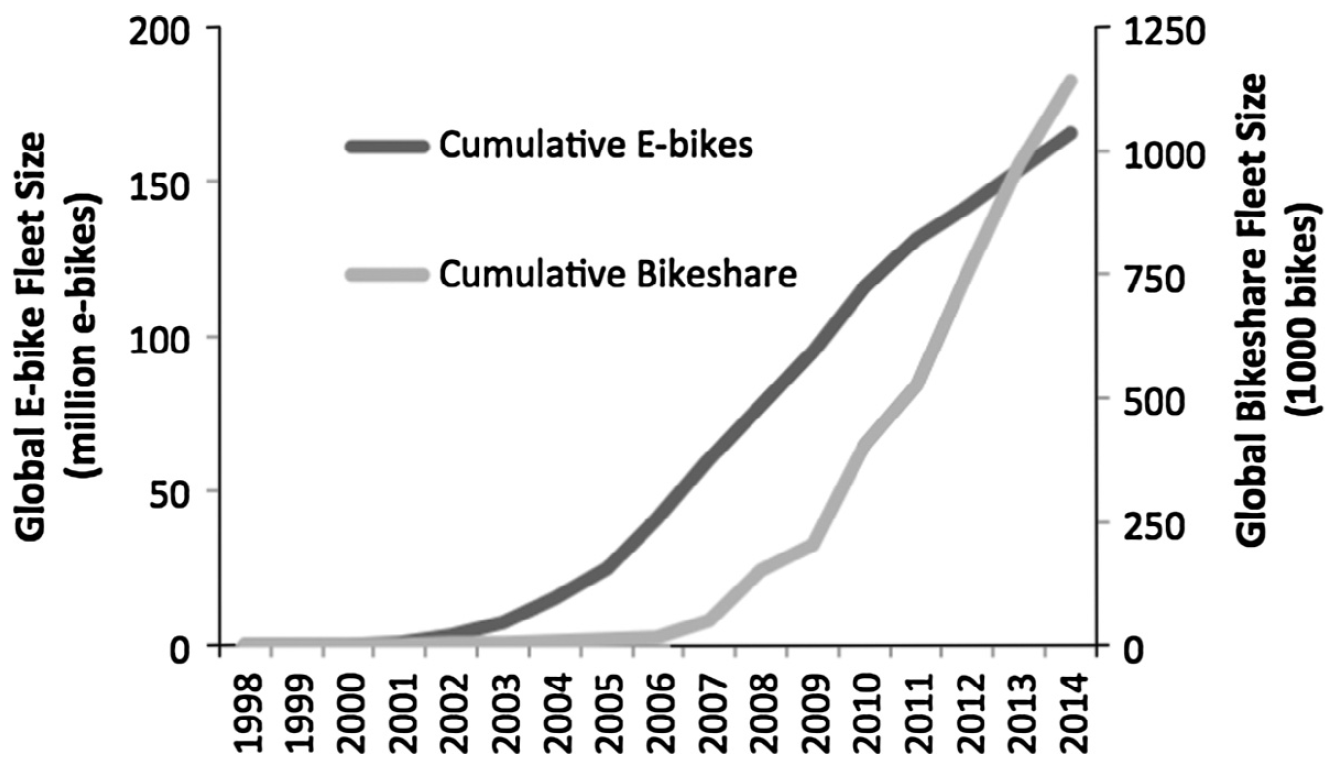
\includegraphics[width=0.6\linewidth]{image/bike_sharing} \caption{Growth in personal e-bike and public bikeshare systems (Campbell et al., 2016)}\label{fig:unnamed-chunk-7}
\end{figure}

Private BSS operators from China (\emph{Mobike, Ofo}) and Shanghai (\emph{oBike}) are currently introducing large fleets of station-less rental bikes in cities worldwide. The roll-out, especially in European cities, has encountered problems as city governments have not been able to coordinate the introduction (Zademach and Musch, 2018). Many bikes have been found abandoned around the cities. In addition, there are fears in some cases that the private companies introduced the BSS with the sole reason of tapping into private user data (Schöffel et al., 2017).
Furthermore, the company Montreal introduced ``BIXI'', fixed, portable, solar-powered and modular stations. They are self-contained and the stations can be placed, moved and relocated to desired locations within 20 minutes. ``Mega'' docking stations are available for special events (Midgley, 2011).
The number of BSSs has grown to over 800 units worldwide (Fishman, 2016). The public-private partnership model has been the most widespread, and the implementation of BSSs has been possible in cities with limited public funds (Zademach and Musch, 2018).
In Austria, there are multiple companies currently offering bicycle or e-bicycle sharing services such as \emph{Citybike, Ofo or oBike}. Nevertheless, about a year after their launch, the Asian providers of stationless rental bikes in Vienna (start-ups \emph{Ofo} and \emph{oBike}) have been in retreat from the federal capital (Rachbauer, 2018b). This has been a result of strict rules with respect to stationless rental bikes in Vienna announced on 1st August 2018. A failure to comply with the rules resulted in the bikes being removed for a fee. Previously, the traffic road act (\emph{StVO}) allowed the placement of rental bikes in public spaces and the city lacked the means of action against the providers. With the help of a so-called local police ordinance, the city hall required that the bike-sharing companies pick up objectionable bikes on weekdays within four hours and at night and on weekends within twelve hours after notification. If they did not comply, the bikes were removed for a fee. In addition, administrative fines of up to 700 euros were possible. Moreover, a limit of maximum 1500 bicycles per provider was also set. Now, the bikes are given a number and each one has to be registered with the city. According to Blum, setting up several companies to circumvent the upper limit is not allowed. The rental companies themselves also have to meet certaine criteria, for instance, there must be a company headquarters in Vienna and a service hotline. \emph{Ofo} and \emph{oBike} already meet these requirements (Rachbauer, 2018d).
Across Austria the situation with rental bikes differs significantly, for example in Innsbruck, renatal bikes were first introduced in 2014 and and are succesfully opearting. Meanwhile, in Linz rental bike system has been approved in 2017 and the docking stations are currently under construction. Further, in Salzburg the S-Bike rental system is operating and linked to federal funding (Affenzeller, 2020, Citybike Salzburg, no date a). On the other hand in Graz there is no uniform bike rental system and these services are provided by shops and hotels (Rachbauer, 2016).

\hypertarget{relevant-initiatives-in-austria-32}{%
\subsection*{Relevant initiatives in Austria}\label{relevant-initiatives-in-austria-32}}
\addcontentsline{toc}{subsection}{Relevant initiatives in Austria}

\begin{itemize}
\tightlist
\item
  \href{https://www.citybikewien.at/de}{citybikewien}
\item
  \href{http://www.citybikesalzburg.at/}{citybikesalzburg}
\item
  \href{https://www.nextbike.at/de/niederoesterreich/}{nextbike}
\item
  \href{https://www.tips.at/nachrichten/linz/land-leute/523512-linzer-radverleih-startet-im-fruehjahr-an-40-standorten}{tpis.at}
\end{itemize}

\hypertarget{impacts-with-respect-to-sustainable-development-goals-sdgs-32}{%
\subsection*{Impacts with respect to Sustainable Development Goals (SDGs)}\label{impacts-with-respect-to-sustainable-development-goals-sdgs-32}}
\addcontentsline{toc}{subsection}{Impacts with respect to Sustainable Development Goals (SDGs)}

\begin{longtable}[]{@{}ccccc@{}}
\toprule
\begin{minipage}[b]{0.17\columnwidth}\centering
Impact level\strut
\end{minipage} & \begin{minipage}[b]{0.16\columnwidth}\centering
Indicator\strut
\end{minipage} & \begin{minipage}[b]{0.17\columnwidth}\centering
Impact direction\strut
\end{minipage} & \begin{minipage}[b]{0.17\columnwidth}\centering
Goal description and number\strut
\end{minipage} & \begin{minipage}[b]{0.17\columnwidth}\centering
Source\strut
\end{minipage}\tabularnewline
\midrule
\endhead
\begin{minipage}[t]{0.17\columnwidth}\centering
Individual\strut
\end{minipage} & \begin{minipage}[t]{0.16\columnwidth}\centering
Often first 30-60 minutes free of charge\strut
\end{minipage} & \begin{minipage}[t]{0.17\columnwidth}\centering
\textbf{+}\strut
\end{minipage} & \begin{minipage}[t]{0.17\columnwidth}\centering
Equality (\emph{5,10})\strut
\end{minipage} & \begin{minipage}[t]{0.17\columnwidth}\centering
Citybike Salzburg, no date b; Citybike Wien, no date; Nextbike Niederoesterreich, no date\strut
\end{minipage}\tabularnewline
\begin{minipage}[t]{0.17\columnwidth}\centering
Individual\strut
\end{minipage} & \begin{minipage}[t]{0.16\columnwidth}\centering
Continuous advancement in bike features\strut
\end{minipage} & \begin{minipage}[t]{0.17\columnwidth}\centering
\textbf{+}\strut
\end{minipage} & \begin{minipage}[t]{0.17\columnwidth}\centering
Innovation \& Infrastructure (\emph{9})\strut
\end{minipage} & \begin{minipage}[t]{0.17\columnwidth}\centering
Zademach \& Musch, 2018\strut
\end{minipage}\tabularnewline
\begin{minipage}[t]{0.17\columnwidth}\centering
Systemic\strut
\end{minipage} & \begin{minipage}[t]{0.16\columnwidth}\centering
Wider access to this cheap or free mobility service\strut
\end{minipage} & \begin{minipage}[t]{0.17\columnwidth}\centering
\textbf{+}\strut
\end{minipage} & \begin{minipage}[t]{0.17\columnwidth}\centering
Equality (\emph{5,10})\strut
\end{minipage} & \begin{minipage}[t]{0.17\columnwidth}\centering
El Arbi \& Stephane, 2020\strut
\end{minipage}\tabularnewline
\begin{minipage}[t]{0.17\columnwidth}\centering
Systemic\strut
\end{minipage} & \begin{minipage}[t]{0.16\columnwidth}\centering
Air pollution, noise pollution and congestion reduced\strut
\end{minipage} & \begin{minipage}[t]{0.17\columnwidth}\centering
\textbf{+}\strut
\end{minipage} & \begin{minipage}[t]{0.17\columnwidth}\centering
Environmental sustainability (\emph{7,12,13,15})\strut
\end{minipage} & \begin{minipage}[t]{0.17\columnwidth}\centering
El Arbi \& Stephane, 2020\strut
\end{minipage}\tabularnewline
\begin{minipage}[t]{0.17\columnwidth}\centering
Systemic\strut
\end{minipage} & \begin{minipage}[t]{0.16\columnwidth}\centering
Investment in bike sharing infrastructure\strut
\end{minipage} & \begin{minipage}[t]{0.17\columnwidth}\centering
\textbf{+}\strut
\end{minipage} & \begin{minipage}[t]{0.17\columnwidth}\centering
Innovation \& Infrastructure (\emph{9})\strut
\end{minipage} & \begin{minipage}[t]{0.17\columnwidth}\centering
der Grazer, 2019; Hillebrand, 2019; Affenzeller, 2020; Tech \& Nature, 2020\strut
\end{minipage}\tabularnewline
\begin{minipage}[t]{0.17\columnwidth}\centering
Systemic\strut
\end{minipage} & \begin{minipage}[t]{0.16\columnwidth}\centering
48\% of all systems are operated as public-private partnerships\strut
\end{minipage} & \begin{minipage}[t]{0.17\columnwidth}\centering
\textbf{+}\strut
\end{minipage} & \begin{minipage}[t]{0.17\columnwidth}\centering
Partnership \& collaborations (\emph{17})\strut
\end{minipage} & \begin{minipage}[t]{0.17\columnwidth}\centering
Midgley, 2011\strut
\end{minipage}\tabularnewline
\bottomrule
\end{longtable}

\hypertarget{technology-and-societal-readiness-level-32}{%
\subsection*{Technology and societal readiness level}\label{technology-and-societal-readiness-level-32}}
\addcontentsline{toc}{subsection}{Technology and societal readiness level}

\begin{longtable}[]{@{}cc@{}}
\toprule
TRL & SRL\tabularnewline
\midrule
\endhead
7-9 & 5-7\tabularnewline
\bottomrule
\end{longtable}

\hypertarget{open-questions-32}{%
\subsection*{Open questions}\label{open-questions-32}}
\addcontentsline{toc}{subsection}{Open questions}

\begin{enumerate}
\def\labelenumi{\arabic{enumi}.}
\tightlist
\item
  What measures can be implemented to tackle the vandalism of the bikes?
\item
  Which bike system (docked vs.~free-floating) is more sustainable in the long-term?
\end{enumerate}

\hypertarget{further-links-27}{%
\subsection*{Further links}\label{further-links-27}}
\addcontentsline{toc}{subsection}{Further links}

\begin{itemize}
\tightlist
\item
  \href{http://en.cyclocity.com/}{cyclocity.com}
\end{itemize}

\hypertarget{references-32}{%
\subsection*{References}\label{references-32}}
\addcontentsline{toc}{subsection}{References}

\begin{itemize}
\tightlist
\item
  Affenzeller, J. (2020, December 17). Linzer Radverleih startet im Frühjahr an 40 Standorten. \url{https://www.tips.at/nachrichten/linz/land-leute/523512-linzer-radverleih-startet-im-fruehjahr-an-40-standorten}
\item
  Campbell, A. A., Cherry, C. R., Ryerson, M. S., \& Yang, X. (2016). Factors influencing the choice of shared bicycles and shared electric bikes in Beijing. Transportation Research Part C: Emerging Technologies, 67, 399--414. \url{https://doi.org/10.1016/j.trc.2016.03.004}
\item
  Cheng, L., Yang, J., Chen, X., Cao, M., Zhou, H., \& Sun, Y. (2020). How could the station-based bike sharing system and the free-floating bike sharing system be coordinated? Journal of Transport Geography, 89(March 2019), 102896. \url{https://doi.org/10.1016/j.jtrangeo.2020.102896}
\item
  Cheng, X., \& Gao, Y. (2018). The Optimal Monthly Strategy Pricing of Free-Floating Bike Sharing Platform. Modern Economy, 09(02), 318--338. \url{https://doi.org/10.4236/me.2018.92021}
\item
  Citybike Salzburg. (n.d.-a). Citybike Salzburg. Retrieved 12 January 2021, from \url{http://www.citybikesalzburg.at/hanuschplatz.php}
\item
  Citybike Salzburg. (n.d.-b). Citybike Salzburg - Tarife. Retrieved 18 January 2021, from \url{http://www.citybikesalzburg.at/tarife.php}
\item
  Citybike Wien. (n.d.). Tarife - Citybike Wien. Retrieved 18 January 2021, from \url{https://www.citybikewien.at/de/tarife}
\item
  Citybike Wien. (2019). 10 Millionen Fahrten bei Citybike Wien! \url{https://www.citybikewien.at/de/news/595-neuer-meilenstein-bei-citybike-wien-erreicht}
\item
  DeMaio, P. (2009). Bike-sharing: History, Impacts, Models of Provision, and Future. Journal of Public Transportation, 12(4), 41--56. \url{https://doi.org/10.5038/2375-0901.12.4.3}
\item
  der Grazer. (2019, October 21). 100 Millionen Euro für Fahrrad-Offensive im Großraum Graz -- Der Grazer. \url{https://grazer.at/de/uHAnk5t2/100-millionen-euro-fuer-fahrrad-offensive-im-graz/}
\item
  Eillie, A. (2016). Oxford Test Drives Peer-to-Peer Bike Sharing. \url{https://www.bloomberg.com/news/articles/2016-09-13/cycle-land-is-a-new-peer-to-peer-bike-sharing-platform}
\item
  El Arbi, A. A., \& Stephane, C. K. T. (2020). Intelligent Management of Bike Sharing in Smart Cities using Machine Learning and Internet of Things. Sustainable Cities and Society, 135907. \url{https://doi.org/10.1016/j.scs.2020.102702}
\item
  Fishman, E. (2016). Bikeshare: A Review of Recent Literature. Transport Reviews, 36(1), 92--113. \url{https://doi.org/10.1080/01441647.2015.1033036}
\item
  Fishman, E., Washington, S., Haworth, N., \& Mazzei, A. (2014). Barriers to bikesharing: An analysis from Melbourne and Brisbane. Journal of Transport Geography, 41, 325--337. \url{https://doi.org/10.1016/j.jtrangeo.2014.08.005}
\item
  Gu, T., Kim, I., \& Currie, G. (2019). To be or not to be dockless: Empirical analysis of dockless bikeshare development in China. Transportation Research Part A: Policy and Practice, 119, 122--147. \url{https://doi.org/10.1016/j.tra.2018.11.007}
\item
  Hillebrand, T. (2019). Mietradsystem `Stadtrad Innsbruck' - VCÖ Vorbildhafte Mobilitätsprojekte. \url{https://mobilitaetsprojekte.vcoe.at/mietradsystem-stadtrad-innsbruck-2019}
\item
  Li, H., Zhang, Y., Ding, H., \& Ren, G. (2019). Effects of dockless bike-sharing systems on the usage of the London Cycle Hire. Transportation Research Part A: Policy and Practice, 130, 398--411. \url{https://doi.org/10.1016/j.tra.2019.09.050}
\item
  Ma, X., Ji, Y., Yuan, Y., Van Oort, N., Jin, Y., \& Hoogendoorn, S. (2020). A comparison in travel patterns and determinants of user demand between docked and dockless bike-sharing systems using multi-sourced data. Transportation Research Part A: Policy and Practice, 139(June), 148--173. \url{https://doi.org/10.1016/j.tra.2020.06.022}
\item
  Midgley, P. (2011). Bicycle-Sharing Schemes: Enhancing Sustainable Mobility in Urban Areas. Commission on Sustainable Development, Nine teent(8), 24. \url{http://www.un.org/esa/dsd/resources/res_pdfs/csd-19/Background-Paper8-P.Midgley-Bicycle.pdf}
\item
  Nextbike Niederösterreich. (n.d.). Nextbike Niederösterreich - Tarife. Retrieved 18 January 2021, from \url{https://www.nextbike.at/de/niederoesterreich/preise/}
\item
  Rachbauer, S. (2016, July). Bikesharing in Österreich: Leihräder auf der Überholspur \textbar{} kurier.at. \url{https://kurier.at/chronik/oesterreich/bikesharing-in-oesterreich-leihraeder-auf-der-ueberholspur/400067369}
\item
  Rachbauer, S. (2018a). Bikesharing in Österreich: Leihräder auf der Überholspur. \url{https://kurier.at/chronik/oesterreich/bikesharing-in-oesterreich-leihraeder-auf-der-ueberholspur/400067369}
\item
  Rachbauer, S. (2018b). Leihräder: Wiener wollen es aufgeräumt. \url{https://kurier.at/chronik/wien/leihraeder-wiener-wollen-es-aufgeraeumt/400067357}
\item
  Rachbauer, S. (2018c, March). Wien führt strenge Regeln für stationslose Leihräder ein. \url{https://kurier.at/chronik/wien/wien-fuehrt-strenge-regeln-fuer-stationslose-leihraeder-ein/312.944.617}
\item
  Rachbauer, S. (2018d, July 17). Leihräder: Wiener wollen es aufgeräumt. \url{https://kurier.at/chronik/wien/leihraeder-wiener-wollen-es-aufgeraeumt/400067357}
\item
  Schöffel, R., Zierer, M., \& Kühne, S. (2017). Nutzerdaten offen im Netz: BR deckt Datenleck beim Fahrradverleiher Obike auf. \url{https://www.br.de/nachricht/datenleck-obike-100.html}
\item
  Sun, S., \& Ertz, M. (2021). Contribution of bike-sharing to urban resource conservation: The case of free-floating bike-sharing. Journal of Cleaner Production, 280, 124416. \url{https://doi.org/10.1016/j.jclepro.2020.124416}
\item
  Tech \& Nature. (2020, April 28). Niederösterreich modernisiert Sharing-Bike-Flotte `nextbike' - Tech \& Nature. \url{https://www.techandnature.com/niederosterreich-modernisiert-sharing-bike-flotte-nextbike/}
\item
  Zademach, H. M., \& Musch, A. K. (2018). Bicycle-sharing systems in an alternative/diverse economy perspective: a sympathetic critique. Local Environment, 23(7), 734--746. \url{https://doi.org/10.1080/13549839.2018.1434494}
\item
  Zhang, Y., Lin, D., \& Mi, Z. (2019). Electric fence planning for dockless bike-sharing services. Journal of Cleaner Production, 206, 383--393. \url{https://doi.org/10.1016/j.jclepro.2018.09.215}
\end{itemize}

\hypertarget{scooters}{%
\section{E-scooters}\label{scooters}}

\hypertarget{synonyms-29}{%
\subsection*{Synonyms}\label{synonyms-29}}
\addcontentsline{toc}{subsection}{Synonyms}

\emph{electric scooter}

\hypertarget{definition-33}{%
\subsection*{Definition}\label{definition-33}}
\addcontentsline{toc}{subsection}{Definition}

E-scooters are electrically powered scooters which move at a similar speed to bicycles. They are one of micro-mobility solutions which is growing trend in urban mobility. It encompasses all human-powered micro-vehicles, such as bicycles and scooters, but also new micro-vehicles such as e-scooters, e-bikes and some other small, electrically powered vehicles (Oeschger, Carroll and Caulfield, 2020). Most of the modern vehicles of this type are available for both shared and private use and are gaining wide acceptance.
E-scooters have promised a solution to the last mile problem since their introduction in 2017 (Siegfried et al, 2021). They are seen as alternatives to cars and provide potential for reducing traffic congestion, noise and pollution. Initial results suggest that e-scooters are mainly used for distances between 1 and 6 km. Empirical evidence shows that e-scooters can substitute walking rather than driving for these short distances (James et al., 2019; Portland Bureau of Transportation, 2019). In addition to the potential positive environmental impact of e-scooters on the transportation system, some safety concerns have been raised. Most e-scooter users who had an accident have ridden without a helmet (Liew et al, 2020). In general, e-scooters are almost exclusively issued without protective equipment (Allem and Majmundar, 2019). The safety issues do not only affect the riders themselves, but also have an impact on other road users, especially pedestrians (Sikka et al., 2019). It has even been criticised that technology follows the idea of ``sell first, safety later'' (Choron and Sakran, 2019).

\hypertarget{key-stakeholders-33}{%
\subsection*{Key stakeholders}\label{key-stakeholders-33}}
\addcontentsline{toc}{subsection}{Key stakeholders}

\begin{itemize}
\tightlist
\item
  \textbf{Affected}: Mobile citizens, pedestrians, insurers
\item
  \textbf{Responsible}: National governments, city government, private Companies
\end{itemize}

\hypertarget{current-state-of-art-in-research-33}{%
\subsection*{Current state of art in research}\label{current-state-of-art-in-research-33}}
\addcontentsline{toc}{subsection}{Current state of art in research}

Since e-scooters are already well-established technology, most research focuses on safety and accidents, user behaviour and potential environmental impact of uptake of this micro-mobility option. Some studies advocate e-scooters as an environmentally friendly solution for crowded cities, others report contradictory results and point to safety issues.
Moreover, research also explores whether the presence of e-scooters reduces bicycle thefts (Gössling, 2020). In Gothenburg, Sweden, the police reported that the number of bicycle thefts halved after the introduction of e-scooters and rental bikes (Sydsvenskan, 2019).

\hypertarget{current-state-of-art-in-practice-32}{%
\subsection*{Current state of art in practice}\label{current-state-of-art-in-practice-32}}
\addcontentsline{toc}{subsection}{Current state of art in practice}

E-scooter providers such as \emph{Lime} and \emph{Bird}, which launched operations in California in 2017, can now be found in over 100 cities worldwide and have since recorded millions of rides. E-scooter provider \emph{VOI} has experienced similar growth in Europe and entered the market in 10 countries in just one year after launching in Sweden and has recorded over 16 million rides (Oeschger et al., 2020). The results of a survey indicate that e-scooters are primarily seen as entertainment and not as a means of transport (Siegfried et al., 2021).
Maximum speed limits are an important issue and internationally there are different approaches. Los Angeles and Dallas, for example, have no speed limit, as far as can be deduced from the news; while the limit in Vienna is 25 km/h (Schwarz, 2019). Paris is discussing reducing the speed limit to 20 km/h on cycle paths and 8 km/h in parks and pedestrian areas (Négroni, 2019). One problem with the maximum speeds is that some of the e-scooter models can go much faster than 25 km/h (Le Figaro, 2018). To counteract the negative consequences of the introduction of e-scooters, cities have evaluated and implemented various rules and guidelines. Media analysis suggests that the city councils should introduce the following rules as a minimal requirement: speed limits, restrictions on the exclusive use of bicycle infrastructure and a designation of parking spaces for rental and return. Behavioural campaigns and fines, are needed to limit negative consequences of e-scooter use (Gössling, 2020).
In Vienna, only very few e-scooters are used on bicycle paths (between 4.9\% and 7.1\% compared to other bicycle path users). Given the modal split of Vienna (7\% cycling), it can be concluded that e-scooters do not yet have a significant role in Vienna's transport system (Laa and Leth, 2020).

\hypertarget{relevant-initiatives-in-austria-33}{%
\subsection*{Relevant initiatives in Austria}\label{relevant-initiatives-in-austria-33}}
\addcontentsline{toc}{subsection}{Relevant initiatives in Austria}

\begin{itemize}
\tightlist
\item
  \href{https://autorevue.at/ratgeber/e-scooter-wien-vergleich}{autorevue.at}
\item
  \href{https://www.stadt-wien.at/wien/news/e-scooter-sharing-system-in-wien.html}{stadt-wien.at}
\item
  \href{https://www.wien.gv.at/verkehr/scooter-roller/index.html}{wien.gv.at}
\item
  \href{https://www.oeamtc.at/thema/fahrrad/e-kleintretroller-e-scooter-in-oesterreich-31721872}{oeamtc.at}
\item
  \href{https://www.oesterreich.gv.at/themen/freizeit_und_strassenverkehr/Elektro-Scooter,-Quads-und-Co/Seite.610110.html}{oesterreich.gv.at}
\end{itemize}

\hypertarget{impacts-with-respect-to-sustainable-development-goals-sdgs-33}{%
\subsection*{Impacts with respect to Sustainable Development Goals (SDGs)}\label{impacts-with-respect-to-sustainable-development-goals-sdgs-33}}
\addcontentsline{toc}{subsection}{Impacts with respect to Sustainable Development Goals (SDGs)}

\begin{longtable}[]{@{}ccccc@{}}
\toprule
\begin{minipage}[b]{0.17\columnwidth}\centering
Impact level\strut
\end{minipage} & \begin{minipage}[b]{0.16\columnwidth}\centering
Indicator\strut
\end{minipage} & \begin{minipage}[b]{0.17\columnwidth}\centering
Impact direction\strut
\end{minipage} & \begin{minipage}[b]{0.17\columnwidth}\centering
Goal description and number\strut
\end{minipage} & \begin{minipage}[b]{0.17\columnwidth}\centering
Source\strut
\end{minipage}\tabularnewline
\midrule
\endhead
\begin{minipage}[t]{0.17\columnwidth}\centering
Individual\strut
\end{minipage} & \begin{minipage}[t]{0.16\columnwidth}\centering
E-scooter trips replace mainly walking trips\strut
\end{minipage} & \begin{minipage}[t]{0.17\columnwidth}\centering
\textbf{-}\strut
\end{minipage} & \begin{minipage}[t]{0.17\columnwidth}\centering
Health \& Wellbeing (\emph{3})\strut
\end{minipage} & \begin{minipage}[t]{0.17\columnwidth}\centering
Laa \& Leth, 2020\strut
\end{minipage}\tabularnewline
\begin{minipage}[t]{0.17\columnwidth}\centering
Individual\strut
\end{minipage} & \begin{minipage}[t]{0.16\columnwidth}\centering
More expensive compared to public transport\strut
\end{minipage} & \begin{minipage}[t]{0.17\columnwidth}\centering
\textbf{-}\strut
\end{minipage} & \begin{minipage}[t]{0.17\columnwidth}\centering
Sustainable economic development (\emph{8,11})\strut
\end{minipage} & \begin{minipage}[t]{0.17\columnwidth}\centering
Widholm, 2021; Wiener Linien, 2021\strut
\end{minipage}\tabularnewline
\begin{minipage}[t]{0.17\columnwidth}\centering
Individual\strut
\end{minipage} & \begin{minipage}[t]{0.16\columnwidth}\centering
Increase in participants on existing road infrastructure\strut
\end{minipage} & \begin{minipage}[t]{0.17\columnwidth}\centering
\textbf{\textasciitilde{}}\strut
\end{minipage} & \begin{minipage}[t]{0.17\columnwidth}\centering
Innovation \& Infrastructure (\emph{9})\strut
\end{minipage} & \begin{minipage}[t]{0.17\columnwidth}\centering
Laa \& Leth, 2020\strut
\end{minipage}\tabularnewline
\begin{minipage}[t]{0.17\columnwidth}\centering
Systemic\strut
\end{minipage} & \begin{minipage}[t]{0.16\columnwidth}\centering
Highest user share among young males\strut
\end{minipage} & \begin{minipage}[t]{0.17\columnwidth}\centering
\textbf{-}\strut
\end{minipage} & \begin{minipage}[t]{0.17\columnwidth}\centering
Equality (\emph{5,10})\strut
\end{minipage} & \begin{minipage}[t]{0.17\columnwidth}\centering
Laa \& Leth, 2020\strut
\end{minipage}\tabularnewline
\begin{minipage}[t]{0.17\columnwidth}\centering
Systemic\strut
\end{minipage} & \begin{minipage}[t]{0.16\columnwidth}\centering
E-scooter trips repalce more sustainable transport modes\strut
\end{minipage} & \begin{minipage}[t]{0.17\columnwidth}\centering
\textbf{-}\strut
\end{minipage} & \begin{minipage}[t]{0.17\columnwidth}\centering
Environmental sustainability (\emph{7,12,13,15})\strut
\end{minipage} & \begin{minipage}[t]{0.17\columnwidth}\centering
Laa \& Leth, 2020\strut
\end{minipage}\tabularnewline
\begin{minipage}[t]{0.17\columnwidth}\centering
Systemic\strut
\end{minipage} & \begin{minipage}[t]{0.16\columnwidth}\centering
Growth in micromobility sector\strut
\end{minipage} & \begin{minipage}[t]{0.17\columnwidth}\centering
\textbf{+}\strut
\end{minipage} & \begin{minipage}[t]{0.17\columnwidth}\centering
Sustainable economic development (\emph{8,11})\strut
\end{minipage} & \begin{minipage}[t]{0.17\columnwidth}\centering
Goessling, 2020\strut
\end{minipage}\tabularnewline
\bottomrule
\end{longtable}

\hypertarget{technology-and-societal-readiness-level-33}{%
\subsection*{Technology and societal readiness level}\label{technology-and-societal-readiness-level-33}}
\addcontentsline{toc}{subsection}{Technology and societal readiness level}

\begin{longtable}[]{@{}cc@{}}
\toprule
TRL & SRL\tabularnewline
\midrule
\endhead
7-9 & 7-9\tabularnewline
\bottomrule
\end{longtable}

\hypertarget{open-questions-33}{%
\subsection*{Open questions}\label{open-questions-33}}
\addcontentsline{toc}{subsection}{Open questions}

\begin{enumerate}
\def\labelenumi{\arabic{enumi}.}
\tightlist
\item
  Will an increasing presence of e-scooters on the bicycle infrastructure or in pedestrian zones require separate solution in urban road infrastructure?
\end{enumerate}

\hypertarget{references-33}{%
\subsection*{References}\label{references-33}}
\addcontentsline{toc}{subsection}{References}

\begin{itemize}
\tightlist
\item
  Allem, J. P., \& Majmundar, A. (2019). Are electric scooters promoted on social media with safety in mind? A case study on Bird's Instagram. In Preventive Medicine Reports (Vol. 13, pp.~62--63). Elsevier Inc.~\url{https://doi.org/10.1016/j.pmedr.2018.11.013}
\item
  Choron, R. L., \& Sakran, J. V. (2019). The Integration of Electric Scooters: Useful Technology or Public Health Problem? American Journal of Public Health, 109(4), 555--556. \url{https://doi.org/10.2105/AJPH.2019.304955}
\item
  Gössling, S. (2020). Integrating e-scooters in urban transportation: Problems, policies, and the prospect of system change. Transportation Research Part D: Transport and Environment, 79(January), 102230. \url{https://doi.org/10.1016/j.trd.2020.102230}
\item
  James, O., Swiderski, J., Hicks, J., Teoman, D., \& Buehler, R. (2019). Pedestrians and E-Scooters: An Initial Look at E-Scooter Parking and Perceptions by Riders and Non-Riders. Sustainability, 11(20), 5591. \url{https://doi.org/10.3390/su11205591}
\item
  Laa, B., \& Leth, U. (2020). Survey of E-scooter users in Vienna: Who they are and how they ride. Journal of Transport Geography, 89(October), 102874. \url{https://doi.org/10.1016/j.jtrangeo.2020.102874}
\item
  Le Figaro. (2018, September 9). Trottinettes: la mairie de Paris veut une réglementation nationale. \url{https://www.lefigaro.fr/flash-eco/2018/09/09/97002-20180909FILWWW00064-trottinettes-la-mairie-de-paris-veut-une-reglementation-nationale.php}
\item
  Liew, Y. K., Wee, C. P. J., \& Pek, J. H. (2020). New peril on our roads: A retrospective study of electric scooter-related injuries. Singapore Medical Journal, 61(2), 92--95. \url{https://doi.org/10.11622/smedj.2019083}
\item
  Négroni, A. (2019, June 6). Paris: Hidalgo prend des mesures contre les trottinettes électriques. \url{https://www.lefigaro.fr/actualite-france/trottinettes-paris-prend-des-mesures-20190606}
\item
  OECD/ITF. (2020). Safe Micromobility. 98. \url{https://www.itf-oecd.org/safe-micromobility}
\item
  Oeschger, G., Carroll, P., \& Caulfield, B. (2020). Micromobility and public transport integration: The current state of knowledge. Transportation Research Part D: Transport and Environment, 89, 102628. \url{https://doi.org/10.1016/j.trd.2020.102628}
\item
  Portland Bureau of Transportation. (2019). 2018 E-Scooter Findings Report. \url{https://www.portlandoregon.gov/transportation/article/709719\%0Ahttps://trid.trb.org/view/1607260}
\item
  Schwarz, R. (2019, July 27). E-Bikes und E-Scooter sind viel zu schnell! - Ideen-Blog - derStandard.at › Diskurs. \url{https://www.derstandard.at/story/2000106514149/e-bikes-und-e-scooter-sind-viel-zu-schnell}
\item
  Siegfried, C., Martin, B., \& Reichenberger, Y. (2021). Consumer acceptance of shared e-scooters for urban and short-distance mobility. Transportation Research Part D, 91(January), 102680. \url{https://doi.org/10.1016/j.trd.2020.102680}
\item
  Sikka, N., Vila, C., Stratton, M., Ghassemi, M., \& Pourmand, A. (2019). Sharing the sidewalk: A case of E-scooter related pedestrian injury. American Journal of Emergency Medicine, 37(9), 1807.e5-1807.e7. \url{https://doi.org/10.1016/j.ajem.2019.06.017}
\item
  Sydsvenskan. (2019, August 30). Elsparkcyklarna minskar cykelstölderna - Sydsvenskan. \url{https://www.sydsvenskan.se/2019-08-30/elsparkcyklarna-minskar-cykelstolderna}
\item
  Widholm, K. (n.d.). E-Scooter Sharing-System: Roller von Lime, Tier, Bird und Co.~Retrieved 20 January 2021, from \url{https://www.stadt-wien.at/wien/news/e-scooter-sharing-system-in-wien.html}
\item
  Wiener Linien. (n.d.). Übersicht Tickets \textbar{} Tickets \textbar{} Fahrgastinfo \textbar{} Wiener Linien. Retrieved 20 January 2021, from \url{https://www.wienerlinien.at/eportal3/ep/channelView.do/pageTypeId/66526/channelId/-46648}
\item
  Zagorskas, J., \& Burinskiene, M. (2020). Challenges caused by increased use of E-powered personal mobility vehicles in European cities. Sustainability (Switzerland), 12(1), 273. \url{https://doi.org/10.3390/su12010273}
\end{itemize}

\hypertarget{ride_hailing}{%
\section{Ride-hailing \& Ride-sharing}\label{ride_hailing}}

\hypertarget{synonyms-30}{%
\subsection*{Synonyms}\label{synonyms-30}}
\addcontentsline{toc}{subsection}{Synonyms}

\begin{itemize}
\tightlist
\item
  Ride hailing: \emph{Ridesourcing, app-based ride services, ride-booking, on-demand ride services, Transportation Network Companies (TNCs), mobility service providers (MSPs)}
\item
  Ride sharing: \emph{car-pooling}
\end{itemize}

\hypertarget{definition-34}{%
\subsection*{Definition}\label{definition-34}}
\addcontentsline{toc}{subsection}{Definition}

Ride sharing and ride hailing both emerged from the ``shared economy'' or ``collaborative economy'', which aims to share underutilized resources to increase efficiency, protect the environment and promote economic growth (Tirachini, 2019).

Ride hailing (RH) in comparison to street-hailing enables booking a journey via an online platform -- usually an app. The platforms match travellers who want to book a specific ride with a personal driver who is willing to take that ride in their private car, based on their location. Ride-hailing platforms mostly eliminate the exchange of cash and apply basic economic principles to match supply and demand through dynamic price adjustments. However, this original model is not allowed in all countries. In Austria, for example, it is not allowed to offer ride hailing with one's private car, only with rental cars. Since 2021, drivers are also required to have a Viennese taxi driver's license (Uber Technologies Inc., n.d.).

Ride sharing, by contrast, describes the process in which a rider shares a vehicle with multiple other riders, who want to go in the same direction. Some Transportation Network Companies who offer ride hailing are also offering ride sharing services, like \emph{UberPool} or \emph{Lyft Shared} which are usually cheaper and also more environmentally friendly due to the higher occupancy rate (Herzog, 2018). Dynamic ride sharing systems use algorithms to match riders, who want to go in a similar direction and form a shared ride (Lokhandwala \& Cai, 2018).

\hypertarget{key-stakeholders-34}{%
\subsection*{Key stakeholders}\label{key-stakeholders-34}}
\addcontentsline{toc}{subsection}{Key stakeholders}

\begin{itemize}
\tightlist
\item
  \textbf{Affected}: Mobile Citizen, Taxi Drivers
\item
  \textbf{Responsible}: National Governments, City government, Private Companies, Transportation Network Companies, Software providers
\end{itemize}

\hypertarget{current-state-of-art-in-research-34}{%
\subsection*{Current state of art in research}\label{current-state-of-art-in-research-34}}
\addcontentsline{toc}{subsection}{Current state of art in research}

Even though ride hailing emerged from the sharing economy, it is controversial whether it has ultimately had a positive effect on the environment (Herzog, 2018).

Jan et al.~(2018) argue that ride hailing has a positive impact on economic efficiency. As it both complements and competes with public transport, its impact on congestion near city centres is still unclear. In terms of equity, ride hailing reinforces the problem of the digital gap and raises concerns about discrimination, privacy and security. It is also controversial whether prosumers (producers/consumers) are exploited by sharing economy platforms, whether ride hailing drivers are adequately compensated and how the rights of on-demand workers can be better protected. Even though ride hailing likes to present itself with a green image, the actual environmental impacts have not yet been thoroughly investigated. Further, Jin et al.~(2018) pointed out the danger of conceptual confusion in ride hailing research. Based on evidences reported in the literature, they argue, that it is unlikely, that people stop owning cars due to ride hailing.

Regarding ride sharing, Alisoltani et al.~(2012) argue, that it can reduce traffic congestion, but only if the trip density is high, which is usually the case in large-scale networks. In smaller cities, with a small- or medium-scale network, the trip density is not high enough. Importantly, trip density is defined as the total number of trips ends (origins and destinations) within 24 h within a given area (Miller \& Soberman, 2003).

Lokhandwala \& Cai (2018) compared in a case study in New York City shared autonomous vehicles (SAVs) to traditional taxis and found out that SAVs have the potential to reduce the fleet size in NYC by more than 50\% and reduce daily greenhouse gas emissions by up to 866 MT of CO\textsubscript{2} eq.

The study by Martin et al.~(2021) provides a recent review of studies on ridesharing optimization. They compare different analytical approaches in this research area and discuss the emerging concept of ``agile'' algorithms that could help to cope with the demands of large-scale and dynamic optimization problems for ridesharing.

The NGO Mothers Against Drunk Driving (MADD) and Uber -- one of the most known ride hailing platforms -- published a report in 2015, in which they argue, based on studies in California, that the presence of uber services in a city can lower the amount of drunk driving crashes involving younger populations. Based on a study of Seattle's data, they argue that Uber's entry into the Seattle market was associated with a 10\% drop in drunk driving arrests.

\hypertarget{current-state-of-art-in-practice-33}{%
\subsection*{Current state of art in practice}\label{current-state-of-art-in-practice-33}}
\addcontentsline{toc}{subsection}{Current state of art in practice}

The two most known companies offering ride hailing in the US are \emph{Uber} and \emph{Lyft}. Uber, for instance, again offers various services, such as:

\begin{itemize}
\tightlist
\item
  UberX - affordable rides, door to door, all to yourself
\item
  UberPool - shared rides, door to door or with a short walk
\item
  UberGreen - sustainable rides in electric vehicles - or many more.
\end{itemize}

Due to regulations and uprisings of local cab companies, Uber had to adapt its business model for European cities. Other ride hailing platforms operating in Western and Central Europe are \emph{Gett, Bolt, Hailo} or \emph{Taxilo}. They all have small differences and vary based on the drivers' commission fee to the particular platform (Khatri, 2020a).

Before the Covid-19 pandemic, the ride hailing marked had been growing fast. Like other industries, the ride hailing market dropped in 2020 globally, due to the crisis and related measures, such as lockdowns, social distancing, etc. To survive, some of the bigger companies, like Uber e.g., started to foray into on-demand food delivery and parcel delivery. The industry is expected to recover depending on how quickly the general economy recovers from the crisis. Nevertheless, there will be differences in speed between countries, regions and social groups. Looking to the post-Covid era, ride hailing drivers will have to implement various safety measures, like e.g.~frequent sanitation, wearing masks, guarantee tracing, to win back the trust of customers. Mushahid Khatri (2021), a Chief Executive Officer of \href{https://www.yelowsoft.com/}{Yelowsoft} expects ``that ride-hailing companies will move towards transit authorities for providing on-demand shuttle \& bus services''. Secondly, he thinks that ride hailing companies should make sure they are part of MaaS (see section on \protect\hyperlink{maas}{MaaS}) and use Artificial Intelligence (AI) to improve their services (Khatri, 2020b).

The world's largest long-distance ride-sharing app, which has 90 million members, is \emph{BlaBlaCar}. Every quarter, 25 million global travellers use BlaBlaCar to organize their car trip and thus share the cost of travel (BlaBlaCar, 2021). Similar to other platforms based on the sharing economy, safety is ensured through a rating system where riders can rate other passengers and vice versa.

The Austrian platforms \emph{GREENDRIVE} and \emph{Carployee} both connect drivers who work for the same companies or institutions with the goal of saving company parking spaces through shared rides and protecting the environment at the same time (GREENDRIVE MOBILITY GMBH, 2020; Carployee, 2020).

\hypertarget{relevant-initiatives-in-austria-34}{%
\subsection*{Relevant initiatives in Austria}\label{relevant-initiatives-in-austria-34}}
\addcontentsline{toc}{subsection}{Relevant initiatives in Austria}

\begin{itemize}
\tightlist
\item
  \href{https://www.ots.at/presseaussendung/OTS_20210113_OTS0026/free-now-will-als-erste-mobilitaetsplattform-in-europa-bis-2030-null-emissionen-erreichen}{ots.at}
\item
  \href{https://www.umweltberatung.at/carsharing-mitfahrboersen}{umweltberatung.a}
\item
  \href{https://greendrive.at/premium/\#benefits}{greendrive.a}
\item
  \href{https://www.carployee.com/\#start-section}{carployee.com}
\item
  \href{https://ummadum.com/}{ummadum.com}
\end{itemize}

\hypertarget{impacts-with-respect-to-sustainable-development-goals-sdgs-34}{%
\subsection*{Impacts with respect to Sustainable Development Goals (SDGs)}\label{impacts-with-respect-to-sustainable-development-goals-sdgs-34}}
\addcontentsline{toc}{subsection}{Impacts with respect to Sustainable Development Goals (SDGs)}

\begin{longtable}[]{@{}ccccc@{}}
\toprule
\begin{minipage}[b]{0.17\columnwidth}\centering
Impact level\strut
\end{minipage} & \begin{minipage}[b]{0.16\columnwidth}\centering
Indicator\strut
\end{minipage} & \begin{minipage}[b]{0.17\columnwidth}\centering
Impact direction\strut
\end{minipage} & \begin{minipage}[b]{0.17\columnwidth}\centering
Goal description and number\strut
\end{minipage} & \begin{minipage}[b]{0.17\columnwidth}\centering
Source\strut
\end{minipage}\tabularnewline
\midrule
\endhead
\begin{minipage}[t]{0.17\columnwidth}\centering
Individual\strut
\end{minipage} & \begin{minipage}[t]{0.16\columnwidth}\centering
Increased accessibility\strut
\end{minipage} & \begin{minipage}[t]{0.17\columnwidth}\centering
\textbf{+}\strut
\end{minipage} & \begin{minipage}[t]{0.17\columnwidth}\centering
Equality (\emph{5,10})\strut
\end{minipage} & \begin{minipage}[t]{0.17\columnwidth}\centering
Abdelwahab, 2020; Tirachini, 2019\strut
\end{minipage}\tabularnewline
\begin{minipage}[t]{0.17\columnwidth}\centering
Systemic\strut
\end{minipage} & \begin{minipage}[t]{0.16\columnwidth}\centering
Reduced accidents by drunk drivers\strut
\end{minipage} & \begin{minipage}[t]{0.17\columnwidth}\centering
\textbf{+}\strut
\end{minipage} & \begin{minipage}[t]{0.17\columnwidth}\centering
Health \& Wellbeing (\emph{3})\strut
\end{minipage} & \begin{minipage}[t]{0.17\columnwidth}\centering
Uber \& MADD, 2015\strut
\end{minipage}\tabularnewline
\begin{minipage}[t]{0.17\columnwidth}\centering
Systemic\strut
\end{minipage} & \begin{minipage}[t]{0.16\columnwidth}\centering
Increased emissions\strut
\end{minipage} & \begin{minipage}[t]{0.17\columnwidth}\centering
\textbf{-}\strut
\end{minipage} & \begin{minipage}[t]{0.17\columnwidth}\centering
Environmental sustainability (\emph{7,12,13,15})\strut
\end{minipage} & \begin{minipage}[t]{0.17\columnwidth}\centering
Tirachini, 2019\strut
\end{minipage}\tabularnewline
\begin{minipage}[t]{0.17\columnwidth}\centering
Systemic\strut
\end{minipage} & \begin{minipage}[t]{0.16\columnwidth}\centering
Increased motorized traffic and congestion; positive impact on economic efficiency\strut
\end{minipage} & \begin{minipage}[t]{0.17\columnwidth}\centering
\textbf{\textasciitilde{}}\strut
\end{minipage} & \begin{minipage}[t]{0.17\columnwidth}\centering
Sustainable economic development (\emph{8,11})\strut
\end{minipage} & \begin{minipage}[t]{0.17\columnwidth}\centering
Tirachini, 2019; Jin et al., 2018\strut
\end{minipage}\tabularnewline
\bottomrule
\end{longtable}

\hypertarget{technology-and-societal-readiness-level-34}{%
\subsection*{Technology and societal readiness level}\label{technology-and-societal-readiness-level-34}}
\addcontentsline{toc}{subsection}{Technology and societal readiness level}

\begin{longtable}[]{@{}cc@{}}
\toprule
TRL & SRL\tabularnewline
\midrule
\endhead
7-9 & 6-9\tabularnewline
\bottomrule
\end{longtable}

\hypertarget{open-questions-34}{%
\subsection*{Open questions}\label{open-questions-34}}
\addcontentsline{toc}{subsection}{Open questions}

\begin{enumerate}
\def\labelenumi{\arabic{enumi}.}
\tightlist
\item
  How to overcome the rising concerns over discrimination and data privacy and security?
\item
  Which impacts of ride-hailing on traffic congestion outweigh the others?
\item
  How can the environmental impacts of ride hailing be reliably and holistically analysed?
\item
  How can ride-hailing and ride-sharing discourage private car ownership?
\end{enumerate}

\hypertarget{further-links-28}{%
\subsection*{Further links}\label{further-links-28}}
\addcontentsline{toc}{subsection}{Further links}

\begin{itemize}
\tightlist
\item
  \href{https://www.ots.at/presseaussendung/OTS_20210113_OTS0026/free-now-will-als-erste-mobilitaetsplattform-in-europa-bis-2030-null-emissionen-erreichen}{ots.at}
\item
  \href{https://www.umweltberatung.at/carsharing-mitfahrboersen}{umweltberatung.at}
\item
  \href{https://greendrive.at/premium/\#benefits}{greendrive}
\item
  \href{https://www.carployee.com/\#start-section}{carployee}
\item
  \href{https://ummadum.com/}{ummadum.com}
\item
  \href{https://www.blablacar.de/}{blablacar}
\item
  \href{https://www.uber.com/at/de/}{uber}
\end{itemize}

\hypertarget{references-34}{%
\subsection*{References}\label{references-34}}
\addcontentsline{toc}{subsection}{References}

\begin{itemize}
\tightlist
\item
  Abdelwahab, B. (2020). Ridesharing and Social Inclusion: The Role of Ridesharing in Improving Job Access for Disadvantaged Populations (Doctoral dissertation).
\item
  Alisoltani, N., Leclercq, L., \& Zargayouna, M. (2021). Can dynamic ride-sharing reduce traffic congestion?. Transportation research part B: methodological, 145, 212-246.
\item
  BlaBlaCar. (2021). Über uns - BlaBlaCar. \url{https://blog.blablacar.de/about-us}
\item
  Carployee. (2020). Carployee \textbar{} Für Unternehmen. \url{https://www.carployee.com/}
\item
  GREENDRIVE MOBILITY GMBH. (2020). Greendrive - Premiumpaket für Firmen - Fahrgemeinschaften und Mitfahrgelegenheiten. \url{https://greendrive.at/premium/}
\item
  Herzog, W. (2018, October 18). Ecolane Blog: Ride-hailing vs.~ride-sharing: The key difference and why it matters. \url{https://www.ecolane.com/blog/ride-hailing-vs.-ride-sharing-the-key-difference-and-why-it-matters}
\item
  Jin, S. T., Kong, H., Wu, R., \& Sui, D. Z. (2018). Ridesourcing, the sharing economy, and the future of cities. Cities, 76, 96-104.
\item
  Khatri, M. (2020a). A closer look at the ride-hailing landscape of the Western and Central Europe. \url{https://www.yelowsoft.com/blog/ride-hailing-landscape-of-western-and-central-europe/}
\item
  Khatri, M. (2020b). Ride-hailing in 2021: A glimpse into the future. \url{https://www.yelowsoft.com/blog/ride-hailing-a-glimpse-into-the-future/}
\item
  Lokhandwala, M., \& Cai, H. (2018). Dynamic ride sharing using traditional taxis and shared autonomous taxis: A case study of NYC. Transportation Research Part C: Emerging Technologies, 97, 45-60.
\item
  Martins, L. D. C., de la Torre, R., Corlu, C. G., Juan, A. A., \& Masmoudi, M. A. (2021). Optimizing ride-sharing operations in smart sustainable cities: Challenges and the need for agile algorithms. Computers \& Industrial Engineering, 153, 107080.
\item
  Miller, E., \& Soberman, R. (2003). Travel Demand.
\item
  Tirachini, A. (2019). Ride-hailing, travel behaviour and sustainable mobility: an international review. Transportation, 1-37.
\item
  Uber Technologies Inc.~(n.d.). Erhalte eine Konzession in Österreich. Retrieved March 30, 2021, from \url{https://www.uber.com/at/de/drive/requirements/get-a-license/}
\item
  Uber, \& Mothers Against Drunk Driving (MADD). (2015). MORE OPTIONS. SHIFTING MINDSETS. DRIVING BETTER CHOICES. \#ThinkandRide.
\end{itemize}

\hypertarget{alternative}{%
\chapter{Alternative power sources}\label{alternative}}

\hypertarget{FCEV}{%
\section{Hydrogen fuel cell}\label{FCEV}}

\hypertarget{synonyms-31}{%
\subsection*{Synonyms}\label{synonyms-31}}
\addcontentsline{toc}{subsection}{Synonyms}

\emph{hydrogen fuel cell electric vehicles, FCEV}

\hypertarget{definition-35}{%
\subsection*{Definition}\label{definition-35}}
\addcontentsline{toc}{subsection}{Definition}

Hydrogen Fuel Cells are systems that use hydrogen as fuel to generate electrical energy in a Fuel Cell and drive the vehicle with electrical structure. In a technical manner, they show similarities with electric vehicles. The advantages of Fuel Cell Electrical Vehicles (FCEV) are emission-free (water only), fast refuelling, noiseless driving, more economical fuel consumption and efficiency, easy maintenance. Regardless of these benefits, FCEV has some disadvantages, such as limited range, lack of hydrogen refuelling stations, safety problems, low profitability for car manufacturers, high prices and lower awareness and acceptance (Tanç et al., 2019; Borgstedt et al., 2017; Iribarren et al., 2016). Moreover, FCEVs have higher energy density than electric batteries which enables them to drive further with heavier loads. At the same time, it raises constraints on weight and size of the energy storage in the vehicles. Consequently, FCEVs are more suitable for freight transport, commercial vehicles, buses, trains, ships and aircrafts, where the performance requirements are higher. Prototypes of all the examples mentioned already exist (Eichlseder et al, 2018). In terms of private cars, the FCEVs are likely to provide advantage for long-distance travelling (Roadmap Europe, 2019).

\hypertarget{key-stakeholders-35}{%
\subsection*{Key stakeholders}\label{key-stakeholders-35}}
\addcontentsline{toc}{subsection}{Key stakeholders}

\begin{itemize}
\tightlist
\item
  \textbf{Affected}: Conventional Cars' Drivers, Citizen
\item
  \textbf{Responsible}: National Governments, Car Manufacturers, International lobbyists, Private Companies
\end{itemize}

\hypertarget{current-state-of-art-in-research-35}{%
\subsection*{Current state of art in research}\label{current-state-of-art-in-research-35}}
\addcontentsline{toc}{subsection}{Current state of art in research}

The goal of alternative propulsion systems is to minimize or eliminate completely the climate-damaging CO\textsubscript{2} emissions, consequently the European Community Research Program proposes electromobility as a priority research area. In particular, the most substantial research is carried out on methods of hydrogen production using biological and photochemical processes because 95\% of hydrogen currently produced on an industrial scale comes from fossil hydrocarbons and only 5\% from water by electrolysis. Where the only emission-free production process of hydrogen is the electrochemical water splitting in electrolysis, when the required electricity is generated from wind-, water or solar energy. This process results in high degrees of purity and usually achieves efficiencies of up to 85\% (Eichlseder et al., 2018). Moreover, the electric vehicle policy aims at technology optimization, market development, durability and capacity of the batteries and charging stations (Alvarez-Meaza et al., 2020).

\hypertarget{current-state-of-art-in-practice-34}{%
\subsection*{Current state of art in practice}\label{current-state-of-art-in-practice-34}}
\addcontentsline{toc}{subsection}{Current state of art in practice}

Hydrogen in transport is only at the beginning of its development (in 2013 the first light FCEVs were introduced for leasing only). Compared to other alternative propulsion systems such as battery electric vehicles (BEVs), which were introduced to the vehicle market earlier, FCEVs show a similar upward trend. At the end of 2017, the total number of FCEVs in Europe reached 799 vehicles, of which 602 were passenger cars and 197 light commercial vehicles, while the total number of BEVs reached 447,150 vehicles. At the end of 2018, the number of FCEVs in Europe rose to about 1,110 (Apostolou and Xydis, 2019).
At the end of October 2019, 41 fuel cell passenger cars were registered in Austria. Worldwide, about 12,900 fuel cell vehicles were in operation at the end of 2018, 11,200 of them passenger cars. 46 percent of the vehicles are on the road in the USA, 43 percent in Asia and 11 percent in the EU (1,110 cars). In terms of commercial vehicles, China dominates with over 400 buses, followed by the USA with 55 and the EU with around 80 (Eichlseder et al., 2018).
In terms of the number of hydrogen refuelling stations (HRS) worldwide, just about 375 stations are in operation today, compared to 320 in 2017. Most of these are publicly available, the rest are demonstration/research projects and are used to supply hydrogen to private fleets. At the end of 2018, Europe was the region with the most HRS in operation with more than 170 HRS, while Asia (mainly Japan) was second with about 130 HRS and America (mainly the US) third with more than 70 stations installed. Figure below shows the number of HRS by country at the end of 2018 (Apostolou and Xydis, 2019):

\begin{figure}
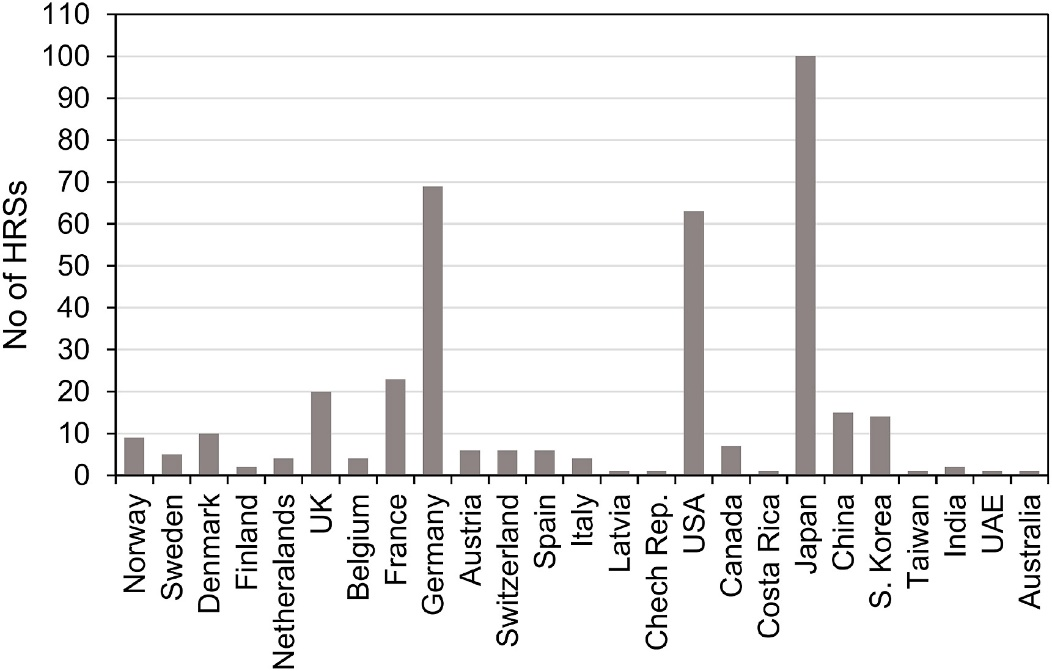
\includegraphics[width=0.6\linewidth]{image/hydrogen_refuel} \caption{Number of hydrogen refuelling stations worldwide (Apostolou and Xydis, 2019)}\label{fig:unnamed-chunk-8}
\end{figure}

The European Strategic Energy Technology Plan proposes hydrogen and fuel-cell technologies as crucial for obtaining green-house gases reduction goals by 2050 (Roadmap Europe H., 2019; Alvarez-Meaza et al., 2020).

\hypertarget{relevant-initiatives-in-austria-35}{%
\subsection*{Relevant initiatives in Austria}\label{relevant-initiatives-in-austria-35}}
\addcontentsline{toc}{subsection}{Relevant initiatives in Austria}

\begin{itemize}
\tightlist
\item
  \href{https://fuelcellsworks.com/news/alstoms-hydrogen-train-successfully-completes-three-months-of-testing-in-austria/\#:~:text=Alstom's\%20Hydrogen\%20Train\%20Successfully\%20Completes\%20Three\%20Months\%20of\%20Testing\%20in\%20Austria,-By\%20FuelCellsWorksDecember\&text=Alstom's\%20Coradia\%20iLint\%2C\%20the\%20world's,Austrian\%20Federal\%20Railways}{hydrogen train}
\end{itemize}

\hypertarget{impacts-with-respect-to-sustainable-development-goals-sdgs-35}{%
\subsection*{Impacts with respect to Sustainable Development Goals (SDGs)}\label{impacts-with-respect-to-sustainable-development-goals-sdgs-35}}
\addcontentsline{toc}{subsection}{Impacts with respect to Sustainable Development Goals (SDGs)}

\begin{longtable}[]{@{}ccccc@{}}
\toprule
\begin{minipage}[b]{0.17\columnwidth}\centering
Impact level\strut
\end{minipage} & \begin{minipage}[b]{0.16\columnwidth}\centering
Indicator\strut
\end{minipage} & \begin{minipage}[b]{0.17\columnwidth}\centering
Impact direction\strut
\end{minipage} & \begin{minipage}[b]{0.17\columnwidth}\centering
Goal description and number\strut
\end{minipage} & \begin{minipage}[b]{0.17\columnwidth}\centering
Source\strut
\end{minipage}\tabularnewline
\midrule
\endhead
\begin{minipage}[t]{0.17\columnwidth}\centering
Individual\strut
\end{minipage} & \begin{minipage}[t]{0.16\columnwidth}\centering
Improved air quality\strut
\end{minipage} & \begin{minipage}[t]{0.17\columnwidth}\centering
\textbf{+}\strut
\end{minipage} & \begin{minipage}[t]{0.17\columnwidth}\centering
Health \& Wellbeing (\emph{3})\strut
\end{minipage} & \begin{minipage}[t]{0.17\columnwidth}\centering
Colella, Jacobson \& Golden, 2005\strut
\end{minipage}\tabularnewline
\begin{minipage}[t]{0.17\columnwidth}\centering
Individual\strut
\end{minipage} & \begin{minipage}[t]{0.16\columnwidth}\centering
High prices of hydrogen cars and hydrogen fuel\strut
\end{minipage} & \begin{minipage}[t]{0.17\columnwidth}\centering
\textbf{-}\strut
\end{minipage} & \begin{minipage}[t]{0.17\columnwidth}\centering
Equality (\emph{5,10})\strut
\end{minipage} & \begin{minipage}[t]{0.17\columnwidth}\centering
Kanna \& Paturu, 2020\strut
\end{minipage}\tabularnewline
\begin{minipage}[t]{0.17\columnwidth}\centering
Individual\strut
\end{minipage} & \begin{minipage}[t]{0.16\columnwidth}\centering
Cost for individuals\strut
\end{minipage} & \begin{minipage}[t]{0.17\columnwidth}\centering
\textbf{\textasciitilde{}}\strut
\end{minipage} & \begin{minipage}[t]{0.17\columnwidth}\centering
Sustainable economic development (\emph{8,11})\strut
\end{minipage} & \begin{minipage}[t]{0.17\columnwidth}\centering
Apostolou \& Xydis, 2019\strut
\end{minipage}\tabularnewline
\begin{minipage}[t]{0.17\columnwidth}\centering
Systemic\strut
\end{minipage} & \begin{minipage}[t]{0.16\columnwidth}\centering
Emissions reduced, improved air quality\strut
\end{minipage} & \begin{minipage}[t]{0.17\columnwidth}\centering
\textbf{+}\strut
\end{minipage} & \begin{minipage}[t]{0.17\columnwidth}\centering
Health \& Wellbeing (\emph{3})\strut
\end{minipage} & \begin{minipage}[t]{0.17\columnwidth}\centering
Colella, Jacobson \& Golden, 2005\strut
\end{minipage}\tabularnewline
\begin{minipage}[t]{0.17\columnwidth}\centering
Systemic\strut
\end{minipage} & \begin{minipage}[t]{0.16\columnwidth}\centering
Distribution and allocation of goods worsens\strut
\end{minipage} & \begin{minipage}[t]{0.17\columnwidth}\centering
\textbf{-}\strut
\end{minipage} & \begin{minipage}[t]{0.17\columnwidth}\centering
Equality (\emph{5,10})\strut
\end{minipage} & \begin{minipage}[t]{0.17\columnwidth}\centering
Kanna \& Paturu, 2020\strut
\end{minipage}\tabularnewline
\begin{minipage}[t]{0.17\columnwidth}\centering
Systemic\strut
\end{minipage} & \begin{minipage}[t]{0.16\columnwidth}\centering
Reduced emissions, replacement of fossil fuels, energy transition\strut
\end{minipage} & \begin{minipage}[t]{0.17\columnwidth}\centering
\textbf{+}\strut
\end{minipage} & \begin{minipage}[t]{0.17\columnwidth}\centering
Environmental sustainability (\emph{7,12-13,15})\strut
\end{minipage} & \begin{minipage}[t]{0.17\columnwidth}\centering
Colella, Jacobson \& Golden, 2005\strut
\end{minipage}\tabularnewline
\begin{minipage}[t]{0.17\columnwidth}\centering
Systemic\strut
\end{minipage} & \begin{minipage}[t]{0.16\columnwidth}\centering
Not yet profitable for manufacturers\strut
\end{minipage} & \begin{minipage}[t]{0.17\columnwidth}\centering
\textbf{+}\strut
\end{minipage} & \begin{minipage}[t]{0.17\columnwidth}\centering
Sustainable economic development (\emph{8,11})\strut
\end{minipage} & \begin{minipage}[t]{0.17\columnwidth}\centering
Roadmap Europe, 2019\strut
\end{minipage}\tabularnewline
\begin{minipage}[t]{0.17\columnwidth}\centering
Systemic\strut
\end{minipage} & \begin{minipage}[t]{0.16\columnwidth}\centering
Number of hydrogen refuelling stations increases\strut
\end{minipage} & \begin{minipage}[t]{0.17\columnwidth}\centering
\textbf{+}\strut
\end{minipage} & \begin{minipage}[t]{0.17\columnwidth}\centering
Innovation \& Infrastructure (\emph{9})\strut
\end{minipage} & \begin{minipage}[t]{0.17\columnwidth}\centering
Apostolou \& Xydis, 2019\strut
\end{minipage}\tabularnewline
\begin{minipage}[t]{0.17\columnwidth}\centering
Systemic\strut
\end{minipage} & \begin{minipage}[t]{0.16\columnwidth}\centering
Sharing technologies internationally\strut
\end{minipage} & \begin{minipage}[t]{0.17\columnwidth}\centering
\textbf{+}\strut
\end{minipage} & \begin{minipage}[t]{0.17\columnwidth}\centering
Partnership \& collaborations (\emph{17})\strut
\end{minipage} & \begin{minipage}[t]{0.17\columnwidth}\centering
International Partnership for Hydrogen and Fuel Cells in the Economy, no date\strut
\end{minipage}\tabularnewline
\bottomrule
\end{longtable}

\hypertarget{technology-and-societal-readiness-level-35}{%
\subsection*{Technology and societal readiness level}\label{technology-and-societal-readiness-level-35}}
\addcontentsline{toc}{subsection}{Technology and societal readiness level}

\begin{longtable}[]{@{}cc@{}}
\toprule
TRL & SRL\tabularnewline
\midrule
\endhead
7-8 & 6-8\tabularnewline
\bottomrule
\end{longtable}

\hypertarget{open-questions-35}{%
\subsection*{Open questions}\label{open-questions-35}}
\addcontentsline{toc}{subsection}{Open questions}

\begin{enumerate}
\def\labelenumi{\arabic{enumi}.}
\tightlist
\item
  Who will drive the progress of hydrogen technology in heavy duty mobility in the future?
\item
  How to store large amounts of energy at low weight and in a restricted space within the vehicle? (Roadmap Europe, 2019)
\end{enumerate}

\hypertarget{further-links-29}{%
\subsection*{Further links}\label{further-links-29}}
\addcontentsline{toc}{subsection}{Further links}

\begin{itemize}
\tightlist
\item
  \href{https://www.europarl.europa.eu/news/nl/press-room/20180911IPR13114/more-electric-cars-on-eu-roads-by-2030}{europarlament}
\item
  \href{https://ec.europa.eu/transport/themes/urban/vehicles/road/hydrogen_en}{ec.europa}
\item
  \href{https://www.fch.europa.eu/news/hydrogen-roadmap-europe-sustainable-pathway-european-energy-transition}{fch.europa}
\end{itemize}

\hypertarget{references-35}{%
\subsection*{References}\label{references-35}}
\addcontentsline{toc}{subsection}{References}

\begin{itemize}
\tightlist
\item
  Alvarez-Meaza, I., Zarrabeitia-Bilbao, E., Rio-Belver, R. M., \& Garechana-Anacabe, G. (2020). Fuel-Cell Electric Vehicles: Plotting a Scientific and Technological Knowledge Map. Sustainability, 12(6), 2334.
\item
  Apostolou, D., \& Xydis, G. (2019). A literature review on hydrogen refuelling stations and infrastructure. Current status and future prospects. Renewable and Sustainable Energy Reviews, 113(May), 109292. \url{https://doi.org/10.1016/j.rser.2019.109292}
\item
  Borgstedt, P., Neyer, B., \& Schewe, G. (2017). Paving the road to electric vehicles--A patent analysis of the automotive supply industry. Journal of cleaner production, 167, 75-87.
\item
  Colella, W. G., Jacobson, M. Z., \& Golden, D. M. (2005). Switching to a U.S. hydrogen fuel cell vehicle fleet: The resultant change in emissions, energy use, and greenhouse gases. Journal of Power Sources, 150, 150--181. \url{https://doi.org/https://doi.org/10.1016/j.jpowsour.2005.05.092}
\item
  Doppelbauer, M. (2020). Grundlagen der Elektromobilität. In Grundlagen der Elektromobilität. \url{https://doi.org/10.1007/978-3-658-29730-5}
\item
  Eichlseder, H., Klell, M., \& Trattner, A. (2018). Wasserstoff in der Fahrzeugtechnik. In Wasserstoff in der Fahrzeugtechnik. \url{https://doi.org/10.1007/978-3-8348-9674-2}
\item
  International Partnership for Hydrogen and Fuel Cells in the Economy. (n.d.). No Title. \url{https://www.iphe.net/}
\item
  Iribarren, D., Martín-Gamboa, M., Manzano, J., \& Dufour, J. (2016). Assessing the social acceptance of hydrogen for transportation in Spain: an unintentional focus on target population for a potential hydrogen economy. International journal of hydrogen energy, 41(10), 5203-5208.
\item
  Kanna, I. V., \& Paturu, P. (2020). A study of hydrogen as an alternative fuel. International Journal of Ambient Energy, 41(12), 1433--1436. \url{https://doi.org/10.1080/01430750.2018.1484803}
\item
  Lehmann, J., \& Luschtinetz, T. (2014). Wasserstoff und Brennstoffzellen.
\item
  Roadmap Europe (2019). A sustainable pathway for the European energy transition. Luxembourg: Publications Office of the European Union.
\item
  Pötscher, F., Winter, R., Lichtblau, G., Schreiber, H., \& Kutschera, U. (2014). Ökobilanz alternativer Antriebe -- Elektrofahrzeuge im Vergleich.
\item
  Schabbach, T., \& Wesselak, V. (2020). Energie - Den Erneuerbaren gehört die Zukunft.
\item
  Tanç, B., Arat, H. T., Baltacıoğlu, E., \& Kadir, A. (2019). Overview of the next quarter century vision of hydrogen fuel cell electric vehicles. In International Journal of Hydrogen Energy, Volume 44, Issue 20, (pp.~10120--10128).
\item
  Töpler, J., \& Lehmann, J. (2017). Wasserstoff und Brennstoffzelle - Technologien und Marktkonzepte. In Springer Vieweg.
\end{itemize}

\hypertarget{bev}{%
\section{Battery electric}\label{bev}}

\hypertarget{synonyms-32}{%
\subsection*{Synonyms}\label{synonyms-32}}
\addcontentsline{toc}{subsection}{Synonyms}

\emph{Battery electric vehicle (BEV)}

\hypertarget{definition-36}{%
\subsection*{Definition}\label{definition-36}}
\addcontentsline{toc}{subsection}{Definition}

Transport contributes up to 30\% of climate-relevant greenhouse gas emissions in Austria, with CO\textsubscript{2} playing the largest role here (Bundesministerium für Umwelt, 2019). While the average engine power of vehicles sold annually is increasing (Kreuzer, 2020), the total emissions from the transport sector are also rising (Bundesministerium für Umwelt, 2019). Without a change in mobility behaviour, only a switch to locally emission-free drive technologies, such as BEVs, can help this situation.
BEVs are emission-free in operation (apart from tyre wear and minimal brake dust) and have a battery storage/accumulator installed that is charged at an external charging station. The power conversion takes place in an electric motor. The benefits and drawbacks of BEVs are presented in the table below.

\begin{longtable}[]{@{}cc@{}}
\toprule
\begin{minipage}[b]{0.47\columnwidth}\centering
Advantages\strut
\end{minipage} & \begin{minipage}[b]{0.47\columnwidth}\centering
Disadvantages\strut
\end{minipage}\tabularnewline
\midrule
\endhead
\begin{minipage}[t]{0.47\columnwidth}\centering
\textbf{Lower noise}: Electric motors operate far more quietly than combustion engines. However, in car traffic, most noise is not generated by the engine, but by the interaction of tyres and road surface or - at high speeds - by aerodynamic noises. In these cases, there is no difference between an electric car and a conventional vehicle. It is only above about 25 kilometres per hour that rolling noises are decisive when driving a car. Below this speed, the engine noise is the determining noise source. Therefore, electric cars are quieter in low-speed areas such as residential areas or when starting at intersections and traffic lights.\strut
\end{minipage} & \begin{minipage}[t]{0.47\columnwidth}\centering
\textbf{Range} currently varies from approx. 120 to \textasciitilde{} 600 km. According to the manufacturer, Tesla Model S can drive up to 610 km and thus has the longest possible range among e-cars, the car costs just under 80,000 euros. The range depends on many factors, such as differences in driving style, weather conditions (it only reaches its full capacity in a temperature range between 20 and 40 degrees Celsius), air conditioning usage. Nevertheless, 94\% of all car journeys by the Austrian population are shorter than 50 km.\strut
\end{minipage}\tabularnewline
\begin{minipage}[t]{0.47\columnwidth}\centering
\textbf{Locally emission-free}: BEVs emit no air pollutants when in use. The reduction of greenhouse gases is strongly dependent on the energy sources with which the electricity was produced beforehand and the resulting emissions. The Austrian electricity mix already has a high proportion of renewable energy. The additional electricity demand caused by electromobility is covered many times over by the expansion plans until 2020 for electricity generation from renewable energy sources. This represents an excellent situation for electromobility in Austria.\strut
\end{minipage} & \begin{minipage}[t]{0.47\columnwidth}\centering
\textbf{Electricity requirement}: With an increasing numbers of electric vehicles on Austrian roads, there may be varying loads on the low-voltage grid, which can lead to voltage fluctuations and interruptions. If, consequently, controlled charging is necessary in the medium to long-term, this should be included in the planning and construction of charging points. However, care must be taken to ensure that the control system corresponds to customer interests.\strut
\end{minipage}\tabularnewline
\begin{minipage}[t]{0.47\columnwidth}\centering
\textbf{Acquisition costs}: the cheapest electric cars are already available from 16,000 euros.\strut
\end{minipage} & \begin{minipage}[t]{0.47\columnwidth}\centering
\textbf{System of fast charging} is cost-intensive as well as challenging in terms of safety and is particularly demanding for the electricity grid due to the high power required (\textgreater{} 20 kW per connection). Such charging stations should primarily be installed where it is compatible with the grid and where they are economical. Therefore, a cost-benefit assessment is advisable before installing fast charging stations.\strut
\end{minipage}\tabularnewline
\begin{minipage}[t]{0.47\columnwidth}\centering
\textbf{Charging costs}: If the electric car is charged on household electricity, the costs are just under 28 cents/kWh, at public charging stations they vary between 30-60 cents. For 100 km in an e-car, electricity costs about 4.50 for charging. The corresponding costs for petrol and diesel in comparison: with a consumption of 6 litres of petrol and 5 litres of diesel respectively, currently 8.40 euros and 6.70 euros (Michael, 2020).\strut
\end{minipage} & \begin{minipage}[t]{0.47\columnwidth}\centering
\textbf{Charging time} depends on battery capacity and charging power. At public fast charging stations, the duration is about half an hour to an hour. At a household socket 8-14 hours.\strut
\end{minipage}\tabularnewline
\begin{minipage}[t]{0.47\columnwidth}\centering
\textbf{Charging stations}: The number of charging stations and charging points is steadily increasing in Austria and currently stands at 5,000 publicly accessible charging points. By comparison, there are just under 2800 petrol stations in Austria (Sitte, 2019).\strut
\end{minipage} & \begin{minipage}[t]{0.47\columnwidth}\centering
-\strut
\end{minipage}\tabularnewline
\bottomrule
\end{longtable}

\hypertarget{key-stakeholders-36}{%
\subsection*{Key stakeholders}\label{key-stakeholders-36}}
\addcontentsline{toc}{subsection}{Key stakeholders}

\begin{itemize}
\tightlist
\item
  \textbf{Affected}: Conventional Cars' Drivers, Car Manufacturers, Insurers
\item
  \textbf{Responsible}: National Governments, City Government, Private Companies, International Lobbyists
\end{itemize}

\hypertarget{current-state-of-art-in-research-36}{%
\subsection*{Current state of art in research}\label{current-state-of-art-in-research-36}}
\addcontentsline{toc}{subsection}{Current state of art in research}

Research on this topic focuses mainly on technology performance, component sizing, charging stations and life cycle assessment (LCA).
LCA is a tool to assess the environmental footprint of a product, process or activity throughout its life cycle (Roy et al., 2009).
The main factors influencing the LCA of BEVs are the production of the vehicle and the provision of electricity for its operation. No direct emissions are produced during operation, but the source of electricity supply influences the amount of indirect emissions. Old batteries can be reused as stationary electricity storage units. Recycling the batteries makes it possible to use them again as a source of raw materials.The following raw materials are necessary in the production of battery electric drives: Lithium for the lithium-ion battery, cobalt also for the battery, although the demand is decreasing, and copper as a conductor material. Rare earths are also needed, in particular neodymium and dysprosium for permanent magnets; these are no longer needed when replaced by another motor technology (Doppelbauer, 2020).

Table below compares the CO\textsubscript{2} emissions (in tonnes) during the production of cars with an internal combustion engine (ICE) and battery-powered, considering size of the car. It is clear that during the production process of BEV generates from 3 to 9 tonnes of CO\textsubscript{2} more than ICE (Doppelbauer, 2020).

\begin{longtable}[]{@{}ccccccc@{}}
\toprule
& & ICE & & & BEV &\tabularnewline
\midrule
\endhead
& Small & Medium & Large & Small (30 kWh) & Medium (60 kWh) & Large (90 kWh)\tabularnewline
Body of the car & 2.5 & 3.8 & 5.0 & 2.5 & 3.8 & 5.0\tabularnewline
Additional components & 0.5 & 0.65 & 0.8 & 0.5 & 0.65 & 0.8\tabularnewline
HV System & - & - & - & 0.3 & 0.55 & 0.7\tabularnewline
Propulsion & 0.4 & 0.6 & 0.8 & 0.2 & 0.25 & 0.3\tabularnewline
Production & 1.5 & 1.5 & 1.5 & 1.5 & 1.5 & 1.5\tabularnewline
Battery & - & - & - & 3 & 6 & 9\tabularnewline
\textbf{Total} & \textbf{4.9} & \textbf{6.6} & \textbf{8.1} & \textbf{8} & \textbf{12.8} & \textbf{17.3}\tabularnewline
\bottomrule
\end{longtable}

This life cycle assessment also takes into account current data on the production of battery systems for electric vehicles. Although the production of batteries requires a significant amount of energy and is therefore associated with high emissions, electric vehicles do not have components such as gearboxes and exhaust gas after-treatment and their production-related emissions.
The decisive factor for the greenhouse gas balance of vehicles is, above all, the energy used to operate the vehicle. While the use of fossil energy in petrol and diesel vehicles results in high greenhouse gas emissions, electric vehicles have no direct greenhouse gas emissions in their balance sheet. Taking into account direct and indirect emissions, the use of an electric car powered by electricity from renewable sources can save 80\% of GHG emissions compared to a fossil fuel-powered car. In addition, the use of renewable electricity also significantly reduces nitrogen oxide emissions. Particulate matter emissions, on the other hand, increase slightly, depending on the source of electricity.
The advantages of electric drives are also evident in the cumulative energy consumption, depending on the quality of the electricity. The lower specific consumption compared to fossil-fueled vehicles should be emphasised. This is due to the high efficiency of the electric motor (Fritz et al., 2018).The negative environmental and social impacts of extracting the rare raw materials needed to produce the battery are already being reduced. The German government supports research into the economic use and recovery of raw materials and the reuse of batteries (Second Life). Batteries that require significantly less cobalt are now also available. Industry is also becoming increasingly involved in initiatives for the sustainable supply of the raw material (responsible mining) (Kurzempa, 2018).
In terms of the efficiency of this technology, the well-to-wheel efficiency in Austria is about 69\%. This is a significant efficeinty gain as compared to a fuel cell car with an average well-to-wheel efficiency of about 27\% and a petrol-powered car at about 20\% (Bundesministerium für Umwelt Naturschutz und nukleare Sicherheit, no date). The losses in the electricity grid in Austria are very low and can be estimated in the range of 5\%, which results in a well-to-tank efficiency of 95\% based on 100\% green electricity.
In the course of the charging process, charging losses of 10\% occur due to resistances in the charging cable and the battery. However, an AC/DC voltage converter (rectifier) is connected upstream of the traction battery, which causes a further 5\% energy loss. In order to get the stored energy onto the road, it now flows through a DC/AC voltage converter (inverter) with 5\% energy loss and can finally be transferred to the wheel by an electric motor with 90\% efficiency. The tank-to-wheel efficiency is therefore 73\%. The overall well-to-wheel efficiency of a BEV is 69\%.

\hypertarget{current-state-of-art-in-practice-35}{%
\subsection*{Current state of art in practice}\label{current-state-of-art-in-practice-35}}
\addcontentsline{toc}{subsection}{Current state of art in practice}

The number of e-cars registered worldwide has reached a new record level. At the same time, however, the growth in new registrations weakened. Around 7.9 million e-cars were registered worldwide in 2019. That is almost 2.3 million more than in 2018 - an increase of 40\%.
The number of new electric cars registered worldwide in 2019 was just over 2.3 million - only 4\% or 90,000 cars more than the previous year. In 2018, the increase compared to 2017 was still around 74\%.
According to the Centre for Solar Energy and Hydrogen Research Baden-Württemberg (ZSW), this development is primarily due to a reduction in e-car subsidies in China and the USA. Nevertheless, the previous year's level of new registrations was almost reached in these countries: 1,204,000 new registrations were registered in China (52,000 less), and 329,500 in the USA (31,800 less).
With around 230,000 registered vehicles, Germany is in seventh place in terms of the total number of e-cars after China, the USA, Norway, Japan, France and the UK (Prack, 2020).
But electric power is not just an alternative for personal modes of transport. Increasingly more vehicles in the commercial and public transport sectors are being electrically powered. The larger and heavier a vehicle is, the more difficult it is to electrify it due to the enormous mass of the larger batteries. However, battery technology is constantly developing, and the ranges are increasing. Even heavy semi-trailer trucks could be electrified in the near future. However, they would need batteries and overhead lines on motorways for fast charging along their routes. This is now being tested in Germany. Three routes in Hesse, Schleswig-Holstein and Baden-Württemberg are currently being equipped with overhead lines (see more in section on \protect\hyperlink{ers}{Electric Road Systems}).In many cities, such as Cologne, Berlin and Hamburg, electric buses are already part of regular service. Their electricity needs are met by fast, occasional charging at bus stops and by charging at night in depots. Many German cities plan to use all-electric buses in the near future (Kurzempa, 2018).

\hypertarget{relevant-initiatives-in-austria-36}{%
\subsection*{Relevant initiatives in Austria}\label{relevant-initiatives-in-austria-36}}
\addcontentsline{toc}{subsection}{Relevant initiatives in Austria}

\begin{itemize}
\tightlist
\item
  \href{https://www.oeamtc.at/thema/elektromobilitaet/alles-ueber-elektroautos-35420295}{oeamtc.at}
\item
  \href{https://www.beoe.at/statistik/}{beoe.at}
\end{itemize}

\hypertarget{impacts-with-respect-to-sustainable-development-goals-sdgs-36}{%
\subsection*{Impacts with respect to Sustainable Development Goals (SDGs)}\label{impacts-with-respect-to-sustainable-development-goals-sdgs-36}}
\addcontentsline{toc}{subsection}{Impacts with respect to Sustainable Development Goals (SDGs)}

\begin{longtable}[]{@{}ccccc@{}}
\toprule
\begin{minipage}[b]{0.17\columnwidth}\centering
Impact level\strut
\end{minipage} & \begin{minipage}[b]{0.16\columnwidth}\centering
Indicator\strut
\end{minipage} & \begin{minipage}[b]{0.17\columnwidth}\centering
Impact direction\strut
\end{minipage} & \begin{minipage}[b]{0.17\columnwidth}\centering
Goal description and number\strut
\end{minipage} & \begin{minipage}[b]{0.17\columnwidth}\centering
Source\strut
\end{minipage}\tabularnewline
\midrule
\endhead
\begin{minipage}[t]{0.17\columnwidth}\centering
Individual\strut
\end{minipage} & \begin{minipage}[t]{0.16\columnwidth}\centering
Lower noise\strut
\end{minipage} & \begin{minipage}[t]{0.17\columnwidth}\centering
\textbf{+}\strut
\end{minipage} & \begin{minipage}[t]{0.17\columnwidth}\centering
Health \& Wellbeing (\emph{3})\strut
\end{minipage} & \begin{minipage}[t]{0.17\columnwidth}\centering
Bundesministerium fuer Umwelt, 2019\strut
\end{minipage}\tabularnewline
\begin{minipage}[t]{0.17\columnwidth}\centering
Individual\strut
\end{minipage} & \begin{minipage}[t]{0.16\columnwidth}\centering
Locally emission-free\strut
\end{minipage} & \begin{minipage}[t]{0.17\columnwidth}\centering
\textbf{+}\strut
\end{minipage} & \begin{minipage}[t]{0.17\columnwidth}\centering
Environmental sustainability (\emph{7,12,13,15})\strut
\end{minipage} & \begin{minipage}[t]{0.17\columnwidth}\centering
Bundesministerium fuer Umwelt, 2019\strut
\end{minipage}\tabularnewline
\begin{minipage}[t]{0.17\columnwidth}\centering
Individual\strut
\end{minipage} & \begin{minipage}[t]{0.16\columnwidth}\centering
Reduced travel cost\strut
\end{minipage} & \begin{minipage}[t]{0.17\columnwidth}\centering
\textbf{+}\strut
\end{minipage} & \begin{minipage}[t]{0.17\columnwidth}\centering
Sustainable economic development (\emph{8,11})\strut
\end{minipage} & \begin{minipage}[t]{0.17\columnwidth}\centering
Michael, 2020\strut
\end{minipage}\tabularnewline
\begin{minipage}[t]{0.17\columnwidth}\centering
Systemic\strut
\end{minipage} & \begin{minipage}[t]{0.16\columnwidth}\centering
Emission free but high emissions in production\strut
\end{minipage} & \begin{minipage}[t]{0.17\columnwidth}\centering
\textbf{\textasciitilde{}}\strut
\end{minipage} & \begin{minipage}[t]{0.17\columnwidth}\centering
Environmental sustainability (\emph{7,12,13,15})\strut
\end{minipage} & \begin{minipage}[t]{0.17\columnwidth}\centering
Fritz et al., 2018\strut
\end{minipage}\tabularnewline
\begin{minipage}[t]{0.17\columnwidth}\centering
Systemic\strut
\end{minipage} & \begin{minipage}[t]{0.16\columnwidth}\centering
Increasing number of charging stations\strut
\end{minipage} & \begin{minipage}[t]{0.17\columnwidth}\centering
\textbf{+}\strut
\end{minipage} & \begin{minipage}[t]{0.17\columnwidth}\centering
Innovation \& Infrastructure (\emph{9})\strut
\end{minipage} & \begin{minipage}[t]{0.17\columnwidth}\centering
Sitte, 2019\strut
\end{minipage}\tabularnewline
\begin{minipage}[t]{0.17\columnwidth}\centering
Systemic\strut
\end{minipage} & \begin{minipage}[t]{0.16\columnwidth}\centering
Electric Vehicles Initiative accelerating the introduction and adoption of electric vehicles worldwide\strut
\end{minipage} & \begin{minipage}[t]{0.17\columnwidth}\centering
\textbf{+}\strut
\end{minipage} & \begin{minipage}[t]{0.17\columnwidth}\centering
Partnership \& collaborations (\emph{17})\strut
\end{minipage} & \begin{minipage}[t]{0.17\columnwidth}\centering
IEA, 2020\strut
\end{minipage}\tabularnewline
\bottomrule
\end{longtable}

\hypertarget{technology-and-societal-readiness-level-36}{%
\subsection*{Technology and societal readiness level}\label{technology-and-societal-readiness-level-36}}
\addcontentsline{toc}{subsection}{Technology and societal readiness level}

\begin{longtable}[]{@{}cc@{}}
\toprule
TRL & SRL\tabularnewline
\midrule
\endhead
8-9 & 7-9\tabularnewline
\bottomrule
\end{longtable}

\hypertarget{open-questions-36}{%
\subsection*{Open questions}\label{open-questions-36}}
\addcontentsline{toc}{subsection}{Open questions}

\begin{enumerate}
\def\labelenumi{\arabic{enumi}.}
\tightlist
\item
  How can supply bottlenecks along the value creation chain be addressed?
\item
  What is the potential shift in dependency from oil-producing to lithium producing countries? What is the expected timeframe?
\item
  What is the role of secondary use of vehicle batteries?
\item
  How can local govenments increase consumer awareness about BEVs?
\end{enumerate}

\hypertarget{further-links-30}{%
\subsection*{Further links}\label{further-links-30}}
\addcontentsline{toc}{subsection}{Further links}

\begin{itemize}
\tightlist
\item
  \href{https://www.bmu.de/fileadmin/Daten_BMU/Pools/Broschueren/elektromobilitaet_broschuere_en_bf.pdf}{bmu.de}
\item
  \href{https://publik.tuwien.ac.at/files/publik_272020.pdf}{publik.tuwien.ac.at}
\item
  \href{https://www.isi.fraunhofer.de/content/dam/isi/dokumente/cct/2020/Fact_check_Batteries_for_electric_cars.pdf}{isi.fraunhofer.de}
\item
  \href{https://www.kleinezeitung.at/auto/elektroauto/5479610/Jaenner-bis-Dezember-2020_Das-sind-die-meistverkauften\#image-01_Volkswagen-e-Golf-2017-1600-01_1534157268197687_v0_h}{kleinezeitung.at}
\item
  \href{https://www.volkswagen.at/elektroauto/id-magazin/mobilitaet/elektromobilitaet-europa}{volkswagen.at}
\item
  \href{https://www.adac.de/rund-ums-fahrzeug/elektromobilitaet/kaufen/elektroautos-uebersicht/}{adac.de}
\item
  \href{https://ec.europa.eu/eurostat/databrowser/view/ROAD_EQR_CARPDA__custom_91702/bookmark/table?lang=de\&bookmarkId=7e47ef9d-b80b-4bd6-a35b-046cb5af4500}{ec.europa.eu}
\end{itemize}

\hypertarget{references-36}{%
\subsection*{References}\label{references-36}}
\addcontentsline{toc}{subsection}{References}

\begin{itemize}
\tightlist
\item
  Bundesministerium für Umwelt, N. und nukleare S. (BMU). (2019). Wie umweltfreundlich sind Elektroautos? 1--20. www.bmu.de
\item
  Bundesministerium für Umwelt Naturschutz und nukleare Sicherheit. (n.d.). Effizienz und Kosten: Lohnt sich der Betrieb eines Elektroautos? \textbar{} BMU. Retrieved 19 February 2021, from \url{https://www.bmu.de/themen/luft-laerm-verkehr/verkehr/elektromobilitaet/effizienz-und-kosten/}
\item
  Doppelbauer, M. (2020). Grundlagen der Elektromobilität. In Grundlagen der Elektromobilität. \url{https://doi.org/10.1007/978-3-658-29730-5}
\item
  Eichlseder, H., Klell, M., \& Trattner, A. (2018). Wasserstoff in der Fahrzeugtechnik. In Wasserstoff in der Fahrzeugtechnik. \url{https://doi.org/10.1007/978-3-8348-9674-2}
\item
  Fritz, D., Heinfellner, H., Lichtblau, G., Pölz, W., \& Stranner, G. (2018). Update: Ökobilanz alternativer Antriebe. 1--16. \url{https://umweltbundesamt.at/fileadmin/site/publikationen/DP152.pdf}
\item
  IEA. (2020, October 26). Electric Vehicles Initiative -- Programmes and partnerships - IEA. \url{https://www.iea.org/areas-of-work/programmes-and-partnerships/electric-vehicles-initiative}
\item
  Kreuzer, C. (2020, September 8). Österreicher fahren auf immer PS-stärkere Autos ab \textbar{} Wiener Städtische. \url{https://www.wienerstaedtische.at/unternehmen/presse/pressemeldungen/detail/oesterreicher-fahren-auf-immer-ps-staerkere-autos-ab.html}
\item
  Kurzempa, A. (2018). Electromobility -- what does it mean? AUTOBUSY -- Technika, Eksploatacja, Systemy Transportowe, 19(6), 894--897. \url{https://doi.org/10.24136/atest.2018.197}
\item
  Lehmann, J., \& Luschtinetz, T. (2014). Wasserstoff und Brennstoffzellen.
\item
  Michael. (2020, January 26). Wasserstoff, E-Auto, E-Fuels: Warum das E-Auto die beste Alternative ist \textbar{} Elektroauto-News.net. \url{https://www.elektroauto-news.net/2020/wasserstoff-e-auto-e-fuels-batterieauto-beste-alternative}
\item
  Pötscher, F., Winter, R., Lichtblau, G., Schreiber, H., \& Kutschera, U. (2014). Ökobilanz alternativer Antriebe -- Elektrofahrzeuge im Vergleich.
\item
  Prack, N. (2020, February 27). Anzahl der Elektroautos: Deutschland \& Ausland \textbar{} ADAC. \url{https://www.adac.de/news/statistik-e-autos/}
\item
  Roy, P., Nei, D., Orikasa, T., Xu, Q., Okadome, H., Nakamura, N., \& Shiina, T. (2009). A review of life cycle assessment (LCA) on some food products. Journal of Food Engineering, 90(1), 1--10. \url{https://doi.org/https://doi.org/10.1016/j.jfoodeng.2008.06.016}
\item
  Schabbach, T., \& Wesselak, V. (2020). Energie - Den Erneuerbaren gehört die Zukunft.
\item
  Sitte, P. (2019, January 21). E-Mobilität: Zahl der Ladestationen für Elektroautos steigt weiter an \textbar{} Bundesverband Elektromobilität Österreich (BEÖ), 21.01.2019. \url{https://www.ots.at/presseaussendung/OTS_20190121_OTS0048/e-mobilitaet-zahl-der-ladestationen-fuer-elektroautos-steigt-weiter-an-bild}
\item
  Töpler, J., \& Lehmann, J. (2017). Wasserstoff und Brennstoffzelle - Technologien und Marktkonzepte. In Springer Vieweg.
\end{itemize}

\hypertarget{plugin_hybrid}{%
\section{Plugin hybrid vehicles}\label{plugin_hybrid}}

\hypertarget{synonyms-33}{%
\subsection*{Synonyms}\label{synonyms-33}}
\addcontentsline{toc}{subsection}{Synonyms}

\emph{Hybrid, HEV, PHEV}

\hypertarget{definition-37}{%
\subsection*{Definition}\label{definition-37}}
\addcontentsline{toc}{subsection}{Definition}

Plug-in hybrid vehicles effectively combine the electric drive with either a conventional combustion engine or other engines that use alternative fuels. This has the advantage that the vehicles can travel long distances, but consumption and emissions are reduced. An energy management system ensures that the optimum amount of energy is drawn from the two energy sources while driving. The ratio of energy consumption is influenced by the driving cycle. The faster the vehicle drives, the more energy is needed (Aswin and Senthilmurugan, 2018).

A hybrid vehicle is superior in terms of the reduced carbon footprint, better mileage than conventional vehicles, financial assistance for purchase, lower annual cost and a regenerative braking system. At the same time, the disadvantages include high purchasing cost, lower fuel efficiency because the extra parts installed take up more space and add weight, and higher maintenance costs due to the dual engine. Additionaly, some concerns have been risen about the risk that the battery may explode in the event of an accident (Aswin and Senthilmurugan, 2018).

However, the safety aspect referred to above can be neglected, as the results in the EuroNCAP crash test show that hybrid vehicles are just as safe as vehicles with conventional drive systems. Toyota's Hybrid Synergy Drive technology (HSD) also serves as an example, where Toyota's hybrid system - based on the airbag trigger signal - immediately switches off all electrical systems in the event of an accident and interrupts the battery contact (ADAC, 2019).

Currently, there are several types of hybrid vehicles available on the market:

\begin{itemize}
\tightlist
\item
  Series hybrid
\end{itemize}

The series hybrid model consists of an internal combustion engine that drives a generator instead of driving the wheels directly. The wheels of the car get their power from the electric motors. The generator powers both the charging battery and the wheels of the car. Series hybrids generate the maximum energy at the time of acceleration and return the energy at the time of regenerative braking. The electric vehicles are designed in such a way that a motor is connected to each wheel. The combination of motor and wheel has the disadvantage of increasing mass and thus affecting handling, but the advantage of improved traction control.

\begin{itemize}
\tightlist
\item
  Parallel hybrid
\end{itemize}

The parallel hybrid vehicle is an integration of an electric motor and an internal combustion engine connected in parallel to the mechanical transmission. The parallel hybrid architecture incorporates both the engine and the electric generator into one unit located between the transmission and the combustion engine. The battery is recharged by regenerative braking. There is a mechanical coupling between the engine and the wheel, recharging the battery cannot occur when the car is moving.

\begin{itemize}
\tightlist
\item
  Combine hybrid
\end{itemize}

The combined hybrid vehicle is a fusion of parallel and series hybrid (series-parallel hybrid). There is a double connection (electrical and mechanical) between the drive axle and the engine. The power transmission to the wheels can be either electric or mechanical. At low speeds it behaves like a series hybrid electric vehicle, but at higher speeds series drive trains are less likely to be preferred and the vehicle motor takes over. This model is significantly more expensive than parallel models as they require a mechanically split drive system, an additional generator and high computing power for dual control (Aswin and Senthilmurugan, 2018).

\hypertarget{key-stakeholders-37}{%
\subsection*{Key stakeholders}\label{key-stakeholders-37}}
\addcontentsline{toc}{subsection}{Key stakeholders}

\begin{itemize}
\tightlist
\item
  \textbf{Affected}: Conventional Cars' Drivers
\item
  \textbf{Responsible}: National Governments, Car Manufacturers, International lobbyists, Private Companies
\end{itemize}

\hypertarget{current-state-of-art-in-research-37}{%
\subsection*{Current state of art in research}\label{current-state-of-art-in-research-37}}
\addcontentsline{toc}{subsection}{Current state of art in research}

Current research efforts focus on the reduction of battery size while maintaining the electric driving performance. Therefore, the study by Song et al.~(2018) suggest 30.4 kWh as an optimal battery capacity. Another, large research developments are performed with respect to reduction of emissions and continuous testing of environmental efficiency in comparison to conventional cars. In an ADAC test of plug-in hybrids, just two cars scored well in the Ecotest, namely Hyundai Ioniq and Volvo V60. The Hyundai was very energy-efficient, while the Volvo consumed more energy and emited more carbon dioxide, but its exhaust gases were cleaner. This allowed it to score well in terms of pollutants. However, the test results leave no doubt that large and heavy cars like the BMW X5 and Mercedes GLE, even as plug-in hybrids, consume a lot of energy and therefore cannot be counted as eco-mobiles (Kroher, 2020). Interestingly, recent test conducted on the newest models of PHEV showed that they pollute the environment two to four times more than the manufacturers claim which undermined the public opinion on the environmental advantages offered by the PHEV (Plötz et al., 2020; Bannon, 2020).

\hypertarget{current-state-of-art-in-practice-36}{%
\subsection*{Current state of art in practice}\label{current-state-of-art-in-practice-36}}
\addcontentsline{toc}{subsection}{Current state of art in practice}

The development of the hybrid electric vehicle is evolving into the next generation of the mode of transport, in line with EU's policy aims of reduction of greenhouse gas emissions. Nevertheless, current market penetration is still relatively low, contributing to 1\% of total car registrations (as of 2019). In Europe, the leaders in the uptake of plug-in hybrid vehicles are Finland and Sweden followed by the United Kingdom (European Environment Agency, 2020).

In Austria the number of plug-in hybrid vehicles quadrupled in 2020 from January to October compared to the same period last year. By the end of October, about 5,500 new vehicles of this type had been registered. Of the approximately 14,700 applications for e-car subsidies so far this year, 90 percent are purely electric, ten percent are plug-in hybrids and range extenders (Ortner, 2020).
The results of a study by the Frauenhofer Institute show that the actual climate balance of plug-in hybrid passenger cars is poor, the real CO\textsubscript{2} emissions are twice as high as the values determined in the test cycle, for company cars the real CO\textsubscript{2} emissions are even three to four times as high. The VCÖ calls for a rapid change in the subsidies for plug-in hybrid cars in Austria (VCÖ, 2020).

By 2020, there are already 800 public e-charging points in Vienna, with number close to a thousand, Vienna is one of the leading e-mobility cities in Europe (Fischer, 2020).The Austrian energy companies - members of the BEÖ - have driven the expansion of the public charging infrastructure in recent years. With over 5,000 charging points between Vienna and Bregenz, Austria provides one of the densest charging networks in Europe (Sitte, 2020b).
Until now, all building owners had to agree to the installation of an e-charging station. This unanimity is to fall soon. Accordingly, the installation of charging stations in apartment buildings will be made easier from autumn onwards (Sitte, 2020a).

\hypertarget{relevant-initiatives-in-austria-37}{%
\subsection*{Relevant initiatives in Austria}\label{relevant-initiatives-in-austria-37}}
\addcontentsline{toc}{subsection}{Relevant initiatives in Austria}

\begin{itemize}
\tightlist
\item
  \href{https://www.oesterreich.gv.at/themen/bauen_wohnen_und_umwelt/elektroautos_und_e_mobilitaet/Seite.4320010.html}{oesterreich.gv}
\item
  \href{https://www.vcoe.at/presse/presseaussendungen/detail/vcoe-neue-studie-zeigt-schlechte-klimabilanz-von-plug-in-hybrid-pkw}{vcoe.at}
\end{itemize}

\hypertarget{impacts-with-respect-to-sustainable-development-goals-sdgs-37}{%
\subsection*{Impacts with respect to Sustainable Development Goals (SDGs)}\label{impacts-with-respect-to-sustainable-development-goals-sdgs-37}}
\addcontentsline{toc}{subsection}{Impacts with respect to Sustainable Development Goals (SDGs)}

\begin{longtable}[]{@{}ccccc@{}}
\toprule
\begin{minipage}[b]{0.17\columnwidth}\centering
Impact level\strut
\end{minipage} & \begin{minipage}[b]{0.16\columnwidth}\centering
Indicator\strut
\end{minipage} & \begin{minipage}[b]{0.17\columnwidth}\centering
Impact direction\strut
\end{minipage} & \begin{minipage}[b]{0.17\columnwidth}\centering
Goal description and number\strut
\end{minipage} & \begin{minipage}[b]{0.17\columnwidth}\centering
Source\strut
\end{minipage}\tabularnewline
\midrule
\endhead
\begin{minipage}[t]{0.17\columnwidth}\centering
Individual\strut
\end{minipage} & \begin{minipage}[t]{0.16\columnwidth}\centering
Carbon dioxide emissions reduced\strut
\end{minipage} & \begin{minipage}[t]{0.17\columnwidth}\centering
\textbf{+}\strut
\end{minipage} & \begin{minipage}[t]{0.17\columnwidth}\centering
Health \& Wellbeing (\emph{3})\strut
\end{minipage} & \begin{minipage}[t]{0.17\columnwidth}\centering
Koellner, 2020\strut
\end{minipage}\tabularnewline
\begin{minipage}[t]{0.17\columnwidth}\centering
Individual\strut
\end{minipage} & \begin{minipage}[t]{0.16\columnwidth}\centering
Number of e-chargining points increases\strut
\end{minipage} & \begin{minipage}[t]{0.17\columnwidth}\centering
\textbf{+}\strut
\end{minipage} & \begin{minipage}[t]{0.17\columnwidth}\centering
Innovation \& Infrastructure (\emph{9})\strut
\end{minipage} & \begin{minipage}[t]{0.17\columnwidth}\centering
Sitte, 2020a\strut
\end{minipage}\tabularnewline
\begin{minipage}[t]{0.17\columnwidth}\centering
Systemic\strut
\end{minipage} & \begin{minipage}[t]{0.16\columnwidth}\centering
Emissions reduced for small and light vehicles only\strut
\end{minipage} & \begin{minipage}[t]{0.17\columnwidth}\centering
\textbf{\textasciitilde{}}\strut
\end{minipage} & \begin{minipage}[t]{0.17\columnwidth}\centering
Environmental sustainability (\emph{7,12-13,15})\strut
\end{minipage} & \begin{minipage}[t]{0.17\columnwidth}\centering
Kroher, 2020; VCOE, 2020\strut
\end{minipage}\tabularnewline
\begin{minipage}[t]{0.17\columnwidth}\centering
Systemic\strut
\end{minipage} & \begin{minipage}[t]{0.16\columnwidth}\centering
Exhaust gas treatment strategies are developed\strut
\end{minipage} & \begin{minipage}[t]{0.17\columnwidth}\centering
\textbf{+}\strut
\end{minipage} & \begin{minipage}[t]{0.17\columnwidth}\centering
Innovation \& Infrastructure (\emph{9})\strut
\end{minipage} & \begin{minipage}[t]{0.17\columnwidth}\centering
Schaefer, 2020\strut
\end{minipage}\tabularnewline
\bottomrule
\end{longtable}

\hypertarget{technology-and-societal-readiness-level-37}{%
\subsection*{Technology and societal readiness level}\label{technology-and-societal-readiness-level-37}}
\addcontentsline{toc}{subsection}{Technology and societal readiness level}

\begin{longtable}[]{@{}cc@{}}
\toprule
TRL & SRL\tabularnewline
\midrule
\endhead
8-9 & 7-9\tabularnewline
\bottomrule
\end{longtable}

\hypertarget{open-questions-37}{%
\subsection*{Open questions}\label{open-questions-37}}
\addcontentsline{toc}{subsection}{Open questions}

\begin{enumerate}
\def\labelenumi{\arabic{enumi}.}
\tightlist
\item
  How the increased use of PHEV will influence the market of second-hand cars?
\item
  What is the impact of batteries on the life cycle of the car?
\end{enumerate}

\hypertarget{further-links-31}{%
\subsection*{Further links}\label{further-links-31}}
\addcontentsline{toc}{subsection}{Further links}

\begin{itemize}
\tightlist
\item
  \href{https://www.europarl.europa.eu/news/nl/press-room/20180911IPR13114/more-electric-cars-on-eu-roads-by-2030}{europarlament}
\item
  \href{https://ec.europa.eu/transport/themes/urban/vehicles/road/hydrogen_en}{ec.europa}
\item
  \href{https://www.fch.europa.eu/news/hydrogen-roadmap-europe-sustainable-pathway-european-energy-transition}{fch.europa}
\end{itemize}

\hypertarget{references-37}{%
\subsection*{References}\label{references-37}}
\addcontentsline{toc}{subsection}{References}

\begin{itemize}
\tightlist
\item
  ADAC. (2019). Hybridantrieb: Funktionsweise sowie Vor- und Nachteile. \url{https://www.adac.de/verkehr/tanken-kraftstoff-antrieb/alternative-antriebe/hybridantrieb/}
\item
  Aswin, A., \& Senthilmurugan, S. (2018). A survey on power levels of battery charging and infrastructure for plug-in electric and hybrid vehicles. IOP Conference Series: Materials Science and Engineering, 402(1). \url{https://doi.org/10.1088/1757-899X/402/1/012154}
\item
  Bannon, E., (2020). Plug-In Hybrids In New Emissions Scandal As Tests Show Higher Pollution Than Claimed \textbar{} Transport \& Environment. {[}online{]} Transportenvironment.org. Available at: \url{https://www.transportenvironment.org/press/plug-hybrids-new-emissions-scandal-tests-show-higher-pollution-claimed} {[}Accessed 19 January 2021{]}.
\item
  European Environment Agency. (2020). INDICATOR ASSESSMENT New Registrations Of Electric Vehicles In Europe. {[}online{]} Available at: \url{https://www.eea.europa.eu/data-and-maps/indicators/proportion-of-vehicle-fleet-meeting-5/assessment} {[}Accessed 19 January 2021{]}
\item
  Fischer, S. M. (2020, September 2). Ökostrom an jeder Ecke: Ladestellen-Ausbau auf Zielgeraden \textbar{} Wien Energie GmbH, 02.09.2020. \url{https://www.ots.at/presseaussendung/OTS_20200902_OTS0138/oekostrom-an-jeder-ecke-ladestellen-ausbau-auf-zielgeraden}
\item
  Köllner, C. (2020). Das sollten Sie über Plug-in-Hybride wissen. \url{https://www.springerprofessional.de/plug-in-hybrid/antriebsstrang/das-sollten-sie-ueber-plug-in-hybride-wissen/18235362}
\item
  Kroher, T. (2020). Plug-in-Hybrid: Modelle, Verbrauch, Technik, Kosten, Ökobilanz. \url{https://www.adac.de/rund-ums-fahrzeug/autokatalog/marken-modelle/auto/plug-in-hybrid/}
\item
  Ortner, M. (2020, December 9). Plug-in-Hybride sind nur so umweltfreundlich wie ihre Fahrer - Wiener Zeitung Online. \url{https://www.wienerzeitung.at/nachrichten/wirtschaft/oesterreich/2084730-Plug-In-Hybride-nur-so-umweltfreundlich-wie-ihre-Fahrer.html}
\item
  Plötz, P., Moll, C., Biecker, G., Mock, P., \& Li, Y. (2020). Real-World Usage of Plug-in Hybrid Electric Vehicles: Fuel Consumption, Electric Driving, and CO₂ Emissions.
\item
  Schäfer, P. (2020). Empa errechnet beste Kaltstart-Strategie für Hybridfahrzeuge. \url{https://www.springerprofessional.de/hybridtechnik/abgasnachbehandlung/empa-errechnet-beste-kaltstart-strategie-fuer-hybridfahrzeuge/17751190}
\item
  Sitte, P. (2020a, June 29). BEÖ begrüßt E-Mobilitätsförderung 2020 \textbar{} Bundesverband Elektromobilität Österreich (BEÖ), 29.06.2020. \url{https://www.ots.at/presseaussendung/OTS_20200629_OTS0144/beoe-begruesst-e-mobilitaetsfoerderung-2020}
\item
  Sitte, P. (2020b, July 15). BEÖ: Strom laden in eigener Garage wird einfacher. Wichtiger Schritt für E-Mobilität. \textbar{} Bundesverband Elektromobilität Österreich (BEÖ), 15.07.2020. \url{https://www.ots.at/presseaussendung/OTS_20200715_OTS0148/beoe-strom-laden-in-eigener-garage-wird-einfacher-wichtiger-schritt-fuer-e-mobilitaet}
\item
  Song, Z., Zhang, X., Li, J., Hofmann, H., Ouyang, M., \& Du, J. (2018). Component sizing optimization of plug-in hybrid electric vehicles with the hybrid energy storage system. Energy, 144, 393--403. \url{https://doi.org/10.1016/j.energy.2017.12.009}
\item
  VCÖ. (2020). VCÖ: Neue Studie zeigt schlechte Klimabilanz von Plug-In-Hybrid Pkw - Mobilität mit Zukunft. \url{https://www.vcoe.at/presse/presseaussendungen/detail/vcoe-neue-studie-zeigt-schlechte-klimabilanz-von-plug-in-hybrid-pkw}
\end{itemize}

\hypertarget{reference}{%
\chapter{References}\label{reference}}

\begin{itemize}
\tightlist
\item
  Lovelace, R., Nowosad, J., Muenchow J. (2021) \emph{Geocomputation with R.} \url{https://geocompr.robinlovelace.net/}
\item
  Afrimap team. \emph{Afrimapr book.} \url{https://github.com/afrimapr/afrimapr-book}
\item
  Xie, Y. (2015). \emph{Dynamic Documents with R and Knitr.} 2nd ed.~Boca Raton, Florida: Chapman; Hall/CRC. \url{http://yihui.org/knitr/}.
\item
  Xie, Y. (2021). \emph{bookdown: Authoring Books and Technical Documents with R Markdown.} \url{https://bookdown.org/yihui/bookdown/}
\end{itemize}

  \bibliography{book.bib,packages.bib}

\end{document}
